\documentclass[a4paper]{book}
\usepackage{a4wide}
\usepackage{makeidx}
\usepackage{fancyhdr}
\usepackage{graphicx}
\usepackage{multicol}
\usepackage{float}
\usepackage{textcomp}
\usepackage{alltt}
\usepackage{times}
\usepackage{ifpdf}
\ifpdf
\usepackage[pdftex,
            pagebackref=true,
            colorlinks=true,
            linkcolor=blue,
            unicode
           ]{hyperref}
\else
\usepackage[ps2pdf,
            pagebackref=true,
            colorlinks=true,
            linkcolor=blue,
            unicode
           ]{hyperref}
\usepackage{pspicture}
\fi
\usepackage[utf8]{inputenc}
\usepackage{doxygen}
\makeindex
\setcounter{tocdepth}{1}
\renewcommand{\footrulewidth}{0.4pt}
\begin{document}
\begin{titlepage}
\vspace*{7cm}
\begin{center}
{\Large Arrow \\[1ex]\large 2.0 }\\
\vspace*{1cm}
{\large Generated by Doxygen 1.5.5}\\
\vspace*{0.5cm}
{\small Thu Jul 3 00:09:10 2008}\\
\end{center}
\end{titlepage}
\clearemptydoublepage
\pagenumbering{roman}
\tableofcontents
\clearemptydoublepage
\pagenumbering{arabic}
\chapter{Data Structure Index}
\section{Data Structures}
Here are the data structures with brief descriptions:\begin{CompactList}
\item\contentsline{section}{\hyperlink{structabtsp__data}{abtsp\_\-data} }{\pageref{structabtsp__data}}{}
\item\contentsline{section}{\hyperlink{structarrow__bintree}{arrow\_\-bintree} (Binary tree data structure )}{\pageref{structarrow__bintree}}{}
\item\contentsline{section}{\hyperlink{structarrow__bintree__node}{arrow\_\-bintree\_\-node} (Binary tree node )}{\pageref{structarrow__bintree__node}}{}
\item\contentsline{section}{\hyperlink{structarrow__bound__result}{arrow\_\-bound\_\-result} (A lower bound result )}{\pageref{structarrow__bound__result}}{}
\item\contentsline{section}{\hyperlink{structarrow__btsp__fun}{arrow\_\-btsp\_\-fun} (BTSP Cost matrix function definition )}{\pageref{structarrow__btsp__fun}}{}
\item\contentsline{section}{\hyperlink{structarrow__btsp__params}{arrow\_\-btsp\_\-params} (BTSP algorithm parameters )}{\pageref{structarrow__btsp__params}}{}
\item\contentsline{section}{\hyperlink{structarrow__btsp__result}{arrow\_\-btsp\_\-result} (BTSP result )}{\pageref{structarrow__btsp__result}}{}
\item\contentsline{section}{\hyperlink{structarrow__btsp__solve__plan}{arrow\_\-btsp\_\-solve\_\-plan} (BTSP feasibility solve step plan )}{\pageref{structarrow__btsp__solve__plan}}{}
\item\contentsline{section}{\hyperlink{structarrow__hash}{arrow\_\-hash} (Hashtable )}{\pageref{structarrow__hash}}{}
\item\contentsline{section}{\hyperlink{structarrow__heap}{arrow\_\-heap} (Binary heap )}{\pageref{structarrow__heap}}{}
\item\contentsline{section}{\hyperlink{structarrow__llist}{arrow\_\-llist} (Linked list data structure )}{\pageref{structarrow__llist}}{}
\item\contentsline{section}{\hyperlink{structarrow__llist__item}{arrow\_\-llist\_\-item} (Linked list item )}{\pageref{structarrow__llist__item}}{}
\item\contentsline{section}{\hyperlink{structarrow__option}{arrow\_\-option} (Program options structure )}{\pageref{structarrow__option}}{}
\item\contentsline{section}{\hyperlink{structarrow__problem}{arrow\_\-problem} (Problem data structure )}{\pageref{structarrow__problem}}{}
\item\contentsline{section}{\hyperlink{structarrow__problem__info}{arrow\_\-problem\_\-info} (Problem information data structure )}{\pageref{structarrow__problem__info}}{}
\item\contentsline{section}{\hyperlink{structarrow__tsp__cc__lk__params}{arrow\_\-tsp\_\-cc\_\-lk\_\-params} (LK algorithm parameters )}{\pageref{structarrow__tsp__cc__lk__params}}{}
\item\contentsline{section}{\hyperlink{structarrow__tsp__rai__params}{arrow\_\-tsp\_\-rai\_\-params} (LK algorithm parameters )}{\pageref{structarrow__tsp__rai__params}}{}
\item\contentsline{section}{\hyperlink{structarrow__tsp__result}{arrow\_\-tsp\_\-result} (TSP result (including result from LK heuristic) )}{\pageref{structarrow__tsp__result}}{}
\item\contentsline{section}{\hyperlink{structcbtsp__basic__data}{cbtsp\_\-basic\_\-data} (Info for basic constrained cost matrix function )}{\pageref{structcbtsp__basic__data}}{}
\item\contentsline{section}{\hyperlink{structcbtsp__shake__data}{cbtsp\_\-shake\_\-data} (Info for shake constrained cost matrix function )}{\pageref{structcbtsp__shake__data}}{}
\item\contentsline{section}{\hyperlink{structfull__matrix__data}{full\_\-matrix\_\-data} }{\pageref{structfull__matrix__data}}{}
\item\contentsline{section}{\hyperlink{structfun__data}{fun\_\-data} }{\pageref{structfun__data}}{}
\end{CompactList}

\chapter{File Index}
\section{File List}
Here is a list of all files with brief descriptions:\begin{CompactList}
\item\contentsline{section}{bin/\hyperlink{bin_22mb_8c}{2mb.c} (2-Max Bound solver )}{\pageref{bin_22mb_8c}}{}
\item\contentsline{section}{bin/\hyperlink{abtsp_8c}{abtsp.c} (Asymmetric Bottleneck TSP heuristic )}{\pageref{abtsp_8c}}{}
\item\contentsline{section}{bin/\hyperlink{bin_2bap_8c}{bap.c} (Bottleneck Assignment Problem solver )}{\pageref{bin_2bap_8c}}{}
\item\contentsline{section}{bin/\hyperlink{bin_2bbssp_8c}{bbssp.c} (Bottleneck Biconnected Spanning Subgraph solver )}{\pageref{bin_2bbssp_8c}}{}
\item\contentsline{section}{bin/\hyperlink{bin_2bscssp_8c}{bscssp.c} (Bottleneck strongly connected spanning subgraph problem solver )}{\pageref{bin_2bscssp_8c}}{}
\item\contentsline{section}{bin/\hyperlink{bin_2btsp_8c}{btsp.c} (Bottleneck TSP heuristic )}{\pageref{bin_2btsp_8c}}{}
\item\contentsline{section}{bin/\hyperlink{cbtsp_8c}{cbtsp.c} (Constrained Bottleneck TSP heuristic )}{\pageref{cbtsp_8c}}{}
\item\contentsline{section}{bin/\hyperlink{bin_2dcbpb_8c}{dcbpb.c} (Degree Constrained Bottleneck Path Bound solver )}{\pageref{bin_2dcbpb_8c}}{}
\item\contentsline{section}{bin/\hyperlink{hash_8c}{hash.c} (Hash testing )}{\pageref{hash_8c}}{}
\item\contentsline{section}{bin/\hyperlink{histogram__data_8c}{histogram\_\-data.c} (Edge length histogram data collector )}{\pageref{histogram__data_8c}}{}
\item\contentsline{section}{bin/\hyperlink{linkern_8c}{linkern.c} (Lin-Kernighan TSP heuristic )}{\pageref{linkern_8c}}{}
\item\contentsline{section}{bin/\hyperlink{subproblem_8c}{subproblem.c} (Sub-problem generator )}{\pageref{subproblem_8c}}{}
\item\contentsline{section}{bin/\hyperlink{tour__info_8c}{tour\_\-info.c} (Tour information )}{\pageref{tour__info_8c}}{}
\item\contentsline{section}{bin/\hyperlink{bin_2tsp_8c}{tsp.c} (Traveling Salesman Problem solver )}{\pageref{bin_2tsp_8c}}{}
\item\contentsline{section}{lib/\hyperlink{lib_22mb_8c}{2mb.c} (2-max bound implemenation )}{\pageref{lib_22mb_8c}}{}
\item\contentsline{section}{lib/\hyperlink{arrow_8h}{arrow.h} (Header file for the Arrow callable library )}{\pageref{arrow_8h}}{}
\item\contentsline{section}{lib/\hyperlink{lib_2bap_8c}{bap.c} (Bottleneck assignment problem (BAP) implemenation )}{\pageref{lib_2bap_8c}}{}
\item\contentsline{section}{lib/\hyperlink{lib_2bbssp_8c}{bbssp.c} (Bottleneck biconnected spanning subgraph problem implemenation )}{\pageref{lib_2bbssp_8c}}{}
\item\contentsline{section}{lib/\hyperlink{bintree_8c}{bintree.c} (Binary tree implementation )}{\pageref{bintree_8c}}{}
\item\contentsline{section}{lib/\hyperlink{lib_2bscssp_8c}{bscssp.c} (Bottleneck strongly connected spanning subgraph problem implemenation )}{\pageref{lib_2bscssp_8c}}{}
\item\contentsline{section}{lib/\hyperlink{lib_2btsp_8c}{btsp.c} (Bottleneck traveling salesman problem (BTSP) methods )}{\pageref{lib_2btsp_8c}}{}
\item\contentsline{section}{lib/\hyperlink{btsp__fun_8c}{btsp\_\-fun.c} (Cost matrix transformation functions )}{\pageref{btsp__fun_8c}}{}
\item\contentsline{section}{lib/\hyperlink{lib_2dcbpb_8c}{dcbpb.c} (Degree constarined bottleneck paths bound )}{\pageref{lib_2dcbpb_8c}}{}
\item\contentsline{section}{lib/\hyperlink{options_8c}{options.c} (Helper for parsing program options )}{\pageref{options_8c}}{}
\item\contentsline{section}{lib/\hyperlink{problem_8c}{problem.c} (Functions for working with problem data )}{\pageref{problem_8c}}{}
\item\contentsline{section}{lib/\hyperlink{lib_2tsp_8c}{tsp.c} (TSP solver and Lin-Kernighan heuristic )}{\pageref{lib_2tsp_8c}}{}
\item\contentsline{section}{lib/\hyperlink{util_8c}{util.c} (Useful utility functions )}{\pageref{util_8c}}{}
\end{CompactList}

\chapter{Data Structure Documentation}
\hypertarget{structarrow__bintree}{
\section{arrow\_\-bintree Struct Reference}
\label{structarrow__bintree}\index{arrow\_\-bintree@{arrow\_\-bintree}}
}
Binary tree data structure.  


{\tt \#include $<$arrow.h$>$}

Collaboration diagram for arrow\_\-bintree:\nopagebreak
\begin{figure}[H]
\begin{center}
\leavevmode
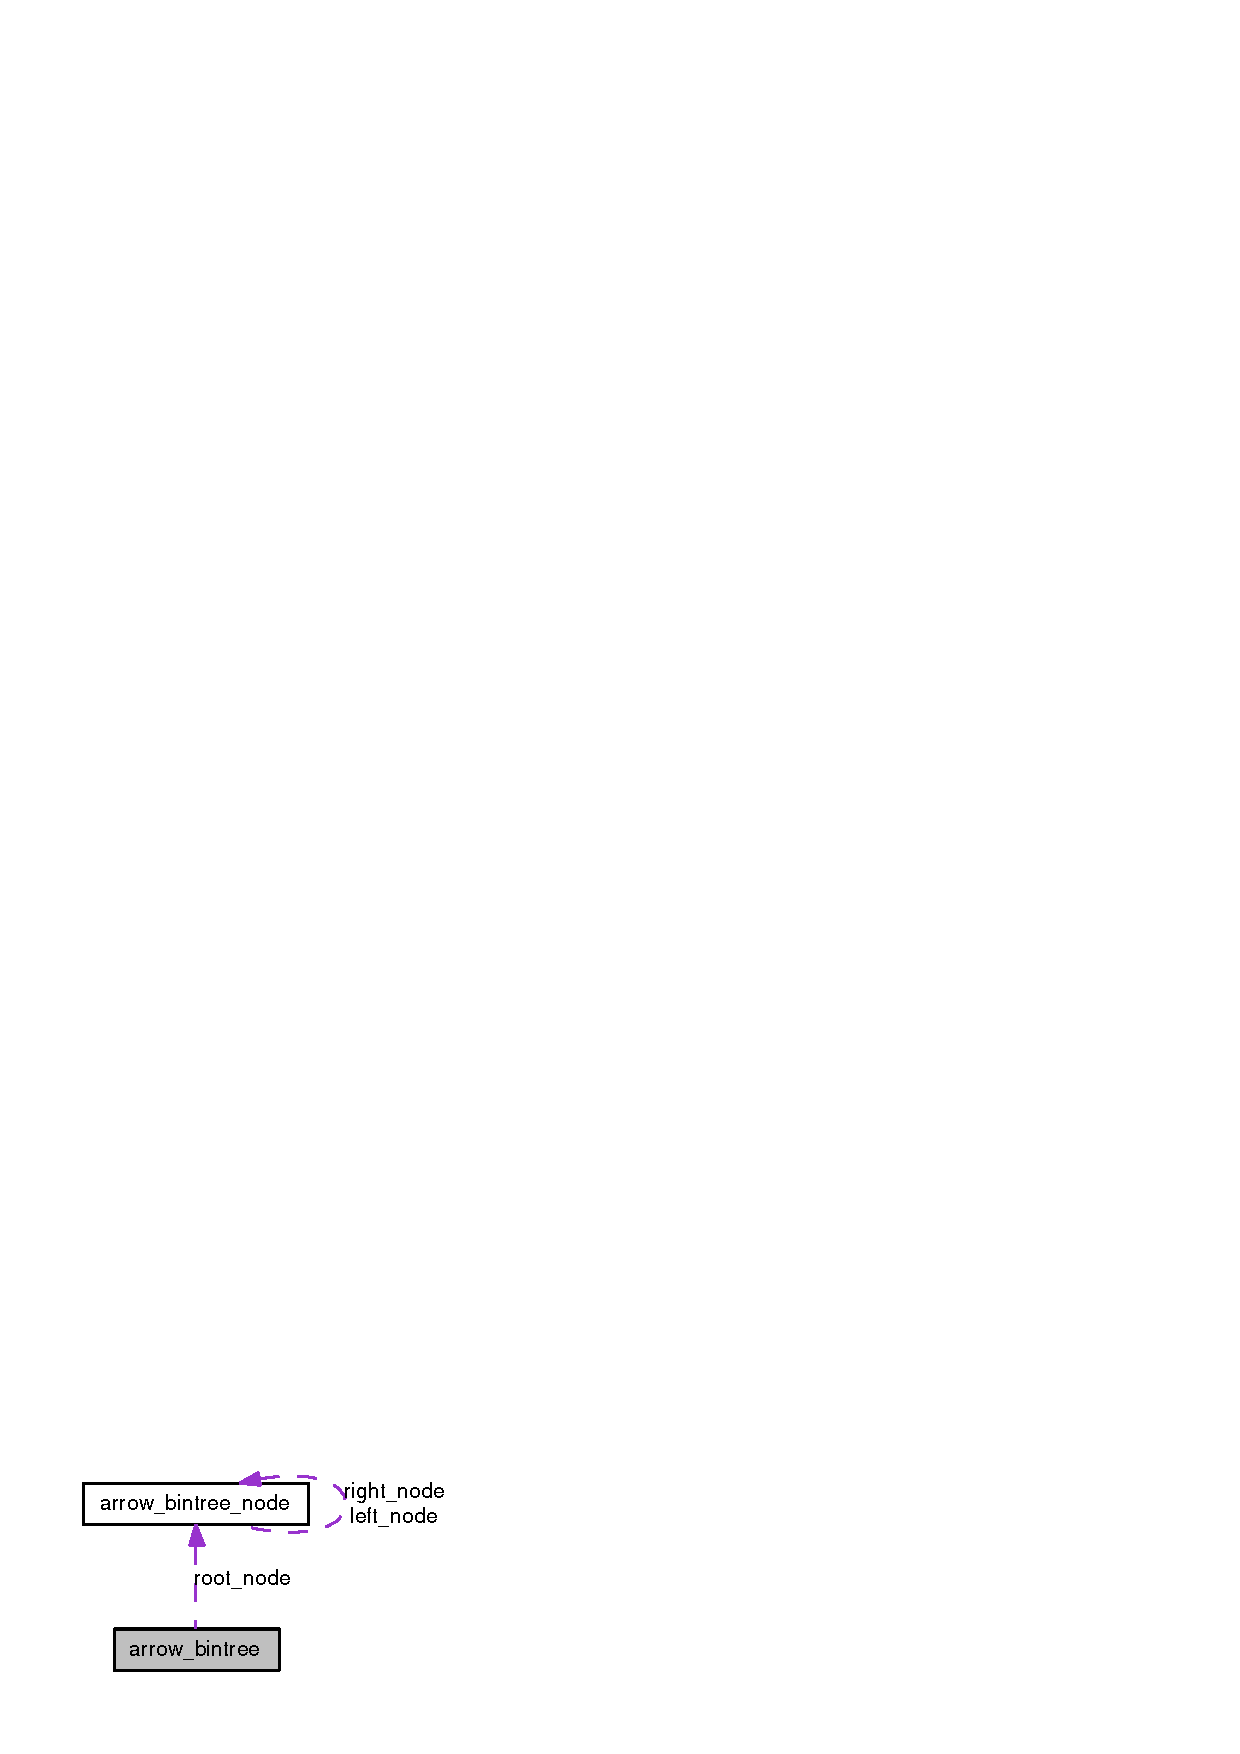
\includegraphics[width=109pt]{structarrow__bintree__coll__graph}
\end{center}
\end{figure}
\subsection*{Data Fields}
\begin{CompactItemize}
\item 
struct \hyperlink{structarrow__bintree__node}{arrow\_\-bintree\_\-node} $\ast$ \hyperlink{structarrow__bintree_09f6d0bd6e32ae2c2f8df57a31388df6}{root\_\-node}
\item 
int \hyperlink{structarrow__bintree_7570628df0b5317cc8e240499ba12974}{size}
\end{CompactItemize}


\subsection{Detailed Description}
Binary tree data structure. 

Definition at line 88 of file arrow.h.

\subsection{Field Documentation}
\hypertarget{structarrow__bintree_09f6d0bd6e32ae2c2f8df57a31388df6}{
\index{arrow\_\-bintree@{arrow\_\-bintree}!root\_\-node@{root\_\-node}}
\index{root\_\-node@{root\_\-node}!arrow_bintree@{arrow\_\-bintree}}
\subsubsection{\setlength{\rightskip}{0pt plus 5cm}struct {\bf arrow\_\-bintree\_\-node}$\ast$ {\bf arrow\_\-bintree::root\_\-node}\hspace{0.3cm}{\tt  \mbox{[}read\mbox{]}}}}
\label{structarrow__bintree_09f6d0bd6e32ae2c2f8df57a31388df6}


root node of tree 

Definition at line 90 of file arrow.h.

Referenced by arrow\_\-bintree\_\-destruct(), arrow\_\-bintree\_\-init(), arrow\_\-bintree\_\-insert(), and arrow\_\-bintree\_\-to\_\-array().\hypertarget{structarrow__bintree_7570628df0b5317cc8e240499ba12974}{
\index{arrow\_\-bintree@{arrow\_\-bintree}!size@{size}}
\index{size@{size}!arrow_bintree@{arrow\_\-bintree}}
\subsubsection{\setlength{\rightskip}{0pt plus 5cm}int {\bf arrow\_\-bintree::size}}}
\label{structarrow__bintree_7570628df0b5317cc8e240499ba12974}


size of tree 

Definition at line 91 of file arrow.h.

Referenced by arrow\_\-bintree\_\-destruct(), arrow\_\-bintree\_\-init(), arrow\_\-bintree\_\-insert(), arrow\_\-bintree\_\-to\_\-array(), arrow\_\-problem\_\-info\_\-get(), constrained\_\-shake\_\-deep\_\-apply(), and insert\_\-at().

The documentation for this struct was generated from the following file:\begin{CompactItemize}
\item 
lib/\hyperlink{arrow_8h}{arrow.h}\end{CompactItemize}

\hypertarget{structarrow__bintree__node}{
\section{arrow\_\-bintree\_\-node Struct Reference}
\label{structarrow__bintree__node}\index{arrow\_\-bintree\_\-node@{arrow\_\-bintree\_\-node}}
}
Binary tree node.  


{\tt \#include $<$arrow.h$>$}

Collaboration diagram for arrow\_\-bintree\_\-node:\nopagebreak
\begin{figure}[H]
\begin{center}
\leavevmode
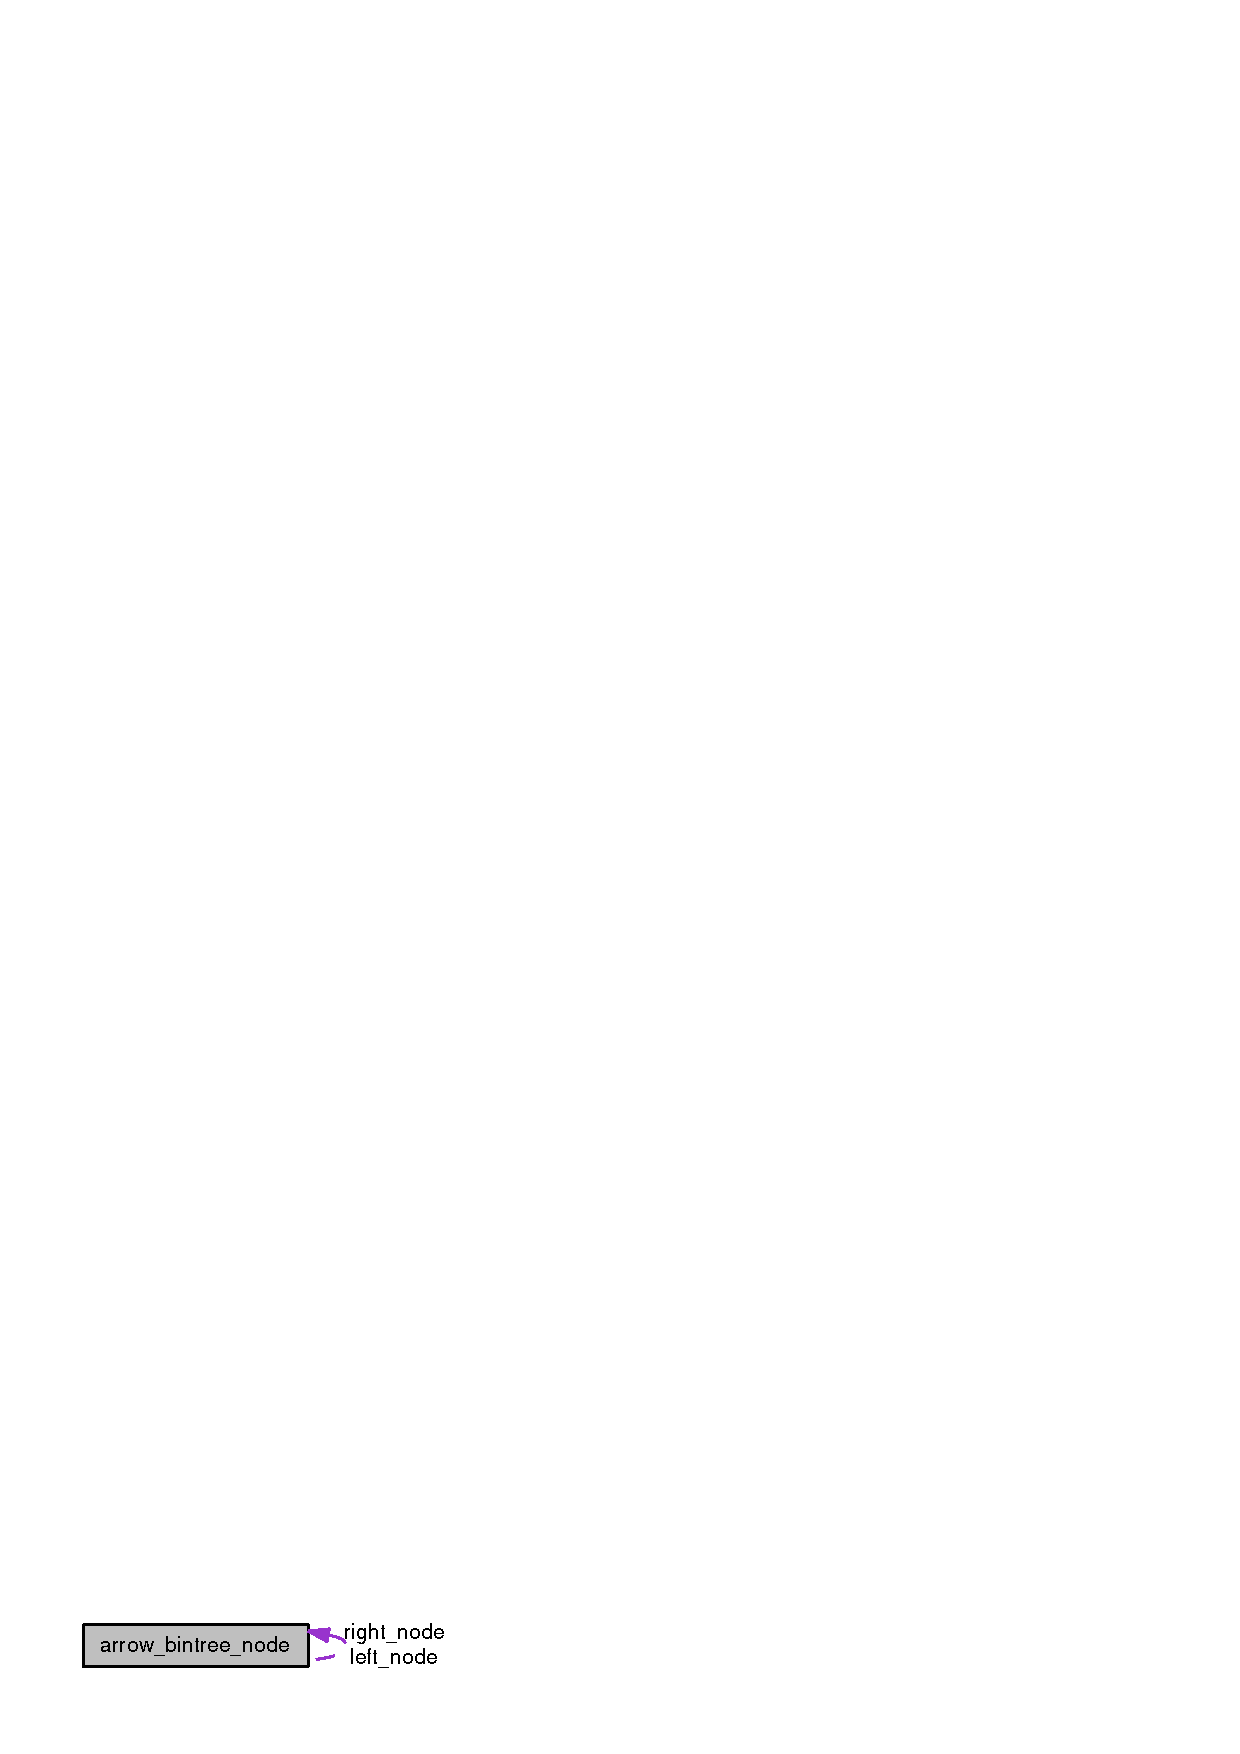
\includegraphics[width=109pt]{structarrow__bintree__node__coll__graph}
\end{center}
\end{figure}
\subsection*{Data Fields}
\begin{CompactItemize}
\item 
int \hyperlink{structarrow__bintree__node_de01c6e7aa823db027836d77e7ce48b6}{data}
\item 
int \hyperlink{structarrow__bintree__node_a359d3d029023fb8763af3329207ee53}{has\_\-left\_\-node}
\item 
int \hyperlink{structarrow__bintree__node_f6f8bb35c520a88841a810777e9bc186}{has\_\-right\_\-node}
\item 
struct \hyperlink{structarrow__bintree__node}{arrow\_\-bintree\_\-node} $\ast$ \hyperlink{structarrow__bintree__node_e7eb125cad02704a57796b16c49b2983}{left\_\-node}
\item 
struct \hyperlink{structarrow__bintree__node}{arrow\_\-bintree\_\-node} $\ast$ \hyperlink{structarrow__bintree__node_4875801983f2b0220212951e6c0130af}{right\_\-node}
\end{CompactItemize}


\subsection{Detailed Description}
Binary tree node. 

Definition at line 97 of file arrow.h.

\subsection{Field Documentation}
\hypertarget{structarrow__bintree__node_de01c6e7aa823db027836d77e7ce48b6}{
\index{arrow\_\-bintree\_\-node@{arrow\_\-bintree\_\-node}!data@{data}}
\index{data@{data}!arrow_bintree_node@{arrow\_\-bintree\_\-node}}
\subsubsection{\setlength{\rightskip}{0pt plus 5cm}int {\bf arrow\_\-bintree\_\-node::data}}}
\label{structarrow__bintree__node_de01c6e7aa823db027836d77e7ce48b6}


data contained in node 

Definition at line 99 of file arrow.h.

Referenced by fill\_\-array(), and insert\_\-at().\hypertarget{structarrow__bintree__node_a359d3d029023fb8763af3329207ee53}{
\index{arrow\_\-bintree\_\-node@{arrow\_\-bintree\_\-node}!has\_\-left\_\-node@{has\_\-left\_\-node}}
\index{has\_\-left\_\-node@{has\_\-left\_\-node}!arrow_bintree_node@{arrow\_\-bintree\_\-node}}
\subsubsection{\setlength{\rightskip}{0pt plus 5cm}int {\bf arrow\_\-bintree\_\-node::has\_\-left\_\-node}}}
\label{structarrow__bintree__node_a359d3d029023fb8763af3329207ee53}


true if left node exists 

Definition at line 100 of file arrow.h.

Referenced by destruct\_\-node(), fill\_\-array(), and insert\_\-at().\hypertarget{structarrow__bintree__node_f6f8bb35c520a88841a810777e9bc186}{
\index{arrow\_\-bintree\_\-node@{arrow\_\-bintree\_\-node}!has\_\-right\_\-node@{has\_\-right\_\-node}}
\index{has\_\-right\_\-node@{has\_\-right\_\-node}!arrow_bintree_node@{arrow\_\-bintree\_\-node}}
\subsubsection{\setlength{\rightskip}{0pt plus 5cm}int {\bf arrow\_\-bintree\_\-node::has\_\-right\_\-node}}}
\label{structarrow__bintree__node_f6f8bb35c520a88841a810777e9bc186}


true if right node exists 

Definition at line 101 of file arrow.h.

Referenced by destruct\_\-node(), fill\_\-array(), and insert\_\-at().\hypertarget{structarrow__bintree__node_e7eb125cad02704a57796b16c49b2983}{
\index{arrow\_\-bintree\_\-node@{arrow\_\-bintree\_\-node}!left\_\-node@{left\_\-node}}
\index{left\_\-node@{left\_\-node}!arrow_bintree_node@{arrow\_\-bintree\_\-node}}
\subsubsection{\setlength{\rightskip}{0pt plus 5cm}struct {\bf arrow\_\-bintree\_\-node}$\ast$ {\bf arrow\_\-bintree\_\-node::left\_\-node}\hspace{0.3cm}{\tt  \mbox{[}read\mbox{]}}}}
\label{structarrow__bintree__node_e7eb125cad02704a57796b16c49b2983}


left node 

Definition at line 102 of file arrow.h.

Referenced by destruct\_\-node(), fill\_\-array(), and insert\_\-at().\hypertarget{structarrow__bintree__node_4875801983f2b0220212951e6c0130af}{
\index{arrow\_\-bintree\_\-node@{arrow\_\-bintree\_\-node}!right\_\-node@{right\_\-node}}
\index{right\_\-node@{right\_\-node}!arrow_bintree_node@{arrow\_\-bintree\_\-node}}
\subsubsection{\setlength{\rightskip}{0pt plus 5cm}struct {\bf arrow\_\-bintree\_\-node}$\ast$ {\bf arrow\_\-bintree\_\-node::right\_\-node}\hspace{0.3cm}{\tt  \mbox{[}read\mbox{]}}}}
\label{structarrow__bintree__node_4875801983f2b0220212951e6c0130af}


right node 

Definition at line 103 of file arrow.h.

Referenced by destruct\_\-node(), fill\_\-array(), and insert\_\-at().

The documentation for this struct was generated from the following file:\begin{CompactItemize}
\item 
lib/\hyperlink{arrow_8h}{arrow.h}\end{CompactItemize}

\hypertarget{structarrow__bound__result}{
\section{arrow\_\-bound\_\-result Struct Reference}
\label{structarrow__bound__result}\index{arrow\_\-bound\_\-result@{arrow\_\-bound\_\-result}}
}
A lower bound result.  


{\tt \#include $<$lb.h$>$}

\subsection*{Data Fields}
\begin{CompactItemize}
\item 
int \hyperlink{structarrow__bound__result_acbca68de984376a60dbb9893935e0f4}{obj\_\-value}
\item 
double \hyperlink{structarrow__bound__result_d27a3cae43bbe1ed2e2c60a4ef307b08}{total\_\-time}
\end{CompactItemize}


\subsection{Detailed Description}
A lower bound result. 

Definition at line 21 of file lb.h.

\subsection{Field Documentation}
\hypertarget{structarrow__bound__result_acbca68de984376a60dbb9893935e0f4}{
\index{arrow\_\-bound\_\-result@{arrow\_\-bound\_\-result}!obj\_\-value@{obj\_\-value}}
\index{obj\_\-value@{obj\_\-value}!arrow_bound_result@{arrow\_\-bound\_\-result}}
\subsubsection{\setlength{\rightskip}{0pt plus 5cm}int {\bf arrow\_\-bound\_\-result::obj\_\-value}}}
\label{structarrow__bound__result_acbca68de984376a60dbb9893935e0f4}


objective value 

Definition at line 23 of file lb.h.

Referenced by arrow\_\-2mb\_\-solve(), arrow\_\-bap\_\-solve(), arrow\_\-bbssp\_\-solve(), arrow\_\-bscssp\_\-solve(), arrow\_\-cbap\_\-solve(), arrow\_\-cbst\_\-solve(), arrow\_\-dcbpb\_\-solve(), and main().\hypertarget{structarrow__bound__result_d27a3cae43bbe1ed2e2c60a4ef307b08}{
\index{arrow\_\-bound\_\-result@{arrow\_\-bound\_\-result}!total\_\-time@{total\_\-time}}
\index{total\_\-time@{total\_\-time}!arrow_bound_result@{arrow\_\-bound\_\-result}}
\subsubsection{\setlength{\rightskip}{0pt plus 5cm}double {\bf arrow\_\-bound\_\-result::total\_\-time}}}
\label{structarrow__bound__result_d27a3cae43bbe1ed2e2c60a4ef307b08}


total time 

Definition at line 24 of file lb.h.

Referenced by arrow\_\-2mb\_\-solve(), arrow\_\-bap\_\-solve(), arrow\_\-bbssp\_\-solve(), arrow\_\-bscssp\_\-solve(), arrow\_\-cbap\_\-solve(), arrow\_\-cbst\_\-solve(), arrow\_\-dcbpb\_\-solve(), and main().

The documentation for this struct was generated from the following file:\begin{CompactItemize}
\item 
include/\hyperlink{lb_8h}{lb.h}\end{CompactItemize}

\hypertarget{structarrow__btsp__fun}{
\section{arrow\_\-btsp\_\-fun Struct Reference}
\label{structarrow__btsp__fun}\index{arrow\_\-btsp\_\-fun@{arrow\_\-btsp\_\-fun}}
}
BTSP Cost matrix function definition.  


{\tt \#include $<$btsp.h$>$}

\subsection*{Data Fields}
\begin{CompactItemize}
\item 
void $\ast$ \hyperlink{structarrow__btsp__fun_9c1a276685fb0cac372faef2dd2ba99a}{data}
\item 
int \hyperlink{structarrow__btsp__fun_1950686e4862a4b1bd68d1ada85e2c79}{shallow}
\item 
int($\ast$ \hyperlink{structarrow__btsp__fun_ffc634f9d1a545f890b0b2007aff544d}{get\_\-cost} )(struct \hyperlink{structarrow__btsp__fun}{arrow\_\-btsp\_\-fun} $\ast$fun, \hyperlink{structarrow__problem}{arrow\_\-problem} $\ast$base\_\-problem, int min\_\-cost, int max\_\-cost, int i, int j)
\begin{CompactList}\small\item\em Retrieves cost between nodes i and j from the function. \item\end{CompactList}\item 
int($\ast$ \hyperlink{structarrow__btsp__fun_c588686921bd526653a7e0d7816aee44}{initialize} )(struct \hyperlink{structarrow__btsp__fun}{arrow\_\-btsp\_\-fun} $\ast$fun)
\begin{CompactList}\small\item\em Initializes the function structure for a new problem. \item\end{CompactList}\item 
void($\ast$ \hyperlink{structarrow__btsp__fun_6c66b7591252728aaa441139c623446a}{destruct} )(struct \hyperlink{structarrow__btsp__fun}{arrow\_\-btsp\_\-fun} $\ast$fun)
\begin{CompactList}\small\item\em Destructs the function structure. \item\end{CompactList}\item 
int($\ast$ \hyperlink{structarrow__btsp__fun_98369e55806c13b3ba90c8c1cbe1f8a4}{feasible} )(struct \hyperlink{structarrow__btsp__fun}{arrow\_\-btsp\_\-fun} $\ast$fun, \hyperlink{structarrow__problem}{arrow\_\-problem} $\ast$base\_\-problem, int min\_\-cost, int max\_\-cost, double tour\_\-length, int $\ast$tour)
\begin{CompactList}\small\item\em Determines if the given tour is feasible or not. \item\end{CompactList}\end{CompactItemize}


\subsection{Detailed Description}
BTSP Cost matrix function definition. 

Definition at line 44 of file btsp.h.

\subsection{Field Documentation}
\hypertarget{structarrow__btsp__fun_9c1a276685fb0cac372faef2dd2ba99a}{
\index{arrow\_\-btsp\_\-fun@{arrow\_\-btsp\_\-fun}!data@{data}}
\index{data@{data}!arrow_btsp_fun@{arrow\_\-btsp\_\-fun}}
\subsubsection[{data}]{\setlength{\rightskip}{0pt plus 5cm}void$\ast$ {\bf arrow\_\-btsp\_\-fun::data}}}
\label{structarrow__btsp__fun_9c1a276685fb0cac372faef2dd2ba99a}


data required by function 

Definition at line 46 of file btsp.h.

Referenced by arrow\_\-baltsp\_\-fun\_\-basic(), arrow\_\-baltsp\_\-fun\_\-dt2(), arrow\_\-baltsp\_\-fun\_\-ib(), arrow\_\-baltsp\_\-fun\_\-shake(), arrow\_\-baltsp\_\-fun\_\-ut(), arrow\_\-btsp\_\-fun\_\-asym\_\-shift(), arrow\_\-btsp\_\-fun\_\-basic(), arrow\_\-btsp\_\-fun\_\-cbtsp\_\-basic(), arrow\_\-btsp\_\-fun\_\-cbtsp\_\-shake(), arrow\_\-btsp\_\-fun\_\-shake\_\-1(), baltsp\_\-dt2\_\-feasible(), baltsp\_\-dt2\_\-get\_\-cost(), baltsp\_\-dt2\_\-initialize(), baltsp\_\-shake\_\-destruct(), baltsp\_\-shake\_\-get\_\-cost(), baltsp\_\-shake\_\-initialize(), btsp\_\-asym\_\-shift\_\-destruct(), btsp\_\-asym\_\-shift\_\-feasible(), btsp\_\-asym\_\-shift\_\-get\_\-cost(), btsp\_\-shake\_\-1\_\-destruct(), btsp\_\-shake\_\-1\_\-get\_\-cost(), btsp\_\-shake\_\-1\_\-initialize(), cbtsp\_\-basic\_\-destruct(), cbtsp\_\-basic\_\-feasible(), cbtsp\_\-basic\_\-get\_\-cost(), cbtsp\_\-shake\_\-destruct(), cbtsp\_\-shake\_\-feasible(), cbtsp\_\-shake\_\-get\_\-cost(), and cbtsp\_\-shake\_\-initialize().\hypertarget{structarrow__btsp__fun_6c66b7591252728aaa441139c623446a}{
\index{arrow\_\-btsp\_\-fun@{arrow\_\-btsp\_\-fun}!destruct@{destruct}}
\index{destruct@{destruct}!arrow_btsp_fun@{arrow\_\-btsp\_\-fun}}
\subsubsection[{destruct}]{\setlength{\rightskip}{0pt plus 5cm}void($\ast$ {\bf arrow\_\-btsp\_\-fun::destruct})(struct {\bf arrow\_\-btsp\_\-fun} $\ast$fun)}}
\label{structarrow__btsp__fun_6c66b7591252728aaa441139c623446a}


Destructs the function structure. 

\begin{Desc}
\item[Parameters:]
\begin{description}
\item[{\em fun}]\mbox{[}out\mbox{]} function structure \end{description}
\end{Desc}


Referenced by arrow\_\-baltsp\_\-fun\_\-basic(), arrow\_\-baltsp\_\-fun\_\-dt2(), arrow\_\-baltsp\_\-fun\_\-ib(), arrow\_\-baltsp\_\-fun\_\-shake(), arrow\_\-baltsp\_\-fun\_\-ut(), arrow\_\-btsp\_\-fun\_\-asym\_\-shift(), arrow\_\-btsp\_\-fun\_\-basic(), arrow\_\-btsp\_\-fun\_\-cbtsp\_\-basic(), arrow\_\-btsp\_\-fun\_\-cbtsp\_\-shake(), arrow\_\-btsp\_\-fun\_\-destruct(), and arrow\_\-btsp\_\-fun\_\-shake\_\-1().\hypertarget{structarrow__btsp__fun_98369e55806c13b3ba90c8c1cbe1f8a4}{
\index{arrow\_\-btsp\_\-fun@{arrow\_\-btsp\_\-fun}!feasible@{feasible}}
\index{feasible@{feasible}!arrow_btsp_fun@{arrow\_\-btsp\_\-fun}}
\subsubsection[{feasible}]{\setlength{\rightskip}{0pt plus 5cm}int($\ast$ {\bf arrow\_\-btsp\_\-fun::feasible})(struct {\bf arrow\_\-btsp\_\-fun} $\ast$fun, {\bf arrow\_\-problem} $\ast$base\_\-problem, int min\_\-cost, int max\_\-cost, double tour\_\-length, int $\ast$tour)}}
\label{structarrow__btsp__fun_98369e55806c13b3ba90c8c1cbe1f8a4}


Determines if the given tour is feasible or not. 

\begin{Desc}
\item[Parameters:]
\begin{description}
\item[{\em fun}]\mbox{[}in\mbox{]} function structure \item[{\em problem}]\mbox{[}in\mbox{]} the problem to check against \item[{\em min\_\-cost}]\mbox{[}in\mbox{]} min\_\-cost to consider for active edges \item[{\em max\_\-cost}]\mbox{[}in\mbox{]} max\_\-cost to consider for active edges \item[{\em tour\_\-length}]\mbox{[}in\mbox{]} the length of the given tour \item[{\em tour}]\mbox{[}in\mbox{]} the tour in node-node format \end{description}
\end{Desc}
\begin{Desc}
\item[Returns:]ARROW\_\-TRUE if the tour is feasible, ARROW\_\-FALSE if not \end{Desc}


Referenced by arrow\_\-baltsp\_\-fun\_\-basic(), arrow\_\-baltsp\_\-fun\_\-dt2(), arrow\_\-baltsp\_\-fun\_\-ib(), arrow\_\-baltsp\_\-fun\_\-shake(), arrow\_\-baltsp\_\-fun\_\-ut(), arrow\_\-btsp\_\-feasible(), arrow\_\-btsp\_\-fun\_\-asym\_\-shift(), arrow\_\-btsp\_\-fun\_\-basic(), arrow\_\-btsp\_\-fun\_\-cbtsp\_\-basic(), arrow\_\-btsp\_\-fun\_\-cbtsp\_\-shake(), and arrow\_\-btsp\_\-fun\_\-shake\_\-1().\hypertarget{structarrow__btsp__fun_ffc634f9d1a545f890b0b2007aff544d}{
\index{arrow\_\-btsp\_\-fun@{arrow\_\-btsp\_\-fun}!get\_\-cost@{get\_\-cost}}
\index{get\_\-cost@{get\_\-cost}!arrow_btsp_fun@{arrow\_\-btsp\_\-fun}}
\subsubsection[{get\_\-cost}]{\setlength{\rightskip}{0pt plus 5cm}int($\ast$ {\bf arrow\_\-btsp\_\-fun::get\_\-cost})(struct {\bf arrow\_\-btsp\_\-fun} $\ast$fun, {\bf arrow\_\-problem} $\ast$base\_\-problem, int min\_\-cost, int max\_\-cost, int i, int j)}}
\label{structarrow__btsp__fun_ffc634f9d1a545f890b0b2007aff544d}


Retrieves cost between nodes i and j from the function. 

\begin{Desc}
\item[Parameters:]
\begin{description}
\item[{\em fun}]\mbox{[}in\mbox{]} function structure \item[{\em problem}]\mbox{[}in\mbox{]} problem structure \item[{\em min\_\-cost}]\mbox{[}in\mbox{]} min\_\-cost to consider for active edges \item[{\em max\_\-cost}]\mbox{[}in\mbox{]} max\_\-cost to consider for active edges \item[{\em i}]\mbox{[}in\mbox{]} id of start node \item[{\em j}]\mbox{[}in\mbox{]} id of end node \end{description}
\end{Desc}
\begin{Desc}
\item[Returns:]cost between node i and node j \end{Desc}


Referenced by apply\_\-deep(), arrow\_\-baltsp\_\-fun\_\-basic(), arrow\_\-baltsp\_\-fun\_\-dt2(), arrow\_\-baltsp\_\-fun\_\-ib(), arrow\_\-baltsp\_\-fun\_\-shake(), arrow\_\-baltsp\_\-fun\_\-ut(), arrow\_\-btsp\_\-fun\_\-asym\_\-shift(), arrow\_\-btsp\_\-fun\_\-basic(), arrow\_\-btsp\_\-fun\_\-cbtsp\_\-basic(), arrow\_\-btsp\_\-fun\_\-cbtsp\_\-shake(), arrow\_\-btsp\_\-fun\_\-shake\_\-1(), and fun\_\-get\_\-cost().\hypertarget{structarrow__btsp__fun_c588686921bd526653a7e0d7816aee44}{
\index{arrow\_\-btsp\_\-fun@{arrow\_\-btsp\_\-fun}!initialize@{initialize}}
\index{initialize@{initialize}!arrow_btsp_fun@{arrow\_\-btsp\_\-fun}}
\subsubsection[{initialize}]{\setlength{\rightskip}{0pt plus 5cm}int($\ast$ {\bf arrow\_\-btsp\_\-fun::initialize})(struct {\bf arrow\_\-btsp\_\-fun} $\ast$fun)}}
\label{structarrow__btsp__fun_c588686921bd526653a7e0d7816aee44}


Initializes the function structure for a new problem. 

\begin{Desc}
\item[Parameters:]
\begin{description}
\item[{\em fun}]\mbox{[}out\mbox{]} function structure \end{description}
\end{Desc}


Referenced by arrow\_\-baltsp\_\-fun\_\-basic(), arrow\_\-baltsp\_\-fun\_\-dt2(), arrow\_\-baltsp\_\-fun\_\-ib(), arrow\_\-baltsp\_\-fun\_\-shake(), arrow\_\-baltsp\_\-fun\_\-ut(), arrow\_\-btsp\_\-fun\_\-apply(), arrow\_\-btsp\_\-fun\_\-asym\_\-shift(), arrow\_\-btsp\_\-fun\_\-basic(), arrow\_\-btsp\_\-fun\_\-cbtsp\_\-basic(), arrow\_\-btsp\_\-fun\_\-cbtsp\_\-shake(), and arrow\_\-btsp\_\-fun\_\-shake\_\-1().\hypertarget{structarrow__btsp__fun_1950686e4862a4b1bd68d1ada85e2c79}{
\index{arrow\_\-btsp\_\-fun@{arrow\_\-btsp\_\-fun}!shallow@{shallow}}
\index{shallow@{shallow}!arrow_btsp_fun@{arrow\_\-btsp\_\-fun}}
\subsubsection[{shallow}]{\setlength{\rightskip}{0pt plus 5cm}int {\bf arrow\_\-btsp\_\-fun::shallow}}}
\label{structarrow__btsp__fun_1950686e4862a4b1bd68d1ada85e2c79}


indicates use of shallow copy of data 

Definition at line 47 of file btsp.h.

Referenced by arrow\_\-baltsp\_\-fun\_\-basic(), arrow\_\-baltsp\_\-fun\_\-dt2(), arrow\_\-baltsp\_\-fun\_\-ib(), arrow\_\-baltsp\_\-fun\_\-shake(), arrow\_\-baltsp\_\-fun\_\-ut(), arrow\_\-btsp\_\-fun\_\-apply(), arrow\_\-btsp\_\-fun\_\-asym\_\-shift(), arrow\_\-btsp\_\-fun\_\-basic(), arrow\_\-btsp\_\-fun\_\-cbtsp\_\-basic(), arrow\_\-btsp\_\-fun\_\-cbtsp\_\-shake(), and arrow\_\-btsp\_\-fun\_\-shake\_\-1().

The documentation for this struct was generated from the following file:\begin{CompactItemize}
\item 
include/\hyperlink{btsp_8h}{btsp.h}\end{CompactItemize}

\hypertarget{structarrow__btsp__params}{
\section{arrow\_\-btsp\_\-params Struct Reference}
\label{structarrow__btsp__params}\index{arrow\_\-btsp\_\-params@{arrow\_\-btsp\_\-params}}
}
BTSP algorithm parameters.  


{\tt \#include $<$arrow.h$>$}

Collaboration diagram for arrow\_\-btsp\_\-params:\nopagebreak
\begin{figure}[H]
\begin{center}
\leavevmode
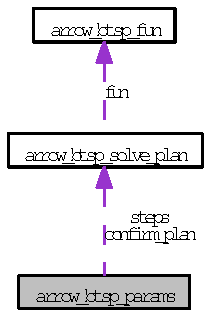
\includegraphics[width=131pt]{structarrow__btsp__params__coll__graph}
\end{center}
\end{figure}
\subsection*{Data Fields}
\begin{CompactItemize}
\item 
int \hyperlink{structarrow__btsp__params_2c579feb3ff41f4d73b5de97596fe465}{confirm\_\-sol}
\item 
int \hyperlink{structarrow__btsp__params_cd85b850ac7c8495a4689100e8c3182c}{supress\_\-ebst}
\item 
int \hyperlink{structarrow__btsp__params_f5fd677200b64930838c6905cbada990}{find\_\-short\_\-tour}
\item 
int \hyperlink{structarrow__btsp__params_da747e3797f9327834e4dbb1459d2786}{lower\_\-bound}
\item 
int \hyperlink{structarrow__btsp__params_b8749004215015a78139b8e4e1fb8905}{upper\_\-bound}
\item 
int \hyperlink{structarrow__btsp__params_2897d24f2fdd53c723609cf68880f55e}{num\_\-steps}
\item 
\hyperlink{structarrow__btsp__solve__plan}{arrow\_\-btsp\_\-solve\_\-plan} $\ast$ \hyperlink{structarrow__btsp__params_49aedb95b2fc4a725e3bb8485470484b}{steps}
\end{CompactItemize}


\subsection{Detailed Description}
BTSP algorithm parameters. 

Definition at line 241 of file arrow.h.

\subsection{Field Documentation}
\hypertarget{structarrow__btsp__params_2c579feb3ff41f4d73b5de97596fe465}{
\index{arrow\_\-btsp\_\-params@{arrow\_\-btsp\_\-params}!confirm\_\-sol@{confirm\_\-sol}}
\index{confirm\_\-sol@{confirm\_\-sol}!arrow_btsp_params@{arrow\_\-btsp\_\-params}}
\subsubsection{\setlength{\rightskip}{0pt plus 5cm}int {\bf arrow\_\-btsp\_\-params::confirm\_\-sol}}}
\label{structarrow__btsp__params_2c579feb3ff41f4d73b5de97596fe465}


confirm sol. with exact solver? 

Definition at line 243 of file arrow.h.

Referenced by arrow\_\-btsp\_\-params\_\-init(), arrow\_\-btsp\_\-solve(), and main().\hypertarget{structarrow__btsp__params_cd85b850ac7c8495a4689100e8c3182c}{
\index{arrow\_\-btsp\_\-params@{arrow\_\-btsp\_\-params}!supress\_\-ebst@{supress\_\-ebst}}
\index{supress\_\-ebst@{supress\_\-ebst}!arrow_btsp_params@{arrow\_\-btsp\_\-params}}
\subsubsection{\setlength{\rightskip}{0pt plus 5cm}int {\bf arrow\_\-btsp\_\-params::supress\_\-ebst}}}
\label{structarrow__btsp__params_cd85b850ac7c8495a4689100e8c3182c}


supress EBST-heuristic? 

Definition at line 244 of file arrow.h.

Referenced by arrow\_\-btsp\_\-params\_\-init(), arrow\_\-btsp\_\-solve(), and main().\hypertarget{structarrow__btsp__params_f5fd677200b64930838c6905cbada990}{
\index{arrow\_\-btsp\_\-params@{arrow\_\-btsp\_\-params}!find\_\-short\_\-tour@{find\_\-short\_\-tour}}
\index{find\_\-short\_\-tour@{find\_\-short\_\-tour}!arrow_btsp_params@{arrow\_\-btsp\_\-params}}
\subsubsection{\setlength{\rightskip}{0pt plus 5cm}int {\bf arrow\_\-btsp\_\-params::find\_\-short\_\-tour}}}
\label{structarrow__btsp__params_f5fd677200b64930838c6905cbada990}


find short BSTP tour? 

Definition at line 245 of file arrow.h.

Referenced by arrow\_\-btsp\_\-params\_\-init(), arrow\_\-btsp\_\-solve(), and main().\hypertarget{structarrow__btsp__params_da747e3797f9327834e4dbb1459d2786}{
\index{arrow\_\-btsp\_\-params@{arrow\_\-btsp\_\-params}!lower\_\-bound@{lower\_\-bound}}
\index{lower\_\-bound@{lower\_\-bound}!arrow_btsp_params@{arrow\_\-btsp\_\-params}}
\subsubsection{\setlength{\rightskip}{0pt plus 5cm}int {\bf arrow\_\-btsp\_\-params::lower\_\-bound}}}
\label{structarrow__btsp__params_da747e3797f9327834e4dbb1459d2786}


initial lower bound 

Definition at line 246 of file arrow.h.

Referenced by arrow\_\-btsp\_\-params\_\-init(), arrow\_\-btsp\_\-solve(), and main().\hypertarget{structarrow__btsp__params_b8749004215015a78139b8e4e1fb8905}{
\index{arrow\_\-btsp\_\-params@{arrow\_\-btsp\_\-params}!upper\_\-bound@{upper\_\-bound}}
\index{upper\_\-bound@{upper\_\-bound}!arrow_btsp_params@{arrow\_\-btsp\_\-params}}
\subsubsection{\setlength{\rightskip}{0pt plus 5cm}int {\bf arrow\_\-btsp\_\-params::upper\_\-bound}}}
\label{structarrow__btsp__params_b8749004215015a78139b8e4e1fb8905}


initial upper bound 

Definition at line 247 of file arrow.h.

Referenced by arrow\_\-btsp\_\-params\_\-init(), arrow\_\-btsp\_\-solve(), and main().\hypertarget{structarrow__btsp__params_2897d24f2fdd53c723609cf68880f55e}{
\index{arrow\_\-btsp\_\-params@{arrow\_\-btsp\_\-params}!num\_\-steps@{num\_\-steps}}
\index{num\_\-steps@{num\_\-steps}!arrow_btsp_params@{arrow\_\-btsp\_\-params}}
\subsubsection{\setlength{\rightskip}{0pt plus 5cm}int {\bf arrow\_\-btsp\_\-params::num\_\-steps}}}
\label{structarrow__btsp__params_2897d24f2fdd53c723609cf68880f55e}


the number of solve plan steps 

Definition at line 248 of file arrow.h.

Referenced by arrow\_\-btsp\_\-params\_\-destruct(), arrow\_\-btsp\_\-params\_\-init(), arrow\_\-btsp\_\-solve(), and main().\hypertarget{structarrow__btsp__params_49aedb95b2fc4a725e3bb8485470484b}{
\index{arrow\_\-btsp\_\-params@{arrow\_\-btsp\_\-params}!steps@{steps}}
\index{steps@{steps}!arrow_btsp_params@{arrow\_\-btsp\_\-params}}
\subsubsection{\setlength{\rightskip}{0pt plus 5cm}{\bf arrow\_\-btsp\_\-solve\_\-plan}$\ast$ {\bf arrow\_\-btsp\_\-params::steps}}}
\label{structarrow__btsp__params_49aedb95b2fc4a725e3bb8485470484b}


solve plan steps 

Definition at line 249 of file arrow.h.

Referenced by arrow\_\-btsp\_\-params\_\-destruct(), arrow\_\-btsp\_\-solve(), and main().

The documentation for this struct was generated from the following file:\begin{CompactItemize}
\item 
lib/\hyperlink{arrow_8h}{arrow.h}\end{CompactItemize}

\hypertarget{structarrow__btsp__result}{
\section{arrow\_\-btsp\_\-result Struct Reference}
\label{structarrow__btsp__result}\index{arrow\_\-btsp\_\-result@{arrow\_\-btsp\_\-result}}
}
BTSP result.  


{\tt \#include $<$btsp.h$>$}

\subsection*{Data Fields}
\begin{CompactItemize}
\item 
int \hyperlink{structarrow__btsp__result_6ba21b4231cfe2c1e437a9f7e8f31aa6}{found\_\-tour}
\item 
int \hyperlink{structarrow__btsp__result_8c80e92a356cdd42d176a3947fcc5665}{min\_\-cost}
\item 
int \hyperlink{structarrow__btsp__result_06f661dc0e63cb5fd1888303b3ec626f}{max\_\-cost}
\item 
double \hyperlink{structarrow__btsp__result_3c0b8827a873df71166e7fe9419c45c2}{tour\_\-length}
\item 
int $\ast$ \hyperlink{structarrow__btsp__result_ebd9a553dc3bf31f52eda0b293b0e272}{tour}
\item 
int \hyperlink{structarrow__btsp__result_febcf61e24bf277eeb7795c18bd42b8b}{optimal}
\item 
int \hyperlink{structarrow__btsp__result_80106c5f0b8f82353ad6771ad9eaac71}{bin\_\-search\_\-steps}
\item 
int \hyperlink{structarrow__btsp__result_b1d423ab6eda81de4c3bde1685976593}{solver\_\-attempts} \mbox{[}ARROW\_\-TSP\_\-SOLVER\_\-COUNT\mbox{]}
\item 
double \hyperlink{structarrow__btsp__result_f13227603570821a0ba7d6466f39f00c}{solver\_\-time} \mbox{[}ARROW\_\-TSP\_\-SOLVER\_\-COUNT\mbox{]}
\item 
double \hyperlink{structarrow__btsp__result_dea5711f0a574d98f66d1b20011a68de}{total\_\-time}
\end{CompactItemize}


\subsection{Detailed Description}
BTSP result. 

Definition at line 27 of file btsp.h.

\subsection{Field Documentation}
\hypertarget{structarrow__btsp__result_80106c5f0b8f82353ad6771ad9eaac71}{
\index{arrow\_\-btsp\_\-result@{arrow\_\-btsp\_\-result}!bin\_\-search\_\-steps@{bin\_\-search\_\-steps}}
\index{bin\_\-search\_\-steps@{bin\_\-search\_\-steps}!arrow_btsp_result@{arrow\_\-btsp\_\-result}}
\subsubsection[{bin\_\-search\_\-steps}]{\setlength{\rightskip}{0pt plus 5cm}int {\bf arrow\_\-btsp\_\-result::bin\_\-search\_\-steps}}}
\label{structarrow__btsp__result_80106c5f0b8f82353ad6771ad9eaac71}


number of steps in binary search 

Definition at line 35 of file btsp.h.

Referenced by arrow\_\-balanced\_\-tsp\_\-db(), arrow\_\-balanced\_\-tsp\_\-dt(), arrow\_\-balanced\_\-tsp\_\-dt2(), arrow\_\-balanced\_\-tsp\_\-ib(), arrow\_\-balanced\_\-tsp\_\-ib2(), arrow\_\-btsp\_\-result\_\-init(), arrow\_\-btsp\_\-result\_\-print\_\-pretty(), arrow\_\-btsp\_\-result\_\-print\_\-xml(), arrow\_\-btsp\_\-solve(), and main().\hypertarget{structarrow__btsp__result_6ba21b4231cfe2c1e437a9f7e8f31aa6}{
\index{arrow\_\-btsp\_\-result@{arrow\_\-btsp\_\-result}!found\_\-tour@{found\_\-tour}}
\index{found\_\-tour@{found\_\-tour}!arrow_btsp_result@{arrow\_\-btsp\_\-result}}
\subsubsection[{found\_\-tour}]{\setlength{\rightskip}{0pt plus 5cm}int {\bf arrow\_\-btsp\_\-result::found\_\-tour}}}
\label{structarrow__btsp__result_6ba21b4231cfe2c1e437a9f7e8f31aa6}


true if a tour was found, false otherwise 

Definition at line 29 of file btsp.h.

Referenced by arrow\_\-balanced\_\-tsp\_\-db(), arrow\_\-balanced\_\-tsp\_\-dt(), arrow\_\-balanced\_\-tsp\_\-dt2(), arrow\_\-balanced\_\-tsp\_\-ib(), arrow\_\-balanced\_\-tsp\_\-ib2(), arrow\_\-btsp\_\-feasible(), arrow\_\-btsp\_\-result\_\-init(), arrow\_\-btsp\_\-result\_\-print\_\-pretty(), arrow\_\-btsp\_\-result\_\-print\_\-xml(), arrow\_\-btsp\_\-solve(), and main().\hypertarget{structarrow__btsp__result_06f661dc0e63cb5fd1888303b3ec626f}{
\index{arrow\_\-btsp\_\-result@{arrow\_\-btsp\_\-result}!max\_\-cost@{max\_\-cost}}
\index{max\_\-cost@{max\_\-cost}!arrow_btsp_result@{arrow\_\-btsp\_\-result}}
\subsubsection[{max\_\-cost}]{\setlength{\rightskip}{0pt plus 5cm}int {\bf arrow\_\-btsp\_\-result::max\_\-cost}}}
\label{structarrow__btsp__result_06f661dc0e63cb5fd1888303b3ec626f}


smallest cost in tour 

Definition at line 31 of file btsp.h.

Referenced by arrow\_\-balanced\_\-tsp\_\-db(), arrow\_\-balanced\_\-tsp\_\-dt(), arrow\_\-balanced\_\-tsp\_\-dt2(), arrow\_\-balanced\_\-tsp\_\-ib(), arrow\_\-balanced\_\-tsp\_\-ib2(), arrow\_\-btsp\_\-feasible(), arrow\_\-btsp\_\-result\_\-init(), arrow\_\-btsp\_\-result\_\-print\_\-pretty(), arrow\_\-btsp\_\-result\_\-print\_\-xml(), arrow\_\-btsp\_\-solve(), and main().\hypertarget{structarrow__btsp__result_8c80e92a356cdd42d176a3947fcc5665}{
\index{arrow\_\-btsp\_\-result@{arrow\_\-btsp\_\-result}!min\_\-cost@{min\_\-cost}}
\index{min\_\-cost@{min\_\-cost}!arrow_btsp_result@{arrow\_\-btsp\_\-result}}
\subsubsection[{min\_\-cost}]{\setlength{\rightskip}{0pt plus 5cm}int {\bf arrow\_\-btsp\_\-result::min\_\-cost}}}
\label{structarrow__btsp__result_8c80e92a356cdd42d176a3947fcc5665}


smallest cost in tour 

Definition at line 30 of file btsp.h.

Referenced by arrow\_\-balanced\_\-tsp\_\-db(), arrow\_\-balanced\_\-tsp\_\-dt(), arrow\_\-balanced\_\-tsp\_\-dt2(), arrow\_\-balanced\_\-tsp\_\-ib(), arrow\_\-balanced\_\-tsp\_\-ib2(), arrow\_\-btsp\_\-feasible(), arrow\_\-btsp\_\-result\_\-init(), arrow\_\-btsp\_\-result\_\-print\_\-pretty(), arrow\_\-btsp\_\-result\_\-print\_\-xml(), arrow\_\-btsp\_\-solve(), and main().\hypertarget{structarrow__btsp__result_febcf61e24bf277eeb7795c18bd42b8b}{
\index{arrow\_\-btsp\_\-result@{arrow\_\-btsp\_\-result}!optimal@{optimal}}
\index{optimal@{optimal}!arrow_btsp_result@{arrow\_\-btsp\_\-result}}
\subsubsection[{optimal}]{\setlength{\rightskip}{0pt plus 5cm}int {\bf arrow\_\-btsp\_\-result::optimal}}}
\label{structarrow__btsp__result_febcf61e24bf277eeb7795c18bd42b8b}


indicates if the solution is optimal 

Definition at line 34 of file btsp.h.

Referenced by arrow\_\-balanced\_\-tsp\_\-db(), arrow\_\-balanced\_\-tsp\_\-dt(), arrow\_\-balanced\_\-tsp\_\-dt2(), arrow\_\-balanced\_\-tsp\_\-ib(), arrow\_\-balanced\_\-tsp\_\-ib2(), arrow\_\-btsp\_\-result\_\-print\_\-pretty(), arrow\_\-btsp\_\-result\_\-print\_\-xml(), and arrow\_\-btsp\_\-solve().\hypertarget{structarrow__btsp__result_b1d423ab6eda81de4c3bde1685976593}{
\index{arrow\_\-btsp\_\-result@{arrow\_\-btsp\_\-result}!solver\_\-attempts@{solver\_\-attempts}}
\index{solver\_\-attempts@{solver\_\-attempts}!arrow_btsp_result@{arrow\_\-btsp\_\-result}}
\subsubsection[{solver\_\-attempts}]{\setlength{\rightskip}{0pt plus 5cm}int {\bf arrow\_\-btsp\_\-result::solver\_\-attempts}\mbox{[}ARROW\_\-TSP\_\-SOLVER\_\-COUNT\mbox{]}}}
\label{structarrow__btsp__result_b1d423ab6eda81de4c3bde1685976593}


calls to solver 

Definition at line 36 of file btsp.h.

Referenced by arrow\_\-balanced\_\-tsp\_\-db(), arrow\_\-balanced\_\-tsp\_\-dt(), arrow\_\-balanced\_\-tsp\_\-dt2(), arrow\_\-balanced\_\-tsp\_\-ib(), arrow\_\-balanced\_\-tsp\_\-ib2(), arrow\_\-btsp\_\-feasible(), arrow\_\-btsp\_\-result\_\-init(), arrow\_\-btsp\_\-result\_\-print\_\-pretty(), arrow\_\-btsp\_\-result\_\-print\_\-xml(), arrow\_\-btsp\_\-solve(), and main().\hypertarget{structarrow__btsp__result_f13227603570821a0ba7d6466f39f00c}{
\index{arrow\_\-btsp\_\-result@{arrow\_\-btsp\_\-result}!solver\_\-time@{solver\_\-time}}
\index{solver\_\-time@{solver\_\-time}!arrow_btsp_result@{arrow\_\-btsp\_\-result}}
\subsubsection[{solver\_\-time}]{\setlength{\rightskip}{0pt plus 5cm}double {\bf arrow\_\-btsp\_\-result::solver\_\-time}\mbox{[}ARROW\_\-TSP\_\-SOLVER\_\-COUNT\mbox{]}}}
\label{structarrow__btsp__result_f13227603570821a0ba7d6466f39f00c}


total time for solver 

Definition at line 37 of file btsp.h.

Referenced by arrow\_\-balanced\_\-tsp\_\-db(), arrow\_\-balanced\_\-tsp\_\-dt(), arrow\_\-balanced\_\-tsp\_\-dt2(), arrow\_\-balanced\_\-tsp\_\-ib(), arrow\_\-balanced\_\-tsp\_\-ib2(), arrow\_\-btsp\_\-feasible(), arrow\_\-btsp\_\-result\_\-init(), arrow\_\-btsp\_\-result\_\-print\_\-pretty(), arrow\_\-btsp\_\-result\_\-print\_\-xml(), arrow\_\-btsp\_\-solve(), and main().\hypertarget{structarrow__btsp__result_dea5711f0a574d98f66d1b20011a68de}{
\index{arrow\_\-btsp\_\-result@{arrow\_\-btsp\_\-result}!total\_\-time@{total\_\-time}}
\index{total\_\-time@{total\_\-time}!arrow_btsp_result@{arrow\_\-btsp\_\-result}}
\subsubsection[{total\_\-time}]{\setlength{\rightskip}{0pt plus 5cm}double {\bf arrow\_\-btsp\_\-result::total\_\-time}}}
\label{structarrow__btsp__result_dea5711f0a574d98f66d1b20011a68de}


total time 

Definition at line 38 of file btsp.h.

Referenced by arrow\_\-balanced\_\-tsp\_\-db(), arrow\_\-balanced\_\-tsp\_\-dt(), arrow\_\-balanced\_\-tsp\_\-dt2(), arrow\_\-balanced\_\-tsp\_\-ib(), arrow\_\-balanced\_\-tsp\_\-ib2(), arrow\_\-btsp\_\-feasible(), arrow\_\-btsp\_\-result\_\-init(), arrow\_\-btsp\_\-result\_\-print\_\-pretty(), arrow\_\-btsp\_\-result\_\-print\_\-xml(), arrow\_\-btsp\_\-solve(), and main().\hypertarget{structarrow__btsp__result_ebd9a553dc3bf31f52eda0b293b0e272}{
\index{arrow\_\-btsp\_\-result@{arrow\_\-btsp\_\-result}!tour@{tour}}
\index{tour@{tour}!arrow_btsp_result@{arrow\_\-btsp\_\-result}}
\subsubsection[{tour}]{\setlength{\rightskip}{0pt plus 5cm}int$\ast$ {\bf arrow\_\-btsp\_\-result::tour}}}
\label{structarrow__btsp__result_ebd9a553dc3bf31f52eda0b293b0e272}


tour that was found in node-node format 

Definition at line 33 of file btsp.h.

Referenced by arrow\_\-balanced\_\-tsp\_\-db(), arrow\_\-balanced\_\-tsp\_\-dt(), arrow\_\-balanced\_\-tsp\_\-dt2(), arrow\_\-balanced\_\-tsp\_\-ib(), arrow\_\-balanced\_\-tsp\_\-ib2(), arrow\_\-btsp\_\-feasible(), arrow\_\-btsp\_\-result\_\-destruct(), arrow\_\-btsp\_\-result\_\-init(), arrow\_\-btsp\_\-solve(), and main().\hypertarget{structarrow__btsp__result_3c0b8827a873df71166e7fe9419c45c2}{
\index{arrow\_\-btsp\_\-result@{arrow\_\-btsp\_\-result}!tour\_\-length@{tour\_\-length}}
\index{tour\_\-length@{tour\_\-length}!arrow_btsp_result@{arrow\_\-btsp\_\-result}}
\subsubsection[{tour\_\-length}]{\setlength{\rightskip}{0pt plus 5cm}double {\bf arrow\_\-btsp\_\-result::tour\_\-length}}}
\label{structarrow__btsp__result_3c0b8827a873df71166e7fe9419c45c2}


length of the tour found 

Definition at line 32 of file btsp.h.

Referenced by arrow\_\-balanced\_\-tsp\_\-db(), arrow\_\-balanced\_\-tsp\_\-dt(), arrow\_\-balanced\_\-tsp\_\-dt2(), arrow\_\-balanced\_\-tsp\_\-ib(), arrow\_\-balanced\_\-tsp\_\-ib2(), arrow\_\-btsp\_\-feasible(), arrow\_\-btsp\_\-result\_\-init(), arrow\_\-btsp\_\-result\_\-print\_\-pretty(), arrow\_\-btsp\_\-result\_\-print\_\-xml(), arrow\_\-btsp\_\-solve(), and main().

The documentation for this struct was generated from the following file:\begin{CompactItemize}
\item 
include/\hyperlink{btsp_8h}{btsp.h}\end{CompactItemize}

\hypertarget{structarrow__btsp__solve__plan}{
\section{arrow\_\-btsp\_\-solve\_\-plan Struct Reference}
\label{structarrow__btsp__solve__plan}\index{arrow\_\-btsp\_\-solve\_\-plan@{arrow\_\-btsp\_\-solve\_\-plan}}
}
BTSP feasibility solve step plan.  


{\tt \#include $<$btsp.h$>$}

Collaboration diagram for arrow\_\-btsp\_\-solve\_\-plan:\nopagebreak
\begin{figure}[H]
\begin{center}
\leavevmode
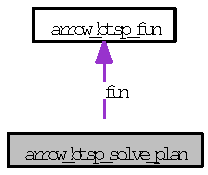
\includegraphics[width=136pt]{structarrow__btsp__solve__plan__coll__graph}
\end{center}
\end{figure}
\subsection*{Data Fields}
\begin{CompactItemize}
\item 
int \hyperlink{structarrow__btsp__solve__plan_911facf12673ddb5c3eb024fa12ee18d}{tsp\_\-solver}
\item 
void $\ast$ \hyperlink{structarrow__btsp__solve__plan_2b7cf65583f45c990218139dbae34ae5}{tsp\_\-params}
\item 
\hyperlink{structarrow__btsp__fun}{arrow\_\-btsp\_\-fun} \hyperlink{structarrow__btsp__solve__plan_89fa2ad1bcc026cd50fd7abc6c30ce3e}{fun}
\item 
int \hyperlink{structarrow__btsp__solve__plan_acfa3d4257a33548a9f60ee568219bc5}{attempts}
\end{CompactItemize}


\subsection{Detailed Description}
BTSP feasibility solve step plan. 

Definition at line 95 of file btsp.h.

\subsection{Field Documentation}
\hypertarget{structarrow__btsp__solve__plan_acfa3d4257a33548a9f60ee568219bc5}{
\index{arrow\_\-btsp\_\-solve\_\-plan@{arrow\_\-btsp\_\-solve\_\-plan}!attempts@{attempts}}
\index{attempts@{attempts}!arrow_btsp_solve_plan@{arrow\_\-btsp\_\-solve\_\-plan}}
\subsubsection[{attempts}]{\setlength{\rightskip}{0pt plus 5cm}int {\bf arrow\_\-btsp\_\-solve\_\-plan::attempts}}}
\label{structarrow__btsp__solve__plan_acfa3d4257a33548a9f60ee568219bc5}


number of attempts to perform 

Definition at line 100 of file btsp.h.

Referenced by arrow\_\-btsp\_\-feasible(), and arrow\_\-btsp\_\-solve\_\-plan\_\-init().\hypertarget{structarrow__btsp__solve__plan_89fa2ad1bcc026cd50fd7abc6c30ce3e}{
\index{arrow\_\-btsp\_\-solve\_\-plan@{arrow\_\-btsp\_\-solve\_\-plan}!fun@{fun}}
\index{fun@{fun}!arrow_btsp_solve_plan@{arrow\_\-btsp\_\-solve\_\-plan}}
\subsubsection[{fun}]{\setlength{\rightskip}{0pt plus 5cm}{\bf arrow\_\-btsp\_\-fun} {\bf arrow\_\-btsp\_\-solve\_\-plan::fun}}}
\label{structarrow__btsp__solve__plan_89fa2ad1bcc026cd50fd7abc6c30ce3e}


the cost matrix function to apply 

Definition at line 99 of file btsp.h.

Referenced by arrow\_\-btsp\_\-feasible(), and arrow\_\-btsp\_\-solve\_\-plan\_\-destruct().\hypertarget{structarrow__btsp__solve__plan_2b7cf65583f45c990218139dbae34ae5}{
\index{arrow\_\-btsp\_\-solve\_\-plan@{arrow\_\-btsp\_\-solve\_\-plan}!tsp\_\-params@{tsp\_\-params}}
\index{tsp\_\-params@{tsp\_\-params}!arrow_btsp_solve_plan@{arrow\_\-btsp\_\-solve\_\-plan}}
\subsubsection[{tsp\_\-params}]{\setlength{\rightskip}{0pt plus 5cm}void$\ast$ {\bf arrow\_\-btsp\_\-solve\_\-plan::tsp\_\-params}}}
\label{structarrow__btsp__solve__plan_2b7cf65583f45c990218139dbae34ae5}


TSP params to use 

Definition at line 98 of file btsp.h.

Referenced by arrow\_\-btsp\_\-feasible(), and arrow\_\-btsp\_\-solve\_\-plan\_\-destruct().\hypertarget{structarrow__btsp__solve__plan_911facf12673ddb5c3eb024fa12ee18d}{
\index{arrow\_\-btsp\_\-solve\_\-plan@{arrow\_\-btsp\_\-solve\_\-plan}!tsp\_\-solver@{tsp\_\-solver}}
\index{tsp\_\-solver@{tsp\_\-solver}!arrow_btsp_solve_plan@{arrow\_\-btsp\_\-solve\_\-plan}}
\subsubsection[{tsp\_\-solver}]{\setlength{\rightskip}{0pt plus 5cm}int {\bf arrow\_\-btsp\_\-solve\_\-plan::tsp\_\-solver}}}
\label{structarrow__btsp__solve__plan_911facf12673ddb5c3eb024fa12ee18d}


TSP solver to use 

Definition at line 97 of file btsp.h.

Referenced by arrow\_\-btsp\_\-feasible(), and arrow\_\-btsp\_\-solve\_\-plan\_\-destruct().

The documentation for this struct was generated from the following file:\begin{CompactItemize}
\item 
include/\hyperlink{btsp_8h}{btsp.h}\end{CompactItemize}

\hypertarget{structarrow__option}{
\section{arrow\_\-option Struct Reference}
\label{structarrow__option}\index{arrow\_\-option@{arrow\_\-option}}
}
Program options structure.  


{\tt \#include $<$common.h$>$}

\subsection*{Data Fields}
\begin{CompactItemize}
\item 
char \hyperlink{structarrow__option_f47f3010fcddb84f4a67920db03d7233}{short\_\-option}
\item 
const char $\ast$ \hyperlink{structarrow__option_3d8ddc7b0d627a15c7108e21a16cb51a}{long\_\-option}
\item 
const char $\ast$ \hyperlink{structarrow__option_48bfe5bda71cd04d92067b203ffb92ce}{help\_\-message}
\item 
int \hyperlink{structarrow__option_c97df040be0b7c76e92556087be21ff8}{data\_\-type}
\item 
void $\ast$ \hyperlink{structarrow__option_0b4e8cc50fdb7d8fbb1e63db30cd172d}{data\_\-ptr}
\item 
int \hyperlink{structarrow__option_2e7290d4b7088eab30df5f3bfc34ce93}{opt\_\-required}
\item 
int \hyperlink{structarrow__option_59aa495c8bd2e4d57014e4d9278020ed}{arg\_\-required}
\end{CompactItemize}


\subsection{Detailed Description}
Program options structure. 

Definition at line 397 of file common.h.

\subsection{Field Documentation}
\hypertarget{structarrow__option_59aa495c8bd2e4d57014e4d9278020ed}{
\index{arrow\_\-option@{arrow\_\-option}!arg\_\-required@{arg\_\-required}}
\index{arg\_\-required@{arg\_\-required}!arrow_option@{arrow\_\-option}}
\subsubsection[{arg\_\-required}]{\setlength{\rightskip}{0pt plus 5cm}int {\bf arrow\_\-option::arg\_\-required}}}
\label{structarrow__option_59aa495c8bd2e4d57014e4d9278020ed}


if true, ensures argument for parameter passed, otherwise puts 1 into data\_\-ptr if parameter is present 

Definition at line 407 of file common.h.\hypertarget{structarrow__option_0b4e8cc50fdb7d8fbb1e63db30cd172d}{
\index{arrow\_\-option@{arrow\_\-option}!data\_\-ptr@{data\_\-ptr}}
\index{data\_\-ptr@{data\_\-ptr}!arrow_option@{arrow\_\-option}}
\subsubsection[{data\_\-ptr}]{\setlength{\rightskip}{0pt plus 5cm}void$\ast$ {\bf arrow\_\-option::data\_\-ptr}}}
\label{structarrow__option_0b4e8cc50fdb7d8fbb1e63db30cd172d}


pointer to variable to hold parameter 

Definition at line 405 of file common.h.\hypertarget{structarrow__option_c97df040be0b7c76e92556087be21ff8}{
\index{arrow\_\-option@{arrow\_\-option}!data\_\-type@{data\_\-type}}
\index{data\_\-type@{data\_\-type}!arrow_option@{arrow\_\-option}}
\subsubsection[{data\_\-type}]{\setlength{\rightskip}{0pt plus 5cm}int {\bf arrow\_\-option::data\_\-type}}}
\label{structarrow__option_c97df040be0b7c76e92556087be21ff8}


one of ARROW\_\-OPTION\_\-INT, ARROW\_\-OPTION\_\-DOUBLE, ARROW\_\-OPTION\_\-STRING 

Definition at line 402 of file common.h.\hypertarget{structarrow__option_48bfe5bda71cd04d92067b203ffb92ce}{
\index{arrow\_\-option@{arrow\_\-option}!help\_\-message@{help\_\-message}}
\index{help\_\-message@{help\_\-message}!arrow_option@{arrow\_\-option}}
\subsubsection[{help\_\-message}]{\setlength{\rightskip}{0pt plus 5cm}const char$\ast$ {\bf arrow\_\-option::help\_\-message}}}
\label{structarrow__option_48bfe5bda71cd04d92067b203ffb92ce}


help message to display for option 

Definition at line 401 of file common.h.\hypertarget{structarrow__option_3d8ddc7b0d627a15c7108e21a16cb51a}{
\index{arrow\_\-option@{arrow\_\-option}!long\_\-option@{long\_\-option}}
\index{long\_\-option@{long\_\-option}!arrow_option@{arrow\_\-option}}
\subsubsection[{long\_\-option}]{\setlength{\rightskip}{0pt plus 5cm}const char$\ast$ {\bf arrow\_\-option::long\_\-option}}}
\label{structarrow__option_3d8ddc7b0d627a15c7108e21a16cb51a}


long option 

Definition at line 400 of file common.h.

Referenced by arrow\_\-options\_\-parse().\hypertarget{structarrow__option_2e7290d4b7088eab30df5f3bfc34ce93}{
\index{arrow\_\-option@{arrow\_\-option}!opt\_\-required@{opt\_\-required}}
\index{opt\_\-required@{opt\_\-required}!arrow_option@{arrow\_\-option}}
\subsubsection[{opt\_\-required}]{\setlength{\rightskip}{0pt plus 5cm}int {\bf arrow\_\-option::opt\_\-required}}}
\label{structarrow__option_2e7290d4b7088eab30df5f3bfc34ce93}


if true ensures option is present 

Definition at line 406 of file common.h.\hypertarget{structarrow__option_f47f3010fcddb84f4a67920db03d7233}{
\index{arrow\_\-option@{arrow\_\-option}!short\_\-option@{short\_\-option}}
\index{short\_\-option@{short\_\-option}!arrow_option@{arrow\_\-option}}
\subsubsection[{short\_\-option}]{\setlength{\rightskip}{0pt plus 5cm}char {\bf arrow\_\-option::short\_\-option}}}
\label{structarrow__option_f47f3010fcddb84f4a67920db03d7233}


short option (flag) 

Definition at line 399 of file common.h.

Referenced by arrow\_\-options\_\-parse().

The documentation for this struct was generated from the following file:\begin{CompactItemize}
\item 
include/\hyperlink{common_8h}{common.h}\end{CompactItemize}

\hypertarget{structarrow__problem}{
\section{arrow\_\-problem Struct Reference}
\label{structarrow__problem}\index{arrow\_\-problem@{arrow\_\-problem}}
}
Problem data structure.  


{\tt \#include $<$common.h$>$}

\subsection*{Data Fields}
\begin{CompactItemize}
\item 
int \hyperlink{structarrow__problem_de8573ddc391d06b08b65923fca693ec}{size}
\item 
int \hyperlink{structarrow__problem_42c44f8d75c6e7a1c7440ac472b8594b}{type}
\item 
int \hyperlink{structarrow__problem_168ab92e9d7a873740a2550f4d3510d9}{symmetric}
\item 
int \hyperlink{structarrow__problem_8c3f4f7794c1430440658d69151b296d}{shallow}
\item 
int \hyperlink{structarrow__problem_9d9b48847d1d9cc2d776da04d476f3a6}{fixed\_\-edges}
\item 
char \hyperlink{structarrow__problem_8b7fec7ddd0462d3d841b87e287cff9f}{name} \mbox{[}ARROW\_\-PROBLEM\_\-NAME\_\-LENGTH\mbox{]}
\item 
void $\ast$ \hyperlink{structarrow__problem_6dbeb0f93e110adf45096c7457cd588d}{data}
\item 
int($\ast$ \hyperlink{structarrow__problem_4f1f4c9ef90f240b248e8f39360da769}{get\_\-cost} )(struct \hyperlink{structarrow__problem}{arrow\_\-problem} $\ast$this, int i, int j)
\begin{CompactList}\small\item\em Returns the cost between node i and node j. \item\end{CompactList}\item 
void($\ast$ \hyperlink{structarrow__problem_ff7c7873a7e7130a16e2a49da20ee625}{destruct} )(struct \hyperlink{structarrow__problem}{arrow\_\-problem} $\ast$this)
\begin{CompactList}\small\item\em Frees problem data structure. \item\end{CompactList}\end{CompactItemize}


\subsection{Detailed Description}
Problem data structure. 

Definition at line 433 of file common.h.

\subsection{Field Documentation}
\hypertarget{structarrow__problem_6dbeb0f93e110adf45096c7457cd588d}{
\index{arrow\_\-problem@{arrow\_\-problem}!data@{data}}
\index{data@{data}!arrow_problem@{arrow\_\-problem}}
\subsubsection[{data}]{\setlength{\rightskip}{0pt plus 5cm}void$\ast$ {\bf arrow\_\-problem::data}}}
\label{structarrow__problem_6dbeb0f93e110adf45096c7457cd588d}


Pointer to structure for problem data. 

Definition at line 441 of file common.h.

Referenced by apply\_\-deep(), apply\_\-shallow(), arrow\_\-problem\_\-abtsp\_\-to\_\-sbtsp(), arrow\_\-problem\_\-destruct(), arrow\_\-problem\_\-mstsp\_\-to\_\-btsp(), arrow\_\-tsp\_\-cc\_\-exact\_\-solve(), arrow\_\-tsp\_\-cc\_\-lk\_\-solve(), cc\_\-destruct(), cc\_\-get\_\-cost(), concorde\_\-destruct(), concorde\_\-get\_\-cost(), full\_\-matrix\_\-destruct(), full\_\-matrix\_\-get\_\-cost(), fun\_\-destruct(), read\_\-atsp(), and read\_\-stsp().\hypertarget{structarrow__problem_ff7c7873a7e7130a16e2a49da20ee625}{
\index{arrow\_\-problem@{arrow\_\-problem}!destruct@{destruct}}
\index{destruct@{destruct}!arrow_problem@{arrow\_\-problem}}
\subsubsection[{destruct}]{\setlength{\rightskip}{0pt plus 5cm}void($\ast$ {\bf arrow\_\-problem::destruct})(struct {\bf arrow\_\-problem} $\ast$this)}}
\label{structarrow__problem_ff7c7873a7e7130a16e2a49da20ee625}


Frees problem data structure. 

\begin{Desc}
\item[Parameters:]
\begin{description}
\item[{\em this}]\mbox{[}in\mbox{]} problem data \end{description}
\end{Desc}


Referenced by apply\_\-deep(), apply\_\-shallow(), arrow\_\-problem\_\-abtsp\_\-to\_\-sbtsp(), arrow\_\-problem\_\-destruct(), arrow\_\-problem\_\-mstsp\_\-to\_\-btsp(), read\_\-atsp(), and read\_\-stsp().\hypertarget{structarrow__problem_9d9b48847d1d9cc2d776da04d476f3a6}{
\index{arrow\_\-problem@{arrow\_\-problem}!fixed\_\-edges@{fixed\_\-edges}}
\index{fixed\_\-edges@{fixed\_\-edges}!arrow_problem@{arrow\_\-problem}}
\subsubsection[{fixed\_\-edges}]{\setlength{\rightskip}{0pt plus 5cm}int {\bf arrow\_\-problem::fixed\_\-edges}}}
\label{structarrow__problem_9d9b48847d1d9cc2d776da04d476f3a6}


number of fixed edges 

Definition at line 439 of file common.h.

Referenced by arrow\_\-btsp\_\-fun\_\-apply(), arrow\_\-problem\_\-abtsp\_\-to\_\-sbtsp(), arrow\_\-problem\_\-mstsp\_\-to\_\-btsp(), btsp\_\-basic\_\-feasible(), read\_\-atsp(), and read\_\-stsp().\hypertarget{structarrow__problem_4f1f4c9ef90f240b248e8f39360da769}{
\index{arrow\_\-problem@{arrow\_\-problem}!get\_\-cost@{get\_\-cost}}
\index{get\_\-cost@{get\_\-cost}!arrow_problem@{arrow\_\-problem}}
\subsubsection[{get\_\-cost}]{\setlength{\rightskip}{0pt plus 5cm}int($\ast$ {\bf arrow\_\-problem::get\_\-cost})(struct {\bf arrow\_\-problem} $\ast$this, int i, int j)}}
\label{structarrow__problem_4f1f4c9ef90f240b248e8f39360da769}


Returns the cost between node i and node j. 

\begin{Desc}
\item[Parameters:]
\begin{description}
\item[{\em this}]\mbox{[}in\mbox{]} problem data \item[{\em i}]\mbox{[}in\mbox{]} node i \item[{\em j}]\mbox{[}in\mbox{]} node j \end{description}
\end{Desc}
\begin{Desc}
\item[Returns:]cost between node i and j. \end{Desc}


Referenced by abtsp\_\-get\_\-cost(), apply\_\-deep(), apply\_\-shallow(), arrow\_\-2mb\_\-solve(), arrow\_\-btsp\_\-feasible(), arrow\_\-cbap\_\-solve(), arrow\_\-dcbpb\_\-solve(), arrow\_\-edgelen(), arrow\_\-problem\_\-abtsp\_\-to\_\-sbtsp(), arrow\_\-problem\_\-info\_\-get(), arrow\_\-problem\_\-max\_\-cost(), arrow\_\-problem\_\-mstsp\_\-to\_\-btsp(), arrow\_\-problem\_\-print(), arrow\_\-util\_\-sbtsp\_\-to\_\-abstp\_\-tour(), arrow\_\-util\_\-write\_\-problem(), baltsp\_\-basic\_\-get\_\-cost(), baltsp\_\-dt2\_\-get\_\-cost(), baltsp\_\-ib\_\-get\_\-cost(), baltsp\_\-shake\_\-get\_\-cost(), baltsp\_\-ut\_\-get\_\-cost(), bottleneck\_\-paths(), btsp\_\-asym\_\-shift\_\-get\_\-cost(), btsp\_\-basic\_\-feasible(), btsp\_\-basic\_\-get\_\-cost(), btsp\_\-shake\_\-1\_\-get\_\-cost(), cbtsp\_\-basic\_\-get\_\-cost(), cbtsp\_\-shake\_\-feasible(), cbtsp\_\-shake\_\-get\_\-cost(), construct\_\-tour(), dijkstra(), find\_\-art\_\-points(), initialize\_\-flow\_\-data(), lap(), main(), min\_\-span\_\-tree(), mstsp\_\-get\_\-cost(), read\_\-atsp(), read\_\-stsp(), and strongly\_\-connected\_\-dfs().\hypertarget{structarrow__problem_8b7fec7ddd0462d3d841b87e287cff9f}{
\index{arrow\_\-problem@{arrow\_\-problem}!name@{name}}
\index{name@{name}!arrow_problem@{arrow\_\-problem}}
\subsubsection[{name}]{\setlength{\rightskip}{0pt plus 5cm}char {\bf arrow\_\-problem::name}\mbox{[}ARROW\_\-PROBLEM\_\-NAME\_\-LENGTH\mbox{]}}}
\label{structarrow__problem_8b7fec7ddd0462d3d841b87e287cff9f}


problem name 

Definition at line 440 of file common.h.

Referenced by arrow\_\-btsp\_\-fun\_\-apply(), arrow\_\-problem\_\-abtsp\_\-to\_\-sbtsp(), arrow\_\-problem\_\-mstsp\_\-to\_\-btsp(), arrow\_\-problem\_\-read(), arrow\_\-tsp\_\-cc\_\-exact\_\-solve(), arrow\_\-util\_\-write\_\-problem(), arrow\_\-util\_\-write\_\-tour(), and main().\hypertarget{structarrow__problem_8c3f4f7794c1430440658d69151b296d}{
\index{arrow\_\-problem@{arrow\_\-problem}!shallow@{shallow}}
\index{shallow@{shallow}!arrow_problem@{arrow\_\-problem}}
\subsubsection[{shallow}]{\setlength{\rightskip}{0pt plus 5cm}int {\bf arrow\_\-problem::shallow}}}
\label{structarrow__problem_8c3f4f7794c1430440658d69151b296d}


indicates use of shallow copy of data 

Definition at line 438 of file common.h.

Referenced by arrow\_\-btsp\_\-fun\_\-apply(), arrow\_\-problem\_\-abtsp\_\-to\_\-sbtsp(), arrow\_\-problem\_\-mstsp\_\-to\_\-btsp(), arrow\_\-problem\_\-print(), read\_\-atsp(), and read\_\-stsp().\hypertarget{structarrow__problem_de8573ddc391d06b08b65923fca693ec}{
\index{arrow\_\-problem@{arrow\_\-problem}!size@{size}}
\index{size@{size}!arrow_problem@{arrow\_\-problem}}
\subsubsection[{size}]{\setlength{\rightskip}{0pt plus 5cm}int {\bf arrow\_\-problem::size}}}
\label{structarrow__problem_de8573ddc391d06b08b65923fca693ec}


problem size 

Definition at line 435 of file common.h.

Referenced by abtsp\_\-get\_\-cost(), apply\_\-deep(), arrow\_\-2mb\_\-solve(), arrow\_\-balanced\_\-tsp\_\-db(), arrow\_\-balanced\_\-tsp\_\-dt(), arrow\_\-balanced\_\-tsp\_\-dt2(), arrow\_\-balanced\_\-tsp\_\-ib(), arrow\_\-balanced\_\-tsp\_\-ib2(), arrow\_\-bap\_\-has\_\-assignment(), arrow\_\-bap\_\-solve(), arrow\_\-bbssp\_\-biconnected(), arrow\_\-bscssp\_\-connected(), arrow\_\-btsp\_\-feasible(), arrow\_\-btsp\_\-fun\_\-apply(), arrow\_\-btsp\_\-result\_\-init(), arrow\_\-btsp\_\-solve(), arrow\_\-cbap\_\-lap(), arrow\_\-cbap\_\-solve(), arrow\_\-cbst\_\-mst\_\-solve(), arrow\_\-cbst\_\-solve(), arrow\_\-dcbpb\_\-solve(), arrow\_\-problem\_\-abtsp\_\-to\_\-sbtsp(), arrow\_\-problem\_\-info\_\-get(), arrow\_\-problem\_\-max\_\-cost(), arrow\_\-problem\_\-mstsp\_\-to\_\-btsp(), arrow\_\-problem\_\-print(), arrow\_\-tsp\_\-cc\_\-exact\_\-solve(), arrow\_\-tsp\_\-cc\_\-lk\_\-params\_\-init(), arrow\_\-tsp\_\-cc\_\-lk\_\-solve(), arrow\_\-tsp\_\-rai\_\-solve(), arrow\_\-tsp\_\-result\_\-init(), arrow\_\-util\_\-sbtsp\_\-to\_\-abstp\_\-tour(), arrow\_\-util\_\-write\_\-problem(), arrow\_\-util\_\-write\_\-tour(), baltsp\_\-dt2\_\-feasible(), baltsp\_\-dt2\_\-get\_\-cost(), baltsp\_\-ib\_\-feasible(), baltsp\_\-ib\_\-get\_\-cost(), baltsp\_\-ut\_\-feasible(), baltsp\_\-ut\_\-get\_\-cost(), bottleneck\_\-paths(), btsp\_\-asym\_\-shift\_\-feasible(), btsp\_\-basic\_\-feasible(), cbtsp\_\-shake\_\-feasible(), dijkstra(), find\_\-art\_\-points(), improve\_\-tour(), initialize\_\-flow\_\-data(), lap(), main(), min\_\-span\_\-tree(), read\_\-atsp(), read\_\-stsp(), and strongly\_\-connected\_\-dfs().\hypertarget{structarrow__problem_168ab92e9d7a873740a2550f4d3510d9}{
\index{arrow\_\-problem@{arrow\_\-problem}!symmetric@{symmetric}}
\index{symmetric@{symmetric}!arrow_problem@{arrow\_\-problem}}
\subsubsection[{symmetric}]{\setlength{\rightskip}{0pt plus 5cm}int {\bf arrow\_\-problem::symmetric}}}
\label{structarrow__problem_168ab92e9d7a873740a2550f4d3510d9}


indicates if cost matrix is symmetric 

Definition at line 437 of file common.h.

Referenced by arrow\_\-2mb\_\-solve(), arrow\_\-balanced\_\-tsp\_\-db(), arrow\_\-balanced\_\-tsp\_\-dt(), arrow\_\-balanced\_\-tsp\_\-dt2(), arrow\_\-balanced\_\-tsp\_\-ib2(), arrow\_\-btsp\_\-fun\_\-apply(), arrow\_\-problem\_\-abtsp\_\-to\_\-sbtsp(), arrow\_\-problem\_\-info\_\-get(), arrow\_\-problem\_\-max\_\-cost(), arrow\_\-problem\_\-mstsp\_\-to\_\-btsp(), arrow\_\-problem\_\-print(), balanced\_\-lb\_\-feasible(), dt2\_\-lb\_\-feasible(), find\_\-art\_\-points(), main(), read\_\-atsp(), and read\_\-stsp().\hypertarget{structarrow__problem_42c44f8d75c6e7a1c7440ac472b8594b}{
\index{arrow\_\-problem@{arrow\_\-problem}!type@{type}}
\index{type@{type}!arrow_problem@{arrow\_\-problem}}
\subsubsection[{type}]{\setlength{\rightskip}{0pt plus 5cm}int {\bf arrow\_\-problem::type}}}
\label{structarrow__problem_42c44f8d75c6e7a1c7440ac472b8594b}


problem type 

Definition at line 436 of file common.h.

Referenced by apply\_\-deep(), apply\_\-shallow(), arrow\_\-problem\_\-abtsp\_\-to\_\-sbtsp(), arrow\_\-problem\_\-mstsp\_\-to\_\-btsp(), arrow\_\-tsp\_\-cc\_\-exact\_\-solve(), arrow\_\-tsp\_\-cc\_\-lk\_\-solve(), read\_\-atsp(), and read\_\-stsp().

The documentation for this struct was generated from the following file:\begin{CompactItemize}
\item 
include/\hyperlink{common_8h}{common.h}\end{CompactItemize}

\hypertarget{structarrow__problem__info}{
\section{arrow\_\-problem\_\-info Struct Reference}
\label{structarrow__problem__info}\index{arrow\_\-problem\_\-info@{arrow\_\-problem\_\-info}}
}
Problem information data structure.  


{\tt \#include $<$common.h$>$}

Collaboration diagram for arrow\_\-problem\_\-info:\nopagebreak
\begin{figure}[H]
\begin{center}
\leavevmode
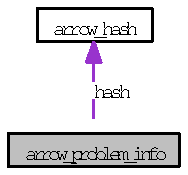
\includegraphics[width=126pt]{structarrow__problem__info__coll__graph}
\end{center}
\end{figure}
\subsection*{Data Fields}
\begin{CompactItemize}
\item 
int $\ast$ \hyperlink{structarrow__problem__info_7c9472312d7057fb9d74eb5579930216}{cost\_\-list}
\item 
int \hyperlink{structarrow__problem__info_54bbdc187af19361072480b45016f171}{cost\_\-list\_\-length}
\item 
int \hyperlink{structarrow__problem__info_46fabcc0ccd3a732cebb014331d4eeb5}{min\_\-cost}
\item 
int \hyperlink{structarrow__problem__info_724060f3be25521cca761899913c2776}{max\_\-cost}
\item 
\hyperlink{structarrow__hash}{arrow\_\-hash} \hyperlink{structarrow__problem__info_d62672139bdce70b23d8c72ecd96ff0d}{hash}
\end{CompactItemize}


\subsection{Detailed Description}
Problem information data structure. 

Definition at line 464 of file common.h.

\subsection{Field Documentation}
\hypertarget{structarrow__problem__info_7c9472312d7057fb9d74eb5579930216}{
\index{arrow\_\-problem\_\-info@{arrow\_\-problem\_\-info}!cost\_\-list@{cost\_\-list}}
\index{cost\_\-list@{cost\_\-list}!arrow_problem_info@{arrow\_\-problem\_\-info}}
\subsubsection[{cost\_\-list}]{\setlength{\rightskip}{0pt plus 5cm}int$\ast$ {\bf arrow\_\-problem\_\-info::cost\_\-list}}}
\label{structarrow__problem__info_7c9472312d7057fb9d74eb5579930216}


sorted list of unique costs from problem. 

Definition at line 466 of file common.h.

Referenced by arrow\_\-balanced\_\-tsp\_\-db(), arrow\_\-balanced\_\-tsp\_\-dt(), arrow\_\-balanced\_\-tsp\_\-dt2(), arrow\_\-balanced\_\-tsp\_\-ib(), arrow\_\-balanced\_\-tsp\_\-ib2(), arrow\_\-balanced\_\-tsp\_\-lb(), arrow\_\-bap\_\-solve(), arrow\_\-bbssp\_\-solve(), arrow\_\-bscssp\_\-solve(), arrow\_\-btsp\_\-solve(), arrow\_\-cbap\_\-solve(), arrow\_\-problem\_\-info\_\-cost\_\-index(), arrow\_\-problem\_\-info\_\-destruct(), arrow\_\-problem\_\-info\_\-get(), baltsp\_\-bounds\_\-tree(), btsp\_\-bounds(), fill\_\-tiers(), and main().\hypertarget{structarrow__problem__info_54bbdc187af19361072480b45016f171}{
\index{arrow\_\-problem\_\-info@{arrow\_\-problem\_\-info}!cost\_\-list\_\-length@{cost\_\-list\_\-length}}
\index{cost\_\-list\_\-length@{cost\_\-list\_\-length}!arrow_problem_info@{arrow\_\-problem\_\-info}}
\subsubsection[{cost\_\-list\_\-length}]{\setlength{\rightskip}{0pt plus 5cm}int {\bf arrow\_\-problem\_\-info::cost\_\-list\_\-length}}}
\label{structarrow__problem__info_54bbdc187af19361072480b45016f171}


length of cost list. 

Definition at line 467 of file common.h.

Referenced by arrow\_\-balanced\_\-tsp\_\-db(), arrow\_\-balanced\_\-tsp\_\-dt(), arrow\_\-balanced\_\-tsp\_\-dt2(), arrow\_\-balanced\_\-tsp\_\-ib(), arrow\_\-balanced\_\-tsp\_\-ib2(), arrow\_\-balanced\_\-tsp\_\-lb(), arrow\_\-baltsp\_\-fun\_\-dt2(), arrow\_\-baltsp\_\-fun\_\-shake(), arrow\_\-bap\_\-solve(), arrow\_\-bbssp\_\-solve(), arrow\_\-bscssp\_\-solve(), arrow\_\-btsp\_\-fun\_\-cbtsp\_\-shake(), arrow\_\-btsp\_\-fun\_\-shake\_\-1(), arrow\_\-btsp\_\-solve(), arrow\_\-cbap\_\-solve(), arrow\_\-problem\_\-info\_\-cost\_\-index(), arrow\_\-problem\_\-info\_\-get(), baltsp\_\-dt2\_\-initialize(), and main().\hypertarget{structarrow__problem__info_d62672139bdce70b23d8c72ecd96ff0d}{
\index{arrow\_\-problem\_\-info@{arrow\_\-problem\_\-info}!hash@{hash}}
\index{hash@{hash}!arrow_problem_info@{arrow\_\-problem\_\-info}}
\subsubsection[{hash}]{\setlength{\rightskip}{0pt plus 5cm}{\bf arrow\_\-hash} {\bf arrow\_\-problem\_\-info::hash}}}
\label{structarrow__problem__info_d62672139bdce70b23d8c72ecd96ff0d}


hash table structure 

Definition at line 470 of file common.h.

Referenced by arrow\_\-problem\_\-info\_\-cost\_\-index(), arrow\_\-problem\_\-info\_\-destruct(), arrow\_\-problem\_\-info\_\-get(), and main().\hypertarget{structarrow__problem__info_724060f3be25521cca761899913c2776}{
\index{arrow\_\-problem\_\-info@{arrow\_\-problem\_\-info}!max\_\-cost@{max\_\-cost}}
\index{max\_\-cost@{max\_\-cost}!arrow_problem_info@{arrow\_\-problem\_\-info}}
\subsubsection[{max\_\-cost}]{\setlength{\rightskip}{0pt plus 5cm}int {\bf arrow\_\-problem\_\-info::max\_\-cost}}}
\label{structarrow__problem__info_724060f3be25521cca761899913c2776}


largest cost in problem. 

Definition at line 469 of file common.h.

Referenced by arrow\_\-balanced\_\-tsp\_\-db(), arrow\_\-balanced\_\-tsp\_\-dt(), arrow\_\-balanced\_\-tsp\_\-dt2(), arrow\_\-balanced\_\-tsp\_\-ib(), arrow\_\-balanced\_\-tsp\_\-ib2(), arrow\_\-balanced\_\-tsp\_\-lb(), arrow\_\-bbssp\_\-solve(), arrow\_\-cbst\_\-mst\_\-solve(), arrow\_\-cbst\_\-solve(), arrow\_\-problem\_\-info\_\-get(), btsp\_\-bounds(), and main().\hypertarget{structarrow__problem__info_46fabcc0ccd3a732cebb014331d4eeb5}{
\index{arrow\_\-problem\_\-info@{arrow\_\-problem\_\-info}!min\_\-cost@{min\_\-cost}}
\index{min\_\-cost@{min\_\-cost}!arrow_problem_info@{arrow\_\-problem\_\-info}}
\subsubsection[{min\_\-cost}]{\setlength{\rightskip}{0pt plus 5cm}int {\bf arrow\_\-problem\_\-info::min\_\-cost}}}
\label{structarrow__problem__info_46fabcc0ccd3a732cebb014331d4eeb5}


smallest cost in problem. 

Definition at line 468 of file common.h.

Referenced by arrow\_\-balanced\_\-tsp\_\-ib(), arrow\_\-problem\_\-info\_\-get(), and main().

The documentation for this struct was generated from the following file:\begin{CompactItemize}
\item 
include/\hyperlink{common_8h}{common.h}\end{CompactItemize}

\hypertarget{structarrow__tsp__lk__params}{
\section{arrow\_\-tsp\_\-lk\_\-params Struct Reference}
\label{structarrow__tsp__lk__params}\index{arrow\_\-tsp\_\-lk\_\-params@{arrow\_\-tsp\_\-lk\_\-params}}
}
LK algorithm parameters.  


{\tt \#include $<$arrow.h$>$}

\subsection*{Data Fields}
\begin{CompactItemize}
\item 
int \hyperlink{structarrow__tsp__lk__params_ec5d500e1f1d7dabbbe0d1aae2abfcf8}{stall\_\-count}
\item 
int \hyperlink{structarrow__tsp__lk__params_9744a2fb89bca6b678fec9a6a17255ea}{kicks}
\item 
int \hyperlink{structarrow__tsp__lk__params_5b724dc268faa478b5b3e14c19abdc2a}{kick\_\-type}
\item 
double \hyperlink{structarrow__tsp__lk__params_22355808165edb6033ca771b88917cf5}{time\_\-bound}
\item 
double \hyperlink{structarrow__tsp__lk__params_36fb446a90e9b4c76702bd93f00357ea}{length\_\-bound}
\item 
int $\ast$ \hyperlink{structarrow__tsp__lk__params_1684519ac0bb6e529707b59f6cd7d528}{initial\_\-tour}
\end{CompactItemize}


\subsection{Detailed Description}
LK algorithm parameters. 

Definition at line 227 of file arrow.h.

\subsection{Field Documentation}
\hypertarget{structarrow__tsp__lk__params_ec5d500e1f1d7dabbbe0d1aae2abfcf8}{
\index{arrow\_\-tsp\_\-lk\_\-params@{arrow\_\-tsp\_\-lk\_\-params}!stall\_\-count@{stall\_\-count}}
\index{stall\_\-count@{stall\_\-count}!arrow_tsp_lk_params@{arrow\_\-tsp\_\-lk\_\-params}}
\subsubsection{\setlength{\rightskip}{0pt plus 5cm}int {\bf arrow\_\-tsp\_\-lk\_\-params::stall\_\-count}}}
\label{structarrow__tsp__lk__params_ec5d500e1f1d7dabbbe0d1aae2abfcf8}


the max number of 4-swap kicks to perform without making progress 

Definition at line 229 of file arrow.h.\hypertarget{structarrow__tsp__lk__params_9744a2fb89bca6b678fec9a6a17255ea}{
\index{arrow\_\-tsp\_\-lk\_\-params@{arrow\_\-tsp\_\-lk\_\-params}!kicks@{kicks}}
\index{kicks@{kicks}!arrow_tsp_lk_params@{arrow\_\-tsp\_\-lk\_\-params}}
\subsubsection{\setlength{\rightskip}{0pt plus 5cm}int {\bf arrow\_\-tsp\_\-lk\_\-params::kicks}}}
\label{structarrow__tsp__lk__params_9744a2fb89bca6b678fec9a6a17255ea}


the number of 4-swap kicks to perform 

Definition at line 231 of file arrow.h.\hypertarget{structarrow__tsp__lk__params_5b724dc268faa478b5b3e14c19abdc2a}{
\index{arrow\_\-tsp\_\-lk\_\-params@{arrow\_\-tsp\_\-lk\_\-params}!kick\_\-type@{kick\_\-type}}
\index{kick\_\-type@{kick\_\-type}!arrow_tsp_lk_params@{arrow\_\-tsp\_\-lk\_\-params}}
\subsubsection{\setlength{\rightskip}{0pt plus 5cm}int {\bf arrow\_\-tsp\_\-lk\_\-params::kick\_\-type}}}
\label{structarrow__tsp__lk__params_5b724dc268faa478b5b3e14c19abdc2a}


the type of kick: one of CC\_\-LK\_\-RANDOM\_\-KICK, CC\_\-LK\_\-GEOMETRIC\_\-KICK, or CC\_\-LK\_\-CLOSE\_\-KICK; see Concorde documentation for more info 

Definition at line 232 of file arrow.h.\hypertarget{structarrow__tsp__lk__params_22355808165edb6033ca771b88917cf5}{
\index{arrow\_\-tsp\_\-lk\_\-params@{arrow\_\-tsp\_\-lk\_\-params}!time\_\-bound@{time\_\-bound}}
\index{time\_\-bound@{time\_\-bound}!arrow_tsp_lk_params@{arrow\_\-tsp\_\-lk\_\-params}}
\subsubsection{\setlength{\rightskip}{0pt plus 5cm}double {\bf arrow\_\-tsp\_\-lk\_\-params::time\_\-bound}}}
\label{structarrow__tsp__lk__params_22355808165edb6033ca771b88917cf5}


stop after this running time reached; set to 0 to have no time bound, must be positive 

Definition at line 235 of file arrow.h.\hypertarget{structarrow__tsp__lk__params_36fb446a90e9b4c76702bd93f00357ea}{
\index{arrow\_\-tsp\_\-lk\_\-params@{arrow\_\-tsp\_\-lk\_\-params}!length\_\-bound@{length\_\-bound}}
\index{length\_\-bound@{length\_\-bound}!arrow_tsp_lk_params@{arrow\_\-tsp\_\-lk\_\-params}}
\subsubsection{\setlength{\rightskip}{0pt plus 5cm}double {\bf arrow\_\-tsp\_\-lk\_\-params::length\_\-bound}}}
\label{structarrow__tsp__lk__params_36fb446a90e9b4c76702bd93f00357ea}


stop after finding tour of this length; must be non-negative 

Definition at line 237 of file arrow.h.\hypertarget{structarrow__tsp__lk__params_1684519ac0bb6e529707b59f6cd7d528}{
\index{arrow\_\-tsp\_\-lk\_\-params@{arrow\_\-tsp\_\-lk\_\-params}!initial\_\-tour@{initial\_\-tour}}
\index{initial\_\-tour@{initial\_\-tour}!arrow_tsp_lk_params@{arrow\_\-tsp\_\-lk\_\-params}}
\subsubsection{\setlength{\rightskip}{0pt plus 5cm}int$\ast$ {\bf arrow\_\-tsp\_\-lk\_\-params::initial\_\-tour}}}
\label{structarrow__tsp__lk__params_1684519ac0bb6e529707b59f6cd7d528}


initial tour (may be NULL) 

Definition at line 239 of file arrow.h.

The documentation for this struct was generated from the following file:\begin{CompactItemize}
\item 
lib/\hyperlink{arrow_8h}{arrow.h}\end{CompactItemize}

\hypertarget{structarrow__tsp__result}{
\section{arrow\_\-tsp\_\-result Struct Reference}
\label{structarrow__tsp__result}\index{arrow\_\-tsp\_\-result@{arrow\_\-tsp\_\-result}}
}
TSP result (including result from LK heuristic).  


{\tt \#include $<$arrow.h$>$}

\subsection*{Data Fields}
\begin{CompactItemize}
\item 
int \hyperlink{structarrow__tsp__result_b85143df6ecc70032db7411a1aa3192a}{found\_\-tour}
\item 
double \hyperlink{structarrow__tsp__result_93a335ce86270dd455185d22ea5fd4ab}{tour\_\-length}
\item 
int $\ast$ \hyperlink{structarrow__tsp__result_48433b03146d6ca3423a555ea2139d52}{tour}
\item 
double \hyperlink{structarrow__tsp__result_82ea7aa0320d932892602d34339a9276}{total\_\-time}
\end{CompactItemize}


\subsection{Detailed Description}
TSP result (including result from LK heuristic). 

Definition at line 216 of file arrow.h.

\subsection{Field Documentation}
\hypertarget{structarrow__tsp__result_b85143df6ecc70032db7411a1aa3192a}{
\index{arrow\_\-tsp\_\-result@{arrow\_\-tsp\_\-result}!found\_\-tour@{found\_\-tour}}
\index{found\_\-tour@{found\_\-tour}!arrow_tsp_result@{arrow\_\-tsp\_\-result}}
\subsubsection{\setlength{\rightskip}{0pt plus 5cm}int {\bf arrow\_\-tsp\_\-result::found\_\-tour}}}
\label{structarrow__tsp__result_b85143df6ecc70032db7411a1aa3192a}


true if a tour was found, false otherwise 

Definition at line 218 of file arrow.h.

Referenced by arrow\_\-tsp\_\-exact\_\-solve(), and arrow\_\-tsp\_\-result\_\-init().\hypertarget{structarrow__tsp__result_93a335ce86270dd455185d22ea5fd4ab}{
\index{arrow\_\-tsp\_\-result@{arrow\_\-tsp\_\-result}!tour\_\-length@{tour\_\-length}}
\index{tour\_\-length@{tour\_\-length}!arrow_tsp_result@{arrow\_\-tsp\_\-result}}
\subsubsection{\setlength{\rightskip}{0pt plus 5cm}double {\bf arrow\_\-tsp\_\-result::tour\_\-length}}}
\label{structarrow__tsp__result_93a335ce86270dd455185d22ea5fd4ab}


tour length 

Definition at line 219 of file arrow.h.

Referenced by arrow\_\-tsp\_\-exact\_\-solve(), and arrow\_\-tsp\_\-result\_\-init().\hypertarget{structarrow__tsp__result_48433b03146d6ca3423a555ea2139d52}{
\index{arrow\_\-tsp\_\-result@{arrow\_\-tsp\_\-result}!tour@{tour}}
\index{tour@{tour}!arrow_tsp_result@{arrow\_\-tsp\_\-result}}
\subsubsection{\setlength{\rightskip}{0pt plus 5cm}int$\ast$ {\bf arrow\_\-tsp\_\-result::tour}}}
\label{structarrow__tsp__result_48433b03146d6ca3423a555ea2139d52}


tour that was found in node-node format 

Definition at line 220 of file arrow.h.

Referenced by arrow\_\-tsp\_\-exact\_\-solve(), arrow\_\-tsp\_\-result\_\-destruct(), and arrow\_\-tsp\_\-result\_\-init().\hypertarget{structarrow__tsp__result_82ea7aa0320d932892602d34339a9276}{
\index{arrow\_\-tsp\_\-result@{arrow\_\-tsp\_\-result}!total\_\-time@{total\_\-time}}
\index{total\_\-time@{total\_\-time}!arrow_tsp_result@{arrow\_\-tsp\_\-result}}
\subsubsection{\setlength{\rightskip}{0pt plus 5cm}double {\bf arrow\_\-tsp\_\-result::total\_\-time}}}
\label{structarrow__tsp__result_82ea7aa0320d932892602d34339a9276}


total time 

Definition at line 221 of file arrow.h.

Referenced by arrow\_\-tsp\_\-exact\_\-solve(), and arrow\_\-tsp\_\-result\_\-init().

The documentation for this struct was generated from the following file:\begin{CompactItemize}
\item 
lib/\hyperlink{arrow_8h}{arrow.h}\end{CompactItemize}

\hypertarget{structbasic__data}{
\section{basic\_\-data Struct Reference}
\label{structbasic__data}\index{basic\_\-data@{basic\_\-data}}
}
Concorde userdat structure for basic cost matrix function.  


\subsection*{Data Fields}
\begin{CompactItemize}
\item 
CCdatagroup $\ast$ \hyperlink{structbasic__data_02bf35a1e012cfcd2a2e39fb5cf0b5aa}{dat}
\item 
int \hyperlink{structbasic__data_6ca72860561070179323aeacf49c81d8}{delta}
\end{CompactItemize}


\subsection{Detailed Description}
Concorde userdat structure for basic cost matrix function. 

Definition at line 178 of file btsp\_\-fun.c.

\subsection{Field Documentation}
\hypertarget{structbasic__data_02bf35a1e012cfcd2a2e39fb5cf0b5aa}{
\index{basic\_\-data@{basic\_\-data}!dat@{dat}}
\index{dat@{dat}!basic_data@{basic\_\-data}}
\subsubsection{\setlength{\rightskip}{0pt plus 5cm}CCdatagroup$\ast$ {\bf basic\_\-data::dat}}}
\label{structbasic__data_02bf35a1e012cfcd2a2e39fb5cf0b5aa}


existing Concorde data structure 

Definition at line 180 of file btsp\_\-fun.c.

Referenced by basic\_\-edgelen(), and basic\_\-shallow\_\-apply().\hypertarget{structbasic__data_6ca72860561070179323aeacf49c81d8}{
\index{basic\_\-data@{basic\_\-data}!delta@{delta}}
\index{delta@{delta}!basic_data@{basic\_\-data}}
\subsubsection{\setlength{\rightskip}{0pt plus 5cm}int {\bf basic\_\-data::delta}}}
\label{structbasic__data_6ca72860561070179323aeacf49c81d8}


delta value 

Definition at line 181 of file btsp\_\-fun.c.

Referenced by basic\_\-shallow\_\-apply().

The documentation for this struct was generated from the following file:\begin{CompactItemize}
\item 
lib/\hyperlink{btsp__fun_8c}{btsp\_\-fun.c}\end{CompactItemize}

\hypertarget{structconstrained__data}{
\section{constrained\_\-data Struct Reference}
\label{structconstrained__data}\index{constrained\_\-data@{constrained\_\-data}}
}
Concorde userdat structure for constrained cost matrix function.  


\subsection*{Data Fields}
\begin{CompactItemize}
\item 
CCdatagroup $\ast$ \hyperlink{structconstrained__data_517c13548dbd3645f85fc59b9aaa5f5a}{dat}
\item 
int \hyperlink{structconstrained__data_113c60c7266cd5834238e7dd325899fa}{infinity}
\item 
int \hyperlink{structconstrained__data_1f33c1fc7b0fdcb2771167f061ff4724}{delta}
\end{CompactItemize}


\subsection{Detailed Description}
Concorde userdat structure for constrained cost matrix function. 

Definition at line 187 of file btsp\_\-fun.c.

\subsection{Field Documentation}
\hypertarget{structconstrained__data_517c13548dbd3645f85fc59b9aaa5f5a}{
\index{constrained\_\-data@{constrained\_\-data}!dat@{dat}}
\index{dat@{dat}!constrained_data@{constrained\_\-data}}
\subsubsection{\setlength{\rightskip}{0pt plus 5cm}CCdatagroup$\ast$ {\bf constrained\_\-data::dat}}}
\label{structconstrained__data_517c13548dbd3645f85fc59b9aaa5f5a}


existing Concorde data structure 

Definition at line 189 of file btsp\_\-fun.c.

Referenced by constrained\_\-edgelen(), and constrained\_\-shallow\_\-apply().\hypertarget{structconstrained__data_113c60c7266cd5834238e7dd325899fa}{
\index{constrained\_\-data@{constrained\_\-data}!infinity@{infinity}}
\index{infinity@{infinity}!constrained_data@{constrained\_\-data}}
\subsubsection{\setlength{\rightskip}{0pt plus 5cm}int {\bf constrained\_\-data::infinity}}}
\label{structconstrained__data_113c60c7266cd5834238e7dd325899fa}


value to use for \char`\"{}infinity\char`\"{} 

Definition at line 190 of file btsp\_\-fun.c.

Referenced by constrained\_\-edgelen(), and constrained\_\-shallow\_\-apply().\hypertarget{structconstrained__data_1f33c1fc7b0fdcb2771167f061ff4724}{
\index{constrained\_\-data@{constrained\_\-data}!delta@{delta}}
\index{delta@{delta}!constrained_data@{constrained\_\-data}}
\subsubsection{\setlength{\rightskip}{0pt plus 5cm}int {\bf constrained\_\-data::delta}}}
\label{structconstrained__data_1f33c1fc7b0fdcb2771167f061ff4724}


delta value 

Definition at line 191 of file btsp\_\-fun.c.

Referenced by constrained\_\-shallow\_\-apply().

The documentation for this struct was generated from the following file:\begin{CompactItemize}
\item 
lib/\hyperlink{btsp__fun_8c}{btsp\_\-fun.c}\end{CompactItemize}

\hypertarget{structconstrained__shake__data}{
\section{constrained\_\-shake\_\-data Struct Reference}
\label{structconstrained__shake__data}\index{constrained\_\-shake\_\-data@{constrained\_\-shake\_\-data}}
}
Concorde userdat structure for constrained shake cost matrix function.  


Collaboration diagram for constrained\_\-shake\_\-data:\subsection*{Data Fields}
\begin{CompactItemize}
\item 
\hyperlink{structarrow__problem}{arrow\_\-problem} $\ast$ \hyperlink{structconstrained__shake__data_ae6de8c84cb5dc65aae992effa7c2763}{problem}
\item 
\hyperlink{structarrow__problem__info}{arrow\_\-problem\_\-info} $\ast$ \hyperlink{structconstrained__shake__data_d9b2d3116046f50437d023ac9bfcd51f}{info}
\item 
int \hyperlink{structconstrained__shake__data_76a13ad58e4ad8c74270ce8b05765ff9}{rand\_\-min}
\item 
int \hyperlink{structconstrained__shake__data_39972f2868c566a04f200957d9ad0c3f}{rand\_\-max}
\item 
int \hyperlink{structconstrained__shake__data_0114e4db38ea88cd199781d7ba97a44b}{random\_\-list\_\-length}
\item 
int \hyperlink{structconstrained__shake__data_ba0c33ec57d7f977911088e41b48c606}{infinity}
\end{CompactItemize}


\subsection{Detailed Description}
Concorde userdat structure for constrained shake cost matrix function. 

Definition at line 198 of file btsp\_\-fun.c.

\subsection{Field Documentation}
\hypertarget{structconstrained__shake__data_ae6de8c84cb5dc65aae992effa7c2763}{
\index{constrained\_\-shake\_\-data@{constrained\_\-shake\_\-data}!problem@{problem}}
\index{problem@{problem}!constrained_shake_data@{constrained\_\-shake\_\-data}}
\subsubsection{\setlength{\rightskip}{0pt plus 5cm}{\bf arrow\_\-problem}$\ast$ {\bf constrained\_\-shake\_\-data::problem}}}
\label{structconstrained__shake__data_ae6de8c84cb5dc65aae992effa7c2763}


original problem data 

Definition at line 200 of file btsp\_\-fun.c.

Referenced by arrow\_\-btsp\_\-fun\_\-constrained\_\-shake().\hypertarget{structconstrained__shake__data_d9b2d3116046f50437d023ac9bfcd51f}{
\index{constrained\_\-shake\_\-data@{constrained\_\-shake\_\-data}!info@{info}}
\index{info@{info}!constrained_shake_data@{constrained\_\-shake\_\-data}}
\subsubsection{\setlength{\rightskip}{0pt plus 5cm}{\bf arrow\_\-problem\_\-info}$\ast$ {\bf constrained\_\-shake\_\-data::info}}}
\label{structconstrained__shake__data_d9b2d3116046f50437d023ac9bfcd51f}


original problem info 

Definition at line 201 of file btsp\_\-fun.c.

Referenced by arrow\_\-btsp\_\-fun\_\-constrained\_\-shake(), and constrained\_\-shake\_\-deep\_\-apply().\hypertarget{structconstrained__shake__data_76a13ad58e4ad8c74270ce8b05765ff9}{
\index{constrained\_\-shake\_\-data@{constrained\_\-shake\_\-data}!rand\_\-min@{rand\_\-min}}
\index{rand\_\-min@{rand\_\-min}!constrained_shake_data@{constrained\_\-shake\_\-data}}
\subsubsection{\setlength{\rightskip}{0pt plus 5cm}int {\bf constrained\_\-shake\_\-data::rand\_\-min}}}
\label{structconstrained__shake__data_76a13ad58e4ad8c74270ce8b05765ff9}


smallest random number to generate 

Definition at line 202 of file btsp\_\-fun.c.

Referenced by arrow\_\-btsp\_\-fun\_\-constrained\_\-shake(), and constrained\_\-shake\_\-deep\_\-apply().\hypertarget{structconstrained__shake__data_39972f2868c566a04f200957d9ad0c3f}{
\index{constrained\_\-shake\_\-data@{constrained\_\-shake\_\-data}!rand\_\-max@{rand\_\-max}}
\index{rand\_\-max@{rand\_\-max}!constrained_shake_data@{constrained\_\-shake\_\-data}}
\subsubsection{\setlength{\rightskip}{0pt plus 5cm}int {\bf constrained\_\-shake\_\-data::rand\_\-max}}}
\label{structconstrained__shake__data_39972f2868c566a04f200957d9ad0c3f}


largest random number to generate 

Definition at line 203 of file btsp\_\-fun.c.

Referenced by arrow\_\-btsp\_\-fun\_\-constrained\_\-shake(), and constrained\_\-shake\_\-deep\_\-apply().\hypertarget{structconstrained__shake__data_0114e4db38ea88cd199781d7ba97a44b}{
\index{constrained\_\-shake\_\-data@{constrained\_\-shake\_\-data}!random\_\-list\_\-length@{random\_\-list\_\-length}}
\index{random\_\-list\_\-length@{random\_\-list\_\-length}!constrained_shake_data@{constrained\_\-shake\_\-data}}
\subsubsection{\setlength{\rightskip}{0pt plus 5cm}int {\bf constrained\_\-shake\_\-data::random\_\-list\_\-length}}}
\label{structconstrained__shake__data_0114e4db38ea88cd199781d7ba97a44b}


the number of random numbers in list 

Definition at line 204 of file btsp\_\-fun.c.\hypertarget{structconstrained__shake__data_ba0c33ec57d7f977911088e41b48c606}{
\index{constrained\_\-shake\_\-data@{constrained\_\-shake\_\-data}!infinity@{infinity}}
\index{infinity@{infinity}!constrained_shake_data@{constrained\_\-shake\_\-data}}
\subsubsection{\setlength{\rightskip}{0pt plus 5cm}int {\bf constrained\_\-shake\_\-data::infinity}}}
\label{structconstrained__shake__data_ba0c33ec57d7f977911088e41b48c606}


value to use for \char`\"{}infinity\char`\"{} 

Definition at line 205 of file btsp\_\-fun.c.

Referenced by arrow\_\-btsp\_\-fun\_\-constrained\_\-shake(), and constrained\_\-shake\_\-deep\_\-apply().

The documentation for this struct was generated from the following file:\begin{CompactItemize}
\item 
lib/\hyperlink{btsp__fun_8c}{btsp\_\-fun.c}\end{CompactItemize}

\chapter{File Documentation}
\hypertarget{bin_22mb_8c}{
\section{bin/2mb.c File Reference}
\label{bin_22mb_8c}\index{bin/2mb.c@{bin/2mb.c}}
}
2-Max Bound solver. 

{\tt \#include \char`\"{}arrow.h\char`\"{}}\par


Include dependency graph for 2mb.c:\subsection*{Defines}
\begin{CompactItemize}
\item 
\#define \hyperlink{bin_22mb_8c_9b58b2c4af931c8486a986c9deca40f5}{NUM\_\-OPTS}~2
\end{CompactItemize}
\subsection*{Functions}
\begin{CompactItemize}
\item 
int \hyperlink{bin_22mb_8c_0ddf1224851353fc92bfbff6f499fa97}{main} (int argc, char $\ast$argv\mbox{[}$\,$\mbox{]})
\end{CompactItemize}
\subsection*{Variables}
\begin{CompactItemize}
\item 
char $\ast$ \hyperlink{bin_22mb_8c_289c5900d90626d909f0a85d5a0ed61d}{program\_\-name}
\item 
char $\ast$ \hyperlink{bin_22mb_8c_a4f3a15de34c409bdec6ceacf93078ed}{input\_\-file} = NULL
\item 
char $\ast$ \hyperlink{bin_22mb_8c_bf4e392494984c6ef8259268eb1fe421}{xml\_\-file} = NULL
\item 
\hyperlink{structarrow__option}{arrow\_\-option} \hyperlink{bin_22mb_8c_cea6a9709d519c143f30db401a0d0c72}{options} \mbox{[}NUM\_\-OPTS\mbox{]}
\item 
char $\ast$ \hyperlink{bin_22mb_8c_3aad16fd4bea1b9717f232ea75ad6449}{desc} = \char`\"{}2-Max Bound solver\char`\"{}
\item 
char $\ast$ \hyperlink{bin_22mb_8c_adebe2487a2c5240ab6cd02c83add0bf}{usage} = \char`\"{}-i tsplib.tsp \mbox{[}\hyperlink{histogram__data_8c_cea6a9709d519c143f30db401a0d0c72}{options}\mbox{]} \char`\"{}
\end{CompactItemize}


\subsection{Detailed Description}
2-Max Bound solver. 

Solves the 2-max bound (2MB) on the given input file.

\begin{Desc}
\item[Author:]John LaRusic \end{Desc}


Definition in file \hyperlink{bin_22mb_8c-source}{2mb.c}.

\subsection{Define Documentation}
\hypertarget{bin_22mb_8c_9b58b2c4af931c8486a986c9deca40f5}{
\index{bin/2mb.c@{bin/2mb.c}!NUM\_\-OPTS@{NUM\_\-OPTS}}
\index{NUM\_\-OPTS@{NUM\_\-OPTS}!bin/2mb.c@{bin/2mb.c}}
\subsubsection{\setlength{\rightskip}{0pt plus 5cm}\#define NUM\_\-OPTS~2}}
\label{bin_22mb_8c_9b58b2c4af931c8486a986c9deca40f5}




Definition at line 17 of file 2mb.c.

Referenced by main().

\subsection{Function Documentation}
\hypertarget{bin_22mb_8c_0ddf1224851353fc92bfbff6f499fa97}{
\index{bin/2mb.c@{bin/2mb.c}!main@{main}}
\index{main@{main}!bin/2mb.c@{bin/2mb.c}}
\subsubsection{\setlength{\rightskip}{0pt plus 5cm}int main (int {\em argc}, \/  char $\ast$ {\em argv}\mbox{[}$\,$\mbox{]})}}
\label{bin_22mb_8c_0ddf1224851353fc92bfbff6f499fa97}




Definition at line 30 of file 2mb.c.

References arrow\_\-2mb\_\-solve(), ARROW\_\-FAILURE, arrow\_\-options\_\-parse(), arrow\_\-print\_\-error, arrow\_\-problem\_\-destruct(), arrow\_\-problem\_\-read(), ARROW\_\-SUCCESS, arrow\_\-util\_\-print\_\-program\_\-args(), desc, input\_\-file, NUM\_\-OPTS, arrow\_\-bound\_\-result::obj\_\-value, arrow\_\-bound\_\-result::total\_\-time, usage, and xml\_\-file.

\subsection{Variable Documentation}
\hypertarget{bin_22mb_8c_3aad16fd4bea1b9717f232ea75ad6449}{
\index{bin/2mb.c@{bin/2mb.c}!desc@{desc}}
\index{desc@{desc}!bin/2mb.c@{bin/2mb.c}}
\subsubsection{\setlength{\rightskip}{0pt plus 5cm}char$\ast$ {\bf desc} = \char`\"{}2-Max Bound solver\char`\"{}}}
\label{bin_22mb_8c_3aad16fd4bea1b9717f232ea75ad6449}




Definition at line 25 of file 2mb.c.

Referenced by main().\hypertarget{bin_22mb_8c_a4f3a15de34c409bdec6ceacf93078ed}{
\index{bin/2mb.c@{bin/2mb.c}!input\_\-file@{input\_\-file}}
\index{input\_\-file@{input\_\-file}!bin/2mb.c@{bin/2mb.c}}
\subsubsection{\setlength{\rightskip}{0pt plus 5cm}char$\ast$ {\bf input\_\-file} = NULL}}
\label{bin_22mb_8c_a4f3a15de34c409bdec6ceacf93078ed}


Given input TSPLIB file 

Definition at line 13 of file 2mb.c.

Referenced by main(), and read\_\-args().\hypertarget{bin_22mb_8c_cea6a9709d519c143f30db401a0d0c72}{
\index{bin/2mb.c@{bin/2mb.c}!options@{options}}
\index{options@{options}!bin/2mb.c@{bin/2mb.c}}
\subsubsection{\setlength{\rightskip}{0pt plus 5cm}{\bf arrow\_\-option} {\bf options}\mbox{[}NUM\_\-OPTS\mbox{]}}}
\label{bin_22mb_8c_cea6a9709d519c143f30db401a0d0c72}


\textbf{Initial value:}

\begin{Code}\begin{verbatim} 
{
    {'i', "input", "TSPLIB input file", 
        ARROW_OPTION_STRING, &input_file, ARROW_TRUE, ARROW_TRUE},
    {'x', "xml", "File to write XML output to",
        ARROW_OPTION_STRING, &xml_file, ARROW_FALSE, ARROW_TRUE}
}
\end{verbatim}
\end{Code}


Definition at line 18 of file 2mb.c.\hypertarget{bin_22mb_8c_289c5900d90626d909f0a85d5a0ed61d}{
\index{bin/2mb.c@{bin/2mb.c}!program\_\-name@{program\_\-name}}
\index{program\_\-name@{program\_\-name}!bin/2mb.c@{bin/2mb.c}}
\subsubsection{\setlength{\rightskip}{0pt plus 5cm}char$\ast$ {\bf program\_\-name}}}
\label{bin_22mb_8c_289c5900d90626d909f0a85d5a0ed61d}


Program name 

Definition at line 12 of file 2mb.c.

Referenced by main(), print\_\-help(), print\_\-usage(), and print\_\-version().\hypertarget{bin_22mb_8c_adebe2487a2c5240ab6cd02c83add0bf}{
\index{bin/2mb.c@{bin/2mb.c}!usage@{usage}}
\index{usage@{usage}!bin/2mb.c@{bin/2mb.c}}
\subsubsection{\setlength{\rightskip}{0pt plus 5cm}char$\ast$ {\bf usage} = \char`\"{}-i tsplib.tsp \mbox{[}{\bf options}\mbox{]} \char`\"{}}}
\label{bin_22mb_8c_adebe2487a2c5240ab6cd02c83add0bf}




Definition at line 26 of file 2mb.c.

Referenced by main().\hypertarget{bin_22mb_8c_bf4e392494984c6ef8259268eb1fe421}{
\index{bin/2mb.c@{bin/2mb.c}!xml\_\-file@{xml\_\-file}}
\index{xml\_\-file@{xml\_\-file}!bin/2mb.c@{bin/2mb.c}}
\subsubsection{\setlength{\rightskip}{0pt plus 5cm}char$\ast$ {\bf xml\_\-file} = NULL}}
\label{bin_22mb_8c_bf4e392494984c6ef8259268eb1fe421}




Definition at line 14 of file 2mb.c.

Referenced by main().
\hypertarget{lib_22mb_8c}{
\section{lib/2mb.c File Reference}
\label{lib_22mb_8c}\index{lib/2mb.c@{lib/2mb.c}}
}
2-max bound implemenation. 

{\tt \#include \char`\"{}arrow.h\char`\"{}}\par
\subsection*{Functions}
\begin{CompactItemize}
\item 
int \hyperlink{lib_22mb_8c_a3ac7f6280e1eaea38fafbe78375b13f}{arrow\_\-2mb\_\-solve} (\hyperlink{structarrow__problem}{arrow\_\-problem} $\ast$problem, \hyperlink{structarrow__bound__result}{arrow\_\-bound\_\-result} $\ast$result)
\begin{CompactList}\small\item\em Solves the 2-max bound (2MB) on the given problem. \item\end{CompactList}\end{CompactItemize}


\subsection{Detailed Description}
2-max bound implemenation. 

Implemenation of the 2-max bound (2MB) used as a lower bound for the Bottleneck TSP objective value.

\begin{Desc}
\item[Author:]John LaRusic \end{Desc}


Definition in file \hyperlink{lib_22mb_8c-source}{2mb.c}.

\subsection{Function Documentation}
\hypertarget{lib_22mb_8c_a3ac7f6280e1eaea38fafbe78375b13f}{
\index{lib/2mb.c@{lib/2mb.c}!arrow\_\-2mb\_\-solve@{arrow\_\-2mb\_\-solve}}
\index{arrow\_\-2mb\_\-solve@{arrow\_\-2mb\_\-solve}!lib/2mb.c@{lib/2mb.c}}
\subsubsection{\setlength{\rightskip}{0pt plus 5cm}int arrow\_\-2mb\_\-solve ({\bf arrow\_\-problem} $\ast$ {\em problem}, \/  {\bf arrow\_\-bound\_\-result} $\ast$ {\em result})}}
\label{lib_22mb_8c_a3ac7f6280e1eaea38fafbe78375b13f}


Solves the 2-max bound (2MB) on the given problem. 

\begin{Desc}
\item[Parameters:]
\begin{description}
\item[{\em problem}]\mbox{[}in\mbox{]} problem data \item[{\em result}]\mbox{[}out\mbox{]} 2MB solution \end{description}
\end{Desc}


Definition at line 16 of file 2mb.c.

References ARROW\_\-SUCCESS, arrow\_\-util\_\-zeit(), arrow\_\-problem::get\_\-cost, max(), arrow\_\-bound\_\-result::obj\_\-value, arrow\_\-problem::size, arrow\_\-problem::symmetric, and arrow\_\-bound\_\-result::total\_\-time.

Referenced by main().
\hypertarget{abtsp_8c}{
\section{bin/abtsp.c File Reference}
\label{abtsp_8c}\index{bin/abtsp.c@{bin/abtsp.c}}
}
Asymmetric Bottleneck TSP heuristic. 

{\tt \#include \char`\"{}arrow.h\char`\"{}}\par
\subsection*{Defines}
\begin{CompactItemize}
\item 
\#define \hyperlink{abtsp_8c_9b58b2c4af931c8486a986c9deca40f5}{NUM\_\-OPTS}~12
\item 
\#define \hyperlink{abtsp_8c_ceebcce8f411269df7b99e78247d7497}{SOLVE\_\-STEPS}~1
\end{CompactItemize}
\subsection*{Functions}
\begin{CompactItemize}
\item 
int \hyperlink{abtsp_8c_0ddf1224851353fc92bfbff6f499fa97}{main} (int argc, char $\ast$argv\mbox{[}$\,$\mbox{]})
\end{CompactItemize}
\subsection*{Variables}
\begin{CompactItemize}
\item 
char $\ast$ \hyperlink{abtsp_8c_a4f3a15de34c409bdec6ceacf93078ed}{input\_\-file} = NULL
\item 
char $\ast$ \hyperlink{abtsp_8c_bf4e392494984c6ef8259268eb1fe421}{xml\_\-file} = NULL
\item 
char $\ast$ \hyperlink{abtsp_8c_b818a82f867be75d7c4d92d792b0943e}{tour\_\-file} = NULL
\item 
int \hyperlink{abtsp_8c_e6a9db0fe5c8a0407d62dec2f7a14959}{random\_\-restarts} = -1
\item 
int \hyperlink{abtsp_8c_a1641a28cf3ea572a56763e84518c17b}{stall\_\-count} = -1
\item 
int \hyperlink{abtsp_8c_b8f057ba1ad6b7f0c46f8140b25b3467}{kicks} = -1
\item 
int \hyperlink{abtsp_8c_5f4aa75866b44d2dc5f30ee0175d44ff}{confirm\_\-sol} = ARROW\_\-FALSE
\item 
int \hyperlink{abtsp_8c_502a0aac74d070b870b1c096d9d8520d}{supress\_\-ebst} = ARROW\_\-FALSE
\item 
int \hyperlink{abtsp_8c_ed48edf71a0207dcdec06e399c24df88}{find\_\-short\_\-tour} = ARROW\_\-FALSE
\item 
int \hyperlink{abtsp_8c_ed7394fd8e0c2796b26b9654fd10fd9d}{lower\_\-bound} = -1
\item 
int \hyperlink{abtsp_8c_f5a34eb1d01ffd792adcadc9627ffcb8}{upper\_\-bound} = INT\_\-MAX
\item 
int \hyperlink{abtsp_8c_227b7ec968925f365b96a92ace419c56}{basic\_\-attempts} = ARROW\_\-DEFAULT\_\-BASIC\_\-ATTEMPTS
\item 
\hyperlink{structarrow__option}{arrow\_\-option} \hyperlink{abtsp_8c_cea6a9709d519c143f30db401a0d0c72}{options} \mbox{[}NUM\_\-OPTS\mbox{]}
\item 
char $\ast$ \hyperlink{abtsp_8c_3aad16fd4bea1b9717f232ea75ad6449}{desc} = \char`\"{}Bottleneck traveling salesman problem (BTSP) solver\char`\"{}
\item 
char $\ast$ \hyperlink{abtsp_8c_adebe2487a2c5240ab6cd02c83add0bf}{usage} = \char`\"{}-i tsplib.tsp \mbox{[}\hyperlink{subproblem_8c_cea6a9709d519c143f30db401a0d0c72}{options}\mbox{]}\char`\"{}
\end{CompactItemize}


\subsection{Detailed Description}
Asymmetric Bottleneck TSP heuristic. 

Runs the Bottleneck TSP heuristic on the given asymmetric input file.

\begin{Desc}
\item[Author:]John LaRusic \end{Desc}


Definition in file \hyperlink{abtsp_8c-source}{abtsp.c}.

\subsection{Define Documentation}
\hypertarget{abtsp_8c_9b58b2c4af931c8486a986c9deca40f5}{
\index{abtsp.c@{abtsp.c}!NUM\_\-OPTS@{NUM\_\-OPTS}}
\index{NUM\_\-OPTS@{NUM\_\-OPTS}!abtsp.c@{abtsp.c}}
\subsubsection{\setlength{\rightskip}{0pt plus 5cm}\#define NUM\_\-OPTS~12}}
\label{abtsp_8c_9b58b2c4af931c8486a986c9deca40f5}




Definition at line 26 of file abtsp.c.\hypertarget{abtsp_8c_ceebcce8f411269df7b99e78247d7497}{
\index{abtsp.c@{abtsp.c}!SOLVE\_\-STEPS@{SOLVE\_\-STEPS}}
\index{SOLVE\_\-STEPS@{SOLVE\_\-STEPS}!abtsp.c@{abtsp.c}}
\subsubsection{\setlength{\rightskip}{0pt plus 5cm}\#define SOLVE\_\-STEPS~1}}
\label{abtsp_8c_ceebcce8f411269df7b99e78247d7497}




Referenced by main().

\subsection{Function Documentation}
\hypertarget{abtsp_8c_0ddf1224851353fc92bfbff6f499fa97}{
\index{abtsp.c@{abtsp.c}!main@{main}}
\index{main@{main}!abtsp.c@{abtsp.c}}
\subsubsection{\setlength{\rightskip}{0pt plus 5cm}int main (int {\em argc}, \/  char $\ast$ {\em argv}\mbox{[}$\,$\mbox{]})}}
\label{abtsp_8c_0ddf1224851353fc92bfbff6f499fa97}




Definition at line 61 of file abtsp.c.

References arrow\_\-btsp\_\-fun\_\-basic\_\-atsp(), arrow\_\-btsp\_\-fun\_\-destruct(), arrow\_\-btsp\_\-params\_\-destruct(), arrow\_\-btsp\_\-params\_\-init(), arrow\_\-btsp\_\-result\_\-destruct(), arrow\_\-btsp\_\-result\_\-init(), arrow\_\-btsp\_\-solve(), ARROW\_\-BTSP\_\-SOLVE\_\-PLAN\_\-BASIC, arrow\_\-debug, ARROW\_\-FAILURE, ARROW\_\-FALSE, arrow\_\-options\_\-parse(), arrow\_\-print\_\-error, arrow\_\-problem\_\-abtsp\_\-to\_\-sbtsp(), arrow\_\-problem\_\-destruct(), arrow\_\-problem\_\-info\_\-get(), arrow\_\-problem\_\-read(), ARROW\_\-SUCCESS, ARROW\_\-TRUE, arrow\_\-tsp\_\-lk\_\-params\_\-destruct(), arrow\_\-tsp\_\-lk\_\-params\_\-init(), arrow\_\-util\_\-create\_\-int\_\-array(), arrow\_\-util\_\-print\_\-program\_\-args(), arrow\_\-util\_\-sbtsp\_\-to\_\-abstp\_\-tour(), arrow\_\-util\_\-write\_\-tour(), arrow\_\-util\_\-zeit(), basic\_\-attempts, arrow\_\-btsp\_\-result::bin\_\-search\_\-steps, confirm\_\-sol, arrow\_\-btsp\_\-params::confirm\_\-sol, arrow\_\-problem\_\-info::cost\_\-list\_\-length, desc, arrow\_\-btsp\_\-result::exact\_\-attempts, arrow\_\-btsp\_\-result::exact\_\-time, find\_\-short\_\-tour, arrow\_\-btsp\_\-params::find\_\-short\_\-tour, arrow\_\-btsp\_\-result::found\_\-tour, arrow\_\-problem::get\_\-cost, input\_\-file, arrow\_\-tsp\_\-lk\_\-params::kicks, kicks, arrow\_\-tsp\_\-lk\_\-params::length\_\-bound, arrow\_\-btsp\_\-result::linkern\_\-attempts, arrow\_\-btsp\_\-result::linkern\_\-time, arrow\_\-btsp\_\-params::lower\_\-bound, lower\_\-bound, arrow\_\-problem\_\-info::max\_\-cost, arrow\_\-problem\_\-info::min\_\-cost, NUM\_\-OPTS, arrow\_\-btsp\_\-params::num\_\-steps, arrow\_\-btsp\_\-result::obj\_\-value, arrow\_\-btsp\_\-result::optimal, arrow\_\-tsp\_\-lk\_\-params::random\_\-restarts, random\_\-restarts, arrow\_\-problem::size, SOLVE\_\-STEPS, arrow\_\-tsp\_\-lk\_\-params::stall\_\-count, stall\_\-count, arrow\_\-btsp\_\-params::steps, supress\_\-ebst, arrow\_\-btsp\_\-params::supress\_\-ebst, arrow\_\-problem::symmetric, arrow\_\-btsp\_\-result::total\_\-time, arrow\_\-btsp\_\-result::tour, tour\_\-file, arrow\_\-btsp\_\-result::tour\_\-length, arrow\_\-btsp\_\-params::upper\_\-bound, upper\_\-bound, usage, and xml\_\-file.

\subsection{Variable Documentation}
\hypertarget{abtsp_8c_227b7ec968925f365b96a92ace419c56}{
\index{abtsp.c@{abtsp.c}!basic\_\-attempts@{basic\_\-attempts}}
\index{basic\_\-attempts@{basic\_\-attempts}!abtsp.c@{abtsp.c}}
\subsubsection{\setlength{\rightskip}{0pt plus 5cm}int {\bf basic\_\-attempts} = ARROW\_\-DEFAULT\_\-BASIC\_\-ATTEMPTS}}
\label{abtsp_8c_227b7ec968925f365b96a92ace419c56}




Definition at line 23 of file abtsp.c.

Referenced by main().\hypertarget{abtsp_8c_5f4aa75866b44d2dc5f30ee0175d44ff}{
\index{abtsp.c@{abtsp.c}!confirm\_\-sol@{confirm\_\-sol}}
\index{confirm\_\-sol@{confirm\_\-sol}!abtsp.c@{abtsp.c}}
\subsubsection{\setlength{\rightskip}{0pt plus 5cm}int {\bf confirm\_\-sol} = ARROW\_\-FALSE}}
\label{abtsp_8c_5f4aa75866b44d2dc5f30ee0175d44ff}




Definition at line 18 of file abtsp.c.

Referenced by main().\hypertarget{abtsp_8c_3aad16fd4bea1b9717f232ea75ad6449}{
\index{abtsp.c@{abtsp.c}!desc@{desc}}
\index{desc@{desc}!abtsp.c@{abtsp.c}}
\subsubsection{\setlength{\rightskip}{0pt plus 5cm}char$\ast$ {\bf desc} = \char`\"{}Bottleneck traveling salesman problem (BTSP) solver\char`\"{}}}
\label{abtsp_8c_3aad16fd4bea1b9717f232ea75ad6449}




Definition at line 56 of file abtsp.c.\hypertarget{abtsp_8c_ed48edf71a0207dcdec06e399c24df88}{
\index{abtsp.c@{abtsp.c}!find\_\-short\_\-tour@{find\_\-short\_\-tour}}
\index{find\_\-short\_\-tour@{find\_\-short\_\-tour}!abtsp.c@{abtsp.c}}
\subsubsection{\setlength{\rightskip}{0pt plus 5cm}int {\bf find\_\-short\_\-tour} = ARROW\_\-FALSE}}
\label{abtsp_8c_ed48edf71a0207dcdec06e399c24df88}




Definition at line 20 of file abtsp.c.

Referenced by main().\hypertarget{abtsp_8c_a4f3a15de34c409bdec6ceacf93078ed}{
\index{abtsp.c@{abtsp.c}!input\_\-file@{input\_\-file}}
\index{input\_\-file@{input\_\-file}!abtsp.c@{abtsp.c}}
\subsubsection{\setlength{\rightskip}{0pt plus 5cm}char$\ast$ {\bf input\_\-file} = NULL}}
\label{abtsp_8c_a4f3a15de34c409bdec6ceacf93078ed}




Definition at line 12 of file abtsp.c.\hypertarget{abtsp_8c_b8f057ba1ad6b7f0c46f8140b25b3467}{
\index{abtsp.c@{abtsp.c}!kicks@{kicks}}
\index{kicks@{kicks}!abtsp.c@{abtsp.c}}
\subsubsection{\setlength{\rightskip}{0pt plus 5cm}int {\bf kicks} = -1}}
\label{abtsp_8c_b8f057ba1ad6b7f0c46f8140b25b3467}




Definition at line 17 of file abtsp.c.

Referenced by main(), and read\_\-args().\hypertarget{abtsp_8c_ed7394fd8e0c2796b26b9654fd10fd9d}{
\index{abtsp.c@{abtsp.c}!lower\_\-bound@{lower\_\-bound}}
\index{lower\_\-bound@{lower\_\-bound}!abtsp.c@{abtsp.c}}
\subsubsection{\setlength{\rightskip}{0pt plus 5cm}int {\bf lower\_\-bound} = -1}}
\label{abtsp_8c_ed7394fd8e0c2796b26b9654fd10fd9d}




Definition at line 21 of file abtsp.c.

Referenced by main().\hypertarget{abtsp_8c_cea6a9709d519c143f30db401a0d0c72}{
\index{abtsp.c@{abtsp.c}!options@{options}}
\index{options@{options}!abtsp.c@{abtsp.c}}
\subsubsection{\setlength{\rightskip}{0pt plus 5cm}{\bf arrow\_\-option} {\bf options}\mbox{[}NUM\_\-OPTS\mbox{]}}}
\label{abtsp_8c_cea6a9709d519c143f30db401a0d0c72}


\textbf{Initial value:}

\begin{Code}\begin{verbatim} 
{
    {'i', "input", "TSPLIB input file", 
        ARROW_OPTION_STRING, &input_file, ARROW_TRUE, ARROW_TRUE},
    {'x', "xml", "file to write XML output to",
        ARROW_OPTION_STRING, &xml_file, ARROW_FALSE, ARROW_TRUE},
    {'T', "tour", "file to write tour to",
        ARROW_OPTION_STRING, &tour_file, ARROW_FALSE, ARROW_TRUE},
        
    {'r', "restarts", "number of random restarts",
        ARROW_OPTION_INT, &random_restarts, ARROW_FALSE, ARROW_TRUE},
    {'s', "stall-count", "max number of 4-swaps w/o progress",
        ARROW_OPTION_INT, &stall_count, ARROW_FALSE, ARROW_TRUE},
    {'k', "kicks", "number of 4-swap kicks",
        ARROW_OPTION_INT, &kicks, ARROW_FALSE, ARROW_TRUE},
    {'c', "confirm-solution", "confirm solution with exact solver",
        ARROW_OPTION_INT, &confirm_sol, ARROW_FALSE, ARROW_FALSE},
    {'e', "supress-ebst", "supress binary search",
        ARROW_OPTION_INT, &supress_ebst, ARROW_FALSE, ARROW_FALSE},
    {'S', "find-short-tour", "finds a (relatively) short BTSP tour",
        ARROW_OPTION_INT, &find_short_tour, ARROW_FALSE, ARROW_FALSE},
        
    {'l', "lower-bound", "initial lower bound",
        ARROW_OPTION_INT, &lower_bound, ARROW_FALSE, ARROW_TRUE},
    {'u', "upper-bound", "initial upper bound",
        ARROW_OPTION_INT, &upper_bound, ARROW_FALSE, ARROW_TRUE},
    {'a', "basic-attempts", "number of basic attempts",
        ARROW_OPTION_INT, &basic_attempts, ARROW_FALSE, ARROW_TRUE}
}
\end{verbatim}
\end{Code}


Definition at line 27 of file abtsp.c.\hypertarget{abtsp_8c_e6a9db0fe5c8a0407d62dec2f7a14959}{
\index{abtsp.c@{abtsp.c}!random\_\-restarts@{random\_\-restarts}}
\index{random\_\-restarts@{random\_\-restarts}!abtsp.c@{abtsp.c}}
\subsubsection{\setlength{\rightskip}{0pt plus 5cm}int {\bf random\_\-restarts} = -1}}
\label{abtsp_8c_e6a9db0fe5c8a0407d62dec2f7a14959}




Definition at line 15 of file abtsp.c.

Referenced by main(), and read\_\-args().\hypertarget{abtsp_8c_a1641a28cf3ea572a56763e84518c17b}{
\index{abtsp.c@{abtsp.c}!stall\_\-count@{stall\_\-count}}
\index{stall\_\-count@{stall\_\-count}!abtsp.c@{abtsp.c}}
\subsubsection{\setlength{\rightskip}{0pt plus 5cm}int {\bf stall\_\-count} = -1}}
\label{abtsp_8c_a1641a28cf3ea572a56763e84518c17b}




Definition at line 16 of file abtsp.c.

Referenced by main(), and read\_\-args().\hypertarget{abtsp_8c_502a0aac74d070b870b1c096d9d8520d}{
\index{abtsp.c@{abtsp.c}!supress\_\-ebst@{supress\_\-ebst}}
\index{supress\_\-ebst@{supress\_\-ebst}!abtsp.c@{abtsp.c}}
\subsubsection{\setlength{\rightskip}{0pt plus 5cm}int {\bf supress\_\-ebst} = ARROW\_\-FALSE}}
\label{abtsp_8c_502a0aac74d070b870b1c096d9d8520d}




Definition at line 19 of file abtsp.c.

Referenced by main().\hypertarget{abtsp_8c_b818a82f867be75d7c4d92d792b0943e}{
\index{abtsp.c@{abtsp.c}!tour\_\-file@{tour\_\-file}}
\index{tour\_\-file@{tour\_\-file}!abtsp.c@{abtsp.c}}
\subsubsection{\setlength{\rightskip}{0pt plus 5cm}char$\ast$ {\bf tour\_\-file} = NULL}}
\label{abtsp_8c_b818a82f867be75d7c4d92d792b0943e}




Definition at line 14 of file abtsp.c.

Referenced by main(), and print\_\-xml\_\-output().\hypertarget{abtsp_8c_f5a34eb1d01ffd792adcadc9627ffcb8}{
\index{abtsp.c@{abtsp.c}!upper\_\-bound@{upper\_\-bound}}
\index{upper\_\-bound@{upper\_\-bound}!abtsp.c@{abtsp.c}}
\subsubsection{\setlength{\rightskip}{0pt plus 5cm}int {\bf upper\_\-bound} = INT\_\-MAX}}
\label{abtsp_8c_f5a34eb1d01ffd792adcadc9627ffcb8}




Definition at line 22 of file abtsp.c.

Referenced by arrow\_\-btsp\_\-solve(), and main().\hypertarget{abtsp_8c_adebe2487a2c5240ab6cd02c83add0bf}{
\index{abtsp.c@{abtsp.c}!usage@{usage}}
\index{usage@{usage}!abtsp.c@{abtsp.c}}
\subsubsection{\setlength{\rightskip}{0pt plus 5cm}char$\ast$ {\bf usage} = \char`\"{}-i tsplib.tsp \mbox{[}{\bf options}\mbox{]}\char`\"{}}}
\label{abtsp_8c_adebe2487a2c5240ab6cd02c83add0bf}




Definition at line 57 of file abtsp.c.\hypertarget{abtsp_8c_bf4e392494984c6ef8259268eb1fe421}{
\index{abtsp.c@{abtsp.c}!xml\_\-file@{xml\_\-file}}
\index{xml\_\-file@{xml\_\-file}!abtsp.c@{abtsp.c}}
\subsubsection{\setlength{\rightskip}{0pt plus 5cm}char$\ast$ {\bf xml\_\-file} = NULL}}
\label{abtsp_8c_bf4e392494984c6ef8259268eb1fe421}




Definition at line 13 of file abtsp.c.
\hypertarget{bin_2bap_8c}{
\section{bin/bap.c File Reference}
\label{bin_2bap_8c}\index{bin/bap.c@{bin/bap.c}}
}
Bottleneck Assignment Problem solver.  


{\tt \#include \char`\"{}common.h\char`\"{}}\par
{\tt \#include \char`\"{}lb.h\char`\"{}}\par
\subsection*{Defines}
\begin{CompactItemize}
\item 
\#define \hyperlink{bin_2bap_8c_9b58b2c4af931c8486a986c9deca40f5}{NUM\_\-OPTS}~4
\end{CompactItemize}
\subsection*{Functions}
\begin{CompactItemize}
\item 
int \hyperlink{bin_2bap_8c_0ddf1224851353fc92bfbff6f499fa97}{main} (int argc, char $\ast$argv\mbox{[}$\,$\mbox{]})
\end{CompactItemize}
\subsection*{Variables}
\begin{CompactItemize}
\item 
char $\ast$ \hyperlink{bin_2bap_8c_289c5900d90626d909f0a85d5a0ed61d}{program\_\-name}
\item 
char $\ast$ \hyperlink{bin_2bap_8c_a4f3a15de34c409bdec6ceacf93078ed}{input\_\-file} = NULL
\item 
char $\ast$ \hyperlink{bin_2bap_8c_bf4e392494984c6ef8259268eb1fe421}{xml\_\-file} = NULL
\item 
int \hyperlink{bin_2bap_8c_786cdab056142ae00a268cabebd5ced7}{solve\_\-mstsp} = ARROW\_\-FALSE
\item 
int \hyperlink{bin_2bap_8c_7298da576a5b127d04b4c46b3bc78821}{deep\_\-copy} = ARROW\_\-FALSE
\item 
\hyperlink{structarrow__option}{arrow\_\-option} \hyperlink{bin_2bap_8c_cea6a9709d519c143f30db401a0d0c72}{options} \mbox{[}NUM\_\-OPTS\mbox{]}
\item 
char $\ast$ \hyperlink{bin_2bap_8c_3aad16fd4bea1b9717f232ea75ad6449}{desc} = \char`\"{}Bottleneck assignment problem solver\char`\"{}
\item 
char $\ast$ \hyperlink{bin_2bap_8c_adebe2487a2c5240ab6cd02c83add0bf}{usage} = \char`\"{}-i tsplib.tsp \mbox{[}\hyperlink{tourinfo_8c_cea6a9709d519c143f30db401a0d0c72}{options}\mbox{]} \char`\"{}
\end{CompactItemize}


\subsection{Detailed Description}
Bottleneck Assignment Problem solver. 

Solves the bottleneck assignment problem (BAP) on the given input file.

\begin{Desc}
\item[Author:]John LaRusic \end{Desc}


Definition in file \hyperlink{bin_2bap_8c-source}{bap.c}.

\subsection{Define Documentation}
\hypertarget{bin_2bap_8c_9b58b2c4af931c8486a986c9deca40f5}{
\index{bin/bap.c@{bin/bap.c}!NUM\_\-OPTS@{NUM\_\-OPTS}}
\index{NUM\_\-OPTS@{NUM\_\-OPTS}!bin/bap.c@{bin/bap.c}}
\subsubsection[{NUM\_\-OPTS}]{\setlength{\rightskip}{0pt plus 5cm}\#define NUM\_\-OPTS~4}}
\label{bin_2bap_8c_9b58b2c4af931c8486a986c9deca40f5}




Definition at line 20 of file bap.c.

\subsection{Function Documentation}
\hypertarget{bin_2bap_8c_0ddf1224851353fc92bfbff6f499fa97}{
\index{bin/bap.c@{bin/bap.c}!main@{main}}
\index{main@{main}!bin/bap.c@{bin/bap.c}}
\subsubsection[{main}]{\setlength{\rightskip}{0pt plus 5cm}int main (int {\em argc}, \/  char $\ast$ {\em argv}\mbox{[}$\,$\mbox{]})}}
\label{bin_2bap_8c_0ddf1224851353fc92bfbff6f499fa97}




Definition at line 37 of file bap.c.

References arrow\_\-bap\_\-solve(), ARROW\_\-FAILURE, ARROW\_\-FALSE, arrow\_\-options\_\-parse(), arrow\_\-print\_\-error, arrow\_\-problem\_\-destruct(), arrow\_\-problem\_\-info\_\-destruct(), arrow\_\-problem\_\-info\_\-get(), arrow\_\-problem\_\-max\_\-cost(), arrow\_\-problem\_\-mstsp\_\-to\_\-btsp(), arrow\_\-problem\_\-read(), ARROW\_\-SUCCESS, arrow\_\-util\_\-print\_\-program\_\-args(), deep\_\-copy, desc, input\_\-file, NUM\_\-OPTS, arrow\_\-bound\_\-result::obj\_\-value, solve\_\-mstsp, arrow\_\-bound\_\-result::total\_\-time, usage, and xml\_\-file.

\subsection{Variable Documentation}
\hypertarget{bin_2bap_8c_7298da576a5b127d04b4c46b3bc78821}{
\index{bin/bap.c@{bin/bap.c}!deep\_\-copy@{deep\_\-copy}}
\index{deep\_\-copy@{deep\_\-copy}!bin/bap.c@{bin/bap.c}}
\subsubsection[{deep\_\-copy}]{\setlength{\rightskip}{0pt plus 5cm}int {\bf deep\_\-copy} = ARROW\_\-FALSE}}
\label{bin_2bap_8c_7298da576a5b127d04b4c46b3bc78821}




Definition at line 17 of file bap.c.\hypertarget{bin_2bap_8c_3aad16fd4bea1b9717f232ea75ad6449}{
\index{bin/bap.c@{bin/bap.c}!desc@{desc}}
\index{desc@{desc}!bin/bap.c@{bin/bap.c}}
\subsubsection[{desc}]{\setlength{\rightskip}{0pt plus 5cm}char$\ast$ {\bf desc} = \char`\"{}Bottleneck assignment problem solver\char`\"{}}}
\label{bin_2bap_8c_3aad16fd4bea1b9717f232ea75ad6449}




Definition at line 32 of file bap.c.\hypertarget{bin_2bap_8c_a4f3a15de34c409bdec6ceacf93078ed}{
\index{bin/bap.c@{bin/bap.c}!input\_\-file@{input\_\-file}}
\index{input\_\-file@{input\_\-file}!bin/bap.c@{bin/bap.c}}
\subsubsection[{input\_\-file}]{\setlength{\rightskip}{0pt plus 5cm}char$\ast$ {\bf input\_\-file} = NULL}}
\label{bin_2bap_8c_a4f3a15de34c409bdec6ceacf93078ed}


Given input TSPLIB file 

Definition at line 14 of file bap.c.\hypertarget{bin_2bap_8c_cea6a9709d519c143f30db401a0d0c72}{
\index{bin/bap.c@{bin/bap.c}!options@{options}}
\index{options@{options}!bin/bap.c@{bin/bap.c}}
\subsubsection[{options}]{\setlength{\rightskip}{0pt plus 5cm}{\bf arrow\_\-option} {\bf options}\mbox{[}NUM\_\-OPTS\mbox{]}}}
\label{bin_2bap_8c_cea6a9709d519c143f30db401a0d0c72}


\textbf{Initial value:}

\begin{Code}\begin{verbatim} 
{
    {'i', "input", "TSPLIB input file", 
        ARROW_OPTION_STRING, &input_file, ARROW_TRUE, ARROW_TRUE},
    {'x', "xml", "File to write XML output to",
        ARROW_OPTION_STRING, &xml_file, ARROW_FALSE, ARROW_TRUE},
    {'m', "solve-mstsp", "solves maximum scatter TSP",
        ARROW_OPTION_INT, &solve_mstsp, ARROW_FALSE, ARROW_FALSE},
    {'d', "deep-copy", "stores data in full cost-matrix",
        ARROW_OPTION_INT, &deep_copy, ARROW_FALSE, ARROW_FALSE}
}
\end{verbatim}
\end{Code}


Definition at line 21 of file bap.c.\hypertarget{bin_2bap_8c_289c5900d90626d909f0a85d5a0ed61d}{
\index{bin/bap.c@{bin/bap.c}!program\_\-name@{program\_\-name}}
\index{program\_\-name@{program\_\-name}!bin/bap.c@{bin/bap.c}}
\subsubsection[{program\_\-name}]{\setlength{\rightskip}{0pt plus 5cm}char$\ast$ {\bf program\_\-name}}}
\label{bin_2bap_8c_289c5900d90626d909f0a85d5a0ed61d}


Program name 

Definition at line 13 of file bap.c.\hypertarget{bin_2bap_8c_786cdab056142ae00a268cabebd5ced7}{
\index{bin/bap.c@{bin/bap.c}!solve\_\-mstsp@{solve\_\-mstsp}}
\index{solve\_\-mstsp@{solve\_\-mstsp}!bin/bap.c@{bin/bap.c}}
\subsubsection[{solve\_\-mstsp}]{\setlength{\rightskip}{0pt plus 5cm}int {\bf solve\_\-mstsp} = ARROW\_\-FALSE}}
\label{bin_2bap_8c_786cdab056142ae00a268cabebd5ced7}




Definition at line 16 of file bap.c.\hypertarget{bin_2bap_8c_adebe2487a2c5240ab6cd02c83add0bf}{
\index{bin/bap.c@{bin/bap.c}!usage@{usage}}
\index{usage@{usage}!bin/bap.c@{bin/bap.c}}
\subsubsection[{usage}]{\setlength{\rightskip}{0pt plus 5cm}char$\ast$ {\bf usage} = \char`\"{}-i tsplib.tsp \mbox{[}{\bf options}\mbox{]} \char`\"{}}}
\label{bin_2bap_8c_adebe2487a2c5240ab6cd02c83add0bf}




Definition at line 33 of file bap.c.\hypertarget{bin_2bap_8c_bf4e392494984c6ef8259268eb1fe421}{
\index{bin/bap.c@{bin/bap.c}!xml\_\-file@{xml\_\-file}}
\index{xml\_\-file@{xml\_\-file}!bin/bap.c@{bin/bap.c}}
\subsubsection[{xml\_\-file}]{\setlength{\rightskip}{0pt plus 5cm}char$\ast$ {\bf xml\_\-file} = NULL}}
\label{bin_2bap_8c_bf4e392494984c6ef8259268eb1fe421}




Definition at line 15 of file bap.c.
\hypertarget{lib_2bap_8c}{
\section{lib/bap.c File Reference}
\label{lib_2bap_8c}\index{lib/bap.c@{lib/bap.c}}
}
Bottleneck assignment problem (BAP) implemenation. 

{\tt \#include \char`\"{}arrow.h\char`\"{}}\par
\subsection*{Functions}
\begin{CompactItemize}
\item 
void \hyperlink{lib_2bap_8c_130b34bc9719a82b72f18189b19663f6}{initialize\_\-flow\_\-data} (\hyperlink{structarrow__problem}{arrow\_\-problem} $\ast$problem, int delta, int s, int t, int $\ast$$\ast$res, int $\ast$m, int $\ast$dist, int $\ast$pred)
\item 
void \hyperlink{lib_2bap_8c_bded8340dbd6b08609f5b197bb9bc78a}{shortest\_\-augmenting\_\-path} (int n, int s, int t, int stop, int $\ast$$\ast$res, int $\ast$dist, int $\ast$pred, int $\ast$flow)
\item 
void \hyperlink{lib_2bap_8c_ad6ac80eb0f38b5c874b91dbeb49a555}{ford\_\-fulkerson\_\-labeling} (int n, int s, int t, int $\ast$$\ast$res, int $\ast$label, int $\ast$pred, int $\ast$flow, int $\ast$list)
\item 
int \hyperlink{lib_2bap_8c_55ff81ad64c0e4aadc08860a8c2d2c44}{arrow\_\-bap\_\-solve} (\hyperlink{structarrow__problem}{arrow\_\-problem} $\ast$problem, \hyperlink{structarrow__problem__info}{arrow\_\-problem\_\-info} $\ast$info, \hyperlink{structarrow__bound__result}{arrow\_\-bound\_\-result} $\ast$result)
\end{CompactItemize}


\subsection{Detailed Description}
Bottleneck assignment problem (BAP) implemenation. 

Implemenation of the bottleneck assignment problem (BAP) that's used as a lower bound for the Bottleneck TSP objective value.

\begin{Desc}
\item[Author:]John LaRusic \end{Desc}


Definition in file \hyperlink{lib_2bap_8c-source}{bap.c}.

\subsection{Function Documentation}
\hypertarget{lib_2bap_8c_55ff81ad64c0e4aadc08860a8c2d2c44}{
\index{lib/bap.c@{lib/bap.c}!arrow\_\-bap\_\-solve@{arrow\_\-bap\_\-solve}}
\index{arrow\_\-bap\_\-solve@{arrow\_\-bap\_\-solve}!lib/bap.c@{lib/bap.c}}
\subsubsection{\setlength{\rightskip}{0pt plus 5cm}int arrow\_\-bap\_\-solve ({\bf arrow\_\-problem} $\ast$ {\em problem}, \/  {\bf arrow\_\-problem\_\-info} $\ast$ {\em info}, \/  {\bf arrow\_\-bound\_\-result} $\ast$ {\em result})}}
\label{lib_2bap_8c_55ff81ad64c0e4aadc08860a8c2d2c44}




Definition at line 67 of file bap.c.

References ARROW\_\-FAILURE, ARROW\_\-SUCCESS, arrow\_\-util\_\-create\_\-int\_\-array(), arrow\_\-util\_\-create\_\-int\_\-matrix(), arrow\_\-util\_\-zeit(), arrow\_\-problem\_\-info::cost\_\-list, arrow\_\-problem\_\-info::cost\_\-list\_\-length, ford\_\-fulkerson\_\-labeling(), initialize\_\-flow\_\-data(), arrow\_\-bound\_\-result::obj\_\-value, shortest\_\-augmenting\_\-path(), arrow\_\-problem::size, and arrow\_\-bound\_\-result::total\_\-time.

Referenced by main().\hypertarget{lib_2bap_8c_ad6ac80eb0f38b5c874b91dbeb49a555}{
\index{lib/bap.c@{lib/bap.c}!ford\_\-fulkerson\_\-labeling@{ford\_\-fulkerson\_\-labeling}}
\index{ford\_\-fulkerson\_\-labeling@{ford\_\-fulkerson\_\-labeling}!lib/bap.c@{lib/bap.c}}
\subsubsection{\setlength{\rightskip}{0pt plus 5cm}void ford\_\-fulkerson\_\-labeling (int {\em n}, \/  int {\em s}, \/  int {\em t}, \/  int $\ast$$\ast$ {\em res}, \/  int $\ast$ {\em label}, \/  int $\ast$ {\em pred}, \/  int $\ast$ {\em flow}, \/  int $\ast$ {\em list})}}
\label{lib_2bap_8c_ad6ac80eb0f38b5c874b91dbeb49a555}




Definition at line 251 of file bap.c.

References ARROW\_\-FALSE, and ARROW\_\-TRUE.

Referenced by arrow\_\-bap\_\-solve().\hypertarget{lib_2bap_8c_130b34bc9719a82b72f18189b19663f6}{
\index{lib/bap.c@{lib/bap.c}!initialize\_\-flow\_\-data@{initialize\_\-flow\_\-data}}
\index{initialize\_\-flow\_\-data@{initialize\_\-flow\_\-data}!lib/bap.c@{lib/bap.c}}
\subsubsection{\setlength{\rightskip}{0pt plus 5cm}void initialize\_\-flow\_\-data ({\bf arrow\_\-problem} $\ast$ {\em problem}, \/  int {\em delta}, \/  int {\em s}, \/  int {\em t}, \/  int $\ast$$\ast$ {\em res}, \/  int $\ast$ {\em m}, \/  int $\ast$ {\em dist}, \/  int $\ast$ {\em pred})}}
\label{lib_2bap_8c_130b34bc9719a82b72f18189b19663f6}




Definition at line 152 of file bap.c.

References arrow\_\-problem::get\_\-cost, and arrow\_\-problem::size.

Referenced by arrow\_\-bap\_\-solve().\hypertarget{lib_2bap_8c_bded8340dbd6b08609f5b197bb9bc78a}{
\index{lib/bap.c@{lib/bap.c}!shortest\_\-augmenting\_\-path@{shortest\_\-augmenting\_\-path}}
\index{shortest\_\-augmenting\_\-path@{shortest\_\-augmenting\_\-path}!lib/bap.c@{lib/bap.c}}
\subsubsection{\setlength{\rightskip}{0pt plus 5cm}void shortest\_\-augmenting\_\-path (int {\em n}, \/  int {\em s}, \/  int {\em t}, \/  int {\em stop}, \/  int $\ast$$\ast$ {\em res}, \/  int $\ast$ {\em dist}, \/  int $\ast$ {\em pred}, \/  int $\ast$ {\em flow})}}
\label{lib_2bap_8c_bded8340dbd6b08609f5b197bb9bc78a}




Definition at line 193 of file bap.c.

References ARROW\_\-FALSE, ARROW\_\-SUCCESS, and ARROW\_\-TRUE.

Referenced by arrow\_\-bap\_\-solve().
\hypertarget{bin_2bbssp_8c}{
\section{bin/bbssp.c File Reference}
\label{bin_2bbssp_8c}\index{bin/bbssp.c@{bin/bbssp.c}}
}
Bottleneck Biconnected Spanning Subgraph solver.  


{\tt \#include \char`\"{}common.h\char`\"{}}\par
{\tt \#include \char`\"{}lb.h\char`\"{}}\par
\subsection*{Defines}
\begin{CompactItemize}
\item 
\#define \hyperlink{bin_2bbssp_8c_9b58b2c4af931c8486a986c9deca40f5}{NUM\_\-OPTS}~2
\end{CompactItemize}
\subsection*{Functions}
\begin{CompactItemize}
\item 
int \hyperlink{bin_2bbssp_8c_0ddf1224851353fc92bfbff6f499fa97}{main} (int argc, char $\ast$argv\mbox{[}$\,$\mbox{]})
\end{CompactItemize}
\subsection*{Variables}
\begin{CompactItemize}
\item 
char $\ast$ \hyperlink{bin_2bbssp_8c_289c5900d90626d909f0a85d5a0ed61d}{program\_\-name}
\item 
char $\ast$ \hyperlink{bin_2bbssp_8c_a4f3a15de34c409bdec6ceacf93078ed}{input\_\-file} = NULL
\item 
char $\ast$ \hyperlink{bin_2bbssp_8c_bf4e392494984c6ef8259268eb1fe421}{xml\_\-file} = NULL
\item 
\hyperlink{structarrow__option}{arrow\_\-option} \hyperlink{bin_2bbssp_8c_cea6a9709d519c143f30db401a0d0c72}{options} \mbox{[}NUM\_\-OPTS\mbox{]}
\item 
char $\ast$ \hyperlink{bin_2bbssp_8c_3aad16fd4bea1b9717f232ea75ad6449}{desc} = \char`\"{}Bottleneck biconnected spanning subgraph solver\char`\"{}
\item 
char $\ast$ \hyperlink{bin_2bbssp_8c_adebe2487a2c5240ab6cd02c83add0bf}{usage} = \char`\"{}-i tsplib.tsp \mbox{[}\hyperlink{subprob_8c_cea6a9709d519c143f30db401a0d0c72}{options}\mbox{]} \char`\"{}
\end{CompactItemize}


\subsection{Detailed Description}
Bottleneck Biconnected Spanning Subgraph solver. 

Solves the bottleneck biconnected spanning subgraph problem (BBSSP) problem on the given input file.

\begin{Desc}
\item[Author:]John LaRusic \end{Desc}


Definition in file \hyperlink{bin_2bbssp_8c-source}{bbssp.c}.

\subsection{Define Documentation}
\hypertarget{bin_2bbssp_8c_9b58b2c4af931c8486a986c9deca40f5}{
\index{bin/bbssp.c@{bin/bbssp.c}!NUM\_\-OPTS@{NUM\_\-OPTS}}
\index{NUM\_\-OPTS@{NUM\_\-OPTS}!bin/bbssp.c@{bin/bbssp.c}}
\subsubsection[{NUM\_\-OPTS}]{\setlength{\rightskip}{0pt plus 5cm}\#define NUM\_\-OPTS~2}}
\label{bin_2bbssp_8c_9b58b2c4af931c8486a986c9deca40f5}




Definition at line 19 of file bbssp.c.

\subsection{Function Documentation}
\hypertarget{bin_2bbssp_8c_0ddf1224851353fc92bfbff6f499fa97}{
\index{bin/bbssp.c@{bin/bbssp.c}!main@{main}}
\index{main@{main}!bin/bbssp.c@{bin/bbssp.c}}
\subsubsection[{main}]{\setlength{\rightskip}{0pt plus 5cm}int main (int {\em argc}, \/  char $\ast$ {\em argv}\mbox{[}$\,$\mbox{]})}}
\label{bin_2bbssp_8c_0ddf1224851353fc92bfbff6f499fa97}




Definition at line 32 of file bbssp.c.

References arrow\_\-bbssp\_\-solve(), ARROW\_\-FAILURE, ARROW\_\-FALSE, arrow\_\-options\_\-parse(), arrow\_\-print\_\-error, arrow\_\-problem\_\-abtsp\_\-to\_\-sbtsp(), arrow\_\-problem\_\-destruct(), arrow\_\-problem\_\-info\_\-destruct(), arrow\_\-problem\_\-info\_\-get(), arrow\_\-problem\_\-read(), ARROW\_\-SUCCESS, arrow\_\-util\_\-print\_\-program\_\-args(), desc, input\_\-file, arrow\_\-problem\_\-info::max\_\-cost, NUM\_\-OPTS, arrow\_\-bound\_\-result::obj\_\-value, arrow\_\-problem::size, arrow\_\-problem::symmetric, arrow\_\-bound\_\-result::total\_\-time, usage, and xml\_\-file.

\subsection{Variable Documentation}
\hypertarget{bin_2bbssp_8c_3aad16fd4bea1b9717f232ea75ad6449}{
\index{bin/bbssp.c@{bin/bbssp.c}!desc@{desc}}
\index{desc@{desc}!bin/bbssp.c@{bin/bbssp.c}}
\subsubsection[{desc}]{\setlength{\rightskip}{0pt plus 5cm}char$\ast$ {\bf desc} = \char`\"{}Bottleneck biconnected spanning subgraph solver\char`\"{}}}
\label{bin_2bbssp_8c_3aad16fd4bea1b9717f232ea75ad6449}




Definition at line 27 of file bbssp.c.\hypertarget{bin_2bbssp_8c_a4f3a15de34c409bdec6ceacf93078ed}{
\index{bin/bbssp.c@{bin/bbssp.c}!input\_\-file@{input\_\-file}}
\index{input\_\-file@{input\_\-file}!bin/bbssp.c@{bin/bbssp.c}}
\subsubsection[{input\_\-file}]{\setlength{\rightskip}{0pt plus 5cm}char$\ast$ {\bf input\_\-file} = NULL}}
\label{bin_2bbssp_8c_a4f3a15de34c409bdec6ceacf93078ed}


Given input TSPLIB file 

Definition at line 15 of file bbssp.c.\hypertarget{bin_2bbssp_8c_cea6a9709d519c143f30db401a0d0c72}{
\index{bin/bbssp.c@{bin/bbssp.c}!options@{options}}
\index{options@{options}!bin/bbssp.c@{bin/bbssp.c}}
\subsubsection[{options}]{\setlength{\rightskip}{0pt plus 5cm}{\bf arrow\_\-option} {\bf options}\mbox{[}NUM\_\-OPTS\mbox{]}}}
\label{bin_2bbssp_8c_cea6a9709d519c143f30db401a0d0c72}


\textbf{Initial value:}

\begin{Code}\begin{verbatim} 
{
    {'i', "input", "TSPLIB input file", 
        ARROW_OPTION_STRING, &input_file, ARROW_TRUE, ARROW_TRUE},
    {'x', "xml", "File to write XML output to",
        ARROW_OPTION_STRING, &xml_file, ARROW_FALSE, ARROW_TRUE}
}
\end{verbatim}
\end{Code}


Definition at line 20 of file bbssp.c.\hypertarget{bin_2bbssp_8c_289c5900d90626d909f0a85d5a0ed61d}{
\index{bin/bbssp.c@{bin/bbssp.c}!program\_\-name@{program\_\-name}}
\index{program\_\-name@{program\_\-name}!bin/bbssp.c@{bin/bbssp.c}}
\subsubsection[{program\_\-name}]{\setlength{\rightskip}{0pt plus 5cm}char$\ast$ {\bf program\_\-name}}}
\label{bin_2bbssp_8c_289c5900d90626d909f0a85d5a0ed61d}


Program name 

Definition at line 14 of file bbssp.c.\hypertarget{bin_2bbssp_8c_adebe2487a2c5240ab6cd02c83add0bf}{
\index{bin/bbssp.c@{bin/bbssp.c}!usage@{usage}}
\index{usage@{usage}!bin/bbssp.c@{bin/bbssp.c}}
\subsubsection[{usage}]{\setlength{\rightskip}{0pt plus 5cm}char$\ast$ {\bf usage} = \char`\"{}-i tsplib.tsp \mbox{[}{\bf options}\mbox{]} \char`\"{}}}
\label{bin_2bbssp_8c_adebe2487a2c5240ab6cd02c83add0bf}




Definition at line 28 of file bbssp.c.\hypertarget{bin_2bbssp_8c_bf4e392494984c6ef8259268eb1fe421}{
\index{bin/bbssp.c@{bin/bbssp.c}!xml\_\-file@{xml\_\-file}}
\index{xml\_\-file@{xml\_\-file}!bin/bbssp.c@{bin/bbssp.c}}
\subsubsection[{xml\_\-file}]{\setlength{\rightskip}{0pt plus 5cm}char$\ast$ {\bf xml\_\-file} = NULL}}
\label{bin_2bbssp_8c_bf4e392494984c6ef8259268eb1fe421}




Definition at line 16 of file bbssp.c.
\hypertarget{lib_2bbssp_8c}{
\section{lib/bbssp.c File Reference}
\label{lib_2bbssp_8c}\index{lib/bbssp.c@{lib/bbssp.c}}
}
Bottleneck biconnected spanning subgraph problem implemenation. 

{\tt \#include \char`\"{}arrow.h\char`\"{}}\par
\subsection*{Functions}
\begin{CompactItemize}
\item 
int \hyperlink{lib_2bbssp_8c_485f2a19b2a313bce3b255a845c8527d}{find\_\-art\_\-points} (\hyperlink{structarrow__problem}{arrow\_\-problem} $\ast$problem, int max\_\-cost, int node, int depth\_\-num, int root\_\-children, int $\ast$visited, int $\ast$depth, int $\ast$low, int $\ast$parent, int $\ast$art\_\-point)
\begin{CompactList}\small\item\em Recursively searches for articulation points in the graph using only costs less than or equal to 'max\_\-cost' out from the given node. \item\end{CompactList}\item 
int \hyperlink{lib_2bbssp_8c_ff7006ace4173927265facbe5f895cf0}{arrow\_\-bbssp\_\-solve} (\hyperlink{structarrow__problem}{arrow\_\-problem} $\ast$problem, \hyperlink{structarrow__problem__info}{arrow\_\-problem\_\-info} $\ast$info, \hyperlink{structarrow__bound__result}{arrow\_\-bound\_\-result} $\ast$result)
\begin{CompactList}\small\item\em Solves the bottleneck biconnected spanning subgraph problem (BBSSP) on the given problem. \item\end{CompactList}\item 
int \hyperlink{lib_2bbssp_8c_727cb19dd9cfa6315e1155796daef833}{arrow\_\-bbssp\_\-biconnected} (\hyperlink{structarrow__problem}{arrow\_\-problem} $\ast$problem, int max\_\-cost, int $\ast$result)
\begin{CompactList}\small\item\em Determines if the graph is biconnected using only edges with costs less than or equal to the given value. \item\end{CompactList}\end{CompactItemize}


\subsection{Detailed Description}
Bottleneck biconnected spanning subgraph problem implemenation. 

Implemenation of the bottleneck biconnected spanning subgraph problem (BBSSP) that's used as a lower bound for the Bottleneck TSP objective value.

\begin{Desc}
\item[Author:]John LaRusic \end{Desc}


Definition in file \hyperlink{lib_2bbssp_8c-source}{bbssp.c}.

\subsection{Function Documentation}
\hypertarget{lib_2bbssp_8c_727cb19dd9cfa6315e1155796daef833}{
\index{lib/bbssp.c@{lib/bbssp.c}!arrow\_\-bbssp\_\-biconnected@{arrow\_\-bbssp\_\-biconnected}}
\index{arrow\_\-bbssp\_\-biconnected@{arrow\_\-bbssp\_\-biconnected}!lib/bbssp.c@{lib/bbssp.c}}
\subsubsection{\setlength{\rightskip}{0pt plus 5cm}int arrow\_\-bbssp\_\-biconnected ({\bf arrow\_\-problem} $\ast$ {\em problem}, \/  int {\em max\_\-cost}, \/  int $\ast$ {\em result})}}
\label{lib_2bbssp_8c_727cb19dd9cfa6315e1155796daef833}


Determines if the graph is biconnected using only edges with costs less than or equal to the given value. 

\begin{Desc}
\item[Parameters:]
\begin{description}
\item[{\em problem}]\mbox{[}in\mbox{]} problem data \item[{\em max\_\-cost}]\mbox{[}in\mbox{]} value to check biconnectivity question against \item[{\em result}]\mbox{[}out\mbox{]} ARROW\_\-TRUE if biconnected, ARROW\_\-FALSE otherwise. \end{description}
\end{Desc}


Definition at line 94 of file bbssp.c.

References ARROW\_\-ERROR\_\-FATAL, ARROW\_\-FALSE, ARROW\_\-TRUE, arrow\_\-util\_\-create\_\-int\_\-array(), find\_\-art\_\-points(), and arrow\_\-problem::size.

Referenced by arrow\_\-bbssp\_\-solve().\hypertarget{lib_2bbssp_8c_ff7006ace4173927265facbe5f895cf0}{
\index{lib/bbssp.c@{lib/bbssp.c}!arrow\_\-bbssp\_\-solve@{arrow\_\-bbssp\_\-solve}}
\index{arrow\_\-bbssp\_\-solve@{arrow\_\-bbssp\_\-solve}!lib/bbssp.c@{lib/bbssp.c}}
\subsubsection{\setlength{\rightskip}{0pt plus 5cm}int arrow\_\-bbssp\_\-solve ({\bf arrow\_\-problem} $\ast$ {\em problem}, \/  {\bf arrow\_\-problem\_\-info} $\ast$ {\em info}, \/  {\bf arrow\_\-bound\_\-result} $\ast$ {\em result})}}
\label{lib_2bbssp_8c_ff7006ace4173927265facbe5f895cf0}


Solves the bottleneck biconnected spanning subgraph problem (BBSSP) on the given problem. 

\begin{Desc}
\item[Parameters:]
\begin{description}
\item[{\em problem}]\mbox{[}in\mbox{]} problem data \item[{\em info}]\mbox{[}in\mbox{]} problem info \item[{\em result}]\mbox{[}out\mbox{]} BBSSP solution \end{description}
\end{Desc}


Definition at line 44 of file bbssp.c.

References arrow\_\-bbssp\_\-biconnected(), ARROW\_\-ERROR\_\-FATAL, ARROW\_\-FAILURE, arrow\_\-print\_\-error, ARROW\_\-SUCCESS, ARROW\_\-TRUE, arrow\_\-util\_\-zeit(), arrow\_\-problem\_\-info::cost\_\-list, arrow\_\-problem\_\-info::cost\_\-list\_\-length, arrow\_\-bound\_\-result::obj\_\-value, arrow\_\-problem::symmetric, and arrow\_\-bound\_\-result::total\_\-time.

Referenced by main().\hypertarget{lib_2bbssp_8c_485f2a19b2a313bce3b255a845c8527d}{
\index{lib/bbssp.c@{lib/bbssp.c}!find\_\-art\_\-points@{find\_\-art\_\-points}}
\index{find\_\-art\_\-points@{find\_\-art\_\-points}!lib/bbssp.c@{lib/bbssp.c}}
\subsubsection{\setlength{\rightskip}{0pt plus 5cm}int find\_\-art\_\-points ({\bf arrow\_\-problem} $\ast$ {\em problem}, \/  int {\em max\_\-cost}, \/  int {\em node}, \/  int {\em depth\_\-num}, \/  int {\em root\_\-children}, \/  int $\ast$ {\em visited}, \/  int $\ast$ {\em depth}, \/  int $\ast$ {\em low}, \/  int $\ast$ {\em parent}, \/  int $\ast$ {\em art\_\-point})}}
\label{lib_2bbssp_8c_485f2a19b2a313bce3b255a845c8527d}


Recursively searches for articulation points in the graph using only costs less than or equal to 'max\_\-cost' out from the given node. 

\begin{Desc}
\item[Parameters:]
\begin{description}
\item[{\em problem}]\mbox{[}in\mbox{]} problem data structure \item[{\em max\_\-cost}]\mbox{[}in\mbox{]} the largest cost to consider as being in the graph \item[{\em node}]\mbox{[}in\mbox{]} the node to search outward from \item[{\em depth\_\-num}]\mbox{[}in\mbox{]} level at which the given node was first discovered \item[{\em root\_\-children}]\mbox{[}in\mbox{]} count of the number of children of the root \item[{\em visited}]\mbox{[}out\mbox{]} indicates if a node has been visited or not \item[{\em depth}]\mbox{[}out\mbox{]} indicates the discovery depth of a node \item[{\em low}]\mbox{[}out\mbox{]} indicates a back edge for some descendent of a node (e.g. the discovery depth of the node closest to the root and reachable from the given node by following zero or more edges downward and then at most one back edge) \item[{\em parent}]\mbox{[}out\mbox{]} indicates the closest \char`\"{}parent\char`\"{} of a node \item[{\em art\_\-point}]\mbox{[}out\mbox{]} indicates if the node is an articulation point \end{description}
\end{Desc}


Definition at line 168 of file bbssp.c.

References ARROW\_\-SUCCESS, arrow\_\-problem::get\_\-cost, and arrow\_\-problem::size.

Referenced by arrow\_\-bbssp\_\-biconnected().
\hypertarget{bin_2bscssp_8c}{
\section{bin/bscssp.c File Reference}
\label{bin_2bscssp_8c}\index{bin/bscssp.c@{bin/bscssp.c}}
}
Bottleneck strongly connected spanning subgraph problem solver. 

{\tt \#include \char`\"{}arrow.h\char`\"{}}\par
\subsection*{Defines}
\begin{CompactItemize}
\item 
\#define \hyperlink{bin_2bscssp_8c_9b58b2c4af931c8486a986c9deca40f5}{NUM\_\-OPTS}~2
\end{CompactItemize}
\subsection*{Functions}
\begin{CompactItemize}
\item 
int \hyperlink{bin_2bscssp_8c_0ddf1224851353fc92bfbff6f499fa97}{main} (int argc, char $\ast$argv\mbox{[}$\,$\mbox{]})
\end{CompactItemize}
\subsection*{Variables}
\begin{CompactItemize}
\item 
char $\ast$ \hyperlink{bin_2bscssp_8c_289c5900d90626d909f0a85d5a0ed61d}{program\_\-name}
\item 
char $\ast$ \hyperlink{bin_2bscssp_8c_a4f3a15de34c409bdec6ceacf93078ed}{input\_\-file} = NULL
\item 
char $\ast$ \hyperlink{bin_2bscssp_8c_bf4e392494984c6ef8259268eb1fe421}{xml\_\-file} = NULL
\item 
\hyperlink{structarrow__option}{arrow\_\-option} \hyperlink{bin_2bscssp_8c_cea6a9709d519c143f30db401a0d0c72}{options} \mbox{[}NUM\_\-OPTS\mbox{]}
\item 
char $\ast$ \hyperlink{bin_2bscssp_8c_3aad16fd4bea1b9717f232ea75ad6449}{desc} = \char`\"{}Bottleneck strongly connected spanning subgraph problem solver\char`\"{}
\item 
char $\ast$ \hyperlink{bin_2bscssp_8c_adebe2487a2c5240ab6cd02c83add0bf}{usage} = \char`\"{}-i tsplib.tsp \mbox{[}\hyperlink{subproblem_8c_cea6a9709d519c143f30db401a0d0c72}{options}\mbox{]} \char`\"{}
\end{CompactItemize}


\subsection{Detailed Description}
Bottleneck strongly connected spanning subgraph problem solver. 

Solves the bottleneck strongly connected spanning subgraph problem (BSCSSP) on the given input file.

\begin{Desc}
\item[Author:]John LaRusic \end{Desc}


Definition in file \hyperlink{bin_2bscssp_8c-source}{bscssp.c}.

\subsection{Define Documentation}
\hypertarget{bin_2bscssp_8c_9b58b2c4af931c8486a986c9deca40f5}{
\index{bin/bscssp.c@{bin/bscssp.c}!NUM\_\-OPTS@{NUM\_\-OPTS}}
\index{NUM\_\-OPTS@{NUM\_\-OPTS}!bin/bscssp.c@{bin/bscssp.c}}
\subsubsection{\setlength{\rightskip}{0pt plus 5cm}\#define NUM\_\-OPTS~2}}
\label{bin_2bscssp_8c_9b58b2c4af931c8486a986c9deca40f5}




Definition at line 18 of file bscssp.c.

\subsection{Function Documentation}
\hypertarget{bin_2bscssp_8c_0ddf1224851353fc92bfbff6f499fa97}{
\index{bin/bscssp.c@{bin/bscssp.c}!main@{main}}
\index{main@{main}!bin/bscssp.c@{bin/bscssp.c}}
\subsubsection{\setlength{\rightskip}{0pt plus 5cm}int main (int {\em argc}, \/  char $\ast$ {\em argv}\mbox{[}$\,$\mbox{]})}}
\label{bin_2bscssp_8c_0ddf1224851353fc92bfbff6f499fa97}




Definition at line 31 of file bscssp.c.

References arrow\_\-bscssp\_\-solve(), ARROW\_\-FAILURE, arrow\_\-options\_\-parse(), arrow\_\-print\_\-error, arrow\_\-problem\_\-destruct(), arrow\_\-problem\_\-info\_\-destruct(), arrow\_\-problem\_\-info\_\-get(), arrow\_\-problem\_\-read(), ARROW\_\-SUCCESS, arrow\_\-util\_\-print\_\-program\_\-args(), desc, input\_\-file, NUM\_\-OPTS, arrow\_\-bound\_\-result::obj\_\-value, arrow\_\-bound\_\-result::total\_\-time, usage, and xml\_\-file.

\subsection{Variable Documentation}
\hypertarget{bin_2bscssp_8c_3aad16fd4bea1b9717f232ea75ad6449}{
\index{bin/bscssp.c@{bin/bscssp.c}!desc@{desc}}
\index{desc@{desc}!bin/bscssp.c@{bin/bscssp.c}}
\subsubsection{\setlength{\rightskip}{0pt plus 5cm}char$\ast$ {\bf desc} = \char`\"{}Bottleneck strongly connected spanning subgraph problem solver\char`\"{}}}
\label{bin_2bscssp_8c_3aad16fd4bea1b9717f232ea75ad6449}




Definition at line 26 of file bscssp.c.\hypertarget{bin_2bscssp_8c_a4f3a15de34c409bdec6ceacf93078ed}{
\index{bin/bscssp.c@{bin/bscssp.c}!input\_\-file@{input\_\-file}}
\index{input\_\-file@{input\_\-file}!bin/bscssp.c@{bin/bscssp.c}}
\subsubsection{\setlength{\rightskip}{0pt plus 5cm}char$\ast$ {\bf input\_\-file} = NULL}}
\label{bin_2bscssp_8c_a4f3a15de34c409bdec6ceacf93078ed}


Given input TSPLIB file 

Definition at line 14 of file bscssp.c.\hypertarget{bin_2bscssp_8c_cea6a9709d519c143f30db401a0d0c72}{
\index{bin/bscssp.c@{bin/bscssp.c}!options@{options}}
\index{options@{options}!bin/bscssp.c@{bin/bscssp.c}}
\subsubsection{\setlength{\rightskip}{0pt plus 5cm}{\bf arrow\_\-option} {\bf options}\mbox{[}NUM\_\-OPTS\mbox{]}}}
\label{bin_2bscssp_8c_cea6a9709d519c143f30db401a0d0c72}


\textbf{Initial value:}

\begin{Code}\begin{verbatim} 
{
    {'i', "input", "TSPLIB input file", 
        ARROW_OPTION_STRING, &input_file, ARROW_TRUE, ARROW_TRUE},
    {'x', "xml", "File to write XML output to",
        ARROW_OPTION_STRING, &xml_file, ARROW_FALSE, ARROW_TRUE}
}
\end{verbatim}
\end{Code}


Definition at line 19 of file bscssp.c.\hypertarget{bin_2bscssp_8c_289c5900d90626d909f0a85d5a0ed61d}{
\index{bin/bscssp.c@{bin/bscssp.c}!program\_\-name@{program\_\-name}}
\index{program\_\-name@{program\_\-name}!bin/bscssp.c@{bin/bscssp.c}}
\subsubsection{\setlength{\rightskip}{0pt plus 5cm}char$\ast$ {\bf program\_\-name}}}
\label{bin_2bscssp_8c_289c5900d90626d909f0a85d5a0ed61d}


Program name 

Definition at line 13 of file bscssp.c.\hypertarget{bin_2bscssp_8c_adebe2487a2c5240ab6cd02c83add0bf}{
\index{bin/bscssp.c@{bin/bscssp.c}!usage@{usage}}
\index{usage@{usage}!bin/bscssp.c@{bin/bscssp.c}}
\subsubsection{\setlength{\rightskip}{0pt plus 5cm}char$\ast$ {\bf usage} = \char`\"{}-i tsplib.tsp \mbox{[}{\bf options}\mbox{]} \char`\"{}}}
\label{bin_2bscssp_8c_adebe2487a2c5240ab6cd02c83add0bf}




Definition at line 27 of file bscssp.c.\hypertarget{bin_2bscssp_8c_bf4e392494984c6ef8259268eb1fe421}{
\index{bin/bscssp.c@{bin/bscssp.c}!xml\_\-file@{xml\_\-file}}
\index{xml\_\-file@{xml\_\-file}!bin/bscssp.c@{bin/bscssp.c}}
\subsubsection{\setlength{\rightskip}{0pt plus 5cm}char$\ast$ {\bf xml\_\-file} = NULL}}
\label{bin_2bscssp_8c_bf4e392494984c6ef8259268eb1fe421}




Definition at line 15 of file bscssp.c.
\hypertarget{lib_2bscssp_8c}{
\section{lib/bscssp.c File Reference}
\label{lib_2bscssp_8c}\index{lib/bscssp.c@{lib/bscssp.c}}
}
Bottleneck strongly connected spanning subgraph problem implemenation. 

{\tt \#include \char`\"{}arrow.h\char`\"{}}\par


Include dependency graph for bscssp.c:\subsection*{Functions}
\begin{CompactItemize}
\item 
int \hyperlink{lib_2bscssp_8c_9e926af0b819301883ed15e5f04ebb74}{strongly\_\-connected} (\hyperlink{structarrow__problem}{arrow\_\-problem} $\ast$problem, int delta, int $\ast$result)
\begin{CompactList}\small\item\em Determines if the given graph is strongly connected. \item\end{CompactList}\item 
void \hyperlink{lib_2bscssp_8c_a70ee7be765d6a4170f76491066da1fc}{strongly\_\-connected\_\-dfs} (\hyperlink{structarrow__problem}{arrow\_\-problem} $\ast$problem, int delta, int i, int transpose, int $\ast$visited)
\begin{CompactList}\small\item\em Performs a recursive depth-first search to test for connectivity. \item\end{CompactList}\item 
int \hyperlink{lib_2bscssp_8c_624fe95ca7b7eb623ee636c2f8cb1409}{arrow\_\-bscssp\_\-solve} (\hyperlink{structarrow__problem}{arrow\_\-problem} $\ast$problem, \hyperlink{structarrow__problem__info}{arrow\_\-problem\_\-info} $\ast$info, \hyperlink{structarrow__bound__result}{arrow\_\-bound\_\-result} $\ast$result)
\begin{CompactList}\small\item\em Solves the bottleneck strongly connected spanning subgraph problem (BSCSSP) on the given graph. \item\end{CompactList}\end{CompactItemize}


\subsection{Detailed Description}
Bottleneck strongly connected spanning subgraph problem implemenation. 

Implemenation of the bottleneck strongly connected spanning subgraph problem (BSCSSP) that's used as a lower bound for the Bottleneck TSP objective value.

\begin{Desc}
\item[Author:]John LaRusic \end{Desc}


Definition in file \hyperlink{lib_2bscssp_8c-source}{bscssp.c}.

\subsection{Function Documentation}
\hypertarget{lib_2bscssp_8c_624fe95ca7b7eb623ee636c2f8cb1409}{
\index{lib/bscssp.c@{lib/bscssp.c}!arrow\_\-bscssp\_\-solve@{arrow\_\-bscssp\_\-solve}}
\index{arrow\_\-bscssp\_\-solve@{arrow\_\-bscssp\_\-solve}!lib/bscssp.c@{lib/bscssp.c}}
\subsubsection{\setlength{\rightskip}{0pt plus 5cm}int arrow\_\-bscssp\_\-solve ({\bf arrow\_\-problem} $\ast$ {\em problem}, \/  {\bf arrow\_\-problem\_\-info} $\ast$ {\em info}, \/  {\bf arrow\_\-bound\_\-result} $\ast$ {\em result})}}
\label{lib_2bscssp_8c_624fe95ca7b7eb623ee636c2f8cb1409}


Solves the bottleneck strongly connected spanning subgraph problem (BSCSSP) on the given graph. 

\begin{Desc}
\item[Parameters:]
\begin{description}
\item[{\em problem}]\mbox{[}in\mbox{]} problem data \item[{\em info}]\mbox{[}in\mbox{]} problem info \item[{\em result}]\mbox{[}out\mbox{]} BSCSSP solution \end{description}
\end{Desc}


Definition at line 43 of file bscssp.c.

References ARROW\_\-ERROR\_\-FATAL, ARROW\_\-FAILURE, ARROW\_\-SUCCESS, ARROW\_\-TRUE, arrow\_\-util\_\-zeit(), arrow\_\-problem\_\-info::cost\_\-list, arrow\_\-problem\_\-info::cost\_\-list\_\-length, arrow\_\-bound\_\-result::obj\_\-value, strongly\_\-connected(), and arrow\_\-bound\_\-result::total\_\-time.

Referenced by main().\hypertarget{lib_2bscssp_8c_9e926af0b819301883ed15e5f04ebb74}{
\index{lib/bscssp.c@{lib/bscssp.c}!strongly\_\-connected@{strongly\_\-connected}}
\index{strongly\_\-connected@{strongly\_\-connected}!lib/bscssp.c@{lib/bscssp.c}}
\subsubsection{\setlength{\rightskip}{0pt plus 5cm}int strongly\_\-connected ({\bf arrow\_\-problem} $\ast$ {\em problem}, \/  int {\em delta}, \/  int $\ast$ {\em result})}}
\label{lib_2bscssp_8c_9e926af0b819301883ed15e5f04ebb74}


Determines if the given graph is strongly connected. 

\begin{Desc}
\item[Parameters:]
\begin{description}
\item[{\em problem}]\mbox{[}in\mbox{]} the problem instance \item[{\em delta}]\mbox{[}in\mbox{]} delta parameter \item[{\em result}]\mbox{[}out\mbox{]} the result! \end{description}
\end{Desc}


Definition at line 86 of file bscssp.c.

References ARROW\_\-ERROR\_\-FATAL, ARROW\_\-FALSE, ARROW\_\-SUCCESS, ARROW\_\-TRUE, arrow\_\-util\_\-create\_\-int\_\-array(), arrow\_\-problem::size, and strongly\_\-connected\_\-dfs().

Referenced by arrow\_\-bscssp\_\-solve().\hypertarget{lib_2bscssp_8c_a70ee7be765d6a4170f76491066da1fc}{
\index{lib/bscssp.c@{lib/bscssp.c}!strongly\_\-connected\_\-dfs@{strongly\_\-connected\_\-dfs}}
\index{strongly\_\-connected\_\-dfs@{strongly\_\-connected\_\-dfs}!lib/bscssp.c@{lib/bscssp.c}}
\subsubsection{\setlength{\rightskip}{0pt plus 5cm}void strongly\_\-connected\_\-dfs ({\bf arrow\_\-problem} $\ast$ {\em problem}, \/  int {\em delta}, \/  int {\em i}, \/  int {\em transpose}, \/  int $\ast$ {\em visited})}}
\label{lib_2bscssp_8c_a70ee7be765d6a4170f76491066da1fc}


Performs a recursive depth-first search to test for connectivity. 

\begin{Desc}
\item[Parameters:]
\begin{description}
\item[{\em problem}]\mbox{[}in\mbox{]} the problem instance \item[{\em delta}]\mbox{[}in\mbox{]} delta parameter \item[{\em i}]\mbox{[}in\mbox{]} node index to search from \item[{\em transpose}]\mbox{[}in\mbox{]} if true, calculates costs with transposed cost matrix \item[{\em visited}]\mbox{[}out\mbox{]} array that marks nodes that have been visited \end{description}
\end{Desc}


Definition at line 133 of file bscssp.c.

References ARROW\_\-TRUE, arrow\_\-problem::get\_\-cost, and arrow\_\-problem::size.

Referenced by strongly\_\-connected().
\hypertarget{bin_2btsp_8c}{
\section{bin/btsp.c File Reference}
\label{bin_2btsp_8c}\index{bin/btsp.c@{bin/btsp.c}}
}
Bottleneck TSP heuristic. 

{\tt \#include \char`\"{}arrow.h\char`\"{}}\par


Include dependency graph for btsp.c:\subsection*{Defines}
\begin{CompactItemize}
\item 
\#define \hyperlink{bin_2btsp_8c_9b58b2c4af931c8486a986c9deca40f5}{NUM\_\-OPTS}~11
\item 
\#define \hyperlink{bin_2btsp_8c_ceebcce8f411269df7b99e78247d7497}{SOLVE\_\-STEPS}~1
\end{CompactItemize}
\subsection*{Functions}
\begin{CompactItemize}
\item 
int \hyperlink{bin_2btsp_8c_0ddf1224851353fc92bfbff6f499fa97}{main} (int argc, char $\ast$argv\mbox{[}$\,$\mbox{]})
\end{CompactItemize}
\subsection*{Variables}
\begin{CompactItemize}
\item 
char $\ast$ \hyperlink{bin_2btsp_8c_a4f3a15de34c409bdec6ceacf93078ed}{input\_\-file} = NULL
\item 
char $\ast$ \hyperlink{bin_2btsp_8c_bf4e392494984c6ef8259268eb1fe421}{xml\_\-file} = NULL
\item 
int \hyperlink{bin_2btsp_8c_e6a9db0fe5c8a0407d62dec2f7a14959}{random\_\-restarts} = -1
\item 
int \hyperlink{bin_2btsp_8c_a1641a28cf3ea572a56763e84518c17b}{stall\_\-count} = -1
\item 
int \hyperlink{bin_2btsp_8c_b8f057ba1ad6b7f0c46f8140b25b3467}{kicks} = -1
\item 
int \hyperlink{bin_2btsp_8c_5f4aa75866b44d2dc5f30ee0175d44ff}{confirm\_\-sol} = ARROW\_\-FALSE
\item 
int \hyperlink{bin_2btsp_8c_502a0aac74d070b870b1c096d9d8520d}{supress\_\-ebst} = ARROW\_\-FALSE
\item 
int \hyperlink{bin_2btsp_8c_ed48edf71a0207dcdec06e399c24df88}{find\_\-short\_\-tour} = ARROW\_\-FALSE
\item 
int \hyperlink{bin_2btsp_8c_ed7394fd8e0c2796b26b9654fd10fd9d}{lower\_\-bound} = -1
\item 
int \hyperlink{bin_2btsp_8c_f5a34eb1d01ffd792adcadc9627ffcb8}{upper\_\-bound} = INT\_\-MAX
\item 
int \hyperlink{bin_2btsp_8c_227b7ec968925f365b96a92ace419c56}{basic\_\-attempts} = ARROW\_\-DEFAULT\_\-BASIC\_\-ATTEMPTS
\item 
\hyperlink{structarrow__option}{arrow\_\-option} \hyperlink{bin_2btsp_8c_cea6a9709d519c143f30db401a0d0c72}{options} \mbox{[}NUM\_\-OPTS\mbox{]}
\item 
char $\ast$ \hyperlink{bin_2btsp_8c_3aad16fd4bea1b9717f232ea75ad6449}{desc} = \char`\"{}Bottleneck traveling salesman problem (BTSP) solver\char`\"{}
\item 
char $\ast$ \hyperlink{bin_2btsp_8c_adebe2487a2c5240ab6cd02c83add0bf}{usage} = \char`\"{}-i tsplib.tsp \mbox{[}\hyperlink{histogram__data_8c_cea6a9709d519c143f30db401a0d0c72}{options}\mbox{]}\char`\"{}
\end{CompactItemize}


\subsection{Detailed Description}
Bottleneck TSP heuristic. 

Runs the Bottleneck TSP heuristic on the given input file.

\begin{Desc}
\item[Author:]John LaRusic \end{Desc}


Definition in file \hyperlink{bin_2btsp_8c-source}{btsp.c}.

\subsection{Define Documentation}
\hypertarget{bin_2btsp_8c_9b58b2c4af931c8486a986c9deca40f5}{
\index{bin/btsp.c@{bin/btsp.c}!NUM\_\-OPTS@{NUM\_\-OPTS}}
\index{NUM\_\-OPTS@{NUM\_\-OPTS}!bin/btsp.c@{bin/btsp.c}}
\subsubsection{\setlength{\rightskip}{0pt plus 5cm}\#define NUM\_\-OPTS~11}}
\label{bin_2btsp_8c_9b58b2c4af931c8486a986c9deca40f5}




Definition at line 25 of file btsp.c.\hypertarget{bin_2btsp_8c_ceebcce8f411269df7b99e78247d7497}{
\index{bin/btsp.c@{bin/btsp.c}!SOLVE\_\-STEPS@{SOLVE\_\-STEPS}}
\index{SOLVE\_\-STEPS@{SOLVE\_\-STEPS}!bin/btsp.c@{bin/btsp.c}}
\subsubsection{\setlength{\rightskip}{0pt plus 5cm}\#define SOLVE\_\-STEPS~1}}
\label{bin_2btsp_8c_ceebcce8f411269df7b99e78247d7497}




\subsection{Function Documentation}
\hypertarget{bin_2btsp_8c_0ddf1224851353fc92bfbff6f499fa97}{
\index{bin/btsp.c@{bin/btsp.c}!main@{main}}
\index{main@{main}!bin/btsp.c@{bin/btsp.c}}
\subsubsection{\setlength{\rightskip}{0pt plus 5cm}int main (int {\em argc}, \/  char $\ast$ {\em argv}\mbox{[}$\,$\mbox{]})}}
\label{bin_2btsp_8c_0ddf1224851353fc92bfbff6f499fa97}




Definition at line 58 of file btsp.c.

References arrow\_\-bbssp\_\-solve(), arrow\_\-btsp\_\-fun\_\-basic(), arrow\_\-btsp\_\-fun\_\-destruct(), arrow\_\-btsp\_\-params\_\-destruct(), arrow\_\-btsp\_\-params\_\-init(), arrow\_\-btsp\_\-result\_\-destruct(), arrow\_\-btsp\_\-result\_\-init(), arrow\_\-btsp\_\-solve(), ARROW\_\-BTSP\_\-SOLVE\_\-PLAN\_\-BASIC, ARROW\_\-FAILURE, ARROW\_\-FALSE, arrow\_\-options\_\-parse(), arrow\_\-print\_\-error, arrow\_\-problem\_\-destruct(), arrow\_\-problem\_\-info\_\-get(), arrow\_\-problem\_\-read(), ARROW\_\-SUCCESS, ARROW\_\-TRUE, arrow\_\-tsp\_\-lk\_\-params\_\-destruct(), arrow\_\-tsp\_\-lk\_\-params\_\-init(), arrow\_\-util\_\-print\_\-program\_\-args(), arrow\_\-util\_\-zeit(), basic\_\-attempts, arrow\_\-btsp\_\-result::bin\_\-search\_\-steps, confirm\_\-sol, arrow\_\-btsp\_\-params::confirm\_\-sol, arrow\_\-problem\_\-info::cost\_\-list\_\-length, desc, arrow\_\-btsp\_\-result::exact\_\-attempts, arrow\_\-btsp\_\-result::exact\_\-time, find\_\-short\_\-tour, arrow\_\-btsp\_\-params::find\_\-short\_\-tour, arrow\_\-btsp\_\-result::found\_\-tour, input\_\-file, arrow\_\-tsp\_\-lk\_\-params::kicks, kicks, arrow\_\-btsp\_\-result::linkern\_\-attempts, arrow\_\-btsp\_\-result::linkern\_\-time, arrow\_\-btsp\_\-params::lower\_\-bound, lower\_\-bound, NUM\_\-OPTS, arrow\_\-btsp\_\-params::num\_\-steps, arrow\_\-btsp\_\-result::obj\_\-value, arrow\_\-bound\_\-result::obj\_\-value, arrow\_\-btsp\_\-result::optimal, arrow\_\-tsp\_\-lk\_\-params::random\_\-restarts, random\_\-restarts, SOLVE\_\-STEPS, arrow\_\-tsp\_\-lk\_\-params::stall\_\-count, stall\_\-count, arrow\_\-btsp\_\-params::steps, supress\_\-ebst, arrow\_\-btsp\_\-params::supress\_\-ebst, arrow\_\-problem::symmetric, arrow\_\-btsp\_\-result::total\_\-time, arrow\_\-bound\_\-result::total\_\-time, arrow\_\-btsp\_\-result::tour\_\-length, upper\_\-bound, arrow\_\-btsp\_\-params::upper\_\-bound, usage, and xml\_\-file.

\subsection{Variable Documentation}
\hypertarget{bin_2btsp_8c_227b7ec968925f365b96a92ace419c56}{
\index{bin/btsp.c@{bin/btsp.c}!basic\_\-attempts@{basic\_\-attempts}}
\index{basic\_\-attempts@{basic\_\-attempts}!bin/btsp.c@{bin/btsp.c}}
\subsubsection{\setlength{\rightskip}{0pt plus 5cm}int {\bf basic\_\-attempts} = ARROW\_\-DEFAULT\_\-BASIC\_\-ATTEMPTS}}
\label{bin_2btsp_8c_227b7ec968925f365b96a92ace419c56}




Definition at line 22 of file btsp.c.\hypertarget{bin_2btsp_8c_5f4aa75866b44d2dc5f30ee0175d44ff}{
\index{bin/btsp.c@{bin/btsp.c}!confirm\_\-sol@{confirm\_\-sol}}
\index{confirm\_\-sol@{confirm\_\-sol}!bin/btsp.c@{bin/btsp.c}}
\subsubsection{\setlength{\rightskip}{0pt plus 5cm}int {\bf confirm\_\-sol} = ARROW\_\-FALSE}}
\label{bin_2btsp_8c_5f4aa75866b44d2dc5f30ee0175d44ff}




Definition at line 17 of file btsp.c.\hypertarget{bin_2btsp_8c_3aad16fd4bea1b9717f232ea75ad6449}{
\index{bin/btsp.c@{bin/btsp.c}!desc@{desc}}
\index{desc@{desc}!bin/btsp.c@{bin/btsp.c}}
\subsubsection{\setlength{\rightskip}{0pt plus 5cm}char$\ast$ {\bf desc} = \char`\"{}Bottleneck traveling salesman problem (BTSP) solver\char`\"{}}}
\label{bin_2btsp_8c_3aad16fd4bea1b9717f232ea75ad6449}




Definition at line 53 of file btsp.c.\hypertarget{bin_2btsp_8c_ed48edf71a0207dcdec06e399c24df88}{
\index{bin/btsp.c@{bin/btsp.c}!find\_\-short\_\-tour@{find\_\-short\_\-tour}}
\index{find\_\-short\_\-tour@{find\_\-short\_\-tour}!bin/btsp.c@{bin/btsp.c}}
\subsubsection{\setlength{\rightskip}{0pt plus 5cm}int {\bf find\_\-short\_\-tour} = ARROW\_\-FALSE}}
\label{bin_2btsp_8c_ed48edf71a0207dcdec06e399c24df88}




Definition at line 19 of file btsp.c.\hypertarget{bin_2btsp_8c_a4f3a15de34c409bdec6ceacf93078ed}{
\index{bin/btsp.c@{bin/btsp.c}!input\_\-file@{input\_\-file}}
\index{input\_\-file@{input\_\-file}!bin/btsp.c@{bin/btsp.c}}
\subsubsection{\setlength{\rightskip}{0pt plus 5cm}char$\ast$ {\bf input\_\-file} = NULL}}
\label{bin_2btsp_8c_a4f3a15de34c409bdec6ceacf93078ed}




Definition at line 12 of file btsp.c.\hypertarget{bin_2btsp_8c_b8f057ba1ad6b7f0c46f8140b25b3467}{
\index{bin/btsp.c@{bin/btsp.c}!kicks@{kicks}}
\index{kicks@{kicks}!bin/btsp.c@{bin/btsp.c}}
\subsubsection{\setlength{\rightskip}{0pt plus 5cm}int {\bf kicks} = -1}}
\label{bin_2btsp_8c_b8f057ba1ad6b7f0c46f8140b25b3467}




Definition at line 16 of file btsp.c.\hypertarget{bin_2btsp_8c_ed7394fd8e0c2796b26b9654fd10fd9d}{
\index{bin/btsp.c@{bin/btsp.c}!lower\_\-bound@{lower\_\-bound}}
\index{lower\_\-bound@{lower\_\-bound}!bin/btsp.c@{bin/btsp.c}}
\subsubsection{\setlength{\rightskip}{0pt plus 5cm}int {\bf lower\_\-bound} = -1}}
\label{bin_2btsp_8c_ed7394fd8e0c2796b26b9654fd10fd9d}




Definition at line 20 of file btsp.c.\hypertarget{bin_2btsp_8c_cea6a9709d519c143f30db401a0d0c72}{
\index{bin/btsp.c@{bin/btsp.c}!options@{options}}
\index{options@{options}!bin/btsp.c@{bin/btsp.c}}
\subsubsection{\setlength{\rightskip}{0pt plus 5cm}{\bf arrow\_\-option} {\bf options}\mbox{[}NUM\_\-OPTS\mbox{]}}}
\label{bin_2btsp_8c_cea6a9709d519c143f30db401a0d0c72}


\textbf{Initial value:}

\begin{Code}\begin{verbatim} 
{
    {'i', "input", "TSPLIB input file", 
        ARROW_OPTION_STRING, &input_file, ARROW_TRUE, ARROW_TRUE},
    {'x', "xml", "file to write XML output to",
        ARROW_OPTION_STRING, &xml_file, ARROW_FALSE, ARROW_TRUE},
        
    {'r', "restarts", "number of random restarts",
        ARROW_OPTION_INT, &random_restarts, ARROW_FALSE, ARROW_TRUE},
    {'s', "stall-count", "max number of 4-swaps w/o progress",
        ARROW_OPTION_INT, &stall_count, ARROW_FALSE, ARROW_TRUE},
    {'k', "kicks", "number of 4-swap kicks",
        ARROW_OPTION_INT, &kicks, ARROW_FALSE, ARROW_TRUE},
    {'c', "confirm-solution", "confirm solution with exact solver",
        ARROW_OPTION_INT, &confirm_sol, ARROW_FALSE, ARROW_FALSE},
    {'e', "supress-ebst", "supress binary search",
        ARROW_OPTION_INT, &supress_ebst, ARROW_FALSE, ARROW_FALSE},
    {'S', "find-short-tour", "finds a (relatively) short BTSP tour",
        ARROW_OPTION_INT, &find_short_tour, ARROW_FALSE, ARROW_FALSE},
        
    {'l', "lower-bound", "initial lower bound",
        ARROW_OPTION_INT, &lower_bound, ARROW_FALSE, ARROW_TRUE},
    {'u', "upper-bound", "initial upper bound",
        ARROW_OPTION_INT, &upper_bound, ARROW_FALSE, ARROW_TRUE},
    {'a', "basic-attempts", "number of basic attempts",
        ARROW_OPTION_INT, &basic_attempts, ARROW_FALSE, ARROW_TRUE}
}
\end{verbatim}
\end{Code}


Definition at line 26 of file btsp.c.\hypertarget{bin_2btsp_8c_e6a9db0fe5c8a0407d62dec2f7a14959}{
\index{bin/btsp.c@{bin/btsp.c}!random\_\-restarts@{random\_\-restarts}}
\index{random\_\-restarts@{random\_\-restarts}!bin/btsp.c@{bin/btsp.c}}
\subsubsection{\setlength{\rightskip}{0pt plus 5cm}int {\bf random\_\-restarts} = -1}}
\label{bin_2btsp_8c_e6a9db0fe5c8a0407d62dec2f7a14959}




Definition at line 14 of file btsp.c.\hypertarget{bin_2btsp_8c_a1641a28cf3ea572a56763e84518c17b}{
\index{bin/btsp.c@{bin/btsp.c}!stall\_\-count@{stall\_\-count}}
\index{stall\_\-count@{stall\_\-count}!bin/btsp.c@{bin/btsp.c}}
\subsubsection{\setlength{\rightskip}{0pt plus 5cm}int {\bf stall\_\-count} = -1}}
\label{bin_2btsp_8c_a1641a28cf3ea572a56763e84518c17b}




Definition at line 15 of file btsp.c.\hypertarget{bin_2btsp_8c_502a0aac74d070b870b1c096d9d8520d}{
\index{bin/btsp.c@{bin/btsp.c}!supress\_\-ebst@{supress\_\-ebst}}
\index{supress\_\-ebst@{supress\_\-ebst}!bin/btsp.c@{bin/btsp.c}}
\subsubsection{\setlength{\rightskip}{0pt plus 5cm}int {\bf supress\_\-ebst} = ARROW\_\-FALSE}}
\label{bin_2btsp_8c_502a0aac74d070b870b1c096d9d8520d}




Definition at line 18 of file btsp.c.\hypertarget{bin_2btsp_8c_f5a34eb1d01ffd792adcadc9627ffcb8}{
\index{bin/btsp.c@{bin/btsp.c}!upper\_\-bound@{upper\_\-bound}}
\index{upper\_\-bound@{upper\_\-bound}!bin/btsp.c@{bin/btsp.c}}
\subsubsection{\setlength{\rightskip}{0pt plus 5cm}int {\bf upper\_\-bound} = INT\_\-MAX}}
\label{bin_2btsp_8c_f5a34eb1d01ffd792adcadc9627ffcb8}




Definition at line 21 of file btsp.c.\hypertarget{bin_2btsp_8c_adebe2487a2c5240ab6cd02c83add0bf}{
\index{bin/btsp.c@{bin/btsp.c}!usage@{usage}}
\index{usage@{usage}!bin/btsp.c@{bin/btsp.c}}
\subsubsection{\setlength{\rightskip}{0pt plus 5cm}char$\ast$ {\bf usage} = \char`\"{}-i tsplib.tsp \mbox{[}{\bf options}\mbox{]}\char`\"{}}}
\label{bin_2btsp_8c_adebe2487a2c5240ab6cd02c83add0bf}




Definition at line 54 of file btsp.c.\hypertarget{bin_2btsp_8c_bf4e392494984c6ef8259268eb1fe421}{
\index{bin/btsp.c@{bin/btsp.c}!xml\_\-file@{xml\_\-file}}
\index{xml\_\-file@{xml\_\-file}!bin/btsp.c@{bin/btsp.c}}
\subsubsection{\setlength{\rightskip}{0pt plus 5cm}char$\ast$ {\bf xml\_\-file} = NULL}}
\label{bin_2btsp_8c_bf4e392494984c6ef8259268eb1fe421}




Definition at line 13 of file btsp.c.
\hypertarget{lib_2btsp_8c}{
\section{lib/btsp.c File Reference}
\label{lib_2btsp_8c}\index{lib/btsp.c@{lib/btsp.c}}
}
Bottleneck traveling salesman problem (BTSP) methods. 

{\tt \#include \char`\"{}arrow.h\char`\"{}}\par
\subsection*{Functions}
\begin{CompactItemize}
\item 
int \hyperlink{lib_2btsp_8c_8e12a84533dea0a6611878416eda7b76}{feasible} (\hyperlink{structarrow__problem}{arrow\_\-problem} $\ast$problem, int num\_\-steps, \hyperlink{structarrow__btsp__solve__plan}{arrow\_\-btsp\_\-solve\_\-plan} $\ast$steps, int delta, int $\ast$tour\_\-exists, \hyperlink{structarrow__btsp__result}{arrow\_\-btsp\_\-result} $\ast$result)
\begin{CompactList}\small\item\em Solves the feasibility problem which attempts to determine if there is a Hamiltonian cycle using costs $<$= delta. \item\end{CompactList}\item 
int \hyperlink{lib_2btsp_8c_b78b71959db64c692a9e16832df9c096}{arrow\_\-btsp\_\-result\_\-init} (\hyperlink{structarrow__problem}{arrow\_\-problem} $\ast$problem, \hyperlink{structarrow__btsp__result}{arrow\_\-btsp\_\-result} $\ast$result)
\begin{CompactList}\small\item\em Initializes the BTSP result structure. \item\end{CompactList}\item 
void \hyperlink{lib_2btsp_8c_11d150bd3219a6ba3d9ccd3f0c952b2a}{arrow\_\-btsp\_\-result\_\-destruct} (\hyperlink{structarrow__btsp__result}{arrow\_\-btsp\_\-result} $\ast$result)
\begin{CompactList}\small\item\em Destructs a BTSP result structure. \item\end{CompactList}\item 
void \hyperlink{lib_2btsp_8c_9ee14515eed23a56303e338258725b7c}{arrow\_\-btsp\_\-params\_\-init} (\hyperlink{structarrow__btsp__params}{arrow\_\-btsp\_\-params} $\ast$params)
\begin{CompactList}\small\item\em Inititalizes BTSP parameter structure. \item\end{CompactList}\item 
void \hyperlink{lib_2btsp_8c_c5c69eb958340aba441e75dfbb6d941b}{arrow\_\-btsp\_\-params\_\-destruct} (\hyperlink{structarrow__btsp__params}{arrow\_\-btsp\_\-params} $\ast$params)
\begin{CompactList}\small\item\em Destructs a BTSP parameters structure. \item\end{CompactList}\item 
void \hyperlink{lib_2btsp_8c_a5f73647dedc4bcd1b5df2bf9e3edab4}{arrow\_\-btsp\_\-solve\_\-plan\_\-init} (\hyperlink{structarrow__btsp__solve__plan}{arrow\_\-btsp\_\-solve\_\-plan} $\ast$plan)
\begin{CompactList}\small\item\em Inititalizes BTSP solve plan structure. \item\end{CompactList}\item 
void \hyperlink{lib_2btsp_8c_e1d667017d467f926e8371a0823d9d7a}{arrow\_\-btsp\_\-solve\_\-plan\_\-destruct} (\hyperlink{structarrow__btsp__solve__plan}{arrow\_\-btsp\_\-solve\_\-plan} $\ast$plan)
\begin{CompactList}\small\item\em Destructs a BTSP solve plan structure. \item\end{CompactList}\item 
int \hyperlink{lib_2btsp_8c_3c6427a5ad0c0f5157d2c1a903f823c4}{arrow\_\-btsp\_\-solve} (\hyperlink{structarrow__problem}{arrow\_\-problem} $\ast$problem, \hyperlink{structarrow__problem__info}{arrow\_\-problem\_\-info} $\ast$info, \hyperlink{structarrow__btsp__params}{arrow\_\-btsp\_\-params} $\ast$params, \hyperlink{structarrow__btsp__result}{arrow\_\-btsp\_\-result} $\ast$result)
\begin{CompactList}\small\item\em Solves TSP with Concorde's exact solver. \item\end{CompactList}\end{CompactItemize}


\subsection{Detailed Description}
Bottleneck traveling salesman problem (BTSP) methods. 

Heuristic for solving the bottleneck traveling salesman problem (BTSP).

\begin{Desc}
\item[Author:]John LaRusic \end{Desc}


Definition in file \hyperlink{lib_2btsp_8c-source}{btsp.c}.

\subsection{Function Documentation}
\hypertarget{lib_2btsp_8c_c5c69eb958340aba441e75dfbb6d941b}{
\index{lib/btsp.c@{lib/btsp.c}!arrow\_\-btsp\_\-params\_\-destruct@{arrow\_\-btsp\_\-params\_\-destruct}}
\index{arrow\_\-btsp\_\-params\_\-destruct@{arrow\_\-btsp\_\-params\_\-destruct}!lib/btsp.c@{lib/btsp.c}}
\subsubsection{\setlength{\rightskip}{0pt plus 5cm}void arrow\_\-btsp\_\-params\_\-destruct ({\bf arrow\_\-btsp\_\-params} $\ast$ {\em params})}}
\label{lib_2btsp_8c_c5c69eb958340aba441e75dfbb6d941b}


Destructs a BTSP parameters structure. 

\begin{Desc}
\item[Parameters:]
\begin{description}
\item[{\em params}]\mbox{[}out\mbox{]} BTSP parameters structure \end{description}
\end{Desc}


Definition at line 71 of file btsp.c.

References arrow\_\-btsp\_\-solve\_\-plan\_\-destruct(), arrow\_\-btsp\_\-params::num\_\-steps, and arrow\_\-btsp\_\-params::steps.

Referenced by main().\hypertarget{lib_2btsp_8c_9ee14515eed23a56303e338258725b7c}{
\index{lib/btsp.c@{lib/btsp.c}!arrow\_\-btsp\_\-params\_\-init@{arrow\_\-btsp\_\-params\_\-init}}
\index{arrow\_\-btsp\_\-params\_\-init@{arrow\_\-btsp\_\-params\_\-init}!lib/btsp.c@{lib/btsp.c}}
\subsubsection{\setlength{\rightskip}{0pt plus 5cm}void arrow\_\-btsp\_\-params\_\-init ({\bf arrow\_\-btsp\_\-params} $\ast$ {\em params})}}
\label{lib_2btsp_8c_9ee14515eed23a56303e338258725b7c}


Inititalizes BTSP parameter structure. 

\begin{Desc}
\item[Parameters:]
\begin{description}
\item[{\em params}]\mbox{[}out\mbox{]} BTSP parameters structure \end{description}
\end{Desc}


Definition at line 60 of file btsp.c.

References ARROW\_\-FALSE, arrow\_\-btsp\_\-params::confirm\_\-sol, arrow\_\-btsp\_\-params::find\_\-short\_\-tour, arrow\_\-btsp\_\-params::lower\_\-bound, arrow\_\-btsp\_\-params::num\_\-steps, arrow\_\-btsp\_\-params::supress\_\-ebst, and arrow\_\-btsp\_\-params::upper\_\-bound.

Referenced by main().\hypertarget{lib_2btsp_8c_11d150bd3219a6ba3d9ccd3f0c952b2a}{
\index{lib/btsp.c@{lib/btsp.c}!arrow\_\-btsp\_\-result\_\-destruct@{arrow\_\-btsp\_\-result\_\-destruct}}
\index{arrow\_\-btsp\_\-result\_\-destruct@{arrow\_\-btsp\_\-result\_\-destruct}!lib/btsp.c@{lib/btsp.c}}
\subsubsection{\setlength{\rightskip}{0pt plus 5cm}void arrow\_\-btsp\_\-result\_\-destruct ({\bf arrow\_\-btsp\_\-result} $\ast$ {\em result})}}
\label{lib_2btsp_8c_11d150bd3219a6ba3d9ccd3f0c952b2a}


Destructs a BTSP result structure. 

\begin{Desc}
\item[Parameters:]
\begin{description}
\item[{\em result}]\mbox{[}out\mbox{]} BTSP result structure \end{description}
\end{Desc}


Definition at line 53 of file btsp.c.

References arrow\_\-btsp\_\-result::tour.

Referenced by arrow\_\-btsp\_\-solve(), and main().\hypertarget{lib_2btsp_8c_b78b71959db64c692a9e16832df9c096}{
\index{lib/btsp.c@{lib/btsp.c}!arrow\_\-btsp\_\-result\_\-init@{arrow\_\-btsp\_\-result\_\-init}}
\index{arrow\_\-btsp\_\-result\_\-init@{arrow\_\-btsp\_\-result\_\-init}!lib/btsp.c@{lib/btsp.c}}
\subsubsection{\setlength{\rightskip}{0pt plus 5cm}int arrow\_\-btsp\_\-result\_\-init ({\bf arrow\_\-problem} $\ast$ {\em problem}, \/  {\bf arrow\_\-btsp\_\-result} $\ast$ {\em result})}}
\label{lib_2btsp_8c_b78b71959db64c692a9e16832df9c096}


Initializes the BTSP result structure. 

\begin{Desc}
\item[Parameters:]
\begin{description}
\item[{\em problem}]\mbox{[}in\mbox{]} problem to solve \item[{\em result}]\mbox{[}out\mbox{]} BTSP result structure \end{description}
\end{Desc}


Definition at line 33 of file btsp.c.

References ARROW\_\-FAILURE, ARROW\_\-FALSE, ARROW\_\-SUCCESS, arrow\_\-util\_\-create\_\-int\_\-array(), arrow\_\-btsp\_\-result::bin\_\-search\_\-steps, arrow\_\-btsp\_\-result::exact\_\-attempts, arrow\_\-btsp\_\-result::exact\_\-time, arrow\_\-btsp\_\-result::found\_\-tour, arrow\_\-btsp\_\-result::linkern\_\-attempts, arrow\_\-btsp\_\-result::linkern\_\-time, arrow\_\-btsp\_\-result::obj\_\-value, arrow\_\-problem::size, arrow\_\-btsp\_\-result::total\_\-time, arrow\_\-btsp\_\-result::tour, and arrow\_\-btsp\_\-result::tour\_\-length.

Referenced by arrow\_\-btsp\_\-solve(), and main().\hypertarget{lib_2btsp_8c_3c6427a5ad0c0f5157d2c1a903f823c4}{
\index{lib/btsp.c@{lib/btsp.c}!arrow\_\-btsp\_\-solve@{arrow\_\-btsp\_\-solve}}
\index{arrow\_\-btsp\_\-solve@{arrow\_\-btsp\_\-solve}!lib/btsp.c@{lib/btsp.c}}
\subsubsection{\setlength{\rightskip}{0pt plus 5cm}int arrow\_\-btsp\_\-solve ({\bf arrow\_\-problem} $\ast$ {\em problem}, \/  {\bf arrow\_\-problem\_\-info} $\ast$ {\em info}, \/  {\bf arrow\_\-btsp\_\-params} $\ast$ {\em params}, \/  {\bf arrow\_\-btsp\_\-result} $\ast$ {\em result})}}
\label{lib_2btsp_8c_3c6427a5ad0c0f5157d2c1a903f823c4}


Solves TSP with Concorde's exact solver. 

\begin{Desc}
\item[Parameters:]
\begin{description}
\item[{\em problem}]\mbox{[}in\mbox{]} problem to solve \item[{\em info}]\mbox{[}in\mbox{]} extra problem info \item[{\em params}]\mbox{[}in\mbox{]} parameters for solver (can be NULL) \item[{\em result}]\mbox{[}out\mbox{]} BTSP solution \end{description}
\end{Desc}


Definition at line 98 of file btsp.c.

References arrow\_\-btsp\_\-result\_\-destruct(), arrow\_\-btsp\_\-result\_\-init(), arrow\_\-debug, ARROW\_\-FAILURE, ARROW\_\-FALSE, arrow\_\-print\_\-error, ARROW\_\-SUCCESS, ARROW\_\-TRUE, arrow\_\-util\_\-binary\_\-search(), arrow\_\-util\_\-zeit(), arrow\_\-btsp\_\-result::bin\_\-search\_\-steps, arrow\_\-btsp\_\-params::confirm\_\-sol, arrow\_\-problem\_\-info::cost\_\-list, arrow\_\-problem\_\-info::cost\_\-list\_\-length, arrow\_\-btsp\_\-result::exact\_\-attempts, arrow\_\-btsp\_\-result::exact\_\-time, feasible(), arrow\_\-btsp\_\-params::find\_\-short\_\-tour, arrow\_\-btsp\_\-result::found\_\-tour, arrow\_\-btsp\_\-result::linkern\_\-attempts, arrow\_\-btsp\_\-result::linkern\_\-time, arrow\_\-btsp\_\-params::lower\_\-bound, arrow\_\-btsp\_\-params::num\_\-steps, arrow\_\-btsp\_\-result::obj\_\-value, arrow\_\-btsp\_\-result::optimal, arrow\_\-problem::size, arrow\_\-btsp\_\-params::steps, arrow\_\-btsp\_\-params::supress\_\-ebst, arrow\_\-problem::symmetric, arrow\_\-btsp\_\-result::total\_\-time, arrow\_\-btsp\_\-result::tour, arrow\_\-btsp\_\-result::tour\_\-length, upper\_\-bound, and arrow\_\-btsp\_\-params::upper\_\-bound.

Referenced by main().\hypertarget{lib_2btsp_8c_e1d667017d467f926e8371a0823d9d7a}{
\index{lib/btsp.c@{lib/btsp.c}!arrow\_\-btsp\_\-solve\_\-plan\_\-destruct@{arrow\_\-btsp\_\-solve\_\-plan\_\-destruct}}
\index{arrow\_\-btsp\_\-solve\_\-plan\_\-destruct@{arrow\_\-btsp\_\-solve\_\-plan\_\-destruct}!lib/btsp.c@{lib/btsp.c}}
\subsubsection{\setlength{\rightskip}{0pt plus 5cm}void arrow\_\-btsp\_\-solve\_\-plan\_\-destruct ({\bf arrow\_\-btsp\_\-solve\_\-plan} $\ast$ {\em plan})}}
\label{lib_2btsp_8c_e1d667017d467f926e8371a0823d9d7a}


Destructs a BTSP solve plan structure. 

\begin{Desc}
\item[Parameters:]
\begin{description}
\item[{\em plan}]\mbox{[}out\mbox{]} BTSP solve plan structure \end{description}
\end{Desc}


Definition at line 91 of file btsp.c.

References arrow\_\-btsp\_\-fun\_\-destruct(), arrow\_\-tsp\_\-lk\_\-params\_\-destruct(), arrow\_\-btsp\_\-solve\_\-plan::fun, and arrow\_\-btsp\_\-solve\_\-plan::lk\_\-params.

Referenced by arrow\_\-btsp\_\-params\_\-destruct().\hypertarget{lib_2btsp_8c_a5f73647dedc4bcd1b5df2bf9e3edab4}{
\index{lib/btsp.c@{lib/btsp.c}!arrow\_\-btsp\_\-solve\_\-plan\_\-init@{arrow\_\-btsp\_\-solve\_\-plan\_\-init}}
\index{arrow\_\-btsp\_\-solve\_\-plan\_\-init@{arrow\_\-btsp\_\-solve\_\-plan\_\-init}!lib/btsp.c@{lib/btsp.c}}
\subsubsection{\setlength{\rightskip}{0pt plus 5cm}void arrow\_\-btsp\_\-solve\_\-plan\_\-init ({\bf arrow\_\-btsp\_\-solve\_\-plan} $\ast$ {\em plan})}}
\label{lib_2btsp_8c_a5f73647dedc4bcd1b5df2bf9e3edab4}


Inititalizes BTSP solve plan structure. 

\begin{Desc}
\item[Parameters:]
\begin{description}
\item[{\em plan}]\mbox{[}out\mbox{]} BTSP solve plan structure \end{description}
\end{Desc}


Definition at line 84 of file btsp.c.

References arrow\_\-btsp\_\-solve\_\-plan::attempts, and arrow\_\-btsp\_\-solve\_\-plan::plan\_\-type.\hypertarget{lib_2btsp_8c_8e12a84533dea0a6611878416eda7b76}{
\index{lib/btsp.c@{lib/btsp.c}!feasible@{feasible}}
\index{feasible@{feasible}!lib/btsp.c@{lib/btsp.c}}
\subsubsection{\setlength{\rightskip}{0pt plus 5cm}int feasible ({\bf arrow\_\-problem} $\ast$ {\em problem}, \/  int {\em num\_\-steps}, \/  {\bf arrow\_\-btsp\_\-solve\_\-plan} $\ast$ {\em steps}, \/  int {\em delta}, \/  int $\ast$ {\em tour\_\-exists}, \/  {\bf arrow\_\-btsp\_\-result} $\ast$ {\em result})}}
\label{lib_2btsp_8c_8e12a84533dea0a6611878416eda7b76}


Solves the feasibility problem which attempts to determine if there is a Hamiltonian cycle using costs $<$= delta. 

\begin{Desc}
\item[Parameters:]
\begin{description}
\item[{\em problem}]\mbox{[}in\mbox{]} problem to solve \item[{\em num\_\-steps}]\mbox{[}in\mbox{]} total number of steps in solve plan \item[{\em steps}]\mbox{[}in\mbox{]} solve plan step details \item[{\em delta}]\mbox{[}in\mbox{]} delta parameter for feasibility problem. \item[{\em tour\_\-exists}]\mbox{[}out\mbox{]} true if a feasible tour exists, false otherwise \item[{\em result}]\mbox{[}out\mbox{]} resulting BTSP tour found \end{description}
\end{Desc}


Definition at line 275 of file btsp.c.

References arrow\_\-btsp\_\-fun\_\-apply(), arrow\_\-debug, ARROW\_\-FAILURE, ARROW\_\-FALSE, arrow\_\-problem\_\-destruct(), ARROW\_\-SUCCESS, ARROW\_\-TRUE, arrow\_\-tsp\_\-exact\_\-solve(), arrow\_\-tsp\_\-lk\_\-solve(), arrow\_\-tsp\_\-result\_\-destruct(), arrow\_\-tsp\_\-result\_\-init(), arrow\_\-btsp\_\-solve\_\-plan::attempts, arrow\_\-btsp\_\-result::exact\_\-attempts, arrow\_\-btsp\_\-result::exact\_\-time, arrow\_\-btsp\_\-fun::feasible, arrow\_\-btsp\_\-result::found\_\-tour, arrow\_\-btsp\_\-solve\_\-plan::fun, arrow\_\-problem::get\_\-cost, arrow\_\-btsp\_\-result::linkern\_\-attempts, arrow\_\-btsp\_\-result::linkern\_\-time, arrow\_\-btsp\_\-solve\_\-plan::lk\_\-params, arrow\_\-tsp\_\-result::obj\_\-value, arrow\_\-btsp\_\-result::obj\_\-value, arrow\_\-btsp\_\-solve\_\-plan::plan\_\-type, arrow\_\-problem::size, arrow\_\-tsp\_\-result::total\_\-time, arrow\_\-btsp\_\-result::total\_\-time, arrow\_\-btsp\_\-result::tour, arrow\_\-tsp\_\-result::tour, arrow\_\-btsp\_\-result::tour\_\-length, arrow\_\-btsp\_\-solve\_\-plan::upper\_\-bound\_\-update, and arrow\_\-btsp\_\-solve\_\-plan::use\_\-exact\_\-solver.

Referenced by arrow\_\-btsp\_\-solve().
\hypertarget{cbtsp_8c}{
\section{bin/cbtsp.c File Reference}
\label{cbtsp_8c}\index{bin/cbtsp.c@{bin/cbtsp.c}}
}
Constrained Bottleneck TSP heuristic.  


{\tt \#include \char`\"{}common.h\char`\"{}}\par
{\tt \#include \char`\"{}lb.h\char`\"{}}\par
{\tt \#include \char`\"{}tsp.h\char`\"{}}\par
{\tt \#include \char`\"{}btsp.h\char`\"{}}\par
\subsection*{Defines}
\begin{CompactItemize}
\item 
\#define \hyperlink{cbtsp_8c_9b58b2c4af931c8486a986c9deca40f5}{NUM\_\-OPTS}~20
\item 
\#define \hyperlink{cbtsp_8c_ceebcce8f411269df7b99e78247d7497}{SOLVE\_\-STEPS}~2
\end{CompactItemize}
\subsection*{Functions}
\begin{CompactItemize}
\item 
int \hyperlink{cbtsp_8c_0ddf1224851353fc92bfbff6f499fa97}{main} (int argc, char $\ast$argv\mbox{[}$\,$\mbox{]})
\end{CompactItemize}
\subsection*{Variables}
\begin{CompactItemize}
\item 
char $\ast$ \hyperlink{cbtsp_8c_a4f3a15de34c409bdec6ceacf93078ed}{input\_\-file} = NULL
\item 
char $\ast$ \hyperlink{cbtsp_8c_bf4e392494984c6ef8259268eb1fe421}{xml\_\-file} = NULL
\item 
char $\ast$ \hyperlink{cbtsp_8c_b818a82f867be75d7c4d92d792b0943e}{tour\_\-file} = NULL
\item 
double \hyperlink{cbtsp_8c_928b11f5716331f0b89abe7d8d4124b4}{length} = DBL\_\-MAX
\item 
int \hyperlink{cbtsp_8c_61a12d5995172f376610cce2f19e5855}{edge\_\-infinity} = -1
\item 
int \hyperlink{cbtsp_8c_e6a9db0fe5c8a0407d62dec2f7a14959}{random\_\-restarts} = 5
\item 
int \hyperlink{cbtsp_8c_a1641a28cf3ea572a56763e84518c17b}{stall\_\-count} = -1
\item 
int \hyperlink{cbtsp_8c_b8f057ba1ad6b7f0c46f8140b25b3467}{kicks} = -1
\item 
int \hyperlink{cbtsp_8c_5f4aa75866b44d2dc5f30ee0175d44ff}{confirm\_\-sol} = ARROW\_\-FALSE
\item 
int \hyperlink{cbtsp_8c_502a0aac74d070b870b1c096d9d8520d}{supress\_\-ebst} = ARROW\_\-FALSE
\item 
int \hyperlink{cbtsp_8c_ed48edf71a0207dcdec06e399c24df88}{find\_\-short\_\-tour} = ARROW\_\-FALSE
\item 
int \hyperlink{cbtsp_8c_c022145e682345ed4064bad274e5a4f1}{supress\_\-hash} = ARROW\_\-FALSE
\item 
int \hyperlink{cbtsp_8c_7298da576a5b127d04b4c46b3bc78821}{deep\_\-copy} = ARROW\_\-FALSE
\item 
int \hyperlink{cbtsp_8c_ed7394fd8e0c2796b26b9654fd10fd9d}{lower\_\-bound} = -1
\item 
int \hyperlink{cbtsp_8c_f5a34eb1d01ffd792adcadc9627ffcb8}{upper\_\-bound} = INT\_\-MAX
\item 
int \hyperlink{cbtsp_8c_227b7ec968925f365b96a92ace419c56}{basic\_\-attempts} = 3
\item 
int \hyperlink{cbtsp_8c_a4451667ac0b07bcf8396ecdb8c90f6e}{shake\_\-attempts} = 2
\item 
int \hyperlink{cbtsp_8c_b7fc57ece1162e77f74b4803961b72cb}{shake\_\-rand\_\-min} = 0
\item 
int \hyperlink{cbtsp_8c_bcacd5fab89a9f3eaab5401c5001b4c5}{shake\_\-rand\_\-max} = -1
\item 
int \hyperlink{cbtsp_8c_d9059bc845096b2f05414a66c836b4ee}{random\_\-seed} = 0
\item 
\hyperlink{structarrow__option}{arrow\_\-option} \hyperlink{cbtsp_8c_cea6a9709d519c143f30db401a0d0c72}{options} \mbox{[}NUM\_\-OPTS\mbox{]}
\item 
char $\ast$ \hyperlink{cbtsp_8c_3aad16fd4bea1b9717f232ea75ad6449}{desc} = \char`\"{}Constarined bottleneck TSP solver\char`\"{}
\item 
char $\ast$ \hyperlink{cbtsp_8c_adebe2487a2c5240ab6cd02c83add0bf}{usage} = \char`\"{}-i tsplib.tsp -L \hyperlink{bin_2cbst_8c_0c7f495d279d6f237d38be875e03f593}{max\_\-length} \mbox{[}\hyperlink{subprob_8c_cea6a9709d519c143f30db401a0d0c72}{options}\mbox{]}\char`\"{}
\end{CompactItemize}


\subsection{Detailed Description}
Constrained Bottleneck TSP heuristic. 

Runs the Constrained Bottleneck TSP heuristic on the given input file.

\begin{Desc}
\item[Author:]John LaRusic \end{Desc}


Definition in file \hyperlink{cbtsp_8c-source}{cbtsp.c}.

\subsection{Define Documentation}
\hypertarget{cbtsp_8c_9b58b2c4af931c8486a986c9deca40f5}{
\index{cbtsp.c@{cbtsp.c}!NUM\_\-OPTS@{NUM\_\-OPTS}}
\index{NUM\_\-OPTS@{NUM\_\-OPTS}!cbtsp.c@{cbtsp.c}}
\subsubsection[{NUM\_\-OPTS}]{\setlength{\rightskip}{0pt plus 5cm}\#define NUM\_\-OPTS~20}}
\label{cbtsp_8c_9b58b2c4af931c8486a986c9deca40f5}




Definition at line 38 of file cbtsp.c.\hypertarget{cbtsp_8c_ceebcce8f411269df7b99e78247d7497}{
\index{cbtsp.c@{cbtsp.c}!SOLVE\_\-STEPS@{SOLVE\_\-STEPS}}
\index{SOLVE\_\-STEPS@{SOLVE\_\-STEPS}!cbtsp.c@{cbtsp.c}}
\subsubsection[{SOLVE\_\-STEPS}]{\setlength{\rightskip}{0pt plus 5cm}\#define SOLVE\_\-STEPS~2}}
\label{cbtsp_8c_ceebcce8f411269df7b99e78247d7497}




\subsection{Function Documentation}
\hypertarget{cbtsp_8c_0ddf1224851353fc92bfbff6f499fa97}{
\index{cbtsp.c@{cbtsp.c}!main@{main}}
\index{main@{main}!cbtsp.c@{cbtsp.c}}
\subsubsection[{main}]{\setlength{\rightskip}{0pt plus 5cm}int main (int {\em argc}, \/  char $\ast$ {\em argv}\mbox{[}$\,$\mbox{]})}}
\label{cbtsp_8c_0ddf1224851353fc92bfbff6f499fa97}




Definition at line 93 of file cbtsp.c.

References arrow\_\-bbssp\_\-solve(), arrow\_\-btsp\_\-fun\_\-cbtsp\_\-basic(), arrow\_\-btsp\_\-fun\_\-cbtsp\_\-shake(), arrow\_\-btsp\_\-fun\_\-destruct(), arrow\_\-btsp\_\-params\_\-init(), arrow\_\-btsp\_\-result\_\-destruct(), arrow\_\-btsp\_\-result\_\-init(), arrow\_\-btsp\_\-result\_\-print\_\-pretty(), arrow\_\-btsp\_\-result\_\-print\_\-xml(), arrow\_\-btsp\_\-solve(), ARROW\_\-FAILURE, arrow\_\-options\_\-parse(), arrow\_\-print\_\-error, arrow\_\-problem\_\-destruct(), arrow\_\-problem\_\-info\_\-get(), arrow\_\-problem\_\-read(), ARROW\_\-TSP\_\-CC\_\-EXACT, ARROW\_\-TSP\_\-CC\_\-LK, arrow\_\-tsp\_\-cc\_\-lk\_\-params\_\-destruct(), arrow\_\-tsp\_\-cc\_\-lk\_\-params\_\-init(), arrow\_\-util\_\-print\_\-program\_\-args(), arrow\_\-util\_\-random\_\-seed(), arrow\_\-util\_\-write\_\-tour(), arrow\_\-util\_\-zeit(), basic\_\-attempts, arrow\_\-btsp\_\-params::confirm\_\-plan, confirm\_\-sol, arrow\_\-btsp\_\-params::confirm\_\-sol, arrow\_\-problem\_\-info::cost\_\-list\_\-length, deep\_\-copy, desc, edge\_\-infinity, find\_\-short\_\-tour, arrow\_\-btsp\_\-params::find\_\-short\_\-tour, arrow\_\-btsp\_\-result::found\_\-tour, arrow\_\-problem::get\_\-cost, input\_\-file, arrow\_\-tsp\_\-cc\_\-lk\_\-params::kicks, kicks, length, arrow\_\-tsp\_\-cc\_\-lk\_\-params::length\_\-bound, arrow\_\-btsp\_\-params::lower\_\-bound, lower\_\-bound, arrow\_\-problem\_\-info::max\_\-cost, NUM\_\-OPTS, arrow\_\-btsp\_\-params::num\_\-steps, arrow\_\-btsp\_\-result::obj\_\-value, arrow\_\-bound\_\-result::obj\_\-value, arrow\_\-tsp\_\-cc\_\-lk\_\-params::random\_\-restarts, random\_\-restarts, random\_\-seed, shake\_\-attempts, shake\_\-rand\_\-max, shake\_\-rand\_\-min, arrow\_\-problem::size, SOLVE\_\-STEPS, arrow\_\-tsp\_\-cc\_\-lk\_\-params::stall\_\-count, stall\_\-count, arrow\_\-btsp\_\-params::steps, supress\_\-ebst, arrow\_\-btsp\_\-params::supress\_\-ebst, supress\_\-hash, arrow\_\-bound\_\-result::total\_\-time, arrow\_\-btsp\_\-result::tour, tour\_\-file, arrow\_\-btsp\_\-result::tour\_\-length, upper\_\-bound, arrow\_\-btsp\_\-params::upper\_\-bound, usage, and xml\_\-file.

\subsection{Variable Documentation}
\hypertarget{cbtsp_8c_227b7ec968925f365b96a92ace419c56}{
\index{cbtsp.c@{cbtsp.c}!basic\_\-attempts@{basic\_\-attempts}}
\index{basic\_\-attempts@{basic\_\-attempts}!cbtsp.c@{cbtsp.c}}
\subsubsection[{basic\_\-attempts}]{\setlength{\rightskip}{0pt plus 5cm}int {\bf basic\_\-attempts} = 3}}
\label{cbtsp_8c_227b7ec968925f365b96a92ace419c56}




Definition at line 30 of file cbtsp.c.\hypertarget{cbtsp_8c_5f4aa75866b44d2dc5f30ee0175d44ff}{
\index{cbtsp.c@{cbtsp.c}!confirm\_\-sol@{confirm\_\-sol}}
\index{confirm\_\-sol@{confirm\_\-sol}!cbtsp.c@{cbtsp.c}}
\subsubsection[{confirm\_\-sol}]{\setlength{\rightskip}{0pt plus 5cm}int {\bf confirm\_\-sol} = ARROW\_\-FALSE}}
\label{cbtsp_8c_5f4aa75866b44d2dc5f30ee0175d44ff}




Definition at line 23 of file cbtsp.c.\hypertarget{cbtsp_8c_7298da576a5b127d04b4c46b3bc78821}{
\index{cbtsp.c@{cbtsp.c}!deep\_\-copy@{deep\_\-copy}}
\index{deep\_\-copy@{deep\_\-copy}!cbtsp.c@{cbtsp.c}}
\subsubsection[{deep\_\-copy}]{\setlength{\rightskip}{0pt plus 5cm}int {\bf deep\_\-copy} = ARROW\_\-FALSE}}
\label{cbtsp_8c_7298da576a5b127d04b4c46b3bc78821}




Definition at line 27 of file cbtsp.c.\hypertarget{cbtsp_8c_3aad16fd4bea1b9717f232ea75ad6449}{
\index{cbtsp.c@{cbtsp.c}!desc@{desc}}
\index{desc@{desc}!cbtsp.c@{cbtsp.c}}
\subsubsection[{desc}]{\setlength{\rightskip}{0pt plus 5cm}char$\ast$ {\bf desc} = \char`\"{}Constarined bottleneck TSP solver\char`\"{}}}
\label{cbtsp_8c_3aad16fd4bea1b9717f232ea75ad6449}




Definition at line 88 of file cbtsp.c.\hypertarget{cbtsp_8c_61a12d5995172f376610cce2f19e5855}{
\index{cbtsp.c@{cbtsp.c}!edge\_\-infinity@{edge\_\-infinity}}
\index{edge\_\-infinity@{edge\_\-infinity}!cbtsp.c@{cbtsp.c}}
\subsubsection[{edge\_\-infinity}]{\setlength{\rightskip}{0pt plus 5cm}int {\bf edge\_\-infinity} = -1}}
\label{cbtsp_8c_61a12d5995172f376610cce2f19e5855}




Definition at line 19 of file cbtsp.c.\hypertarget{cbtsp_8c_ed48edf71a0207dcdec06e399c24df88}{
\index{cbtsp.c@{cbtsp.c}!find\_\-short\_\-tour@{find\_\-short\_\-tour}}
\index{find\_\-short\_\-tour@{find\_\-short\_\-tour}!cbtsp.c@{cbtsp.c}}
\subsubsection[{find\_\-short\_\-tour}]{\setlength{\rightskip}{0pt plus 5cm}int {\bf find\_\-short\_\-tour} = ARROW\_\-FALSE}}
\label{cbtsp_8c_ed48edf71a0207dcdec06e399c24df88}




Definition at line 25 of file cbtsp.c.\hypertarget{cbtsp_8c_a4f3a15de34c409bdec6ceacf93078ed}{
\index{cbtsp.c@{cbtsp.c}!input\_\-file@{input\_\-file}}
\index{input\_\-file@{input\_\-file}!cbtsp.c@{cbtsp.c}}
\subsubsection[{input\_\-file}]{\setlength{\rightskip}{0pt plus 5cm}char$\ast$ {\bf input\_\-file} = NULL}}
\label{cbtsp_8c_a4f3a15de34c409bdec6ceacf93078ed}




Definition at line 15 of file cbtsp.c.\hypertarget{cbtsp_8c_b8f057ba1ad6b7f0c46f8140b25b3467}{
\index{cbtsp.c@{cbtsp.c}!kicks@{kicks}}
\index{kicks@{kicks}!cbtsp.c@{cbtsp.c}}
\subsubsection[{kicks}]{\setlength{\rightskip}{0pt plus 5cm}int {\bf kicks} = -1}}
\label{cbtsp_8c_b8f057ba1ad6b7f0c46f8140b25b3467}




Definition at line 22 of file cbtsp.c.\hypertarget{cbtsp_8c_928b11f5716331f0b89abe7d8d4124b4}{
\index{cbtsp.c@{cbtsp.c}!length@{length}}
\index{length@{length}!cbtsp.c@{cbtsp.c}}
\subsubsection[{length}]{\setlength{\rightskip}{0pt plus 5cm}double {\bf length} = DBL\_\-MAX}}
\label{cbtsp_8c_928b11f5716331f0b89abe7d8d4124b4}




Definition at line 18 of file cbtsp.c.

Referenced by arrow\_\-cbap\_\-solve(), arrow\_\-cbst\_\-solve(), arrow\_\-tsp\_\-rai\_\-solve(), and main().\hypertarget{cbtsp_8c_ed7394fd8e0c2796b26b9654fd10fd9d}{
\index{cbtsp.c@{cbtsp.c}!lower\_\-bound@{lower\_\-bound}}
\index{lower\_\-bound@{lower\_\-bound}!cbtsp.c@{cbtsp.c}}
\subsubsection[{lower\_\-bound}]{\setlength{\rightskip}{0pt plus 5cm}int {\bf lower\_\-bound} = -1}}
\label{cbtsp_8c_ed7394fd8e0c2796b26b9654fd10fd9d}




Definition at line 28 of file cbtsp.c.\hypertarget{cbtsp_8c_cea6a9709d519c143f30db401a0d0c72}{
\index{cbtsp.c@{cbtsp.c}!options@{options}}
\index{options@{options}!cbtsp.c@{cbtsp.c}}
\subsubsection[{options}]{\setlength{\rightskip}{0pt plus 5cm}{\bf arrow\_\-option} {\bf options}\mbox{[}NUM\_\-OPTS\mbox{]}}}
\label{cbtsp_8c_cea6a9709d519c143f30db401a0d0c72}




Definition at line 39 of file cbtsp.c.\hypertarget{cbtsp_8c_e6a9db0fe5c8a0407d62dec2f7a14959}{
\index{cbtsp.c@{cbtsp.c}!random\_\-restarts@{random\_\-restarts}}
\index{random\_\-restarts@{random\_\-restarts}!cbtsp.c@{cbtsp.c}}
\subsubsection[{random\_\-restarts}]{\setlength{\rightskip}{0pt plus 5cm}int {\bf random\_\-restarts} = 5}}
\label{cbtsp_8c_e6a9db0fe5c8a0407d62dec2f7a14959}




Definition at line 20 of file cbtsp.c.\hypertarget{cbtsp_8c_d9059bc845096b2f05414a66c836b4ee}{
\index{cbtsp.c@{cbtsp.c}!random\_\-seed@{random\_\-seed}}
\index{random\_\-seed@{random\_\-seed}!cbtsp.c@{cbtsp.c}}
\subsubsection[{random\_\-seed}]{\setlength{\rightskip}{0pt plus 5cm}int {\bf random\_\-seed} = 0}}
\label{cbtsp_8c_d9059bc845096b2f05414a66c836b4ee}




Definition at line 34 of file cbtsp.c.\hypertarget{cbtsp_8c_a4451667ac0b07bcf8396ecdb8c90f6e}{
\index{cbtsp.c@{cbtsp.c}!shake\_\-attempts@{shake\_\-attempts}}
\index{shake\_\-attempts@{shake\_\-attempts}!cbtsp.c@{cbtsp.c}}
\subsubsection[{shake\_\-attempts}]{\setlength{\rightskip}{0pt plus 5cm}int {\bf shake\_\-attempts} = 2}}
\label{cbtsp_8c_a4451667ac0b07bcf8396ecdb8c90f6e}




Definition at line 31 of file cbtsp.c.

Referenced by main().\hypertarget{cbtsp_8c_bcacd5fab89a9f3eaab5401c5001b4c5}{
\index{cbtsp.c@{cbtsp.c}!shake\_\-rand\_\-max@{shake\_\-rand\_\-max}}
\index{shake\_\-rand\_\-max@{shake\_\-rand\_\-max}!cbtsp.c@{cbtsp.c}}
\subsubsection[{shake\_\-rand\_\-max}]{\setlength{\rightskip}{0pt plus 5cm}int {\bf shake\_\-rand\_\-max} = -1}}
\label{cbtsp_8c_bcacd5fab89a9f3eaab5401c5001b4c5}




Definition at line 33 of file cbtsp.c.

Referenced by main().\hypertarget{cbtsp_8c_b7fc57ece1162e77f74b4803961b72cb}{
\index{cbtsp.c@{cbtsp.c}!shake\_\-rand\_\-min@{shake\_\-rand\_\-min}}
\index{shake\_\-rand\_\-min@{shake\_\-rand\_\-min}!cbtsp.c@{cbtsp.c}}
\subsubsection[{shake\_\-rand\_\-min}]{\setlength{\rightskip}{0pt plus 5cm}int {\bf shake\_\-rand\_\-min} = 0}}
\label{cbtsp_8c_b7fc57ece1162e77f74b4803961b72cb}




Definition at line 32 of file cbtsp.c.

Referenced by main().\hypertarget{cbtsp_8c_a1641a28cf3ea572a56763e84518c17b}{
\index{cbtsp.c@{cbtsp.c}!stall\_\-count@{stall\_\-count}}
\index{stall\_\-count@{stall\_\-count}!cbtsp.c@{cbtsp.c}}
\subsubsection[{stall\_\-count}]{\setlength{\rightskip}{0pt plus 5cm}int {\bf stall\_\-count} = -1}}
\label{cbtsp_8c_a1641a28cf3ea572a56763e84518c17b}




Definition at line 21 of file cbtsp.c.\hypertarget{cbtsp_8c_502a0aac74d070b870b1c096d9d8520d}{
\index{cbtsp.c@{cbtsp.c}!supress\_\-ebst@{supress\_\-ebst}}
\index{supress\_\-ebst@{supress\_\-ebst}!cbtsp.c@{cbtsp.c}}
\subsubsection[{supress\_\-ebst}]{\setlength{\rightskip}{0pt plus 5cm}int {\bf supress\_\-ebst} = ARROW\_\-FALSE}}
\label{cbtsp_8c_502a0aac74d070b870b1c096d9d8520d}




Definition at line 24 of file cbtsp.c.\hypertarget{cbtsp_8c_c022145e682345ed4064bad274e5a4f1}{
\index{cbtsp.c@{cbtsp.c}!supress\_\-hash@{supress\_\-hash}}
\index{supress\_\-hash@{supress\_\-hash}!cbtsp.c@{cbtsp.c}}
\subsubsection[{supress\_\-hash}]{\setlength{\rightskip}{0pt plus 5cm}int {\bf supress\_\-hash} = ARROW\_\-FALSE}}
\label{cbtsp_8c_c022145e682345ed4064bad274e5a4f1}




Definition at line 26 of file cbtsp.c.\hypertarget{cbtsp_8c_b818a82f867be75d7c4d92d792b0943e}{
\index{cbtsp.c@{cbtsp.c}!tour\_\-file@{tour\_\-file}}
\index{tour\_\-file@{tour\_\-file}!cbtsp.c@{cbtsp.c}}
\subsubsection[{tour\_\-file}]{\setlength{\rightskip}{0pt plus 5cm}char$\ast$ {\bf tour\_\-file} = NULL}}
\label{cbtsp_8c_b818a82f867be75d7c4d92d792b0943e}




Definition at line 17 of file cbtsp.c.\hypertarget{cbtsp_8c_f5a34eb1d01ffd792adcadc9627ffcb8}{
\index{cbtsp.c@{cbtsp.c}!upper\_\-bound@{upper\_\-bound}}
\index{upper\_\-bound@{upper\_\-bound}!cbtsp.c@{cbtsp.c}}
\subsubsection[{upper\_\-bound}]{\setlength{\rightskip}{0pt plus 5cm}int {\bf upper\_\-bound} = INT\_\-MAX}}
\label{cbtsp_8c_f5a34eb1d01ffd792adcadc9627ffcb8}




Definition at line 29 of file cbtsp.c.\hypertarget{cbtsp_8c_adebe2487a2c5240ab6cd02c83add0bf}{
\index{cbtsp.c@{cbtsp.c}!usage@{usage}}
\index{usage@{usage}!cbtsp.c@{cbtsp.c}}
\subsubsection[{usage}]{\setlength{\rightskip}{0pt plus 5cm}char$\ast$ {\bf usage} = \char`\"{}-i tsplib.tsp -L {\bf max\_\-length} \mbox{[}{\bf options}\mbox{]}\char`\"{}}}
\label{cbtsp_8c_adebe2487a2c5240ab6cd02c83add0bf}




Definition at line 89 of file cbtsp.c.\hypertarget{cbtsp_8c_bf4e392494984c6ef8259268eb1fe421}{
\index{cbtsp.c@{cbtsp.c}!xml\_\-file@{xml\_\-file}}
\index{xml\_\-file@{xml\_\-file}!cbtsp.c@{cbtsp.c}}
\subsubsection[{xml\_\-file}]{\setlength{\rightskip}{0pt plus 5cm}char$\ast$ {\bf xml\_\-file} = NULL}}
\label{cbtsp_8c_bf4e392494984c6ef8259268eb1fe421}




Definition at line 16 of file cbtsp.c.
\hypertarget{bin_2dcbpb_8c}{
\section{bin/dcbpb.c File Reference}
\label{bin_2dcbpb_8c}\index{bin/dcbpb.c@{bin/dcbpb.c}}
}
Degree Constrained Bottleneck Path Bound solver. 

{\tt \#include \char`\"{}arrow.h\char`\"{}}\par


Include dependency graph for dcbpb.c:\subsection*{Defines}
\begin{CompactItemize}
\item 
\#define \hyperlink{bin_2dcbpb_8c_9b58b2c4af931c8486a986c9deca40f5}{NUM\_\-OPTS}~2
\end{CompactItemize}
\subsection*{Functions}
\begin{CompactItemize}
\item 
int \hyperlink{bin_2dcbpb_8c_0ddf1224851353fc92bfbff6f499fa97}{main} (int argc, char $\ast$argv\mbox{[}$\,$\mbox{]})
\end{CompactItemize}
\subsection*{Variables}
\begin{CompactItemize}
\item 
char $\ast$ \hyperlink{bin_2dcbpb_8c_289c5900d90626d909f0a85d5a0ed61d}{program\_\-name}
\item 
char $\ast$ \hyperlink{bin_2dcbpb_8c_a4f3a15de34c409bdec6ceacf93078ed}{input\_\-file} = NULL
\item 
char $\ast$ \hyperlink{bin_2dcbpb_8c_bf4e392494984c6ef8259268eb1fe421}{xml\_\-file} = NULL
\item 
\hyperlink{structarrow__option}{arrow\_\-option} \hyperlink{bin_2dcbpb_8c_cea6a9709d519c143f30db401a0d0c72}{options} \mbox{[}NUM\_\-OPTS\mbox{]}
\item 
char $\ast$ \hyperlink{bin_2dcbpb_8c_3aad16fd4bea1b9717f232ea75ad6449}{desc} = \char`\"{}Degree Constrained Bottleneck Path Bound solver\char`\"{}
\item 
char $\ast$ \hyperlink{bin_2dcbpb_8c_adebe2487a2c5240ab6cd02c83add0bf}{usage} = \char`\"{}-i tsplib.tsp \mbox{[}\hyperlink{histogram__data_8c_cea6a9709d519c143f30db401a0d0c72}{options}\mbox{]} \char`\"{}
\end{CompactItemize}


\subsection{Detailed Description}
Degree Constrained Bottleneck Path Bound solver. 

Solves the Degree Constrained Bottleneck Path Bound (DCBPB) on the given input file.

\begin{Desc}
\item[Author:]John LaRusic \end{Desc}


Definition in file \hyperlink{bin_2dcbpb_8c-source}{dcbpb.c}.

\subsection{Define Documentation}
\hypertarget{bin_2dcbpb_8c_9b58b2c4af931c8486a986c9deca40f5}{
\index{bin/dcbpb.c@{bin/dcbpb.c}!NUM\_\-OPTS@{NUM\_\-OPTS}}
\index{NUM\_\-OPTS@{NUM\_\-OPTS}!bin/dcbpb.c@{bin/dcbpb.c}}
\subsubsection{\setlength{\rightskip}{0pt plus 5cm}\#define NUM\_\-OPTS~2}}
\label{bin_2dcbpb_8c_9b58b2c4af931c8486a986c9deca40f5}




Definition at line 18 of file dcbpb.c.

\subsection{Function Documentation}
\hypertarget{bin_2dcbpb_8c_0ddf1224851353fc92bfbff6f499fa97}{
\index{bin/dcbpb.c@{bin/dcbpb.c}!main@{main}}
\index{main@{main}!bin/dcbpb.c@{bin/dcbpb.c}}
\subsubsection{\setlength{\rightskip}{0pt plus 5cm}int main (int {\em argc}, \/  char $\ast$ {\em argv}\mbox{[}$\,$\mbox{]})}}
\label{bin_2dcbpb_8c_0ddf1224851353fc92bfbff6f499fa97}




Definition at line 31 of file dcbpb.c.

References arrow\_\-dcbpb\_\-solve(), ARROW\_\-FAILURE, arrow\_\-options\_\-parse(), arrow\_\-print\_\-error, arrow\_\-problem\_\-destruct(), arrow\_\-problem\_\-read(), ARROW\_\-SUCCESS, arrow\_\-util\_\-print\_\-program\_\-args(), desc, input\_\-file, NUM\_\-OPTS, arrow\_\-bound\_\-result::obj\_\-value, arrow\_\-bound\_\-result::total\_\-time, usage, and xml\_\-file.

\subsection{Variable Documentation}
\hypertarget{bin_2dcbpb_8c_3aad16fd4bea1b9717f232ea75ad6449}{
\index{bin/dcbpb.c@{bin/dcbpb.c}!desc@{desc}}
\index{desc@{desc}!bin/dcbpb.c@{bin/dcbpb.c}}
\subsubsection{\setlength{\rightskip}{0pt plus 5cm}char$\ast$ {\bf desc} = \char`\"{}Degree Constrained Bottleneck Path Bound solver\char`\"{}}}
\label{bin_2dcbpb_8c_3aad16fd4bea1b9717f232ea75ad6449}




Definition at line 26 of file dcbpb.c.\hypertarget{bin_2dcbpb_8c_a4f3a15de34c409bdec6ceacf93078ed}{
\index{bin/dcbpb.c@{bin/dcbpb.c}!input\_\-file@{input\_\-file}}
\index{input\_\-file@{input\_\-file}!bin/dcbpb.c@{bin/dcbpb.c}}
\subsubsection{\setlength{\rightskip}{0pt plus 5cm}char$\ast$ {\bf input\_\-file} = NULL}}
\label{bin_2dcbpb_8c_a4f3a15de34c409bdec6ceacf93078ed}


Given input TSPLIB file 

Definition at line 14 of file dcbpb.c.\hypertarget{bin_2dcbpb_8c_cea6a9709d519c143f30db401a0d0c72}{
\index{bin/dcbpb.c@{bin/dcbpb.c}!options@{options}}
\index{options@{options}!bin/dcbpb.c@{bin/dcbpb.c}}
\subsubsection{\setlength{\rightskip}{0pt plus 5cm}{\bf arrow\_\-option} {\bf options}\mbox{[}NUM\_\-OPTS\mbox{]}}}
\label{bin_2dcbpb_8c_cea6a9709d519c143f30db401a0d0c72}


\textbf{Initial value:}

\begin{Code}\begin{verbatim} 
{
    {'i', "input", "TSPLIB input file", 
        ARROW_OPTION_STRING, &input_file, ARROW_TRUE, ARROW_TRUE},
    {'x', "xml", "File to write XML output to",
        ARROW_OPTION_STRING, &xml_file, ARROW_FALSE, ARROW_TRUE}
}
\end{verbatim}
\end{Code}


Definition at line 19 of file dcbpb.c.\hypertarget{bin_2dcbpb_8c_289c5900d90626d909f0a85d5a0ed61d}{
\index{bin/dcbpb.c@{bin/dcbpb.c}!program\_\-name@{program\_\-name}}
\index{program\_\-name@{program\_\-name}!bin/dcbpb.c@{bin/dcbpb.c}}
\subsubsection{\setlength{\rightskip}{0pt plus 5cm}char$\ast$ {\bf program\_\-name}}}
\label{bin_2dcbpb_8c_289c5900d90626d909f0a85d5a0ed61d}


Program name 

Definition at line 13 of file dcbpb.c.\hypertarget{bin_2dcbpb_8c_adebe2487a2c5240ab6cd02c83add0bf}{
\index{bin/dcbpb.c@{bin/dcbpb.c}!usage@{usage}}
\index{usage@{usage}!bin/dcbpb.c@{bin/dcbpb.c}}
\subsubsection{\setlength{\rightskip}{0pt plus 5cm}char$\ast$ {\bf usage} = \char`\"{}-i tsplib.tsp \mbox{[}{\bf options}\mbox{]} \char`\"{}}}
\label{bin_2dcbpb_8c_adebe2487a2c5240ab6cd02c83add0bf}




Definition at line 27 of file dcbpb.c.\hypertarget{bin_2dcbpb_8c_bf4e392494984c6ef8259268eb1fe421}{
\index{bin/dcbpb.c@{bin/dcbpb.c}!xml\_\-file@{xml\_\-file}}
\index{xml\_\-file@{xml\_\-file}!bin/dcbpb.c@{bin/dcbpb.c}}
\subsubsection{\setlength{\rightskip}{0pt plus 5cm}char$\ast$ {\bf xml\_\-file} = NULL}}
\label{bin_2dcbpb_8c_bf4e392494984c6ef8259268eb1fe421}




Definition at line 15 of file dcbpb.c.
\hypertarget{lib_2dcbpb_8c}{
\section{lib/dcbpb.c File Reference}
\label{lib_2dcbpb_8c}\index{lib/dcbpb.c@{lib/dcbpb.c}}
}
Degree constarined bottleneck paths bound. 

{\tt \#include \char`\"{}arrow.h\char`\"{}}\par


Include dependency graph for dcbpb.c:\subsection*{Functions}
\begin{CompactItemize}
\item 
void \hyperlink{lib_2dcbpb_8c_a326ce3ed8aca266ba26458adb21c10c}{bottleneck\_\-paths} (\hyperlink{structarrow__problem}{arrow\_\-problem} $\ast$problem, int ignore, int $\ast$$\ast$b, int $\ast$delta)
\item 
int \hyperlink{lib_2dcbpb_8c_ad3367474556148e376254886b71947d}{arrow\_\-dcbpb\_\-solve} (\hyperlink{structarrow__problem}{arrow\_\-problem} $\ast$problem, \hyperlink{structarrow__bound__result}{arrow\_\-bound\_\-result} $\ast$result)
\begin{CompactList}\small\item\em Solves the degree constrained bottleneck paths bound (DCBPB). \item\end{CompactList}\end{CompactItemize}


\subsection{Detailed Description}
Degree constarined bottleneck paths bound. 

Implemenation of the degree constrained bottleneck paths bound (DCBPB) used as a lower bound for the Bottleneck TSP objective value.

\begin{Desc}
\item[Author:]John LaRusic \end{Desc}


Definition in file \hyperlink{lib_2dcbpb_8c-source}{dcbpb.c}.

\subsection{Function Documentation}
\hypertarget{lib_2dcbpb_8c_ad3367474556148e376254886b71947d}{
\index{lib/dcbpb.c@{lib/dcbpb.c}!arrow\_\-dcbpb\_\-solve@{arrow\_\-dcbpb\_\-solve}}
\index{arrow\_\-dcbpb\_\-solve@{arrow\_\-dcbpb\_\-solve}!lib/dcbpb.c@{lib/dcbpb.c}}
\subsubsection{\setlength{\rightskip}{0pt plus 5cm}int arrow\_\-dcbpb\_\-solve ({\bf arrow\_\-problem} $\ast$ {\em problem}, \/  {\bf arrow\_\-bound\_\-result} $\ast$ {\em result})}}
\label{lib_2dcbpb_8c_ad3367474556148e376254886b71947d}


Solves the degree constrained bottleneck paths bound (DCBPB). 

\begin{Desc}
\item[Parameters:]
\begin{description}
\item[{\em problem}]\mbox{[}in\mbox{]} problem data \item[{\em info}]\mbox{[}in\mbox{]} problem info \item[{\em result}]\mbox{[}out\mbox{]} BPB solution \end{description}
\end{Desc}


Definition at line 29 of file dcbpb.c.

References ARROW\_\-FAILURE, ARROW\_\-SUCCESS, arrow\_\-util\_\-create\_\-int\_\-matrix(), arrow\_\-util\_\-zeit(), bottleneck\_\-paths(), arrow\_\-problem::get\_\-cost, arrow\_\-bound\_\-result::obj\_\-value, arrow\_\-problem::size, and arrow\_\-bound\_\-result::total\_\-time.

Referenced by main().\hypertarget{lib_2dcbpb_8c_a326ce3ed8aca266ba26458adb21c10c}{
\index{lib/dcbpb.c@{lib/dcbpb.c}!bottleneck\_\-paths@{bottleneck\_\-paths}}
\index{bottleneck\_\-paths@{bottleneck\_\-paths}!lib/dcbpb.c@{lib/dcbpb.c}}
\subsubsection{\setlength{\rightskip}{0pt plus 5cm}void bottleneck\_\-paths ({\bf arrow\_\-problem} $\ast$ {\em problem}, \/  int {\em ignore}, \/  int $\ast$$\ast$ {\em b}, \/  int $\ast$ {\em delta})}}
\label{lib_2dcbpb_8c_a326ce3ed8aca266ba26458adb21c10c}


\begin{Desc}
\item[Parameters:]
\begin{description}
\item[{\em Solves}]the all-pairs bottleneck paths problem (a simple modification of the Floyd-Warshall alg for all-pairs shortest paths). \item[{\em problem}]\mbox{[}in\mbox{]} problem data \item[{\em ignore}]\mbox{[}in\mbox{]} vertex number to ignore \item[{\em b}]\mbox{[}out\mbox{]} array will hold bottleneck path value for each pair of source/sink nodes \item[{\em delta}]\mbox{[}out\mbox{]} the smallest cost among all bottleneck paths \end{description}
\end{Desc}


Definition at line 109 of file dcbpb.c.

References arrow\_\-problem::get\_\-cost, and arrow\_\-problem::size.

Referenced by arrow\_\-dcbpb\_\-solve().
\hypertarget{hash_8c}{
\section{bin/hash.c File Reference}
\label{hash_8c}\index{bin/hash.c@{bin/hash.c}}
}
Hash testing. 

{\tt \#include \char`\"{}arrow.h\char`\"{}}\par


Include dependency graph for hash.c:\subsection*{Defines}
\begin{CompactItemize}
\item 
\#define \hyperlink{hash_8c_9b58b2c4af931c8486a986c9deca40f5}{NUM\_\-OPTS}~1
\end{CompactItemize}
\subsection*{Functions}
\begin{CompactItemize}
\item 
int \hyperlink{hash_8c_0ddf1224851353fc92bfbff6f499fa97}{main} (int argc, char $\ast$argv\mbox{[}$\,$\mbox{]})
\end{CompactItemize}
\subsection*{Variables}
\begin{CompactItemize}
\item 
char $\ast$ \hyperlink{hash_8c_289c5900d90626d909f0a85d5a0ed61d}{program\_\-name}
\item 
char $\ast$ \hyperlink{hash_8c_a4f3a15de34c409bdec6ceacf93078ed}{input\_\-file} = NULL
\item 
\hyperlink{structarrow__option}{arrow\_\-option} \hyperlink{hash_8c_cea6a9709d519c143f30db401a0d0c72}{options} \mbox{[}NUM\_\-OPTS\mbox{]}
\item 
char $\ast$ \hyperlink{hash_8c_3aad16fd4bea1b9717f232ea75ad6449}{desc} = \char`\"{}Tests the hashing functions.\char`\"{}
\item 
char $\ast$ \hyperlink{hash_8c_adebe2487a2c5240ab6cd02c83add0bf}{usage} = \char`\"{}-i tsplib.tsp\char`\"{}
\end{CompactItemize}


\subsection{Detailed Description}
Hash testing. 

Tests hashing functions.

\begin{Desc}
\item[Author:]John LaRusic \end{Desc}


Definition in file \hyperlink{hash_8c-source}{hash.c}.

\subsection{Define Documentation}
\hypertarget{hash_8c_9b58b2c4af931c8486a986c9deca40f5}{
\index{hash.c@{hash.c}!NUM\_\-OPTS@{NUM\_\-OPTS}}
\index{NUM\_\-OPTS@{NUM\_\-OPTS}!hash.c@{hash.c}}
\subsubsection{\setlength{\rightskip}{0pt plus 5cm}\#define NUM\_\-OPTS~1}}
\label{hash_8c_9b58b2c4af931c8486a986c9deca40f5}




Definition at line 16 of file hash.c.

\subsection{Function Documentation}
\hypertarget{hash_8c_0ddf1224851353fc92bfbff6f499fa97}{
\index{hash.c@{hash.c}!main@{main}}
\index{main@{main}!hash.c@{hash.c}}
\subsubsection{\setlength{\rightskip}{0pt plus 5cm}int main (int {\em argc}, \/  char $\ast$ {\em argv}\mbox{[}$\,$\mbox{]})}}
\label{hash_8c_0ddf1224851353fc92bfbff6f499fa97}




Definition at line 27 of file hash.c.

References arrow\_\-options\_\-parse(), arrow\_\-print\_\-error, arrow\_\-problem\_\-destruct(), arrow\_\-problem\_\-info\_\-destruct(), arrow\_\-problem\_\-info\_\-get(), arrow\_\-problem\_\-read(), arrow\_\-problem\_\-info::cost\_\-list, arrow\_\-problem\_\-info::cost\_\-list\_\-length, desc, arrow\_\-problem::get\_\-cost, input\_\-file, NUM\_\-OPTS, arrow\_\-problem::size, and usage.

\subsection{Variable Documentation}
\hypertarget{hash_8c_3aad16fd4bea1b9717f232ea75ad6449}{
\index{hash.c@{hash.c}!desc@{desc}}
\index{desc@{desc}!hash.c@{hash.c}}
\subsubsection{\setlength{\rightskip}{0pt plus 5cm}char$\ast$ {\bf desc} = \char`\"{}Tests the hashing functions.\char`\"{}}}
\label{hash_8c_3aad16fd4bea1b9717f232ea75ad6449}




Definition at line 22 of file hash.c.\hypertarget{hash_8c_a4f3a15de34c409bdec6ceacf93078ed}{
\index{hash.c@{hash.c}!input\_\-file@{input\_\-file}}
\index{input\_\-file@{input\_\-file}!hash.c@{hash.c}}
\subsubsection{\setlength{\rightskip}{0pt plus 5cm}char$\ast$ {\bf input\_\-file} = NULL}}
\label{hash_8c_a4f3a15de34c409bdec6ceacf93078ed}


Given input TSPLIB file 

Definition at line 13 of file hash.c.\hypertarget{hash_8c_cea6a9709d519c143f30db401a0d0c72}{
\index{hash.c@{hash.c}!options@{options}}
\index{options@{options}!hash.c@{hash.c}}
\subsubsection{\setlength{\rightskip}{0pt plus 5cm}{\bf arrow\_\-option} {\bf options}\mbox{[}NUM\_\-OPTS\mbox{]}}}
\label{hash_8c_cea6a9709d519c143f30db401a0d0c72}


\textbf{Initial value:}

\begin{Code}\begin{verbatim} 
{
    {'i', "input", "TSPLIB input file", 
        ARROW_OPTION_STRING, &input_file, ARROW_TRUE, ARROW_TRUE}
}
\end{verbatim}
\end{Code}


Definition at line 17 of file hash.c.\hypertarget{hash_8c_289c5900d90626d909f0a85d5a0ed61d}{
\index{hash.c@{hash.c}!program\_\-name@{program\_\-name}}
\index{program\_\-name@{program\_\-name}!hash.c@{hash.c}}
\subsubsection{\setlength{\rightskip}{0pt plus 5cm}char$\ast$ {\bf program\_\-name}}}
\label{hash_8c_289c5900d90626d909f0a85d5a0ed61d}


Program name 

Definition at line 12 of file hash.c.\hypertarget{hash_8c_adebe2487a2c5240ab6cd02c83add0bf}{
\index{hash.c@{hash.c}!usage@{usage}}
\index{usage@{usage}!hash.c@{hash.c}}
\subsubsection{\setlength{\rightskip}{0pt plus 5cm}char$\ast$ {\bf usage} = \char`\"{}-i tsplib.tsp\char`\"{}}}
\label{hash_8c_adebe2487a2c5240ab6cd02c83add0bf}




Definition at line 23 of file hash.c.
\hypertarget{histogram__data_8c}{
\section{bin/histogram\_\-data.c File Reference}
\label{histogram__data_8c}\index{bin/histogram\_\-data.c@{bin/histogram\_\-data.c}}
}
Edge length histogram data collector. 

{\tt \#include \char`\"{}arrow.h\char`\"{}}\par


Include dependency graph for histogram\_\-data.c:\subsection*{Defines}
\begin{CompactItemize}
\item 
\#define \hyperlink{histogram__data_8c_9b58b2c4af931c8486a986c9deca40f5}{NUM\_\-OPTS}~1
\end{CompactItemize}
\subsection*{Functions}
\begin{CompactItemize}
\item 
int \hyperlink{histogram__data_8c_0ddf1224851353fc92bfbff6f499fa97}{main} (int argc, char $\ast$argv\mbox{[}$\,$\mbox{]})
\end{CompactItemize}
\subsection*{Variables}
\begin{CompactItemize}
\item 
char $\ast$ \hyperlink{histogram__data_8c_289c5900d90626d909f0a85d5a0ed61d}{program\_\-name}
\item 
char $\ast$ \hyperlink{histogram__data_8c_a4f3a15de34c409bdec6ceacf93078ed}{input\_\-file} = NULL
\item 
\hyperlink{structarrow__option}{arrow\_\-option} \hyperlink{histogram__data_8c_cea6a9709d519c143f30db401a0d0c72}{options} \mbox{[}NUM\_\-OPTS\mbox{]}
\item 
char $\ast$ \hyperlink{histogram__data_8c_3aad16fd4bea1b9717f232ea75ad6449}{desc} = \char`\"{}Prints a list of every cost in problem (for histogram.py)\char`\"{}
\item 
char $\ast$ \hyperlink{histogram__data_8c_adebe2487a2c5240ab6cd02c83add0bf}{usage} = \char`\"{}-i tsplib.tsp\char`\"{}
\end{CompactItemize}


\subsection{Detailed Description}
Edge length histogram data collector. 

Prints out a list of every edge length present in given problem. Used in conjunction with a Python script for generating a histogram plot.

\begin{Desc}
\item[Author:]John LaRusic \end{Desc}


Definition in file \hyperlink{histogram__data_8c-source}{histogram\_\-data.c}.

\subsection{Define Documentation}
\hypertarget{histogram__data_8c_9b58b2c4af931c8486a986c9deca40f5}{
\index{histogram\_\-data.c@{histogram\_\-data.c}!NUM\_\-OPTS@{NUM\_\-OPTS}}
\index{NUM\_\-OPTS@{NUM\_\-OPTS}!histogram_data.c@{histogram\_\-data.c}}
\subsubsection{\setlength{\rightskip}{0pt plus 5cm}\#define NUM\_\-OPTS~1}}
\label{histogram__data_8c_9b58b2c4af931c8486a986c9deca40f5}




Definition at line 17 of file histogram\_\-data.c.

\subsection{Function Documentation}
\hypertarget{histogram__data_8c_0ddf1224851353fc92bfbff6f499fa97}{
\index{histogram\_\-data.c@{histogram\_\-data.c}!main@{main}}
\index{main@{main}!histogram_data.c@{histogram\_\-data.c}}
\subsubsection{\setlength{\rightskip}{0pt plus 5cm}int main (int {\em argc}, \/  char $\ast$ {\em argv}\mbox{[}$\,$\mbox{]})}}
\label{histogram__data_8c_0ddf1224851353fc92bfbff6f499fa97}




Definition at line 28 of file histogram\_\-data.c.

References ARROW\_\-DEV\_\-NULL, arrow\_\-options\_\-parse(), arrow\_\-problem\_\-destruct(), arrow\_\-problem\_\-read(), arrow\_\-util\_\-redirect\_\-stdout\_\-to\_\-file(), arrow\_\-util\_\-restore\_\-stdout(), desc, arrow\_\-problem::get\_\-cost, input\_\-file, NUM\_\-OPTS, arrow\_\-problem::size, and usage.

\subsection{Variable Documentation}
\hypertarget{histogram__data_8c_3aad16fd4bea1b9717f232ea75ad6449}{
\index{histogram\_\-data.c@{histogram\_\-data.c}!desc@{desc}}
\index{desc@{desc}!histogram_data.c@{histogram\_\-data.c}}
\subsubsection{\setlength{\rightskip}{0pt plus 5cm}char$\ast$ {\bf desc} = \char`\"{}Prints a list of every cost in problem (for histogram.py)\char`\"{}}}
\label{histogram__data_8c_3aad16fd4bea1b9717f232ea75ad6449}




Definition at line 23 of file histogram\_\-data.c.\hypertarget{histogram__data_8c_a4f3a15de34c409bdec6ceacf93078ed}{
\index{histogram\_\-data.c@{histogram\_\-data.c}!input\_\-file@{input\_\-file}}
\index{input\_\-file@{input\_\-file}!histogram_data.c@{histogram\_\-data.c}}
\subsubsection{\setlength{\rightskip}{0pt plus 5cm}char$\ast$ {\bf input\_\-file} = NULL}}
\label{histogram__data_8c_a4f3a15de34c409bdec6ceacf93078ed}


Given input TSPLIB file 

Definition at line 14 of file histogram\_\-data.c.\hypertarget{histogram__data_8c_cea6a9709d519c143f30db401a0d0c72}{
\index{histogram\_\-data.c@{histogram\_\-data.c}!options@{options}}
\index{options@{options}!histogram_data.c@{histogram\_\-data.c}}
\subsubsection{\setlength{\rightskip}{0pt plus 5cm}{\bf arrow\_\-option} {\bf options}\mbox{[}NUM\_\-OPTS\mbox{]}}}
\label{histogram__data_8c_cea6a9709d519c143f30db401a0d0c72}


\textbf{Initial value:}

\begin{Code}\begin{verbatim} 
{
    {'i', "input", "TSPLIB input file", 
        ARROW_OPTION_STRING, &input_file, ARROW_TRUE, ARROW_TRUE}
}
\end{verbatim}
\end{Code}


Definition at line 18 of file histogram\_\-data.c.\hypertarget{histogram__data_8c_289c5900d90626d909f0a85d5a0ed61d}{
\index{histogram\_\-data.c@{histogram\_\-data.c}!program\_\-name@{program\_\-name}}
\index{program\_\-name@{program\_\-name}!histogram_data.c@{histogram\_\-data.c}}
\subsubsection{\setlength{\rightskip}{0pt plus 5cm}char$\ast$ {\bf program\_\-name}}}
\label{histogram__data_8c_289c5900d90626d909f0a85d5a0ed61d}


Program name 

Definition at line 13 of file histogram\_\-data.c.\hypertarget{histogram__data_8c_adebe2487a2c5240ab6cd02c83add0bf}{
\index{histogram\_\-data.c@{histogram\_\-data.c}!usage@{usage}}
\index{usage@{usage}!histogram_data.c@{histogram\_\-data.c}}
\subsubsection{\setlength{\rightskip}{0pt plus 5cm}char$\ast$ {\bf usage} = \char`\"{}-i tsplib.tsp\char`\"{}}}
\label{histogram__data_8c_adebe2487a2c5240ab6cd02c83add0bf}




Definition at line 24 of file histogram\_\-data.c.
\hypertarget{linkern_8c}{
\section{bin/linkern.c File Reference}
\label{linkern_8c}\index{bin/linkern.c@{bin/linkern.c}}
}
Lin-Kernighan TSP heuristic.  


{\tt \#include \char`\"{}common.h\char`\"{}}\par
{\tt \#include \char`\"{}lb.h\char`\"{}}\par
{\tt \#include \char`\"{}tsp.h\char`\"{}}\par
{\tt \#include \char`\"{}btsp.h\char`\"{}}\par
\subsection*{Functions}
\begin{CompactItemize}
\item 
void \hyperlink{linkern_8c_853216ac51aa181669ff4d3de74058a7}{print\_\-help} ()
\begin{CompactList}\small\item\em Prints help/usage message. \item\end{CompactList}\item 
void \hyperlink{linkern_8c_6302aaae12249e8ea16bfdc7de892f21}{print\_\-version} ()
\begin{CompactList}\small\item\em Prints version message. \item\end{CompactList}\item 
void \hyperlink{linkern_8c_e5ad5cbeccaedc03a48d3c7eaa803e79}{print\_\-usage} ()
\begin{CompactList}\small\item\em Prints usage message. \item\end{CompactList}\item 
void \hyperlink{linkern_8c_72d0810dad1a2062df342005c15106b9}{read\_\-args} (int argc, char $\ast$argv\mbox{[}$\,$\mbox{]})
\begin{CompactList}\small\item\em Reads program arguments. \item\end{CompactList}\item 
int \hyperlink{linkern_8c_0ddf1224851353fc92bfbff6f499fa97}{main} (int argc, char $\ast$argv\mbox{[}$\,$\mbox{]})
\end{CompactItemize}
\subsection*{Variables}
\begin{CompactItemize}
\item 
char $\ast$ \hyperlink{linkern_8c_289c5900d90626d909f0a85d5a0ed61d}{program\_\-name}
\item 
char $\ast$ \hyperlink{linkern_8c_a4f3a15de34c409bdec6ceacf93078ed}{input\_\-file}
\item 
int \hyperlink{linkern_8c_e6a9db0fe5c8a0407d62dec2f7a14959}{random\_\-restarts} = -1
\item 
int \hyperlink{linkern_8c_a1641a28cf3ea572a56763e84518c17b}{stall\_\-count} = -1
\item 
int \hyperlink{linkern_8c_b8f057ba1ad6b7f0c46f8140b25b3467}{kicks} = -1
\end{CompactItemize}


\subsection{Detailed Description}
Lin-Kernighan TSP heuristic. 

Runs the Lin-Kernighan TSP heuristic on the given input file. This is really nothing more than a wrapper to Concorde, and is for testing purposes only. Use Concorde's executable for access to solve options.

\begin{Desc}
\item[Author:]John LaRusic \end{Desc}


Definition in file \hyperlink{linkern_8c-source}{linkern.c}.

\subsection{Function Documentation}
\hypertarget{linkern_8c_0ddf1224851353fc92bfbff6f499fa97}{
\index{linkern.c@{linkern.c}!main@{main}}
\index{main@{main}!linkern.c@{linkern.c}}
\subsubsection[{main}]{\setlength{\rightskip}{0pt plus 5cm}int main (int {\em argc}, \/  char $\ast$ {\em argv}\mbox{[}$\,$\mbox{]})}}
\label{linkern_8c_0ddf1224851353fc92bfbff6f499fa97}




Definition at line 51 of file linkern.c.

References arrow\_\-print\_\-error, arrow\_\-problem\_\-destruct(), arrow\_\-problem\_\-read(), arrow\_\-tsp\_\-cc\_\-lk\_\-params\_\-destruct(), arrow\_\-tsp\_\-cc\_\-lk\_\-params\_\-init(), arrow\_\-tsp\_\-result\_\-destruct(), arrow\_\-tsp\_\-result\_\-init(), arrow\_\-tsp\_\-result::found\_\-tour, input\_\-file, arrow\_\-tsp\_\-cc\_\-lk\_\-params::kicks, kicks, arrow\_\-tsp\_\-result::obj\_\-value, program\_\-name, arrow\_\-tsp\_\-cc\_\-lk\_\-params::random\_\-restarts, random\_\-restarts, read\_\-args(), arrow\_\-tsp\_\-cc\_\-lk\_\-params::stall\_\-count, stall\_\-count, and arrow\_\-tsp\_\-result::total\_\-time.\hypertarget{linkern_8c_853216ac51aa181669ff4d3de74058a7}{
\index{linkern.c@{linkern.c}!print\_\-help@{print\_\-help}}
\index{print\_\-help@{print\_\-help}!linkern.c@{linkern.c}}
\subsubsection[{print\_\-help}]{\setlength{\rightskip}{0pt plus 5cm}void print\_\-help ()}}
\label{linkern_8c_853216ac51aa181669ff4d3de74058a7}


Prints help/usage message. 



Definition at line 92 of file linkern.c.

References print\_\-usage(), and program\_\-name.

Referenced by arrow\_\-options\_\-parse(), and read\_\-args().\hypertarget{linkern_8c_e5ad5cbeccaedc03a48d3c7eaa803e79}{
\index{linkern.c@{linkern.c}!print\_\-usage@{print\_\-usage}}
\index{print\_\-usage@{print\_\-usage}!linkern.c@{linkern.c}}
\subsubsection[{print\_\-usage}]{\setlength{\rightskip}{0pt plus 5cm}void print\_\-usage ()}}
\label{linkern_8c_e5ad5cbeccaedc03a48d3c7eaa803e79}


Prints usage message. 



Definition at line 122 of file linkern.c.

References program\_\-name.

Referenced by arrow\_\-options\_\-parse(), print\_\-help(), and read\_\-args().\hypertarget{linkern_8c_6302aaae12249e8ea16bfdc7de892f21}{
\index{linkern.c@{linkern.c}!print\_\-version@{print\_\-version}}
\index{print\_\-version@{print\_\-version}!linkern.c@{linkern.c}}
\subsubsection[{print\_\-version}]{\setlength{\rightskip}{0pt plus 5cm}void print\_\-version ()}}
\label{linkern_8c_6302aaae12249e8ea16bfdc7de892f21}


Prints version message. 



Definition at line 107 of file linkern.c.

References program\_\-name.

Referenced by arrow\_\-options\_\-parse(), and read\_\-args().\hypertarget{linkern_8c_72d0810dad1a2062df342005c15106b9}{
\index{linkern.c@{linkern.c}!read\_\-args@{read\_\-args}}
\index{read\_\-args@{read\_\-args}!linkern.c@{linkern.c}}
\subsubsection[{read\_\-args}]{\setlength{\rightskip}{0pt plus 5cm}void read\_\-args (int {\em argc}, \/  char $\ast$ {\em argv}\mbox{[}$\,$\mbox{]})}}
\label{linkern_8c_72d0810dad1a2062df342005c15106b9}


Reads program arguments. 



Definition at line 128 of file linkern.c.

References arrow\_\-print\_\-error, input\_\-file, kicks, print\_\-help(), print\_\-usage(), print\_\-version(), random\_\-restarts, and stall\_\-count.

Referenced by main().

\subsection{Variable Documentation}
\hypertarget{linkern_8c_a4f3a15de34c409bdec6ceacf93078ed}{
\index{linkern.c@{linkern.c}!input\_\-file@{input\_\-file}}
\index{input\_\-file@{input\_\-file}!linkern.c@{linkern.c}}
\subsubsection[{input\_\-file}]{\setlength{\rightskip}{0pt plus 5cm}char$\ast$ {\bf input\_\-file}}}
\label{linkern_8c_a4f3a15de34c409bdec6ceacf93078ed}


Given input TSPLIB file 

Definition at line 42 of file linkern.c.\hypertarget{linkern_8c_b8f057ba1ad6b7f0c46f8140b25b3467}{
\index{linkern.c@{linkern.c}!kicks@{kicks}}
\index{kicks@{kicks}!linkern.c@{linkern.c}}
\subsubsection[{kicks}]{\setlength{\rightskip}{0pt plus 5cm}int {\bf kicks} = -1}}
\label{linkern_8c_b8f057ba1ad6b7f0c46f8140b25b3467}




Definition at line 45 of file linkern.c.\hypertarget{linkern_8c_289c5900d90626d909f0a85d5a0ed61d}{
\index{linkern.c@{linkern.c}!program\_\-name@{program\_\-name}}
\index{program\_\-name@{program\_\-name}!linkern.c@{linkern.c}}
\subsubsection[{program\_\-name}]{\setlength{\rightskip}{0pt plus 5cm}char$\ast$ {\bf program\_\-name}}}
\label{linkern_8c_289c5900d90626d909f0a85d5a0ed61d}


Program name 

Definition at line 41 of file linkern.c.\hypertarget{linkern_8c_e6a9db0fe5c8a0407d62dec2f7a14959}{
\index{linkern.c@{linkern.c}!random\_\-restarts@{random\_\-restarts}}
\index{random\_\-restarts@{random\_\-restarts}!linkern.c@{linkern.c}}
\subsubsection[{random\_\-restarts}]{\setlength{\rightskip}{0pt plus 5cm}int {\bf random\_\-restarts} = -1}}
\label{linkern_8c_e6a9db0fe5c8a0407d62dec2f7a14959}




Definition at line 43 of file linkern.c.\hypertarget{linkern_8c_a1641a28cf3ea572a56763e84518c17b}{
\index{linkern.c@{linkern.c}!stall\_\-count@{stall\_\-count}}
\index{stall\_\-count@{stall\_\-count}!linkern.c@{linkern.c}}
\subsubsection[{stall\_\-count}]{\setlength{\rightskip}{0pt plus 5cm}int {\bf stall\_\-count} = -1}}
\label{linkern_8c_a1641a28cf3ea572a56763e84518c17b}




Definition at line 44 of file linkern.c.
\hypertarget{tour__info_8c}{
\section{bin/tour\_\-info.c File Reference}
\label{tour__info_8c}\index{bin/tour\_\-info.c@{bin/tour\_\-info.c}}
}
Tour information. 

{\tt \#include \char`\"{}arrow.h\char`\"{}}\par
{\tt \#include $<$getopt.h$>$}\par


Include dependency graph for tour\_\-info.c:\subsection*{Functions}
\begin{CompactItemize}
\item 
void \hyperlink{tour__info_8c_853216ac51aa181669ff4d3de74058a7}{print\_\-help} ()
\begin{CompactList}\small\item\em Prints help/usage message. \item\end{CompactList}\item 
void \hyperlink{tour__info_8c_6302aaae12249e8ea16bfdc7de892f21}{print\_\-version} ()
\begin{CompactList}\small\item\em Prints version message. \item\end{CompactList}\item 
void \hyperlink{tour__info_8c_e5ad5cbeccaedc03a48d3c7eaa803e79}{print\_\-usage} ()
\begin{CompactList}\small\item\em Prints usage message. \item\end{CompactList}\item 
void \hyperlink{tour__info_8c_72d0810dad1a2062df342005c15106b9}{read\_\-args} (int argc, char $\ast$argv\mbox{[}$\,$\mbox{]})
\begin{CompactList}\small\item\em Reads program arguments. \item\end{CompactList}\item 
void \hyperlink{tour__info_8c_ca25a74e65f1464ca819401162b4de7a}{print\_\-xml\_\-output} (double \hyperlink{cbtsp_8c_928b11f5716331f0b89abe7d8d4124b4}{length}, int max\_\-cost, int min\_\-cost, int argc, char $\ast$argv\mbox{[}$\,$\mbox{]})
\begin{CompactList}\small\item\em Prints output in XML format. \item\end{CompactList}\item 
int \hyperlink{tour__info_8c_0ddf1224851353fc92bfbff6f499fa97}{main} (int argc, char $\ast$argv\mbox{[}$\,$\mbox{]})
\end{CompactItemize}
\subsection*{Variables}
\begin{CompactItemize}
\item 
char $\ast$ \hyperlink{tour__info_8c_289c5900d90626d909f0a85d5a0ed61d}{program\_\-name}
\item 
char $\ast$ \hyperlink{tour__info_8c_11f01103a19bd5a96cc616e65ed84637}{problem\_\-file}
\item 
char $\ast$ \hyperlink{tour__info_8c_b818a82f867be75d7c4d92d792b0943e}{tour\_\-file}
\item 
int \hyperlink{tour__info_8c_78435df485756d3c16e77edcd8f6b938}{xml\_\-output} = ARROW\_\-FALSE
\end{CompactItemize}


\subsection{Detailed Description}
Tour information. 

Displays tour information for a given problem input and tour input

\begin{Desc}
\item[Author:]John LaRusic \end{Desc}


Definition in file \hyperlink{tour__info_8c-source}{tour\_\-info.c}.

\subsection{Function Documentation}
\hypertarget{tour__info_8c_0ddf1224851353fc92bfbff6f499fa97}{
\index{tour\_\-info.c@{tour\_\-info.c}!main@{main}}
\index{main@{main}!tour_info.c@{tour\_\-info.c}}
\subsubsection{\setlength{\rightskip}{0pt plus 5cm}int main (int {\em argc}, \/  char $\ast$ {\em argv}\mbox{[}$\,$\mbox{]})}}
\label{tour__info_8c_0ddf1224851353fc92bfbff6f499fa97}




Definition at line 53 of file tour\_\-info.c.

References ARROW\_\-DEV\_\-NULL, arrow\_\-print\_\-error, arrow\_\-problem\_\-destruct(), arrow\_\-problem\_\-read(), arrow\_\-problem\_\-read\_\-tour(), ARROW\_\-SUCCESS, arrow\_\-util\_\-create\_\-int\_\-array(), arrow\_\-util\_\-redirect\_\-stdout\_\-to\_\-file(), arrow\_\-util\_\-restore\_\-stdout(), arrow\_\-problem::get\_\-cost, length, print\_\-xml\_\-output(), problem\_\-file, program\_\-name, read\_\-args(), arrow\_\-problem::size, tour\_\-file, and xml\_\-output.\hypertarget{tour__info_8c_853216ac51aa181669ff4d3de74058a7}{
\index{tour\_\-info.c@{tour\_\-info.c}!print\_\-help@{print\_\-help}}
\index{print\_\-help@{print\_\-help}!tour_info.c@{tour\_\-info.c}}
\subsubsection{\setlength{\rightskip}{0pt plus 5cm}void print\_\-help ()}}
\label{tour__info_8c_853216ac51aa181669ff4d3de74058a7}


Prints help/usage message. 

\hypertarget{tour__info_8c_e5ad5cbeccaedc03a48d3c7eaa803e79}{
\index{tour\_\-info.c@{tour\_\-info.c}!print\_\-usage@{print\_\-usage}}
\index{print\_\-usage@{print\_\-usage}!tour_info.c@{tour\_\-info.c}}
\subsubsection{\setlength{\rightskip}{0pt plus 5cm}void print\_\-usage ()}}
\label{tour__info_8c_e5ad5cbeccaedc03a48d3c7eaa803e79}


Prints usage message. 

\hypertarget{tour__info_8c_6302aaae12249e8ea16bfdc7de892f21}{
\index{tour\_\-info.c@{tour\_\-info.c}!print\_\-version@{print\_\-version}}
\index{print\_\-version@{print\_\-version}!tour_info.c@{tour\_\-info.c}}
\subsubsection{\setlength{\rightskip}{0pt plus 5cm}void print\_\-version ()}}
\label{tour__info_8c_6302aaae12249e8ea16bfdc7de892f21}


Prints version message. 

\hypertarget{tour__info_8c_ca25a74e65f1464ca819401162b4de7a}{
\index{tour\_\-info.c@{tour\_\-info.c}!print\_\-xml\_\-output@{print\_\-xml\_\-output}}
\index{print\_\-xml\_\-output@{print\_\-xml\_\-output}!tour_info.c@{tour\_\-info.c}}
\subsubsection{\setlength{\rightskip}{0pt plus 5cm}void print\_\-xml\_\-output (double {\em length}, \/  int {\em max\_\-cost}, \/  int {\em min\_\-cost}, \/  int {\em argc}, \/  char $\ast$ {\em argv}\mbox{[}$\,$\mbox{]})}}
\label{tour__info_8c_ca25a74e65f1464ca819401162b4de7a}


Prints output in XML format. 



Definition at line 214 of file tour\_\-info.c.

References problem\_\-file, and tour\_\-file.

Referenced by main().\hypertarget{tour__info_8c_72d0810dad1a2062df342005c15106b9}{
\index{tour\_\-info.c@{tour\_\-info.c}!read\_\-args@{read\_\-args}}
\index{read\_\-args@{read\_\-args}!tour_info.c@{tour\_\-info.c}}
\subsubsection{\setlength{\rightskip}{0pt plus 5cm}void read\_\-args (int {\em argc}, \/  char $\ast$ {\em argv}\mbox{[}$\,$\mbox{]})}}
\label{tour__info_8c_72d0810dad1a2062df342005c15106b9}


Reads program arguments. 



\subsection{Variable Documentation}
\hypertarget{tour__info_8c_11f01103a19bd5a96cc616e65ed84637}{
\index{tour\_\-info.c@{tour\_\-info.c}!problem\_\-file@{problem\_\-file}}
\index{problem\_\-file@{problem\_\-file}!tour_info.c@{tour\_\-info.c}}
\subsubsection{\setlength{\rightskip}{0pt plus 5cm}char$\ast$ {\bf problem\_\-file}}}
\label{tour__info_8c_11f01103a19bd5a96cc616e65ed84637}


Given TSPLIB problem file 

Definition at line 45 of file tour\_\-info.c.

Referenced by main(), and print\_\-xml\_\-output().\hypertarget{tour__info_8c_289c5900d90626d909f0a85d5a0ed61d}{
\index{tour\_\-info.c@{tour\_\-info.c}!program\_\-name@{program\_\-name}}
\index{program\_\-name@{program\_\-name}!tour_info.c@{tour\_\-info.c}}
\subsubsection{\setlength{\rightskip}{0pt plus 5cm}char$\ast$ {\bf program\_\-name}}}
\label{tour__info_8c_289c5900d90626d909f0a85d5a0ed61d}


Program name 

Definition at line 44 of file tour\_\-info.c.\hypertarget{tour__info_8c_b818a82f867be75d7c4d92d792b0943e}{
\index{tour\_\-info.c@{tour\_\-info.c}!tour\_\-file@{tour\_\-file}}
\index{tour\_\-file@{tour\_\-file}!tour_info.c@{tour\_\-info.c}}
\subsubsection{\setlength{\rightskip}{0pt plus 5cm}char$\ast$ {\bf tour\_\-file}}}
\label{tour__info_8c_b818a82f867be75d7c4d92d792b0943e}


Given TSPLIB tour file 

Definition at line 46 of file tour\_\-info.c.\hypertarget{tour__info_8c_78435df485756d3c16e77edcd8f6b938}{
\index{tour\_\-info.c@{tour\_\-info.c}!xml\_\-output@{xml\_\-output}}
\index{xml\_\-output@{xml\_\-output}!tour_info.c@{tour\_\-info.c}}
\subsubsection{\setlength{\rightskip}{0pt plus 5cm}int {\bf xml\_\-output} = ARROW\_\-FALSE}}
\label{tour__info_8c_78435df485756d3c16e77edcd8f6b938}


Output output in XML format (or not) 

Definition at line 47 of file tour\_\-info.c.

Referenced by main().
\hypertarget{bin_2tsp_8c}{
\section{bin/tsp.c File Reference}
\label{bin_2tsp_8c}\index{bin/tsp.c@{bin/tsp.c}}
}
Traveling Salesman Problem solver. 

{\tt \#include \char`\"{}arrow.h\char`\"{}}\par
{\tt \#include $<$getopt.h$>$}\par
\subsection*{Functions}
\begin{CompactItemize}
\item 
void \hyperlink{bin_2tsp_8c_853216ac51aa181669ff4d3de74058a7}{print\_\-help} ()
\begin{CompactList}\small\item\em Prints help/usage message. \item\end{CompactList}\item 
void \hyperlink{bin_2tsp_8c_6302aaae12249e8ea16bfdc7de892f21}{print\_\-version} ()
\begin{CompactList}\small\item\em Prints version message. \item\end{CompactList}\item 
void \hyperlink{bin_2tsp_8c_e5ad5cbeccaedc03a48d3c7eaa803e79}{print\_\-usage} ()
\begin{CompactList}\small\item\em Prints usage message. \item\end{CompactList}\item 
void \hyperlink{bin_2tsp_8c_72d0810dad1a2062df342005c15106b9}{read\_\-args} (int argc, char $\ast$argv\mbox{[}$\,$\mbox{]})
\begin{CompactList}\small\item\em Reads program arguments. \item\end{CompactList}\item 
int \hyperlink{bin_2tsp_8c_0ddf1224851353fc92bfbff6f499fa97}{main} (int argc, char $\ast$argv\mbox{[}$\,$\mbox{]})
\end{CompactItemize}
\subsection*{Variables}
\begin{CompactItemize}
\item 
char $\ast$ \hyperlink{bin_2tsp_8c_289c5900d90626d909f0a85d5a0ed61d}{program\_\-name}
\item 
char $\ast$ \hyperlink{bin_2tsp_8c_a4f3a15de34c409bdec6ceacf93078ed}{input\_\-file}
\end{CompactItemize}


\subsection{Detailed Description}
Traveling Salesman Problem solver. 

Solves the traveling salesman problem (TSP) on the given input file. This is really nothing more than a wrapper to Concorde, and is for testing purposes only. Use Concorde's executable for access to solve options.

\begin{Desc}
\item[Author:]John LaRusic \end{Desc}


Definition in file \hyperlink{bin_2tsp_8c-source}{tsp.c}.

\subsection{Function Documentation}
\hypertarget{bin_2tsp_8c_0ddf1224851353fc92bfbff6f499fa97}{
\index{bin/tsp.c@{bin/tsp.c}!main@{main}}
\index{main@{main}!bin/tsp.c@{bin/tsp.c}}
\subsubsection{\setlength{\rightskip}{0pt plus 5cm}int main (int {\em argc}, \/  char $\ast$ {\em argv}\mbox{[}$\,$\mbox{]})}}
\label{bin_2tsp_8c_0ddf1224851353fc92bfbff6f499fa97}




Definition at line 46 of file tsp.c.

References arrow\_\-print\_\-error, arrow\_\-problem\_\-destruct(), arrow\_\-problem\_\-read(), arrow\_\-tsp\_\-exact\_\-solve(), arrow\_\-tsp\_\-result\_\-destruct(), arrow\_\-tsp\_\-result\_\-init(), arrow\_\-tsp\_\-result::found\_\-tour, input\_\-file, arrow\_\-tsp\_\-result::obj\_\-value, program\_\-name, read\_\-args(), and arrow\_\-tsp\_\-result::total\_\-time.\hypertarget{bin_2tsp_8c_853216ac51aa181669ff4d3de74058a7}{
\index{bin/tsp.c@{bin/tsp.c}!print\_\-help@{print\_\-help}}
\index{print\_\-help@{print\_\-help}!bin/tsp.c@{bin/tsp.c}}
\subsubsection{\setlength{\rightskip}{0pt plus 5cm}void print\_\-help ()}}
\label{bin_2tsp_8c_853216ac51aa181669ff4d3de74058a7}


Prints help/usage message. 

\hypertarget{bin_2tsp_8c_e5ad5cbeccaedc03a48d3c7eaa803e79}{
\index{bin/tsp.c@{bin/tsp.c}!print\_\-usage@{print\_\-usage}}
\index{print\_\-usage@{print\_\-usage}!bin/tsp.c@{bin/tsp.c}}
\subsubsection{\setlength{\rightskip}{0pt plus 5cm}void print\_\-usage ()}}
\label{bin_2tsp_8c_e5ad5cbeccaedc03a48d3c7eaa803e79}


Prints usage message. 

\hypertarget{bin_2tsp_8c_6302aaae12249e8ea16bfdc7de892f21}{
\index{bin/tsp.c@{bin/tsp.c}!print\_\-version@{print\_\-version}}
\index{print\_\-version@{print\_\-version}!bin/tsp.c@{bin/tsp.c}}
\subsubsection{\setlength{\rightskip}{0pt plus 5cm}void print\_\-version ()}}
\label{bin_2tsp_8c_6302aaae12249e8ea16bfdc7de892f21}


Prints version message. 

\hypertarget{bin_2tsp_8c_72d0810dad1a2062df342005c15106b9}{
\index{bin/tsp.c@{bin/tsp.c}!read\_\-args@{read\_\-args}}
\index{read\_\-args@{read\_\-args}!bin/tsp.c@{bin/tsp.c}}
\subsubsection{\setlength{\rightskip}{0pt plus 5cm}void read\_\-args (int {\em argc}, \/  char $\ast$ {\em argv}\mbox{[}$\,$\mbox{]})}}
\label{bin_2tsp_8c_72d0810dad1a2062df342005c15106b9}


Reads program arguments. 



\subsection{Variable Documentation}
\hypertarget{bin_2tsp_8c_a4f3a15de34c409bdec6ceacf93078ed}{
\index{bin/tsp.c@{bin/tsp.c}!input\_\-file@{input\_\-file}}
\index{input\_\-file@{input\_\-file}!bin/tsp.c@{bin/tsp.c}}
\subsubsection{\setlength{\rightskip}{0pt plus 5cm}char$\ast$ {\bf input\_\-file}}}
\label{bin_2tsp_8c_a4f3a15de34c409bdec6ceacf93078ed}


Given input TSPLIB file 

Definition at line 40 of file tsp.c.\hypertarget{bin_2tsp_8c_289c5900d90626d909f0a85d5a0ed61d}{
\index{bin/tsp.c@{bin/tsp.c}!program\_\-name@{program\_\-name}}
\index{program\_\-name@{program\_\-name}!bin/tsp.c@{bin/tsp.c}}
\subsubsection{\setlength{\rightskip}{0pt plus 5cm}char$\ast$ {\bf program\_\-name}}}
\label{bin_2tsp_8c_289c5900d90626d909f0a85d5a0ed61d}


Program name 

Definition at line 39 of file tsp.c.
\hypertarget{lib_2tsp_8c}{
\section{lib/tsp.c File Reference}
\label{lib_2tsp_8c}\index{lib/tsp.c@{lib/tsp.c}}
}
TSP solver and Lin-Kernighan heuristic. 

{\tt \#include \char`\"{}arrow.h\char`\"{}}\par
\subsection*{Functions}
\begin{CompactItemize}
\item 
int \hyperlink{lib_2tsp_8c_1abecdc3c1d14aeea10872ddd423f7c5}{build\_\-initial\_\-tour} (\hyperlink{structarrow__problem}{arrow\_\-problem} $\ast$problem, CCedgegengroup $\ast$plan, CCrandstate $\ast$rstate, int $\ast$initial\_\-tour)
\item 
int \hyperlink{lib_2tsp_8c_124a14a04e51fdd8e05f0aed7dfdd44c}{arrow\_\-tsp\_\-result\_\-init} (\hyperlink{structarrow__problem}{arrow\_\-problem} $\ast$problem, \hyperlink{structarrow__tsp__result}{arrow\_\-tsp\_\-result} $\ast$result)
\begin{CompactList}\small\item\em Initializes the TSP result structure. \item\end{CompactList}\item 
void \hyperlink{lib_2tsp_8c_0665c82047dc78f8d08f12ecf5a9eef8}{arrow\_\-tsp\_\-result\_\-destruct} (\hyperlink{structarrow__tsp__result}{arrow\_\-tsp\_\-result} $\ast$result)
\begin{CompactList}\small\item\em Destructs a TSP result structure. \item\end{CompactList}\item 
void \hyperlink{lib_2tsp_8c_b6916d874aabb28c782ec4b37448851a}{arrow\_\-tsp\_\-lk\_\-params\_\-init} (\hyperlink{structarrow__problem}{arrow\_\-problem} $\ast$problem, \hyperlink{structarrow__tsp__lk__params}{arrow\_\-tsp\_\-lk\_\-params} $\ast$params)
\begin{CompactList}\small\item\em Sets default parameters for Lin-Kernighan heuristic:\begin{itemize}
\item random\_\-restarts = 0\item stall\_\-count = problem-$>$size\item kicks = (problem-$>$size / 2), at least 500\item kick\_\-type = CC\_\-LK\_\-GEOMETRIC\_\-KICK\item time\_\-bound = 0.0\item length\_\-bound = 0.0\item initial\_\-tour = NULL. \end{itemize}
\item\end{CompactList}\item 
void \hyperlink{lib_2tsp_8c_67dd9d24c1d45e49152c4f9b6a3e7836}{arrow\_\-tsp\_\-lk\_\-params\_\-destruct} (\hyperlink{structarrow__tsp__lk__params}{arrow\_\-tsp\_\-lk\_\-params} $\ast$params)
\begin{CompactList}\small\item\em Destructs a LK parameters structure. \item\end{CompactList}\item 
int \hyperlink{lib_2tsp_8c_e678a3a4a87c4db0ab8493e7edfb6119}{arrow\_\-tsp\_\-exact\_\-solve} (\hyperlink{structarrow__problem}{arrow\_\-problem} $\ast$problem, int $\ast$initial\_\-tour, \hyperlink{structarrow__tsp__result}{arrow\_\-tsp\_\-result} $\ast$result)
\begin{CompactList}\small\item\em Solves TSP with Concorde's exact solver. \item\end{CompactList}\item 
int \hyperlink{lib_2tsp_8c_85727209bce9c643d61ac3a5f9d79c95}{arrow\_\-tsp\_\-lk\_\-solve} (\hyperlink{structarrow__problem}{arrow\_\-problem} $\ast$problem, \hyperlink{structarrow__tsp__lk__params}{arrow\_\-tsp\_\-lk\_\-params} $\ast$params, \hyperlink{structarrow__tsp__result}{arrow\_\-tsp\_\-result} $\ast$result)
\begin{CompactList}\small\item\em Solves TSP with Concorde's Lin-Kernighan heuristic. \item\end{CompactList}\end{CompactItemize}


\subsection{Detailed Description}
TSP solver and Lin-Kernighan heuristic. 

Wrapper for calling Concorde's TSP solver and Lin-Kernighan heuristic.

\begin{Desc}
\item[Author:]John LaRusic \end{Desc}


Definition in file \hyperlink{lib_2tsp_8c-source}{tsp.c}.

\subsection{Function Documentation}
\hypertarget{lib_2tsp_8c_e678a3a4a87c4db0ab8493e7edfb6119}{
\index{lib/tsp.c@{lib/tsp.c}!arrow\_\-tsp\_\-exact\_\-solve@{arrow\_\-tsp\_\-exact\_\-solve}}
\index{arrow\_\-tsp\_\-exact\_\-solve@{arrow\_\-tsp\_\-exact\_\-solve}!lib/tsp.c@{lib/tsp.c}}
\subsubsection{\setlength{\rightskip}{0pt plus 5cm}int arrow\_\-tsp\_\-exact\_\-solve ({\bf arrow\_\-problem} $\ast$ {\em problem}, \/  int $\ast$ {\em initial\_\-tour}, \/  {\bf arrow\_\-tsp\_\-result} $\ast$ {\em result})}}
\label{lib_2tsp_8c_e678a3a4a87c4db0ab8493e7edfb6119}


Solves TSP with Concorde's exact solver. 

\begin{Desc}
\item[Parameters:]
\begin{description}
\item[{\em problem}]\mbox{[}in\mbox{]} problem to solve \item[{\em initial\_\-tour}]\mbox{[}in\mbox{]} an initial tour (can be NULL) \item[{\em result}]\mbox{[}out\mbox{]} TSP solution \end{description}
\end{Desc}


Definition at line 66 of file tsp.c.

References ARROW\_\-FAILURE, ARROW\_\-SUCCESS, arrow\_\-util\_\-zeit(), arrow\_\-problem::data, arrow\_\-tsp\_\-result::found\_\-tour, arrow\_\-problem::name, arrow\_\-tsp\_\-result::obj\_\-value, arrow\_\-problem::size, arrow\_\-tsp\_\-result::total\_\-time, and arrow\_\-tsp\_\-result::tour.

Referenced by feasible(), and main().\hypertarget{lib_2tsp_8c_67dd9d24c1d45e49152c4f9b6a3e7836}{
\index{lib/tsp.c@{lib/tsp.c}!arrow\_\-tsp\_\-lk\_\-params\_\-destruct@{arrow\_\-tsp\_\-lk\_\-params\_\-destruct}}
\index{arrow\_\-tsp\_\-lk\_\-params\_\-destruct@{arrow\_\-tsp\_\-lk\_\-params\_\-destruct}!lib/tsp.c@{lib/tsp.c}}
\subsubsection{\setlength{\rightskip}{0pt plus 5cm}void arrow\_\-tsp\_\-lk\_\-params\_\-destruct ({\bf arrow\_\-tsp\_\-lk\_\-params} $\ast$ {\em params})}}
\label{lib_2tsp_8c_67dd9d24c1d45e49152c4f9b6a3e7836}


Destructs a LK parameters structure. 

\begin{Desc}
\item[Parameters:]
\begin{description}
\item[{\em params}]\mbox{[}out\mbox{]} LK parameters structure \end{description}
\end{Desc}


Definition at line 59 of file tsp.c.

References arrow\_\-tsp\_\-lk\_\-params::initial\_\-tour.

Referenced by arrow\_\-btsp\_\-solve\_\-plan\_\-destruct(), arrow\_\-tsp\_\-lk\_\-solve(), and main().\hypertarget{lib_2tsp_8c_b6916d874aabb28c782ec4b37448851a}{
\index{lib/tsp.c@{lib/tsp.c}!arrow\_\-tsp\_\-lk\_\-params\_\-init@{arrow\_\-tsp\_\-lk\_\-params\_\-init}}
\index{arrow\_\-tsp\_\-lk\_\-params\_\-init@{arrow\_\-tsp\_\-lk\_\-params\_\-init}!lib/tsp.c@{lib/tsp.c}}
\subsubsection{\setlength{\rightskip}{0pt plus 5cm}void arrow\_\-tsp\_\-lk\_\-params\_\-init ({\bf arrow\_\-problem} $\ast$ {\em problem}, \/  {\bf arrow\_\-tsp\_\-lk\_\-params} $\ast$ {\em params})}}
\label{lib_2tsp_8c_b6916d874aabb28c782ec4b37448851a}


Sets default parameters for Lin-Kernighan heuristic:\begin{itemize}
\item random\_\-restarts = 0\item stall\_\-count = problem-$>$size\item kicks = (problem-$>$size / 2), at least 500\item kick\_\-type = CC\_\-LK\_\-GEOMETRIC\_\-KICK\item time\_\-bound = 0.0\item length\_\-bound = 0.0\item initial\_\-tour = NULL. \end{itemize}


\begin{Desc}
\item[Parameters:]
\begin{description}
\item[{\em problem}]\mbox{[}in\mbox{]} problem to solve \item[{\em params}]\mbox{[}out\mbox{]} LK parameters structure \end{description}
\end{Desc}


Definition at line 47 of file tsp.c.

References arrow\_\-tsp\_\-lk\_\-params::initial\_\-tour, arrow\_\-tsp\_\-lk\_\-params::kick\_\-type, arrow\_\-tsp\_\-lk\_\-params::kicks, arrow\_\-tsp\_\-lk\_\-params::length\_\-bound, arrow\_\-tsp\_\-lk\_\-params::random\_\-restarts, arrow\_\-problem::size, arrow\_\-tsp\_\-lk\_\-params::stall\_\-count, and arrow\_\-tsp\_\-lk\_\-params::time\_\-bound.

Referenced by arrow\_\-tsp\_\-lk\_\-solve(), and main().\hypertarget{lib_2tsp_8c_85727209bce9c643d61ac3a5f9d79c95}{
\index{lib/tsp.c@{lib/tsp.c}!arrow\_\-tsp\_\-lk\_\-solve@{arrow\_\-tsp\_\-lk\_\-solve}}
\index{arrow\_\-tsp\_\-lk\_\-solve@{arrow\_\-tsp\_\-lk\_\-solve}!lib/tsp.c@{lib/tsp.c}}
\subsubsection{\setlength{\rightskip}{0pt plus 5cm}int arrow\_\-tsp\_\-lk\_\-solve ({\bf arrow\_\-problem} $\ast$ {\em problem}, \/  {\bf arrow\_\-tsp\_\-lk\_\-params} $\ast$ {\em params}, \/  {\bf arrow\_\-tsp\_\-result} $\ast$ {\em result})}}
\label{lib_2tsp_8c_85727209bce9c643d61ac3a5f9d79c95}


Solves TSP with Concorde's Lin-Kernighan heuristic. 

\begin{Desc}
\item[Parameters:]
\begin{description}
\item[{\em problem}]\mbox{[}in\mbox{]} problem to solve \item[{\em params}]\mbox{[}in\mbox{]} Lin-Kernighan params (can be NULL) \item[{\em result}]\mbox{[}out\mbox{]} TSP solution \end{description}
\end{Desc}


Definition at line 102 of file tsp.c.

References arrow\_\-debug, ARROW\_\-FAILURE, arrow\_\-print\_\-error, ARROW\_\-SUCCESS, ARROW\_\-TRUE, arrow\_\-tsp\_\-lk\_\-params\_\-destruct(), arrow\_\-tsp\_\-lk\_\-params\_\-init(), arrow\_\-util\_\-zeit(), build\_\-initial\_\-tour(), CONCORDE\_\-FAILURE, arrow\_\-problem::data, arrow\_\-tsp\_\-result::found\_\-tour, arrow\_\-tsp\_\-lk\_\-params::initial\_\-tour, arrow\_\-tsp\_\-lk\_\-params::kick\_\-type, arrow\_\-tsp\_\-lk\_\-params::kicks, arrow\_\-tsp\_\-lk\_\-params::length\_\-bound, arrow\_\-tsp\_\-result::obj\_\-value, arrow\_\-tsp\_\-lk\_\-params::random\_\-restarts, arrow\_\-problem::size, arrow\_\-tsp\_\-lk\_\-params::stall\_\-count, arrow\_\-tsp\_\-lk\_\-params::time\_\-bound, arrow\_\-tsp\_\-result::total\_\-time, and arrow\_\-tsp\_\-result::tour.

Referenced by feasible(), and main().\hypertarget{lib_2tsp_8c_0665c82047dc78f8d08f12ecf5a9eef8}{
\index{lib/tsp.c@{lib/tsp.c}!arrow\_\-tsp\_\-result\_\-destruct@{arrow\_\-tsp\_\-result\_\-destruct}}
\index{arrow\_\-tsp\_\-result\_\-destruct@{arrow\_\-tsp\_\-result\_\-destruct}!lib/tsp.c@{lib/tsp.c}}
\subsubsection{\setlength{\rightskip}{0pt plus 5cm}void arrow\_\-tsp\_\-result\_\-destruct ({\bf arrow\_\-tsp\_\-result} $\ast$ {\em result})}}
\label{lib_2tsp_8c_0665c82047dc78f8d08f12ecf5a9eef8}


Destructs a TSP result structure. 

\begin{Desc}
\item[Parameters:]
\begin{description}
\item[{\em result}]\mbox{[}out\mbox{]} TSP result structure \end{description}
\end{Desc}


Definition at line 37 of file tsp.c.

References arrow\_\-tsp\_\-result::tour.

Referenced by feasible(), and main().\hypertarget{lib_2tsp_8c_124a14a04e51fdd8e05f0aed7dfdd44c}{
\index{lib/tsp.c@{lib/tsp.c}!arrow\_\-tsp\_\-result\_\-init@{arrow\_\-tsp\_\-result\_\-init}}
\index{arrow\_\-tsp\_\-result\_\-init@{arrow\_\-tsp\_\-result\_\-init}!lib/tsp.c@{lib/tsp.c}}
\subsubsection{\setlength{\rightskip}{0pt plus 5cm}int arrow\_\-tsp\_\-result\_\-init ({\bf arrow\_\-problem} $\ast$ {\em problem}, \/  {\bf arrow\_\-tsp\_\-result} $\ast$ {\em result})}}
\label{lib_2tsp_8c_124a14a04e51fdd8e05f0aed7dfdd44c}


Initializes the TSP result structure. 

\begin{Desc}
\item[Parameters:]
\begin{description}
\item[{\em problem}]\mbox{[}in\mbox{]} problem to solve \item[{\em result}]\mbox{[}out\mbox{]} TSP result structure \end{description}
\end{Desc}


Definition at line 23 of file tsp.c.

References ARROW\_\-ERROR\_\-FATAL, ARROW\_\-FALSE, ARROW\_\-SUCCESS, arrow\_\-util\_\-create\_\-int\_\-array(), arrow\_\-tsp\_\-result::found\_\-tour, arrow\_\-tsp\_\-result::obj\_\-value, arrow\_\-problem::size, arrow\_\-tsp\_\-result::total\_\-time, and arrow\_\-tsp\_\-result::tour.

Referenced by feasible(), and main().\hypertarget{lib_2tsp_8c_1abecdc3c1d14aeea10872ddd423f7c5}{
\index{lib/tsp.c@{lib/tsp.c}!build\_\-initial\_\-tour@{build\_\-initial\_\-tour}}
\index{build\_\-initial\_\-tour@{build\_\-initial\_\-tour}!lib/tsp.c@{lib/tsp.c}}
\subsubsection{\setlength{\rightskip}{0pt plus 5cm}int build\_\-initial\_\-tour ({\bf arrow\_\-problem} $\ast$ {\em problem}, \/  CCedgegengroup $\ast$ {\em plan}, \/  CCrandstate $\ast$ {\em rstate}, \/  int $\ast$ {\em initial\_\-tour})}}
\label{lib_2tsp_8c_1abecdc3c1d14aeea10872ddd423f7c5}




Definition at line 273 of file tsp.c.

References ARROW\_\-FAILURE, ARROW\_\-FALSE, arrow\_\-print\_\-error, ARROW\_\-SUCCESS, CONCORDE\_\-FAILURE, arrow\_\-problem::data, and arrow\_\-problem::size.

Referenced by arrow\_\-tsp\_\-lk\_\-solve().
\hypertarget{arrow_8h}{
\section{lib/arrow.h File Reference}
\label{arrow_8h}\index{lib/arrow.h@{lib/arrow.h}}
}
Header file for the Arrow callable library. 

{\tt \#include $<$stdio.h$>$}\par
{\tt \#include $<$stdlib.h$>$}\par
{\tt \#include $<$string.h$>$}\par
{\tt \#include $<$errno.h$>$}\par
{\tt \#include $<$limits.h$>$}\par
{\tt \#include $<$unistd.h$>$}\par
{\tt \#include $<$float.h$>$}\par
{\tt \#include $<$regex.h$>$}\par
{\tt \#include $<$getopt.h$>$}\par
{\tt \#include \char`\"{}concorde.h\char`\"{}}\par


Include dependency graph for arrow.h:

This graph shows which files directly or indirectly include this file:\subsection*{Data Structures}
\begin{CompactItemize}
\item 
struct \hyperlink{structarrow__bound__result}{arrow\_\-bound\_\-result}
\begin{CompactList}\small\item\em A lower bound result. \item\end{CompactList}\item 
struct \hyperlink{structarrow__bintree}{arrow\_\-bintree}
\begin{CompactList}\small\item\em Binary tree data structure. \item\end{CompactList}\item 
struct \hyperlink{structarrow__bintree__node}{arrow\_\-bintree\_\-node}
\begin{CompactList}\small\item\em Binary tree node. \item\end{CompactList}\item 
struct \hyperlink{structarrow__problem}{arrow\_\-problem}
\begin{CompactList}\small\item\em Problem data structure. \item\end{CompactList}\item 
struct \hyperlink{structarrow__problem__info}{arrow\_\-problem\_\-info}
\begin{CompactList}\small\item\em Problem information data structure. \item\end{CompactList}\item 
struct \hyperlink{structarrow__tsp__lk__params}{arrow\_\-tsp\_\-lk\_\-params}
\begin{CompactList}\small\item\em LK algorithm parameters. \item\end{CompactList}\item 
struct \hyperlink{structarrow__tsp__result}{arrow\_\-tsp\_\-result}
\begin{CompactList}\small\item\em TSP result (including result from LK heuristic). \item\end{CompactList}\item 
struct \hyperlink{structarrow__btsp__result}{arrow\_\-btsp\_\-result}
\begin{CompactList}\small\item\em BTSP result. \item\end{CompactList}\item 
struct \hyperlink{structarrow__btsp__fun}{arrow\_\-btsp\_\-fun}
\begin{CompactList}\small\item\em BTSP Cost matrix function definition. \item\end{CompactList}\item 
struct \hyperlink{structarrow__btsp__solve__plan}{arrow\_\-btsp\_\-solve\_\-plan}
\begin{CompactList}\small\item\em BTSP feasibility solve step plan. \item\end{CompactList}\item 
struct \hyperlink{structarrow__btsp__params}{arrow\_\-btsp\_\-params}
\begin{CompactList}\small\item\em BTSP algorithm parameters. \item\end{CompactList}\item 
struct \hyperlink{structarrow__option}{arrow\_\-option}
\begin{CompactList}\small\item\em Program options structure. \item\end{CompactList}\end{CompactItemize}
\subsection*{Defines}
\begin{CompactItemize}
\item 
\#define \hyperlink{arrow_8h_3057840b0de9d217fdcedddc615295ad}{ARROW\_\-DEBUG}
\item 
\#define \hyperlink{arrow_8h_84ee1610187a79fbe4cdefeafffff4e8}{arrow\_\-debug}~printf
\item 
\#define \hyperlink{arrow_8h_73a3fc48edc73ab8c510034d6c6dd2e1}{ARROW\_\-VERSION}~\char`\"{}1.0\char`\"{}
\item 
\#define \hyperlink{arrow_8h_0be07738336b219a8057fb867ed386c1}{ARROW\_\-DEV\_\-NULL}~\char`\"{}/dev/null\char`\"{}
\item 
\#define \hyperlink{arrow_8h_21afcc3dc34f8488ad437841f58225c4}{ARROW\_\-SUCCESS}~1
\item 
\#define \hyperlink{arrow_8h_a50e8b8f74e48535271458079c7506cb}{ARROW\_\-FAILURE}~0
\item 
\#define \hyperlink{arrow_8h_4a768d7e7c23ac0605a6e93ca16aaae2}{ARROW\_\-ERROR\_\-INPUT}~0
\item 
\#define \hyperlink{arrow_8h_3db3c8a03b898dcf83be87b8f8ef6419}{ARROW\_\-ERROR\_\-FATAL}~-1
\item 
\#define \hyperlink{arrow_8h_4635c151cf4dcc2f2ed67fed822bb51e}{ARROW\_\-ERROR\_\-NON\_\-FATAL}~-2
\item 
\#define \hyperlink{arrow_8h_42c447b913ad11889bf816691e423644}{ARROW\_\-TRUE}~1
\item 
\#define \hyperlink{arrow_8h_518134a9986d0e6bf31ec2480116ac76}{ARROW\_\-FALSE}~0
\item 
\#define \hyperlink{arrow_8h_08ba7f1d633a842ae065d926e13e99d1}{ARROW\_\-BTSP\_\-SOLVE\_\-PLAN\_\-BASIC}~1
\item 
\#define \hyperlink{arrow_8h_eb59f80d427163919e8f7b3542fd9784}{ARROW\_\-BTSP\_\-SOLVE\_\-PLAN\_\-CONSTRAINED}~2
\item 
\#define \hyperlink{arrow_8h_a7f468f2633f855fbee81d70dea0f5ed}{ARROW\_\-BTSP\_\-SOLVE\_\-PLAN\_\-CONSTRAINED\_\-SHAKE}~3
\item 
\#define \hyperlink{arrow_8h_803ded0eb51e5d8750d08ab33e618af4}{ARROW\_\-DEFAULT\_\-BASIC\_\-ATTEMPTS}~3
\item 
\#define \hyperlink{arrow_8h_627f37797cc57afbe5bd43c2bc18ef0a}{ARROW\_\-OPTION\_\-INT}~1
\item 
\#define \hyperlink{arrow_8h_6ae7aa7a4dfd9359283ca22c51d40902}{ARROW\_\-OPTION\_\-DOUBLE}~2
\item 
\#define \hyperlink{arrow_8h_a5af4b3dd40c1687deb0e897317fac3d}{ARROW\_\-OPTION\_\-STRING}~3
\item 
\#define \hyperlink{arrow_8h_5bc042a0d5e4aee532d2841342766d29}{CONCORDE\_\-SUCCESS}~0
\item 
\#define \hyperlink{arrow_8h_c85ff6ed8837999e4553ffde8af02756}{CONCORDE\_\-FAILURE}~1
\item 
\#define \hyperlink{arrow_8h_2bc89592b4a27c03c1129b8e4b876a51}{arrow\_\-print\_\-error}(message)~arrow\_\-util\_\-print\_\-error(\_\-\_\-FILE\_\-\_\-, \_\-\_\-LINE\_\-\_\-, message)
\end{CompactItemize}
\subsection*{Functions}
\begin{CompactItemize}
\item 
int \hyperlink{arrow_8h_a3ac7f6280e1eaea38fafbe78375b13f}{arrow\_\-2mb\_\-solve} (\hyperlink{structarrow__problem}{arrow\_\-problem} $\ast$problem, \hyperlink{structarrow__bound__result}{arrow\_\-bound\_\-result} $\ast$result)
\begin{CompactList}\small\item\em Solves the 2-max bound (2MB) on the given problem. \item\end{CompactList}\item 
int \hyperlink{arrow_8h_ad3367474556148e376254886b71947d}{arrow\_\-dcbpb\_\-solve} (\hyperlink{structarrow__problem}{arrow\_\-problem} $\ast$problem, \hyperlink{structarrow__bound__result}{arrow\_\-bound\_\-result} $\ast$result)
\begin{CompactList}\small\item\em Solves the degree constrained bottleneck paths bound (DCBPB). \item\end{CompactList}\item 
int \hyperlink{arrow_8h_ff7006ace4173927265facbe5f895cf0}{arrow\_\-bbssp\_\-solve} (\hyperlink{structarrow__problem}{arrow\_\-problem} $\ast$problem, \hyperlink{structarrow__problem__info}{arrow\_\-problem\_\-info} $\ast$info, \hyperlink{structarrow__bound__result}{arrow\_\-bound\_\-result} $\ast$result)
\begin{CompactList}\small\item\em Solves the bottleneck biconnected spanning subgraph problem (BBSSP) on the given problem. \item\end{CompactList}\item 
int \hyperlink{arrow_8h_727cb19dd9cfa6315e1155796daef833}{arrow\_\-bbssp\_\-biconnected} (\hyperlink{structarrow__problem}{arrow\_\-problem} $\ast$problem, int max\_\-cost, int $\ast$result)
\begin{CompactList}\small\item\em Determines if the graph is biconnected using only edges with costs less than or equal to the given value. \item\end{CompactList}\item 
void \hyperlink{arrow_8h_b28bc6559b228f0aa65cc671f67b9a09}{arrow\_\-bintree\_\-init} (\hyperlink{structarrow__bintree}{arrow\_\-bintree} $\ast$tree)
\begin{CompactList}\small\item\em Initializes the binary tree data structure. \item\end{CompactList}\item 
void \hyperlink{arrow_8h_ca9875422bf132eb9f5a4a2d10053207}{arrow\_\-bintree\_\-destruct} (\hyperlink{structarrow__bintree}{arrow\_\-bintree} $\ast$tree)
\begin{CompactList}\small\item\em Destructs a binary tree data structure. \item\end{CompactList}\item 
int \hyperlink{arrow_8h_75b4ee03b9667bd0e13e6cc71043e0a9}{arrow\_\-bintree\_\-insert} (\hyperlink{structarrow__bintree}{arrow\_\-bintree} $\ast$tree, int value)
\begin{CompactList}\small\item\em Inserts a value into the binary tree. \item\end{CompactList}\item 
int \hyperlink{arrow_8h_37fe2e7fbd64399611ba819ccfd5d4a2}{arrow\_\-bintree\_\-to\_\-array} (\hyperlink{structarrow__bintree}{arrow\_\-bintree} $\ast$tree, int $\ast$$\ast$array)
\begin{CompactList}\small\item\em Initializes the binary tree data structure. \item\end{CompactList}\item 
void \hyperlink{arrow_8h_3804a3bce6fc22ef6d5ea0ac5776a2bb}{arrow\_\-bintree\_\-print} (\hyperlink{structarrow__bintree}{arrow\_\-bintree} $\ast$tree)
\begin{CompactList}\small\item\em Prints out the values of the binary tree. \item\end{CompactList}\item 
int \hyperlink{arrow_8h_624fe95ca7b7eb623ee636c2f8cb1409}{arrow\_\-bscssp\_\-solve} (\hyperlink{structarrow__problem}{arrow\_\-problem} $\ast$problem, \hyperlink{structarrow__problem__info}{arrow\_\-problem\_\-info} $\ast$info, \hyperlink{structarrow__bound__result}{arrow\_\-bound\_\-result} $\ast$result)
\begin{CompactList}\small\item\em Solves the bottleneck strongly connected spanning subgraph problem (BSCSSP) on the given graph. \item\end{CompactList}\item 
int \hyperlink{arrow_8h_b78b71959db64c692a9e16832df9c096}{arrow\_\-btsp\_\-result\_\-init} (\hyperlink{structarrow__problem}{arrow\_\-problem} $\ast$problem, \hyperlink{structarrow__btsp__result}{arrow\_\-btsp\_\-result} $\ast$result)
\begin{CompactList}\small\item\em Initializes the BTSP result structure. \item\end{CompactList}\item 
void \hyperlink{arrow_8h_11d150bd3219a6ba3d9ccd3f0c952b2a}{arrow\_\-btsp\_\-result\_\-destruct} (\hyperlink{structarrow__btsp__result}{arrow\_\-btsp\_\-result} $\ast$result)
\begin{CompactList}\small\item\em Destructs a BTSP result structure. \item\end{CompactList}\item 
int \hyperlink{arrow_8h_3c6427a5ad0c0f5157d2c1a903f823c4}{arrow\_\-btsp\_\-solve} (\hyperlink{structarrow__problem}{arrow\_\-problem} $\ast$problem, \hyperlink{structarrow__problem__info}{arrow\_\-problem\_\-info} $\ast$info, \hyperlink{structarrow__btsp__params}{arrow\_\-btsp\_\-params} $\ast$params, \hyperlink{structarrow__btsp__result}{arrow\_\-btsp\_\-result} $\ast$result)
\begin{CompactList}\small\item\em Solves TSP with Concorde's exact solver. \item\end{CompactList}\item 
void \hyperlink{arrow_8h_9ee14515eed23a56303e338258725b7c}{arrow\_\-btsp\_\-params\_\-init} (\hyperlink{structarrow__btsp__params}{arrow\_\-btsp\_\-params} $\ast$params)
\begin{CompactList}\small\item\em Inititalizes BTSP parameter structure. \item\end{CompactList}\item 
void \hyperlink{arrow_8h_c5c69eb958340aba441e75dfbb6d941b}{arrow\_\-btsp\_\-params\_\-destruct} (\hyperlink{structarrow__btsp__params}{arrow\_\-btsp\_\-params} $\ast$params)
\begin{CompactList}\small\item\em Destructs a BTSP parameters structure. \item\end{CompactList}\item 
void \hyperlink{arrow_8h_a5f73647dedc4bcd1b5df2bf9e3edab4}{arrow\_\-btsp\_\-solve\_\-plan\_\-init} (\hyperlink{structarrow__btsp__solve__plan}{arrow\_\-btsp\_\-solve\_\-plan} $\ast$plan)
\begin{CompactList}\small\item\em Inititalizes BTSP solve plan structure. \item\end{CompactList}\item 
void \hyperlink{arrow_8h_e1d667017d467f926e8371a0823d9d7a}{arrow\_\-btsp\_\-solve\_\-plan\_\-destruct} (\hyperlink{structarrow__btsp__solve__plan}{arrow\_\-btsp\_\-solve\_\-plan} $\ast$plan)
\begin{CompactList}\small\item\em Destructs a BTSP solve plan structure. \item\end{CompactList}\item 
int \hyperlink{arrow_8h_d9cf4e03bd60c7efc575dd29868456bf}{arrow\_\-btsp\_\-fun\_\-apply} (\hyperlink{structarrow__btsp__fun}{arrow\_\-btsp\_\-fun} $\ast$fun, \hyperlink{structarrow__problem}{arrow\_\-problem} $\ast$old\_\-problem, int delta, \hyperlink{structarrow__problem}{arrow\_\-problem} $\ast$new\_\-problem)
\begin{CompactList}\small\item\em Applies the given function to the given problem to create a new problem. \item\end{CompactList}\item 
void \hyperlink{arrow_8h_f0b2cce4c9dced6fe48fbc29877bbd8d}{arrow\_\-btsp\_\-fun\_\-destruct} (\hyperlink{structarrow__btsp__fun}{arrow\_\-btsp\_\-fun} $\ast$fun)
\begin{CompactList}\small\item\em Destructs a function structure. \item\end{CompactList}\item 
int \hyperlink{arrow_8h_a8030d26d0cc61ba064d0baedf766552}{arrow\_\-btsp\_\-fun\_\-basic} (int shallow, \hyperlink{structarrow__btsp__fun}{arrow\_\-btsp\_\-fun} $\ast$fun)
\begin{CompactList}\small\item\em Basic BTSP to TSP function. \item\end{CompactList}\item 
int \hyperlink{arrow_8h_4b7ad8f9778197ef3f6b88ed6abf259a}{arrow\_\-btsp\_\-fun\_\-basic\_\-atsp} (int shallow, \hyperlink{structarrow__btsp__fun}{arrow\_\-btsp\_\-fun} $\ast$fun)
\begin{CompactList}\small\item\em Basic BTSP to TSP function for asymmetric problem instances. \item\end{CompactList}\item 
int \hyperlink{arrow_8h_835bc4e51debcb5eeb721c65b1804fa9}{arrow\_\-btsp\_\-fun\_\-constrained} (int shallow, double feasible\_\-length, int infinity, \hyperlink{structarrow__btsp__fun}{arrow\_\-btsp\_\-fun} $\ast$fun)
\begin{CompactList}\small\item\em Constrained BTSP to TSP function. \item\end{CompactList}\item 
int \hyperlink{arrow_8h_c45130e6af4d03bb2ea580b6490f45e1}{arrow\_\-btsp\_\-fun\_\-constrained\_\-shake} (int shallow, double feasible\_\-length, int infinity, int rand\_\-min, int rand\_\-max, \hyperlink{structarrow__problem}{arrow\_\-problem} $\ast$problem, \hyperlink{structarrow__problem__info}{arrow\_\-problem\_\-info} $\ast$info, \hyperlink{structarrow__btsp__fun}{arrow\_\-btsp\_\-fun} $\ast$fun)
\begin{CompactList}\small\item\em Constrained \char`\"{}Shake\char`\"{} BTSP to TSP function. \item\end{CompactList}\item 
int \hyperlink{arrow_8h_e187e044872b9130dc8451a7cbfd3f8d}{arrow\_\-options\_\-parse} (int num\_\-opts, \hyperlink{structarrow__option}{arrow\_\-option} \hyperlink{histogram__data_8c_cea6a9709d519c143f30db401a0d0c72}{options}\mbox{[}$\,$\mbox{]}, char $\ast$description, char $\ast$\hyperlink{histogram__data_8c_adebe2487a2c5240ab6cd02c83add0bf}{usage}, int argc, char $\ast$argv\mbox{[}$\,$\mbox{]}, int $\ast$opt\_\-ind)
\item 
int \hyperlink{arrow_8h_b5b9bae9f92630983d3b3d39d86198f8}{arrow\_\-problem\_\-read} (char $\ast$file\_\-name, \hyperlink{structarrow__problem}{arrow\_\-problem} $\ast$problem)
\begin{CompactList}\small\item\em Reads a problem from a TSPLIB file. \item\end{CompactList}\item 
void \hyperlink{arrow_8h_a702972ab510dcc6354d7679759611d1}{arrow\_\-problem\_\-destruct} (\hyperlink{structarrow__problem}{arrow\_\-problem} $\ast$problem)
\begin{CompactList}\small\item\em Deallocates problem data structure. \item\end{CompactList}\item 
int \hyperlink{arrow_8h_01623c45a7e1726ef7eeeec300e75bff}{arrow\_\-problem\_\-info\_\-get} (\hyperlink{structarrow__problem}{arrow\_\-problem} $\ast$problem, \hyperlink{structarrow__problem__info}{arrow\_\-problem\_\-info} $\ast$info)
\begin{CompactList}\small\item\em Builds ordered cost list and finds min/max cost in a problem. \item\end{CompactList}\item 
void \hyperlink{arrow_8h_09a5ba81556412e281fe6b863a6f08db}{arrow\_\-problem\_\-info\_\-destruct} (\hyperlink{structarrow__problem__info}{arrow\_\-problem\_\-info} $\ast$info)
\begin{CompactList}\small\item\em Deallocates problem info data structure. \item\end{CompactList}\item 
void \hyperlink{arrow_8h_ce6b857eab0a7a887262d033b7e5cf22}{arrow\_\-problem\_\-print} (\hyperlink{structarrow__problem}{arrow\_\-problem} $\ast$problem)
\begin{CompactList}\small\item\em Prints out information about a problem. \item\end{CompactList}\item 
int \hyperlink{arrow_8h_cd0bca6159ba920a6039ba06e82c1440}{arrow\_\-problem\_\-get\_\-cost} (\hyperlink{structarrow__problem}{arrow\_\-problem} $\ast$problem, int i, int j)
\begin{CompactList}\small\item\em Retrieves cost between nodes i and j. \item\end{CompactList}\item 
int \hyperlink{arrow_8h_b0ae70bd19a75c7f3164b81e4ed092ad}{arrow\_\-problem\_\-read\_\-tour} (char $\ast$file\_\-name, int size, int $\ast$tour)
\begin{CompactList}\small\item\em Reads a TSPLIB tour file. \item\end{CompactList}\item 
int \hyperlink{arrow_8h_1fd00c671b95d81b8309bac580635d51}{arrow\_\-problem\_\-abtsp\_\-to\_\-sbtsp} (\hyperlink{structarrow__problem}{arrow\_\-problem} $\ast$old\_\-problem, int infinity, \hyperlink{structarrow__problem}{arrow\_\-problem} $\ast$new\_\-problem)
\begin{CompactList}\small\item\em Transforms an asymmetric BTSP problem of n nodes into a symmetric BTSP problem with 2n nodes. \item\end{CompactList}\item 
int \hyperlink{arrow_8h_124a14a04e51fdd8e05f0aed7dfdd44c}{arrow\_\-tsp\_\-result\_\-init} (\hyperlink{structarrow__problem}{arrow\_\-problem} $\ast$problem, \hyperlink{structarrow__tsp__result}{arrow\_\-tsp\_\-result} $\ast$result)
\begin{CompactList}\small\item\em Initializes the TSP result structure. \item\end{CompactList}\item 
void \hyperlink{arrow_8h_0665c82047dc78f8d08f12ecf5a9eef8}{arrow\_\-tsp\_\-result\_\-destruct} (\hyperlink{structarrow__tsp__result}{arrow\_\-tsp\_\-result} $\ast$result)
\begin{CompactList}\small\item\em Destructs a TSP result structure. \item\end{CompactList}\item 
void \hyperlink{arrow_8h_b6916d874aabb28c782ec4b37448851a}{arrow\_\-tsp\_\-lk\_\-params\_\-init} (\hyperlink{structarrow__problem}{arrow\_\-problem} $\ast$problem, \hyperlink{structarrow__tsp__lk__params}{arrow\_\-tsp\_\-lk\_\-params} $\ast$params)
\begin{CompactList}\small\item\em Sets default parameters for Lin-Kernighan heuristic:\begin{itemize}
\item random\_\-restarts = 0\item stall\_\-count = problem-$>$size\item kicks = (problem-$>$size / 2), at least 500\item kick\_\-type = CC\_\-LK\_\-GEOMETRIC\_\-KICK\item time\_\-bound = 0.0\item length\_\-bound = 0.0\item initial\_\-tour = NULL. \end{itemize}
\item\end{CompactList}\item 
void \hyperlink{arrow_8h_67dd9d24c1d45e49152c4f9b6a3e7836}{arrow\_\-tsp\_\-lk\_\-params\_\-destruct} (\hyperlink{structarrow__tsp__lk__params}{arrow\_\-tsp\_\-lk\_\-params} $\ast$params)
\begin{CompactList}\small\item\em Destructs a LK parameters structure. \item\end{CompactList}\item 
int \hyperlink{arrow_8h_e678a3a4a87c4db0ab8493e7edfb6119}{arrow\_\-tsp\_\-exact\_\-solve} (\hyperlink{structarrow__problem}{arrow\_\-problem} $\ast$problem, int $\ast$initial\_\-tour, \hyperlink{structarrow__tsp__result}{arrow\_\-tsp\_\-result} $\ast$result)
\begin{CompactList}\small\item\em Solves TSP with Concorde's exact solver. \item\end{CompactList}\item 
int \hyperlink{arrow_8h_85727209bce9c643d61ac3a5f9d79c95}{arrow\_\-tsp\_\-lk\_\-solve} (\hyperlink{structarrow__problem}{arrow\_\-problem} $\ast$problem, \hyperlink{structarrow__tsp__lk__params}{arrow\_\-tsp\_\-lk\_\-params} $\ast$params, \hyperlink{structarrow__tsp__result}{arrow\_\-tsp\_\-result} $\ast$result)
\begin{CompactList}\small\item\em Solves TSP with Concorde's Lin-Kernighan heuristic. \item\end{CompactList}\item 
int \hyperlink{arrow_8h_4aea68dfc908d08522baccb148251ae7}{arrow\_\-util\_\-create\_\-int\_\-array} (int size, int $\ast$$\ast$array)
\begin{CompactList}\small\item\em Creates an integer array. \item\end{CompactList}\item 
int \hyperlink{arrow_8h_2801c2cc414251180545168ba9abe911}{arrow\_\-util\_\-create\_\-int\_\-matrix} (int rows, int cols, int $\ast$$\ast$$\ast$matrix, int $\ast$$\ast$space)
\begin{CompactList}\small\item\em Creates a full integer matrix. \item\end{CompactList}\item 
void \hyperlink{arrow_8h_3bd7042ebd6e97b5790a8708c91be5b4}{arrow\_\-util\_\-print\_\-error} (const char $\ast$file\_\-name, int line\_\-num, const char $\ast$message)
\begin{CompactList}\small\item\em Prints an error message to stderr with consistent formatting. \item\end{CompactList}\item 
double \hyperlink{arrow_8h_05b2e96c9991c51368c1f8d5a77d3ccf}{arrow\_\-util\_\-zeit} ()
\begin{CompactList}\small\item\em Used to measure timings. \item\end{CompactList}\item 
void \hyperlink{arrow_8h_8a9cef270a8d9d4fb22483dc986aa792}{arrow\_\-util\_\-redirect\_\-stdout\_\-to\_\-file} (const char $\ast$filename, int $\ast$old\_\-stream)
\begin{CompactList}\small\item\em Redirects STDOUT stream to a file (can be used to completely surpress output by directing to /dev/null). \item\end{CompactList}\item 
void \hyperlink{arrow_8h_65b9ba02b0c557fe9b15f5315a6953db}{arrow\_\-util\_\-restore\_\-stdout} (int old\_\-stream)
\begin{CompactList}\small\item\em Restores STDOUT stream that's been redirected. \item\end{CompactList}\item 
void \hyperlink{arrow_8h_b2e3326bacca581ca01013678d664cdb}{arrow\_\-util\_\-CCdatagroup\_\-shallow\_\-copy} (CCdatagroup $\ast$from, CCdatagroup $\ast$to)
\begin{CompactList}\small\item\em Makes a shallow copy of the Concorde CCdatagroup structure. \item\end{CompactList}\item 
int \hyperlink{arrow_8h_3052203501efe0814bbe98548394b978}{arrow\_\-util\_\-CCdatagroup\_\-init\_\-matrix} (int size, CCdatagroup $\ast$dat)
\begin{CompactList}\small\item\em Initializes an upper-diagonal matrix norm structure for Concorde that is ready to be filled in with values. \item\end{CompactList}\item 
int \hyperlink{arrow_8h_7a32a3f10516726b76ba6f87d96d2903}{arrow\_\-util\_\-binary\_\-search} (int $\ast$array, int size, int element, int $\ast$pos)
\begin{CompactList}\small\item\em Performs a binary search to find the wanted element in a sorted integer array. \item\end{CompactList}\item 
int \hyperlink{arrow_8h_f9436128a70bfe493e200175d7eaf93b}{arrow\_\-util\_\-regex\_\-match} (char $\ast$string, char $\ast$pattern)
\begin{CompactList}\small\item\em Determines if the given string turns up a match for the given regular expression pattern. \item\end{CompactList}\item 
void \hyperlink{arrow_8h_0bf303aee0600136e1720be7e6c60021}{arrow\_\-util\_\-print\_\-program\_\-args} (int argc, char $\ast$argv\mbox{[}$\,$\mbox{]}, FILE $\ast$out)
\begin{CompactList}\small\item\em Prints out the given program arguments to the specified file. \item\end{CompactList}\item 
void \hyperlink{arrow_8h_448b71093a175c0f40f9cbe612b1c709}{arrow\_\-util\_\-random\_\-seed} (int seed)
\begin{CompactList}\small\item\em Seeds the random number generator. Pass a value of 0 to seed with the current time. \item\end{CompactList}\item 
int \hyperlink{arrow_8h_f2635504f3a222a0ced821917131c44c}{arrow\_\-util\_\-random} ()
\begin{CompactList}\small\item\em Returns a random number between 0 and RAND\_\-MAX (normally, RAND\_\-MAX = INT\_\-MAX). \item\end{CompactList}\item 
int \hyperlink{arrow_8h_529c872ac72eaf0046ad149abf7b6179}{arrow\_\-util\_\-random\_\-between} (int min, int max)
\begin{CompactList}\small\item\em Returns a random number between min and max. \item\end{CompactList}\item 
void \hyperlink{arrow_8h_6921d887eca515c1ad59629e25a0c237}{arrow\_\-util\_\-write\_\-tour} (\hyperlink{structarrow__problem}{arrow\_\-problem} $\ast$problem, char $\ast$comment, int $\ast$tour, FILE $\ast$out)
\item 
void \hyperlink{arrow_8h_8a7327192a37674e2559d82448a565b1}{arrow\_\-util\_\-sbtsp\_\-to\_\-abstp\_\-tour} (\hyperlink{structarrow__problem}{arrow\_\-problem} $\ast$problem, int $\ast$old\_\-tour, int $\ast$new\_\-tour)
\end{CompactItemize}


\subsection{Detailed Description}
Header file for the Arrow callable library. 

Function prototypes and structures exposed by the callable library.

\begin{Desc}
\item[Author:]John LaRusic \end{Desc}


Definition in file \hyperlink{arrow_8h-source}{arrow.h}.

\subsection{Define Documentation}
\hypertarget{arrow_8h_08ba7f1d633a842ae065d926e13e99d1}{
\index{arrow.h@{arrow.h}!ARROW\_\-BTSP\_\-SOLVE\_\-PLAN\_\-BASIC@{ARROW\_\-BTSP\_\-SOLVE\_\-PLAN\_\-BASIC}}
\index{ARROW\_\-BTSP\_\-SOLVE\_\-PLAN\_\-BASIC@{ARROW\_\-BTSP\_\-SOLVE\_\-PLAN\_\-BASIC}!arrow.h@{arrow.h}}
\subsubsection{\setlength{\rightskip}{0pt plus 5cm}\#define ARROW\_\-BTSP\_\-SOLVE\_\-PLAN\_\-BASIC~1}}
\label{arrow_8h_08ba7f1d633a842ae065d926e13e99d1}




Definition at line 53 of file arrow.h.

Referenced by main().\hypertarget{arrow_8h_eb59f80d427163919e8f7b3542fd9784}{
\index{arrow.h@{arrow.h}!ARROW\_\-BTSP\_\-SOLVE\_\-PLAN\_\-CONSTRAINED@{ARROW\_\-BTSP\_\-SOLVE\_\-PLAN\_\-CONSTRAINED}}
\index{ARROW\_\-BTSP\_\-SOLVE\_\-PLAN\_\-CONSTRAINED@{ARROW\_\-BTSP\_\-SOLVE\_\-PLAN\_\-CONSTRAINED}!arrow.h@{arrow.h}}
\subsubsection{\setlength{\rightskip}{0pt plus 5cm}\#define ARROW\_\-BTSP\_\-SOLVE\_\-PLAN\_\-CONSTRAINED~2}}
\label{arrow_8h_eb59f80d427163919e8f7b3542fd9784}




Definition at line 54 of file arrow.h.

Referenced by main().\hypertarget{arrow_8h_a7f468f2633f855fbee81d70dea0f5ed}{
\index{arrow.h@{arrow.h}!ARROW\_\-BTSP\_\-SOLVE\_\-PLAN\_\-CONSTRAINED\_\-SHAKE@{ARROW\_\-BTSP\_\-SOLVE\_\-PLAN\_\-CONSTRAINED\_\-SHAKE}}
\index{ARROW\_\-BTSP\_\-SOLVE\_\-PLAN\_\-CONSTRAINED\_\-SHAKE@{ARROW\_\-BTSP\_\-SOLVE\_\-PLAN\_\-CONSTRAINED\_\-SHAKE}!arrow.h@{arrow.h}}
\subsubsection{\setlength{\rightskip}{0pt plus 5cm}\#define ARROW\_\-BTSP\_\-SOLVE\_\-PLAN\_\-CONSTRAINED\_\-SHAKE~3}}
\label{arrow_8h_a7f468f2633f855fbee81d70dea0f5ed}




Definition at line 55 of file arrow.h.

Referenced by main().\hypertarget{arrow_8h_84ee1610187a79fbe4cdefeafffff4e8}{
\index{arrow.h@{arrow.h}!arrow\_\-debug@{arrow\_\-debug}}
\index{arrow\_\-debug@{arrow\_\-debug}!arrow.h@{arrow.h}}
\subsubsection{\setlength{\rightskip}{0pt plus 5cm}\#define arrow\_\-debug~printf}}
\label{arrow_8h_84ee1610187a79fbe4cdefeafffff4e8}




Definition at line 33 of file arrow.h.

Referenced by arrow\_\-btsp\_\-solve(), arrow\_\-problem\_\-print(), arrow\_\-problem\_\-read(), arrow\_\-tsp\_\-lk\_\-solve(), feasible(), main(), and read\_\-atsp().\hypertarget{arrow_8h_3057840b0de9d217fdcedddc615295ad}{
\index{arrow.h@{arrow.h}!ARROW\_\-DEBUG@{ARROW\_\-DEBUG}}
\index{ARROW\_\-DEBUG@{ARROW\_\-DEBUG}!arrow.h@{arrow.h}}
\subsubsection{\setlength{\rightskip}{0pt plus 5cm}\#define ARROW\_\-DEBUG}}
\label{arrow_8h_3057840b0de9d217fdcedddc615295ad}




Definition at line 31 of file arrow.h.\hypertarget{arrow_8h_803ded0eb51e5d8750d08ab33e618af4}{
\index{arrow.h@{arrow.h}!ARROW\_\-DEFAULT\_\-BASIC\_\-ATTEMPTS@{ARROW\_\-DEFAULT\_\-BASIC\_\-ATTEMPTS}}
\index{ARROW\_\-DEFAULT\_\-BASIC\_\-ATTEMPTS@{ARROW\_\-DEFAULT\_\-BASIC\_\-ATTEMPTS}!arrow.h@{arrow.h}}
\subsubsection{\setlength{\rightskip}{0pt plus 5cm}\#define ARROW\_\-DEFAULT\_\-BASIC\_\-ATTEMPTS~3}}
\label{arrow_8h_803ded0eb51e5d8750d08ab33e618af4}




Definition at line 57 of file arrow.h.\hypertarget{arrow_8h_0be07738336b219a8057fb867ed386c1}{
\index{arrow.h@{arrow.h}!ARROW\_\-DEV\_\-NULL@{ARROW\_\-DEV\_\-NULL}}
\index{ARROW\_\-DEV\_\-NULL@{ARROW\_\-DEV\_\-NULL}!arrow.h@{arrow.h}}
\subsubsection{\setlength{\rightskip}{0pt plus 5cm}\#define ARROW\_\-DEV\_\-NULL~\char`\"{}/dev/null\char`\"{}}}
\label{arrow_8h_0be07738336b219a8057fb867ed386c1}




Definition at line 42 of file arrow.h.

Referenced by main().\hypertarget{arrow_8h_3db3c8a03b898dcf83be87b8f8ef6419}{
\index{arrow.h@{arrow.h}!ARROW\_\-ERROR\_\-FATAL@{ARROW\_\-ERROR\_\-FATAL}}
\index{ARROW\_\-ERROR\_\-FATAL@{ARROW\_\-ERROR\_\-FATAL}!arrow.h@{arrow.h}}
\subsubsection{\setlength{\rightskip}{0pt plus 5cm}\#define ARROW\_\-ERROR\_\-FATAL~-1}}
\label{arrow_8h_3db3c8a03b898dcf83be87b8f8ef6419}




Definition at line 48 of file arrow.h.

Referenced by arrow\_\-bbssp\_\-biconnected(), arrow\_\-bbssp\_\-solve(), arrow\_\-bscssp\_\-solve(), arrow\_\-btsp\_\-fun\_\-apply(), arrow\_\-btsp\_\-fun\_\-constrained(), arrow\_\-problem\_\-read\_\-tour(), arrow\_\-tsp\_\-result\_\-init(), construct\_\-node(), insert\_\-at(), read\_\-atsp(), and strongly\_\-connected().\hypertarget{arrow_8h_4a768d7e7c23ac0605a6e93ca16aaae2}{
\index{arrow.h@{arrow.h}!ARROW\_\-ERROR\_\-INPUT@{ARROW\_\-ERROR\_\-INPUT}}
\index{ARROW\_\-ERROR\_\-INPUT@{ARROW\_\-ERROR\_\-INPUT}!arrow.h@{arrow.h}}
\subsubsection{\setlength{\rightskip}{0pt plus 5cm}\#define ARROW\_\-ERROR\_\-INPUT~0}}
\label{arrow_8h_4a768d7e7c23ac0605a6e93ca16aaae2}




Definition at line 47 of file arrow.h.\hypertarget{arrow_8h_4635c151cf4dcc2f2ed67fed822bb51e}{
\index{arrow.h@{arrow.h}!ARROW\_\-ERROR\_\-NON\_\-FATAL@{ARROW\_\-ERROR\_\-NON\_\-FATAL}}
\index{ARROW\_\-ERROR\_\-NON\_\-FATAL@{ARROW\_\-ERROR\_\-NON\_\-FATAL}!arrow.h@{arrow.h}}
\subsubsection{\setlength{\rightskip}{0pt plus 5cm}\#define ARROW\_\-ERROR\_\-NON\_\-FATAL~-2}}
\label{arrow_8h_4635c151cf4dcc2f2ed67fed822bb51e}




Definition at line 49 of file arrow.h.\hypertarget{arrow_8h_a50e8b8f74e48535271458079c7506cb}{
\index{arrow.h@{arrow.h}!ARROW\_\-FAILURE@{ARROW\_\-FAILURE}}
\index{ARROW\_\-FAILURE@{ARROW\_\-FAILURE}!arrow.h@{arrow.h}}
\subsubsection{\setlength{\rightskip}{0pt plus 5cm}\#define ARROW\_\-FAILURE~0}}
\label{arrow_8h_a50e8b8f74e48535271458079c7506cb}




Definition at line 45 of file arrow.h.

Referenced by arrow\_\-bap\_\-solve(), arrow\_\-bbssp\_\-solve(), arrow\_\-bscssp\_\-solve(), arrow\_\-btsp\_\-fun\_\-apply(), arrow\_\-btsp\_\-fun\_\-basic\_\-atsp(), arrow\_\-btsp\_\-fun\_\-constrained\_\-shake(), arrow\_\-btsp\_\-result\_\-init(), arrow\_\-btsp\_\-solve(), arrow\_\-dcbpb\_\-solve(), arrow\_\-options\_\-parse(), arrow\_\-problem\_\-abtsp\_\-to\_\-sbtsp(), arrow\_\-problem\_\-read(), arrow\_\-tsp\_\-exact\_\-solve(), arrow\_\-tsp\_\-lk\_\-solve(), arrow\_\-util\_\-binary\_\-search(), arrow\_\-util\_\-CCdatagroup\_\-init\_\-matrix(), arrow\_\-util\_\-create\_\-int\_\-array(), arrow\_\-util\_\-create\_\-int\_\-matrix(), basic\_\-shallow\_\-apply(), build\_\-initial\_\-tour(), constrained\_\-shake\_\-deep\_\-apply(), constrained\_\-shallow\_\-apply(), feasible(), and main().\hypertarget{arrow_8h_518134a9986d0e6bf31ec2480116ac76}{
\index{arrow.h@{arrow.h}!ARROW\_\-FALSE@{ARROW\_\-FALSE}}
\index{ARROW\_\-FALSE@{ARROW\_\-FALSE}!arrow.h@{arrow.h}}
\subsubsection{\setlength{\rightskip}{0pt plus 5cm}\#define ARROW\_\-FALSE~0}}
\label{arrow_8h_518134a9986d0e6bf31ec2480116ac76}




Definition at line 51 of file arrow.h.

Referenced by arrow\_\-bbssp\_\-biconnected(), arrow\_\-btsp\_\-fun\_\-basic(), arrow\_\-btsp\_\-fun\_\-basic\_\-atsp(), arrow\_\-btsp\_\-fun\_\-constrained(), arrow\_\-btsp\_\-fun\_\-constrained\_\-shake(), arrow\_\-btsp\_\-params\_\-init(), arrow\_\-btsp\_\-result\_\-init(), arrow\_\-btsp\_\-solve(), arrow\_\-options\_\-parse(), arrow\_\-problem\_\-abtsp\_\-to\_\-sbtsp(), arrow\_\-problem\_\-read(), arrow\_\-tsp\_\-result\_\-init(), arrow\_\-util\_\-regex\_\-match(), basic\_\-atsp\_\-feasible(), basic\_\-feasible(), build\_\-initial\_\-tour(), constrained\_\-shake\_\-feasible(), construct\_\-node(), feasible(), ford\_\-fulkerson\_\-labeling(), insert\_\-at(), main(), shortest\_\-augmenting\_\-path(), and strongly\_\-connected().\hypertarget{arrow_8h_6ae7aa7a4dfd9359283ca22c51d40902}{
\index{arrow.h@{arrow.h}!ARROW\_\-OPTION\_\-DOUBLE@{ARROW\_\-OPTION\_\-DOUBLE}}
\index{ARROW\_\-OPTION\_\-DOUBLE@{ARROW\_\-OPTION\_\-DOUBLE}!arrow.h@{arrow.h}}
\subsubsection{\setlength{\rightskip}{0pt plus 5cm}\#define ARROW\_\-OPTION\_\-DOUBLE~2}}
\label{arrow_8h_6ae7aa7a4dfd9359283ca22c51d40902}




Definition at line 60 of file arrow.h.

Referenced by arrow\_\-options\_\-parse().\hypertarget{arrow_8h_627f37797cc57afbe5bd43c2bc18ef0a}{
\index{arrow.h@{arrow.h}!ARROW\_\-OPTION\_\-INT@{ARROW\_\-OPTION\_\-INT}}
\index{ARROW\_\-OPTION\_\-INT@{ARROW\_\-OPTION\_\-INT}!arrow.h@{arrow.h}}
\subsubsection{\setlength{\rightskip}{0pt plus 5cm}\#define ARROW\_\-OPTION\_\-INT~1}}
\label{arrow_8h_627f37797cc57afbe5bd43c2bc18ef0a}




Definition at line 59 of file arrow.h.

Referenced by arrow\_\-options\_\-parse().\hypertarget{arrow_8h_a5af4b3dd40c1687deb0e897317fac3d}{
\index{arrow.h@{arrow.h}!ARROW\_\-OPTION\_\-STRING@{ARROW\_\-OPTION\_\-STRING}}
\index{ARROW\_\-OPTION\_\-STRING@{ARROW\_\-OPTION\_\-STRING}!arrow.h@{arrow.h}}
\subsubsection{\setlength{\rightskip}{0pt plus 5cm}\#define ARROW\_\-OPTION\_\-STRING~3}}
\label{arrow_8h_a5af4b3dd40c1687deb0e897317fac3d}




Definition at line 61 of file arrow.h.

Referenced by arrow\_\-options\_\-parse().\hypertarget{arrow_8h_2bc89592b4a27c03c1129b8e4b876a51}{
\index{arrow.h@{arrow.h}!arrow\_\-print\_\-error@{arrow\_\-print\_\-error}}
\index{arrow\_\-print\_\-error@{arrow\_\-print\_\-error}!arrow.h@{arrow.h}}
\subsubsection{\setlength{\rightskip}{0pt plus 5cm}\#define arrow\_\-print\_\-error(message)~arrow\_\-util\_\-print\_\-error(\_\-\_\-FILE\_\-\_\-, \_\-\_\-LINE\_\-\_\-, message)}}
\label{arrow_8h_2bc89592b4a27c03c1129b8e4b876a51}




Definition at line 70 of file arrow.h.

Referenced by arrow\_\-bbssp\_\-solve(), arrow\_\-btsp\_\-fun\_\-apply(), arrow\_\-btsp\_\-fun\_\-basic\_\-atsp(), arrow\_\-btsp\_\-fun\_\-constrained(), arrow\_\-btsp\_\-fun\_\-constrained\_\-shake(), arrow\_\-btsp\_\-solve(), arrow\_\-options\_\-parse(), arrow\_\-problem\_\-abtsp\_\-to\_\-sbtsp(), arrow\_\-problem\_\-read(), arrow\_\-tsp\_\-lk\_\-solve(), arrow\_\-util\_\-CCdatagroup\_\-init\_\-matrix(), arrow\_\-util\_\-create\_\-int\_\-array(), arrow\_\-util\_\-create\_\-int\_\-matrix(), basic\_\-shallow\_\-apply(), build\_\-initial\_\-tour(), constrained\_\-shake\_\-deep\_\-apply(), constrained\_\-shallow\_\-apply(), construct\_\-node(), main(), read\_\-args(), and read\_\-atsp().\hypertarget{arrow_8h_21afcc3dc34f8488ad437841f58225c4}{
\index{arrow.h@{arrow.h}!ARROW\_\-SUCCESS@{ARROW\_\-SUCCESS}}
\index{ARROW\_\-SUCCESS@{ARROW\_\-SUCCESS}!arrow.h@{arrow.h}}
\subsubsection{\setlength{\rightskip}{0pt plus 5cm}\#define ARROW\_\-SUCCESS~1}}
\label{arrow_8h_21afcc3dc34f8488ad437841f58225c4}




Definition at line 44 of file arrow.h.

Referenced by arrow\_\-2mb\_\-solve(), arrow\_\-bap\_\-solve(), arrow\_\-bbssp\_\-solve(), arrow\_\-bintree\_\-to\_\-array(), arrow\_\-bscssp\_\-solve(), arrow\_\-btsp\_\-fun\_\-apply(), arrow\_\-btsp\_\-fun\_\-basic(), arrow\_\-btsp\_\-fun\_\-basic\_\-atsp(), arrow\_\-btsp\_\-fun\_\-constrained(), arrow\_\-btsp\_\-fun\_\-constrained\_\-shake(), arrow\_\-btsp\_\-result\_\-init(), arrow\_\-btsp\_\-solve(), arrow\_\-dcbpb\_\-solve(), arrow\_\-options\_\-parse(), arrow\_\-problem\_\-abtsp\_\-to\_\-sbtsp(), arrow\_\-problem\_\-info\_\-get(), arrow\_\-problem\_\-read(), arrow\_\-problem\_\-read\_\-tour(), arrow\_\-tsp\_\-exact\_\-solve(), arrow\_\-tsp\_\-lk\_\-solve(), arrow\_\-tsp\_\-result\_\-init(), arrow\_\-util\_\-binary\_\-search(), arrow\_\-util\_\-CCdatagroup\_\-init\_\-matrix(), arrow\_\-util\_\-create\_\-int\_\-array(), arrow\_\-util\_\-create\_\-int\_\-matrix(), basic\_\-atsp\_\-deep\_\-apply(), basic\_\-deep\_\-apply(), basic\_\-shallow\_\-apply(), build\_\-initial\_\-tour(), constrained\_\-deep\_\-apply(), constrained\_\-shake\_\-deep\_\-apply(), constrained\_\-shallow\_\-apply(), construct\_\-node(), feasible(), find\_\-art\_\-points(), insert\_\-at(), main(), read\_\-atsp(), shortest\_\-augmenting\_\-path(), and strongly\_\-connected().\hypertarget{arrow_8h_42c447b913ad11889bf816691e423644}{
\index{arrow.h@{arrow.h}!ARROW\_\-TRUE@{ARROW\_\-TRUE}}
\index{ARROW\_\-TRUE@{ARROW\_\-TRUE}!arrow.h@{arrow.h}}
\subsubsection{\setlength{\rightskip}{0pt plus 5cm}\#define ARROW\_\-TRUE~1}}
\label{arrow_8h_42c447b913ad11889bf816691e423644}




Definition at line 50 of file arrow.h.

Referenced by arrow\_\-bbssp\_\-biconnected(), arrow\_\-bbssp\_\-solve(), arrow\_\-bscssp\_\-solve(), arrow\_\-btsp\_\-fun\_\-basic(), arrow\_\-btsp\_\-fun\_\-constrained(), arrow\_\-btsp\_\-solve(), arrow\_\-options\_\-parse(), arrow\_\-problem\_\-abtsp\_\-to\_\-sbtsp(), arrow\_\-problem\_\-info\_\-get(), arrow\_\-problem\_\-read(), arrow\_\-tsp\_\-lk\_\-solve(), arrow\_\-util\_\-regex\_\-match(), basic\_\-atsp\_\-feasible(), basic\_\-feasible(), constrained\_\-shake\_\-feasible(), destruct\_\-node(), feasible(), ford\_\-fulkerson\_\-labeling(), insert\_\-at(), main(), shortest\_\-augmenting\_\-path(), strongly\_\-connected(), and strongly\_\-connected\_\-dfs().\hypertarget{arrow_8h_73a3fc48edc73ab8c510034d6c6dd2e1}{
\index{arrow.h@{arrow.h}!ARROW\_\-VERSION@{ARROW\_\-VERSION}}
\index{ARROW\_\-VERSION@{ARROW\_\-VERSION}!arrow.h@{arrow.h}}
\subsubsection{\setlength{\rightskip}{0pt plus 5cm}\#define ARROW\_\-VERSION~\char`\"{}1.0\char`\"{}}}
\label{arrow_8h_73a3fc48edc73ab8c510034d6c6dd2e1}




Definition at line 41 of file arrow.h.

Referenced by print\_\-version().\hypertarget{arrow_8h_c85ff6ed8837999e4553ffde8af02756}{
\index{arrow.h@{arrow.h}!CONCORDE\_\-FAILURE@{CONCORDE\_\-FAILURE}}
\index{CONCORDE\_\-FAILURE@{CONCORDE\_\-FAILURE}!arrow.h@{arrow.h}}
\subsubsection{\setlength{\rightskip}{0pt plus 5cm}\#define CONCORDE\_\-FAILURE~1}}
\label{arrow_8h_c85ff6ed8837999e4553ffde8af02756}




Definition at line 64 of file arrow.h.

Referenced by arrow\_\-tsp\_\-lk\_\-solve(), and build\_\-initial\_\-tour().\hypertarget{arrow_8h_5bc042a0d5e4aee532d2841342766d29}{
\index{arrow.h@{arrow.h}!CONCORDE\_\-SUCCESS@{CONCORDE\_\-SUCCESS}}
\index{CONCORDE\_\-SUCCESS@{CONCORDE\_\-SUCCESS}!arrow.h@{arrow.h}}
\subsubsection{\setlength{\rightskip}{0pt plus 5cm}\#define CONCORDE\_\-SUCCESS~0}}
\label{arrow_8h_5bc042a0d5e4aee532d2841342766d29}




Definition at line 63 of file arrow.h.

Referenced by arrow\_\-problem\_\-read\_\-tour().

\subsection{Function Documentation}
\hypertarget{arrow_8h_a3ac7f6280e1eaea38fafbe78375b13f}{
\index{arrow.h@{arrow.h}!arrow\_\-2mb\_\-solve@{arrow\_\-2mb\_\-solve}}
\index{arrow\_\-2mb\_\-solve@{arrow\_\-2mb\_\-solve}!arrow.h@{arrow.h}}
\subsubsection{\setlength{\rightskip}{0pt plus 5cm}int arrow\_\-2mb\_\-solve ({\bf arrow\_\-problem} $\ast$ {\em problem}, \/  {\bf arrow\_\-bound\_\-result} $\ast$ {\em result})}}
\label{arrow_8h_a3ac7f6280e1eaea38fafbe78375b13f}


Solves the 2-max bound (2MB) on the given problem. 

\begin{Desc}
\item[Parameters:]
\begin{description}
\item[{\em problem}]\mbox{[}in\mbox{]} problem data \item[{\em info}]\mbox{[}in\mbox{]} problem info \item[{\em result}]\mbox{[}out\mbox{]} 2MB solution \end{description}
\end{Desc}


Definition at line 16 of file 2mb.c.

References ARROW\_\-SUCCESS, arrow\_\-util\_\-zeit(), arrow\_\-problem::get\_\-cost, arrow\_\-bound\_\-result::obj\_\-value, arrow\_\-problem::size, arrow\_\-problem::symmetric, and arrow\_\-bound\_\-result::total\_\-time.

Referenced by main().\hypertarget{arrow_8h_727cb19dd9cfa6315e1155796daef833}{
\index{arrow.h@{arrow.h}!arrow\_\-bbssp\_\-biconnected@{arrow\_\-bbssp\_\-biconnected}}
\index{arrow\_\-bbssp\_\-biconnected@{arrow\_\-bbssp\_\-biconnected}!arrow.h@{arrow.h}}
\subsubsection{\setlength{\rightskip}{0pt plus 5cm}int arrow\_\-bbssp\_\-biconnected ({\bf arrow\_\-problem} $\ast$ {\em problem}, \/  int {\em max\_\-cost}, \/  int $\ast$ {\em result})}}
\label{arrow_8h_727cb19dd9cfa6315e1155796daef833}


Determines if the graph is biconnected using only edges with costs less than or equal to the given value. 

\begin{Desc}
\item[Parameters:]
\begin{description}
\item[{\em problem}]\mbox{[}in\mbox{]} problem data \item[{\em max\_\-cost}]\mbox{[}in\mbox{]} value to check biconnectivity question against \item[{\em result}]\mbox{[}out\mbox{]} ARROW\_\-TRUE if biconnected, ARROW\_\-FALSE otherwise. \end{description}
\end{Desc}


Definition at line 94 of file bbssp.c.

References ARROW\_\-ERROR\_\-FATAL, ARROW\_\-FALSE, ARROW\_\-TRUE, arrow\_\-util\_\-create\_\-int\_\-array(), find\_\-art\_\-points(), and arrow\_\-problem::size.

Referenced by arrow\_\-bbssp\_\-solve().\hypertarget{arrow_8h_ff7006ace4173927265facbe5f895cf0}{
\index{arrow.h@{arrow.h}!arrow\_\-bbssp\_\-solve@{arrow\_\-bbssp\_\-solve}}
\index{arrow\_\-bbssp\_\-solve@{arrow\_\-bbssp\_\-solve}!arrow.h@{arrow.h}}
\subsubsection{\setlength{\rightskip}{0pt plus 5cm}int arrow\_\-bbssp\_\-solve ({\bf arrow\_\-problem} $\ast$ {\em problem}, \/  {\bf arrow\_\-problem\_\-info} $\ast$ {\em info}, \/  {\bf arrow\_\-bound\_\-result} $\ast$ {\em result})}}
\label{arrow_8h_ff7006ace4173927265facbe5f895cf0}


Solves the bottleneck biconnected spanning subgraph problem (BBSSP) on the given problem. 

\begin{Desc}
\item[Parameters:]
\begin{description}
\item[{\em problem}]\mbox{[}in\mbox{]} problem data \item[{\em info}]\mbox{[}in\mbox{]} problem info \item[{\em result}]\mbox{[}out\mbox{]} BBSSP solution \end{description}
\end{Desc}


Definition at line 44 of file bbssp.c.

References arrow\_\-bbssp\_\-biconnected(), ARROW\_\-ERROR\_\-FATAL, ARROW\_\-FAILURE, arrow\_\-print\_\-error, ARROW\_\-SUCCESS, ARROW\_\-TRUE, arrow\_\-util\_\-zeit(), arrow\_\-problem\_\-info::cost\_\-list, arrow\_\-problem\_\-info::cost\_\-list\_\-length, arrow\_\-bound\_\-result::obj\_\-value, arrow\_\-problem::symmetric, and arrow\_\-bound\_\-result::total\_\-time.

Referenced by main().\hypertarget{arrow_8h_ca9875422bf132eb9f5a4a2d10053207}{
\index{arrow.h@{arrow.h}!arrow\_\-bintree\_\-destruct@{arrow\_\-bintree\_\-destruct}}
\index{arrow\_\-bintree\_\-destruct@{arrow\_\-bintree\_\-destruct}!arrow.h@{arrow.h}}
\subsubsection{\setlength{\rightskip}{0pt plus 5cm}void arrow\_\-bintree\_\-destruct ({\bf arrow\_\-bintree} $\ast$ {\em tree})}}
\label{arrow_8h_ca9875422bf132eb9f5a4a2d10053207}


Destructs a binary tree data structure. 

\begin{Desc}
\item[Parameters:]
\begin{description}
\item[{\em tree}]\mbox{[}out\mbox{]} binary tree structure \end{description}
\end{Desc}


Definition at line 59 of file bintree.c.

References destruct\_\-node(), arrow\_\-bintree::root\_\-node, and arrow\_\-bintree::size.

Referenced by arrow\_\-problem\_\-info\_\-get(), and constrained\_\-shake\_\-deep\_\-apply().\hypertarget{arrow_8h_b28bc6559b228f0aa65cc671f67b9a09}{
\index{arrow.h@{arrow.h}!arrow\_\-bintree\_\-init@{arrow\_\-bintree\_\-init}}
\index{arrow\_\-bintree\_\-init@{arrow\_\-bintree\_\-init}!arrow.h@{arrow.h}}
\subsubsection{\setlength{\rightskip}{0pt plus 5cm}void arrow\_\-bintree\_\-init ({\bf arrow\_\-bintree} $\ast$ {\em tree})}}
\label{arrow_8h_b28bc6559b228f0aa65cc671f67b9a09}


Initializes the binary tree data structure. 

\begin{Desc}
\item[Parameters:]
\begin{description}
\item[{\em tree}]\mbox{[}out\mbox{]} binary tree structure \end{description}
\end{Desc}


Definition at line 52 of file bintree.c.

References arrow\_\-bintree::root\_\-node, and arrow\_\-bintree::size.

Referenced by arrow\_\-problem\_\-info\_\-get(), and constrained\_\-shake\_\-deep\_\-apply().\hypertarget{arrow_8h_75b4ee03b9667bd0e13e6cc71043e0a9}{
\index{arrow.h@{arrow.h}!arrow\_\-bintree\_\-insert@{arrow\_\-bintree\_\-insert}}
\index{arrow\_\-bintree\_\-insert@{arrow\_\-bintree\_\-insert}!arrow.h@{arrow.h}}
\subsubsection{\setlength{\rightskip}{0pt plus 5cm}int arrow\_\-bintree\_\-insert ({\bf arrow\_\-bintree} $\ast$ {\em tree}, \/  int {\em value})}}
\label{arrow_8h_75b4ee03b9667bd0e13e6cc71043e0a9}


Inserts a value into the binary tree. 

\begin{Desc}
\item[Parameters:]
\begin{description}
\item[{\em tree}]\mbox{[}out\mbox{]} binary tree structure \item[{\em value}]\mbox{[}in\mbox{]} value to insert into tree \end{description}
\end{Desc}


Definition at line 66 of file bintree.c.

References construct\_\-node(), insert\_\-at(), arrow\_\-bintree::root\_\-node, and arrow\_\-bintree::size.

Referenced by arrow\_\-problem\_\-info\_\-get(), and constrained\_\-shake\_\-deep\_\-apply().\hypertarget{arrow_8h_3804a3bce6fc22ef6d5ea0ac5776a2bb}{
\index{arrow.h@{arrow.h}!arrow\_\-bintree\_\-print@{arrow\_\-bintree\_\-print}}
\index{arrow\_\-bintree\_\-print@{arrow\_\-bintree\_\-print}!arrow.h@{arrow.h}}
\subsubsection{\setlength{\rightskip}{0pt plus 5cm}void arrow\_\-bintree\_\-print ({\bf arrow\_\-bintree} $\ast$ {\em tree})}}
\label{arrow_8h_3804a3bce6fc22ef6d5ea0ac5776a2bb}


Prints out the values of the binary tree. 

\begin{Desc}
\item[Parameters:]
\begin{description}
\item[{\em tree}]\mbox{[}in\mbox{]} binary tree structure \end{description}
\end{Desc}
\hypertarget{arrow_8h_37fe2e7fbd64399611ba819ccfd5d4a2}{
\index{arrow.h@{arrow.h}!arrow\_\-bintree\_\-to\_\-array@{arrow\_\-bintree\_\-to\_\-array}}
\index{arrow\_\-bintree\_\-to\_\-array@{arrow\_\-bintree\_\-to\_\-array}!arrow.h@{arrow.h}}
\subsubsection{\setlength{\rightskip}{0pt plus 5cm}int arrow\_\-bintree\_\-to\_\-array ({\bf arrow\_\-bintree} $\ast$ {\em tree}, \/  int $\ast$$\ast$ {\em array})}}
\label{arrow_8h_37fe2e7fbd64399611ba819ccfd5d4a2}


Initializes the binary tree data structure. 

\begin{Desc}
\item[Parameters:]
\begin{description}
\item[{\em tree}]\mbox{[}out\mbox{]} binary tree structure \item[{\em array}]\mbox{[}out\mbox{]} array to be created and filled \end{description}
\end{Desc}


Definition at line 86 of file bintree.c.

References ARROW\_\-SUCCESS, arrow\_\-util\_\-create\_\-int\_\-array(), fill\_\-array(), arrow\_\-bintree::root\_\-node, and arrow\_\-bintree::size.

Referenced by arrow\_\-problem\_\-info\_\-get(), and constrained\_\-shake\_\-deep\_\-apply().\hypertarget{arrow_8h_624fe95ca7b7eb623ee636c2f8cb1409}{
\index{arrow.h@{arrow.h}!arrow\_\-bscssp\_\-solve@{arrow\_\-bscssp\_\-solve}}
\index{arrow\_\-bscssp\_\-solve@{arrow\_\-bscssp\_\-solve}!arrow.h@{arrow.h}}
\subsubsection{\setlength{\rightskip}{0pt plus 5cm}int arrow\_\-bscssp\_\-solve ({\bf arrow\_\-problem} $\ast$ {\em problem}, \/  {\bf arrow\_\-problem\_\-info} $\ast$ {\em info}, \/  {\bf arrow\_\-bound\_\-result} $\ast$ {\em result})}}
\label{arrow_8h_624fe95ca7b7eb623ee636c2f8cb1409}


Solves the bottleneck strongly connected spanning subgraph problem (BSCSSP) on the given graph. 

\begin{Desc}
\item[Parameters:]
\begin{description}
\item[{\em problem}]\mbox{[}in\mbox{]} problem data \item[{\em info}]\mbox{[}in\mbox{]} problem info \item[{\em result}]\mbox{[}out\mbox{]} BSCSSP solution \end{description}
\end{Desc}


Definition at line 43 of file bscssp.c.

References ARROW\_\-ERROR\_\-FATAL, ARROW\_\-FAILURE, ARROW\_\-SUCCESS, ARROW\_\-TRUE, arrow\_\-util\_\-zeit(), arrow\_\-problem\_\-info::cost\_\-list, arrow\_\-problem\_\-info::cost\_\-list\_\-length, arrow\_\-bound\_\-result::obj\_\-value, strongly\_\-connected(), and arrow\_\-bound\_\-result::total\_\-time.

Referenced by main().\hypertarget{arrow_8h_d9cf4e03bd60c7efc575dd29868456bf}{
\index{arrow.h@{arrow.h}!arrow\_\-btsp\_\-fun\_\-apply@{arrow\_\-btsp\_\-fun\_\-apply}}
\index{arrow\_\-btsp\_\-fun\_\-apply@{arrow\_\-btsp\_\-fun\_\-apply}!arrow.h@{arrow.h}}
\subsubsection{\setlength{\rightskip}{0pt plus 5cm}int arrow\_\-btsp\_\-fun\_\-apply ({\bf arrow\_\-btsp\_\-fun} $\ast$ {\em fun}, \/  {\bf arrow\_\-problem} $\ast$ {\em old\_\-problem}, \/  int {\em delta}, \/  {\bf arrow\_\-problem} $\ast$ {\em new\_\-problem})}}
\label{arrow_8h_d9cf4e03bd60c7efc575dd29868456bf}


Applies the given function to the given problem to create a new problem. 

\begin{Desc}
\item[Parameters:]
\begin{description}
\item[{\em fun}]\mbox{[}in\mbox{]} function structure \item[{\em old\_\-problem}]\mbox{[}in\mbox{]} existing problem \item[{\em delta}]\mbox{[}in\mbox{]} delta parameter \item[{\em new\_\-problem}]\mbox{[}out\mbox{]} new problem to create \end{description}
\end{Desc}


Definition at line 213 of file btsp\_\-fun.c.

References arrow\_\-btsp\_\-fun::apply, ARROW\_\-ERROR\_\-FATAL, ARROW\_\-FAILURE, arrow\_\-print\_\-error, ARROW\_\-SUCCESS, arrow\_\-util\_\-CCdatagroup\_\-init\_\-matrix(), arrow\_\-problem::data, arrow\_\-problem::get\_\-cost, arrow\_\-problem::name, arrow\_\-btsp\_\-fun::shallow, arrow\_\-problem::shallow, and arrow\_\-problem::size.

Referenced by feasible().\hypertarget{arrow_8h_a8030d26d0cc61ba064d0baedf766552}{
\index{arrow.h@{arrow.h}!arrow\_\-btsp\_\-fun\_\-basic@{arrow\_\-btsp\_\-fun\_\-basic}}
\index{arrow\_\-btsp\_\-fun\_\-basic@{arrow\_\-btsp\_\-fun\_\-basic}!arrow.h@{arrow.h}}
\subsubsection{\setlength{\rightskip}{0pt plus 5cm}int arrow\_\-btsp\_\-fun\_\-basic (int {\em shallow}, \/  {\bf arrow\_\-btsp\_\-fun} $\ast$ {\em fun})}}
\label{arrow_8h_a8030d26d0cc61ba064d0baedf766552}


Basic BTSP to TSP function. 

\begin{Desc}
\item[Parameters:]
\begin{description}
\item[{\em shallow}]\mbox{[}in\mbox{]} ARROW\_\-TRUE for shallow copy, ARROW\_\-FALSE for deep \item[{\em fun}]\mbox{[}out\mbox{]} function structure \end{description}
\end{Desc}


Definition at line 249 of file btsp\_\-fun.c.

References arrow\_\-btsp\_\-fun::apply, ARROW\_\-FALSE, ARROW\_\-SUCCESS, ARROW\_\-TRUE, basic\_\-deep\_\-apply(), basic\_\-destruct(), basic\_\-feasible(), basic\_\-shallow\_\-apply(), arrow\_\-btsp\_\-fun::data, arrow\_\-btsp\_\-fun::destruct, arrow\_\-btsp\_\-fun::feasible, arrow\_\-btsp\_\-fun::feasible\_\-length, and arrow\_\-btsp\_\-fun::shallow.

Referenced by main().\hypertarget{arrow_8h_4b7ad8f9778197ef3f6b88ed6abf259a}{
\index{arrow.h@{arrow.h}!arrow\_\-btsp\_\-fun\_\-basic\_\-atsp@{arrow\_\-btsp\_\-fun\_\-basic\_\-atsp}}
\index{arrow\_\-btsp\_\-fun\_\-basic\_\-atsp@{arrow\_\-btsp\_\-fun\_\-basic\_\-atsp}!arrow.h@{arrow.h}}
\subsubsection{\setlength{\rightskip}{0pt plus 5cm}int arrow\_\-btsp\_\-fun\_\-basic\_\-atsp (int {\em shallow}, \/  {\bf arrow\_\-btsp\_\-fun} $\ast$ {\em fun})}}
\label{arrow_8h_4b7ad8f9778197ef3f6b88ed6abf259a}


Basic BTSP to TSP function for asymmetric problem instances. 

\begin{Desc}
\item[Parameters:]
\begin{description}
\item[{\em shallow}]\mbox{[}in\mbox{]} ARROW\_\-TRUE for shallow copy, ARROW\_\-FALSE for deep \item[{\em fun}]\mbox{[}out\mbox{]} function structure \end{description}
\end{Desc}


Definition at line 270 of file btsp\_\-fun.c.

References arrow\_\-btsp\_\-fun::apply, ARROW\_\-FAILURE, ARROW\_\-FALSE, arrow\_\-print\_\-error, ARROW\_\-SUCCESS, basic\_\-atsp\_\-deep\_\-apply(), basic\_\-atsp\_\-destruct(), basic\_\-atsp\_\-feasible(), arrow\_\-btsp\_\-fun::destruct, arrow\_\-btsp\_\-fun::feasible, arrow\_\-btsp\_\-fun::feasible\_\-length, and arrow\_\-btsp\_\-fun::shallow.

Referenced by main().\hypertarget{arrow_8h_835bc4e51debcb5eeb721c65b1804fa9}{
\index{arrow.h@{arrow.h}!arrow\_\-btsp\_\-fun\_\-constrained@{arrow\_\-btsp\_\-fun\_\-constrained}}
\index{arrow\_\-btsp\_\-fun\_\-constrained@{arrow\_\-btsp\_\-fun\_\-constrained}!arrow.h@{arrow.h}}
\subsubsection{\setlength{\rightskip}{0pt plus 5cm}int arrow\_\-btsp\_\-fun\_\-constrained (int {\em shallow}, \/  double {\em feasible\_\-length}, \/  int {\em infinity}, \/  {\bf arrow\_\-btsp\_\-fun} $\ast$ {\em fun})}}
\label{arrow_8h_835bc4e51debcb5eeb721c65b1804fa9}


Constrained BTSP to TSP function. 

\begin{Desc}
\item[Parameters:]
\begin{description}
\item[{\em shallow}]\mbox{[}in\mbox{]} ARROW\_\-TRUE for shallow copy, ARROW\_\-FALSE for deep \item[{\em feasible\_\-length}]\mbox{[}in\mbox{]} length of feasible tour \item[{\em infinity}]\mbox{[}in\mbox{]} value to use as \char`\"{}infinity\char`\"{} \item[{\em fun}]\mbox{[}out\mbox{]} function structure \end{description}
\end{Desc}


Definition at line 291 of file btsp\_\-fun.c.

References arrow\_\-btsp\_\-fun::apply, ARROW\_\-ERROR\_\-FATAL, ARROW\_\-FALSE, arrow\_\-print\_\-error, ARROW\_\-SUCCESS, ARROW\_\-TRUE, basic\_\-feasible(), constrained\_\-deep\_\-apply(), constrained\_\-destruct(), constrained\_\-shallow\_\-apply(), arrow\_\-btsp\_\-fun::data, arrow\_\-btsp\_\-fun::destruct, arrow\_\-btsp\_\-fun::feasible, arrow\_\-btsp\_\-fun::feasible\_\-length, and arrow\_\-btsp\_\-fun::shallow.

Referenced by main().\hypertarget{arrow_8h_c45130e6af4d03bb2ea580b6490f45e1}{
\index{arrow.h@{arrow.h}!arrow\_\-btsp\_\-fun\_\-constrained\_\-shake@{arrow\_\-btsp\_\-fun\_\-constrained\_\-shake}}
\index{arrow\_\-btsp\_\-fun\_\-constrained\_\-shake@{arrow\_\-btsp\_\-fun\_\-constrained\_\-shake}!arrow.h@{arrow.h}}
\subsubsection{\setlength{\rightskip}{0pt plus 5cm}int arrow\_\-btsp\_\-fun\_\-constrained\_\-shake (int {\em shallow}, \/  double {\em feasible\_\-length}, \/  int {\em infinity}, \/  int {\em rand\_\-min}, \/  int {\em rand\_\-max}, \/  {\bf arrow\_\-problem} $\ast$ {\em problem}, \/  {\bf arrow\_\-problem\_\-info} $\ast$ {\em info}, \/  {\bf arrow\_\-btsp\_\-fun} $\ast$ {\em fun})}}
\label{arrow_8h_c45130e6af4d03bb2ea580b6490f45e1}


Constrained \char`\"{}Shake\char`\"{} BTSP to TSP function. 

\begin{Desc}
\item[Parameters:]
\begin{description}
\item[{\em shallow}]\mbox{[}in\mbox{]} ARROW\_\-TRUE for shallow copy, ARROW\_\-FALSE for deep \item[{\em feasible\_\-length}]\mbox{[}in\mbox{]} length of feasible tour \item[{\em infinity}]\mbox{[}in\mbox{]} value to use as \char`\"{}infinity\char`\"{} \item[{\em rand\_\-min}]\mbox{[}in\mbox{]} minimum random value to generate \item[{\em rand\_\-max}]\mbox{[}in\mbox{]} maximum random value to generate \item[{\em problem}]\mbox{[}in\mbox{]} the problem the shake is based upon \item[{\em info}]\mbox{[}in\mbox{]} information about the original problem \item[{\em fun}]\mbox{[}out\mbox{]} function structure \end{description}
\end{Desc}


Definition at line 319 of file btsp\_\-fun.c.

References arrow\_\-btsp\_\-fun::apply, ARROW\_\-FAILURE, ARROW\_\-FALSE, arrow\_\-print\_\-error, ARROW\_\-SUCCESS, constrained\_\-shake\_\-deep\_\-apply(), constrained\_\-shake\_\-destruct(), constrained\_\-shake\_\-feasible(), arrow\_\-btsp\_\-fun::data, arrow\_\-btsp\_\-fun::destruct, arrow\_\-btsp\_\-fun::feasible, arrow\_\-btsp\_\-fun::feasible\_\-length, constrained\_\-shake\_\-data::infinity, constrained\_\-shake\_\-data::info, constrained\_\-shake\_\-data::problem, constrained\_\-shake\_\-data::rand\_\-max, constrained\_\-shake\_\-data::rand\_\-min, and arrow\_\-btsp\_\-fun::shallow.

Referenced by main().\hypertarget{arrow_8h_f0b2cce4c9dced6fe48fbc29877bbd8d}{
\index{arrow.h@{arrow.h}!arrow\_\-btsp\_\-fun\_\-destruct@{arrow\_\-btsp\_\-fun\_\-destruct}}
\index{arrow\_\-btsp\_\-fun\_\-destruct@{arrow\_\-btsp\_\-fun\_\-destruct}!arrow.h@{arrow.h}}
\subsubsection{\setlength{\rightskip}{0pt plus 5cm}void arrow\_\-btsp\_\-fun\_\-destruct ({\bf arrow\_\-btsp\_\-fun} $\ast$ {\em fun})}}
\label{arrow_8h_f0b2cce4c9dced6fe48fbc29877bbd8d}


Destructs a function structure. 

\begin{Desc}
\item[Parameters:]
\begin{description}
\item[{\em fun}]\mbox{[}out\mbox{]} function structure \end{description}
\end{Desc}


Definition at line 243 of file btsp\_\-fun.c.

References arrow\_\-btsp\_\-fun::destruct.

Referenced by arrow\_\-btsp\_\-solve\_\-plan\_\-destruct(), and main().\hypertarget{arrow_8h_c5c69eb958340aba441e75dfbb6d941b}{
\index{arrow.h@{arrow.h}!arrow\_\-btsp\_\-params\_\-destruct@{arrow\_\-btsp\_\-params\_\-destruct}}
\index{arrow\_\-btsp\_\-params\_\-destruct@{arrow\_\-btsp\_\-params\_\-destruct}!arrow.h@{arrow.h}}
\subsubsection{\setlength{\rightskip}{0pt plus 5cm}void arrow\_\-btsp\_\-params\_\-destruct ({\bf arrow\_\-btsp\_\-params} $\ast$ {\em params})}}
\label{arrow_8h_c5c69eb958340aba441e75dfbb6d941b}


Destructs a BTSP parameters structure. 

\begin{Desc}
\item[Parameters:]
\begin{description}
\item[{\em result}]\mbox{[}out\mbox{]} BTSP parameters structure \end{description}
\end{Desc}


Definition at line 71 of file btsp.c.

References arrow\_\-btsp\_\-solve\_\-plan\_\-destruct(), arrow\_\-btsp\_\-params::num\_\-steps, and arrow\_\-btsp\_\-params::steps.

Referenced by main().\hypertarget{arrow_8h_9ee14515eed23a56303e338258725b7c}{
\index{arrow.h@{arrow.h}!arrow\_\-btsp\_\-params\_\-init@{arrow\_\-btsp\_\-params\_\-init}}
\index{arrow\_\-btsp\_\-params\_\-init@{arrow\_\-btsp\_\-params\_\-init}!arrow.h@{arrow.h}}
\subsubsection{\setlength{\rightskip}{0pt plus 5cm}void arrow\_\-btsp\_\-params\_\-init ({\bf arrow\_\-btsp\_\-params} $\ast$ {\em params})}}
\label{arrow_8h_9ee14515eed23a56303e338258725b7c}


Inititalizes BTSP parameter structure. 

\begin{Desc}
\item[Parameters:]
\begin{description}
\item[{\em params}]\mbox{[}out\mbox{]} BTSP parameters structure \end{description}
\end{Desc}


Definition at line 60 of file btsp.c.

References ARROW\_\-FALSE, arrow\_\-btsp\_\-params::confirm\_\-sol, arrow\_\-btsp\_\-params::find\_\-short\_\-tour, arrow\_\-btsp\_\-params::lower\_\-bound, arrow\_\-btsp\_\-params::num\_\-steps, arrow\_\-btsp\_\-params::supress\_\-ebst, and arrow\_\-btsp\_\-params::upper\_\-bound.

Referenced by main().\hypertarget{arrow_8h_11d150bd3219a6ba3d9ccd3f0c952b2a}{
\index{arrow.h@{arrow.h}!arrow\_\-btsp\_\-result\_\-destruct@{arrow\_\-btsp\_\-result\_\-destruct}}
\index{arrow\_\-btsp\_\-result\_\-destruct@{arrow\_\-btsp\_\-result\_\-destruct}!arrow.h@{arrow.h}}
\subsubsection{\setlength{\rightskip}{0pt plus 5cm}void arrow\_\-btsp\_\-result\_\-destruct ({\bf arrow\_\-btsp\_\-result} $\ast$ {\em result})}}
\label{arrow_8h_11d150bd3219a6ba3d9ccd3f0c952b2a}


Destructs a BTSP result structure. 

\begin{Desc}
\item[Parameters:]
\begin{description}
\item[{\em result}]\mbox{[}out\mbox{]} BTSP result structure \end{description}
\end{Desc}


Definition at line 53 of file btsp.c.

References arrow\_\-btsp\_\-result::tour.

Referenced by arrow\_\-btsp\_\-solve(), and main().\hypertarget{arrow_8h_b78b71959db64c692a9e16832df9c096}{
\index{arrow.h@{arrow.h}!arrow\_\-btsp\_\-result\_\-init@{arrow\_\-btsp\_\-result\_\-init}}
\index{arrow\_\-btsp\_\-result\_\-init@{arrow\_\-btsp\_\-result\_\-init}!arrow.h@{arrow.h}}
\subsubsection{\setlength{\rightskip}{0pt plus 5cm}int arrow\_\-btsp\_\-result\_\-init ({\bf arrow\_\-problem} $\ast$ {\em problem}, \/  {\bf arrow\_\-btsp\_\-result} $\ast$ {\em result})}}
\label{arrow_8h_b78b71959db64c692a9e16832df9c096}


Initializes the BTSP result structure. 

\begin{Desc}
\item[Parameters:]
\begin{description}
\item[{\em problem}]\mbox{[}in\mbox{]} problem to solve \item[{\em result}]\mbox{[}out\mbox{]} BTSP result structure \end{description}
\end{Desc}


Definition at line 33 of file btsp.c.

References ARROW\_\-FAILURE, ARROW\_\-FALSE, ARROW\_\-SUCCESS, arrow\_\-util\_\-create\_\-int\_\-array(), arrow\_\-btsp\_\-result::bin\_\-search\_\-steps, arrow\_\-btsp\_\-result::exact\_\-attempts, arrow\_\-btsp\_\-result::exact\_\-time, arrow\_\-btsp\_\-result::found\_\-tour, arrow\_\-btsp\_\-result::linkern\_\-attempts, arrow\_\-btsp\_\-result::linkern\_\-time, arrow\_\-btsp\_\-result::obj\_\-value, arrow\_\-problem::size, arrow\_\-btsp\_\-result::total\_\-time, arrow\_\-btsp\_\-result::tour, and arrow\_\-btsp\_\-result::tour\_\-length.

Referenced by arrow\_\-btsp\_\-solve(), and main().\hypertarget{arrow_8h_3c6427a5ad0c0f5157d2c1a903f823c4}{
\index{arrow.h@{arrow.h}!arrow\_\-btsp\_\-solve@{arrow\_\-btsp\_\-solve}}
\index{arrow\_\-btsp\_\-solve@{arrow\_\-btsp\_\-solve}!arrow.h@{arrow.h}}
\subsubsection{\setlength{\rightskip}{0pt plus 5cm}int arrow\_\-btsp\_\-solve ({\bf arrow\_\-problem} $\ast$ {\em problem}, \/  {\bf arrow\_\-problem\_\-info} $\ast$ {\em info}, \/  {\bf arrow\_\-btsp\_\-params} $\ast$ {\em params}, \/  {\bf arrow\_\-btsp\_\-result} $\ast$ {\em result})}}
\label{arrow_8h_3c6427a5ad0c0f5157d2c1a903f823c4}


Solves TSP with Concorde's exact solver. 

\begin{Desc}
\item[Parameters:]
\begin{description}
\item[{\em problem}]\mbox{[}in\mbox{]} problem to solve \item[{\em info}]\mbox{[}in\mbox{]} extra problem info \item[{\em params}]\mbox{[}in\mbox{]} parameters for solver (can be NULL) \item[{\em result}]\mbox{[}out\mbox{]} BTSP solution \end{description}
\end{Desc}


Definition at line 98 of file btsp.c.

References arrow\_\-btsp\_\-result\_\-destruct(), arrow\_\-btsp\_\-result\_\-init(), arrow\_\-debug, ARROW\_\-FAILURE, ARROW\_\-FALSE, arrow\_\-print\_\-error, ARROW\_\-SUCCESS, ARROW\_\-TRUE, arrow\_\-util\_\-binary\_\-search(), arrow\_\-util\_\-zeit(), arrow\_\-btsp\_\-result::bin\_\-search\_\-steps, arrow\_\-btsp\_\-params::confirm\_\-sol, arrow\_\-problem\_\-info::cost\_\-list, arrow\_\-problem\_\-info::cost\_\-list\_\-length, arrow\_\-btsp\_\-result::exact\_\-attempts, arrow\_\-btsp\_\-result::exact\_\-time, feasible(), arrow\_\-btsp\_\-params::find\_\-short\_\-tour, arrow\_\-btsp\_\-result::found\_\-tour, arrow\_\-btsp\_\-result::linkern\_\-attempts, arrow\_\-btsp\_\-result::linkern\_\-time, arrow\_\-btsp\_\-params::lower\_\-bound, arrow\_\-btsp\_\-params::num\_\-steps, arrow\_\-btsp\_\-result::obj\_\-value, arrow\_\-btsp\_\-result::optimal, arrow\_\-problem::size, arrow\_\-btsp\_\-params::steps, arrow\_\-btsp\_\-params::supress\_\-ebst, arrow\_\-problem::symmetric, arrow\_\-btsp\_\-result::total\_\-time, arrow\_\-btsp\_\-result::tour, arrow\_\-btsp\_\-result::tour\_\-length, upper\_\-bound, and arrow\_\-btsp\_\-params::upper\_\-bound.

Referenced by main().\hypertarget{arrow_8h_e1d667017d467f926e8371a0823d9d7a}{
\index{arrow.h@{arrow.h}!arrow\_\-btsp\_\-solve\_\-plan\_\-destruct@{arrow\_\-btsp\_\-solve\_\-plan\_\-destruct}}
\index{arrow\_\-btsp\_\-solve\_\-plan\_\-destruct@{arrow\_\-btsp\_\-solve\_\-plan\_\-destruct}!arrow.h@{arrow.h}}
\subsubsection{\setlength{\rightskip}{0pt plus 5cm}void arrow\_\-btsp\_\-solve\_\-plan\_\-destruct ({\bf arrow\_\-btsp\_\-solve\_\-plan} $\ast$ {\em plan})}}
\label{arrow_8h_e1d667017d467f926e8371a0823d9d7a}


Destructs a BTSP solve plan structure. 

\begin{Desc}
\item[Parameters:]
\begin{description}
\item[{\em result}]\mbox{[}out\mbox{]} BTSP solve plan structure \end{description}
\end{Desc}


Definition at line 91 of file btsp.c.

References arrow\_\-btsp\_\-fun\_\-destruct(), arrow\_\-tsp\_\-lk\_\-params\_\-destruct(), arrow\_\-btsp\_\-solve\_\-plan::fun, and arrow\_\-btsp\_\-solve\_\-plan::lk\_\-params.

Referenced by arrow\_\-btsp\_\-params\_\-destruct().\hypertarget{arrow_8h_a5f73647dedc4bcd1b5df2bf9e3edab4}{
\index{arrow.h@{arrow.h}!arrow\_\-btsp\_\-solve\_\-plan\_\-init@{arrow\_\-btsp\_\-solve\_\-plan\_\-init}}
\index{arrow\_\-btsp\_\-solve\_\-plan\_\-init@{arrow\_\-btsp\_\-solve\_\-plan\_\-init}!arrow.h@{arrow.h}}
\subsubsection{\setlength{\rightskip}{0pt plus 5cm}void arrow\_\-btsp\_\-solve\_\-plan\_\-init ({\bf arrow\_\-btsp\_\-solve\_\-plan} $\ast$ {\em plan})}}
\label{arrow_8h_a5f73647dedc4bcd1b5df2bf9e3edab4}


Inititalizes BTSP solve plan structure. 

\begin{Desc}
\item[Parameters:]
\begin{description}
\item[{\em params}]\mbox{[}out\mbox{]} BTSP solve plan structure \end{description}
\end{Desc}


Definition at line 84 of file btsp.c.

References arrow\_\-btsp\_\-solve\_\-plan::attempts, and arrow\_\-btsp\_\-solve\_\-plan::plan\_\-type.\hypertarget{arrow_8h_ad3367474556148e376254886b71947d}{
\index{arrow.h@{arrow.h}!arrow\_\-dcbpb\_\-solve@{arrow\_\-dcbpb\_\-solve}}
\index{arrow\_\-dcbpb\_\-solve@{arrow\_\-dcbpb\_\-solve}!arrow.h@{arrow.h}}
\subsubsection{\setlength{\rightskip}{0pt plus 5cm}int arrow\_\-dcbpb\_\-solve ({\bf arrow\_\-problem} $\ast$ {\em problem}, \/  {\bf arrow\_\-bound\_\-result} $\ast$ {\em result})}}
\label{arrow_8h_ad3367474556148e376254886b71947d}


Solves the degree constrained bottleneck paths bound (DCBPB). 

\begin{Desc}
\item[Parameters:]
\begin{description}
\item[{\em problem}]\mbox{[}in\mbox{]} problem data \item[{\em info}]\mbox{[}in\mbox{]} problem info \item[{\em result}]\mbox{[}out\mbox{]} BPB solution \end{description}
\end{Desc}


Definition at line 29 of file dcbpb.c.

References ARROW\_\-FAILURE, ARROW\_\-SUCCESS, arrow\_\-util\_\-create\_\-int\_\-matrix(), arrow\_\-util\_\-zeit(), bottleneck\_\-paths(), arrow\_\-problem::get\_\-cost, arrow\_\-bound\_\-result::obj\_\-value, arrow\_\-problem::size, and arrow\_\-bound\_\-result::total\_\-time.

Referenced by main().\hypertarget{arrow_8h_e187e044872b9130dc8451a7cbfd3f8d}{
\index{arrow.h@{arrow.h}!arrow\_\-options\_\-parse@{arrow\_\-options\_\-parse}}
\index{arrow\_\-options\_\-parse@{arrow\_\-options\_\-parse}!arrow.h@{arrow.h}}
\subsubsection{\setlength{\rightskip}{0pt plus 5cm}int arrow\_\-options\_\-parse (int {\em num\_\-opts}, \/  {\bf arrow\_\-option} {\em options}\mbox{[}$\,$\mbox{]}, \/  char $\ast$ {\em description}, \/  char $\ast$ {\em usage}, \/  int {\em argc}, \/  char $\ast$ {\em argv}\mbox{[}$\,$\mbox{]}, \/  int $\ast$ {\em opt\_\-ind})}}
\label{arrow_8h_e187e044872b9130dc8451a7cbfd3f8d}




Definition at line 24 of file options.c.

References ARROW\_\-FAILURE, ARROW\_\-FALSE, ARROW\_\-OPTION\_\-DOUBLE, ARROW\_\-OPTION\_\-INT, ARROW\_\-OPTION\_\-STRING, arrow\_\-print\_\-error, ARROW\_\-SUCCESS, ARROW\_\-TRUE, arrow\_\-option::long\_\-option, print\_\-help(), print\_\-usage(), print\_\-version(), and arrow\_\-option::short\_\-option.

Referenced by main().\hypertarget{arrow_8h_1fd00c671b95d81b8309bac580635d51}{
\index{arrow.h@{arrow.h}!arrow\_\-problem\_\-abtsp\_\-to\_\-sbtsp@{arrow\_\-problem\_\-abtsp\_\-to\_\-sbtsp}}
\index{arrow\_\-problem\_\-abtsp\_\-to\_\-sbtsp@{arrow\_\-problem\_\-abtsp\_\-to\_\-sbtsp}!arrow.h@{arrow.h}}
\subsubsection{\setlength{\rightskip}{0pt plus 5cm}int arrow\_\-problem\_\-abtsp\_\-to\_\-sbtsp ({\bf arrow\_\-problem} $\ast$ {\em old\_\-problem}, \/  int {\em infinity}, \/  {\bf arrow\_\-problem} $\ast$ {\em new\_\-problem})}}
\label{arrow_8h_1fd00c671b95d81b8309bac580635d51}


Transforms an asymmetric BTSP problem of n nodes into a symmetric BTSP problem with 2n nodes. 

\begin{Desc}
\item[Parameters:]
\begin{description}
\item[{\em old\_\-problem}]\mbox{[}in\mbox{]} the asymmetric problem \item[{\em infinity}]\mbox{[}in\mbox{]} value to use as \char`\"{}infinity\char`\"{} \item[{\em new\_\-problem}]\mbox{[}out\mbox{]} the new symmetric problem \end{description}
\end{Desc}


Definition at line 228 of file problem.c.

References ARROW\_\-FAILURE, ARROW\_\-FALSE, arrow\_\-print\_\-error, arrow\_\-problem\_\-get\_\-cost(), ARROW\_\-SUCCESS, ARROW\_\-TRUE, arrow\_\-util\_\-CCdatagroup\_\-init\_\-matrix(), arrow\_\-problem::data, arrow\_\-problem::get\_\-cost, arrow\_\-problem::name, arrow\_\-problem::shallow, arrow\_\-problem::size, and arrow\_\-problem::symmetric.

Referenced by main().\hypertarget{arrow_8h_a702972ab510dcc6354d7679759611d1}{
\index{arrow.h@{arrow.h}!arrow\_\-problem\_\-destruct@{arrow\_\-problem\_\-destruct}}
\index{arrow\_\-problem\_\-destruct@{arrow\_\-problem\_\-destruct}!arrow.h@{arrow.h}}
\subsubsection{\setlength{\rightskip}{0pt plus 5cm}void arrow\_\-problem\_\-destruct ({\bf arrow\_\-problem} $\ast$ {\em problem})}}
\label{arrow_8h_a702972ab510dcc6354d7679759611d1}


Deallocates problem data structure. 

\begin{Desc}
\item[Parameters:]
\begin{description}
\item[{\em problem}]\mbox{[}out\mbox{]} problem data structure \end{description}
\end{Desc}


Definition at line 98 of file problem.c.

References arrow\_\-problem::data, and arrow\_\-problem::shallow.

Referenced by feasible(), and main().\hypertarget{arrow_8h_cd0bca6159ba920a6039ba06e82c1440}{
\index{arrow.h@{arrow.h}!arrow\_\-problem\_\-get\_\-cost@{arrow\_\-problem\_\-get\_\-cost}}
\index{arrow\_\-problem\_\-get\_\-cost@{arrow\_\-problem\_\-get\_\-cost}!arrow.h@{arrow.h}}
\subsubsection{\setlength{\rightskip}{0pt plus 5cm}int arrow\_\-problem\_\-get\_\-cost ({\bf arrow\_\-problem} $\ast$ {\em problem}, \/  int {\em i}, \/  int {\em j})\hspace{0.3cm}{\tt  \mbox{[}inline\mbox{]}}}}
\label{arrow_8h_cd0bca6159ba920a6039ba06e82c1440}


Retrieves cost between nodes i and j. 

\begin{Desc}
\item[Parameters:]
\begin{description}
\item[{\em problem}]\mbox{[}in\mbox{]} pointer to \hyperlink{structarrow__problem}{arrow\_\-problem} structure \item[{\em i}]\mbox{[}in\mbox{]} id of starting node \item[{\em j}]\mbox{[}in\mbox{]} id of ending node \end{description}
\end{Desc}
\begin{Desc}
\item[Returns:]cost between node i and node j \end{Desc}


Definition at line 213 of file problem.c.

References arrow\_\-problem::data.

Referenced by arrow\_\-problem\_\-abtsp\_\-to\_\-sbtsp(), and arrow\_\-problem\_\-read().\hypertarget{arrow_8h_09a5ba81556412e281fe6b863a6f08db}{
\index{arrow.h@{arrow.h}!arrow\_\-problem\_\-info\_\-destruct@{arrow\_\-problem\_\-info\_\-destruct}}
\index{arrow\_\-problem\_\-info\_\-destruct@{arrow\_\-problem\_\-info\_\-destruct}!arrow.h@{arrow.h}}
\subsubsection{\setlength{\rightskip}{0pt plus 5cm}void arrow\_\-problem\_\-info\_\-destruct ({\bf arrow\_\-problem\_\-info} $\ast$ {\em info})}}
\label{arrow_8h_09a5ba81556412e281fe6b863a6f08db}


Deallocates problem info data structure. 

\begin{Desc}
\item[Parameters:]
\begin{description}
\item[{\em info}]\mbox{[}in\mbox{]} problem info data structure \end{description}
\end{Desc}


Definition at line 158 of file problem.c.

References arrow\_\-problem\_\-info::cost\_\-list.

Referenced by main().\hypertarget{arrow_8h_01623c45a7e1726ef7eeeec300e75bff}{
\index{arrow.h@{arrow.h}!arrow\_\-problem\_\-info\_\-get@{arrow\_\-problem\_\-info\_\-get}}
\index{arrow\_\-problem\_\-info\_\-get@{arrow\_\-problem\_\-info\_\-get}!arrow.h@{arrow.h}}
\subsubsection{\setlength{\rightskip}{0pt plus 5cm}int arrow\_\-problem\_\-info\_\-get ({\bf arrow\_\-problem} $\ast$ {\em problem}, \/  {\bf arrow\_\-problem\_\-info} $\ast$ {\em info})}}
\label{arrow_8h_01623c45a7e1726ef7eeeec300e75bff}


Builds ordered cost list and finds min/max cost in a problem. 

\begin{Desc}
\item[Parameters:]
\begin{description}
\item[{\em problem}]\mbox{[}in\mbox{]} problem data structure \item[{\em info}]\mbox{[}out\mbox{]} problem info data structure \end{description}
\end{Desc}


Definition at line 115 of file problem.c.

References arrow\_\-bintree\_\-destruct(), arrow\_\-bintree\_\-init(), arrow\_\-bintree\_\-insert(), arrow\_\-bintree\_\-to\_\-array(), ARROW\_\-SUCCESS, ARROW\_\-TRUE, arrow\_\-problem\_\-info::cost\_\-list, arrow\_\-problem\_\-info::cost\_\-list\_\-length, arrow\_\-problem::get\_\-cost, arrow\_\-problem\_\-info::max\_\-cost, arrow\_\-problem\_\-info::min\_\-cost, arrow\_\-bintree::size, arrow\_\-problem::size, and arrow\_\-problem::symmetric.

Referenced by main().\hypertarget{arrow_8h_ce6b857eab0a7a887262d033b7e5cf22}{
\index{arrow.h@{arrow.h}!arrow\_\-problem\_\-print@{arrow\_\-problem\_\-print}}
\index{arrow\_\-problem\_\-print@{arrow\_\-problem\_\-print}!arrow.h@{arrow.h}}
\subsubsection{\setlength{\rightskip}{0pt plus 5cm}void arrow\_\-problem\_\-print ({\bf arrow\_\-problem} $\ast$ {\em problem})}}
\label{arrow_8h_ce6b857eab0a7a887262d033b7e5cf22}


Prints out information about a problem. 

\begin{Desc}
\item[Parameters:]
\begin{description}
\item[{\em problem}]\mbox{[}in\mbox{]} problem data structure \end{description}
\end{Desc}


Definition at line 165 of file problem.c.

References arrow\_\-debug, arrow\_\-problem::get\_\-cost, and arrow\_\-problem::size.\hypertarget{arrow_8h_b5b9bae9f92630983d3b3d39d86198f8}{
\index{arrow.h@{arrow.h}!arrow\_\-problem\_\-read@{arrow\_\-problem\_\-read}}
\index{arrow\_\-problem\_\-read@{arrow\_\-problem\_\-read}!arrow.h@{arrow.h}}
\subsubsection{\setlength{\rightskip}{0pt plus 5cm}int arrow\_\-problem\_\-read (char $\ast$ {\em file\_\-name}, \/  {\bf arrow\_\-problem} $\ast$ {\em problem})}}
\label{arrow_8h_b5b9bae9f92630983d3b3d39d86198f8}


Reads a problem from a TSPLIB file. 

\begin{Desc}
\item[Parameters:]
\begin{description}
\item[{\em file\_\-name}]\mbox{[}in\mbox{]} path to TSPLIB file \item[{\em problem}]\mbox{[}out\mbox{]} problem data structure \end{description}
\end{Desc}


Definition at line 54 of file problem.c.

References arrow\_\-debug, ARROW\_\-FAILURE, ARROW\_\-FALSE, arrow\_\-print\_\-error, arrow\_\-problem\_\-get\_\-cost(), ARROW\_\-SUCCESS, ARROW\_\-TRUE, arrow\_\-problem::data, arrow\_\-problem::get\_\-cost, is\_\-asymmetric(), is\_\-symmetric(), arrow\_\-problem::name, read\_\-atsp(), arrow\_\-problem::shallow, arrow\_\-problem::size, and arrow\_\-problem::symmetric.

Referenced by main().\hypertarget{arrow_8h_b0ae70bd19a75c7f3164b81e4ed092ad}{
\index{arrow.h@{arrow.h}!arrow\_\-problem\_\-read\_\-tour@{arrow\_\-problem\_\-read\_\-tour}}
\index{arrow\_\-problem\_\-read\_\-tour@{arrow\_\-problem\_\-read\_\-tour}!arrow.h@{arrow.h}}
\subsubsection{\setlength{\rightskip}{0pt plus 5cm}int arrow\_\-problem\_\-read\_\-tour (char $\ast$ {\em file\_\-name}, \/  int {\em size}, \/  int $\ast$ {\em tour})}}
\label{arrow_8h_b0ae70bd19a75c7f3164b81e4ed092ad}


Reads a TSPLIB tour file. 

\begin{Desc}
\item[Parameters:]
\begin{description}
\item[{\em file\_\-name}]\mbox{[}in\mbox{]} the TSPLIB tour file to read \item[{\em size}]\mbox{[}in\mbox{]} the number of cities in the tour \item[{\em tour}]\mbox{[}out\mbox{]} an array to hold the tour in node-node format \end{description}
\end{Desc}


Definition at line 219 of file problem.c.

References ARROW\_\-ERROR\_\-FATAL, ARROW\_\-SUCCESS, and CONCORDE\_\-SUCCESS.

Referenced by main().\hypertarget{arrow_8h_e678a3a4a87c4db0ab8493e7edfb6119}{
\index{arrow.h@{arrow.h}!arrow\_\-tsp\_\-exact\_\-solve@{arrow\_\-tsp\_\-exact\_\-solve}}
\index{arrow\_\-tsp\_\-exact\_\-solve@{arrow\_\-tsp\_\-exact\_\-solve}!arrow.h@{arrow.h}}
\subsubsection{\setlength{\rightskip}{0pt plus 5cm}int arrow\_\-tsp\_\-exact\_\-solve ({\bf arrow\_\-problem} $\ast$ {\em problem}, \/  int $\ast$ {\em initial\_\-tour}, \/  {\bf arrow\_\-tsp\_\-result} $\ast$ {\em result})}}
\label{arrow_8h_e678a3a4a87c4db0ab8493e7edfb6119}


Solves TSP with Concorde's exact solver. 

\begin{Desc}
\item[Parameters:]
\begin{description}
\item[{\em problem}]\mbox{[}in\mbox{]} problem to solve \item[{\em in\_\-tour}]\mbox{[}in\mbox{]} an initial tour (can be NULL) \item[{\em result}]\mbox{[}out\mbox{]} TSP solution \end{description}
\end{Desc}


Definition at line 66 of file tsp.c.

References ARROW\_\-FAILURE, ARROW\_\-SUCCESS, arrow\_\-util\_\-zeit(), arrow\_\-problem::data, arrow\_\-tsp\_\-result::found\_\-tour, arrow\_\-problem::name, arrow\_\-tsp\_\-result::obj\_\-value, arrow\_\-problem::size, arrow\_\-tsp\_\-result::total\_\-time, and arrow\_\-tsp\_\-result::tour.

Referenced by feasible(), and main().\hypertarget{arrow_8h_67dd9d24c1d45e49152c4f9b6a3e7836}{
\index{arrow.h@{arrow.h}!arrow\_\-tsp\_\-lk\_\-params\_\-destruct@{arrow\_\-tsp\_\-lk\_\-params\_\-destruct}}
\index{arrow\_\-tsp\_\-lk\_\-params\_\-destruct@{arrow\_\-tsp\_\-lk\_\-params\_\-destruct}!arrow.h@{arrow.h}}
\subsubsection{\setlength{\rightskip}{0pt plus 5cm}void arrow\_\-tsp\_\-lk\_\-params\_\-destruct ({\bf arrow\_\-tsp\_\-lk\_\-params} $\ast$ {\em params})}}
\label{arrow_8h_67dd9d24c1d45e49152c4f9b6a3e7836}


Destructs a LK parameters structure. 

\begin{Desc}
\item[Parameters:]
\begin{description}
\item[{\em result}]\mbox{[}out\mbox{]} LK parameters structure \end{description}
\end{Desc}


Definition at line 59 of file tsp.c.

References arrow\_\-tsp\_\-lk\_\-params::initial\_\-tour.

Referenced by arrow\_\-btsp\_\-solve\_\-plan\_\-destruct(), arrow\_\-tsp\_\-lk\_\-solve(), and main().\hypertarget{arrow_8h_b6916d874aabb28c782ec4b37448851a}{
\index{arrow.h@{arrow.h}!arrow\_\-tsp\_\-lk\_\-params\_\-init@{arrow\_\-tsp\_\-lk\_\-params\_\-init}}
\index{arrow\_\-tsp\_\-lk\_\-params\_\-init@{arrow\_\-tsp\_\-lk\_\-params\_\-init}!arrow.h@{arrow.h}}
\subsubsection{\setlength{\rightskip}{0pt plus 5cm}void arrow\_\-tsp\_\-lk\_\-params\_\-init ({\bf arrow\_\-problem} $\ast$ {\em problem}, \/  {\bf arrow\_\-tsp\_\-lk\_\-params} $\ast$ {\em params})}}
\label{arrow_8h_b6916d874aabb28c782ec4b37448851a}


Sets default parameters for Lin-Kernighan heuristic:\begin{itemize}
\item random\_\-restarts = 0\item stall\_\-count = problem-$>$size\item kicks = (problem-$>$size / 2), at least 500\item kick\_\-type = CC\_\-LK\_\-GEOMETRIC\_\-KICK\item time\_\-bound = 0.0\item length\_\-bound = 0.0\item initial\_\-tour = NULL. \end{itemize}


\begin{Desc}
\item[Parameters:]
\begin{description}
\item[{\em problem}]\mbox{[}in\mbox{]} problem to solve \item[{\em params}]\mbox{[}out\mbox{]} LK parameters structure \end{description}
\end{Desc}


Definition at line 47 of file tsp.c.

References arrow\_\-tsp\_\-lk\_\-params::initial\_\-tour, arrow\_\-tsp\_\-lk\_\-params::kick\_\-type, arrow\_\-tsp\_\-lk\_\-params::kicks, arrow\_\-tsp\_\-lk\_\-params::length\_\-bound, arrow\_\-tsp\_\-lk\_\-params::random\_\-restarts, arrow\_\-problem::size, arrow\_\-tsp\_\-lk\_\-params::stall\_\-count, and arrow\_\-tsp\_\-lk\_\-params::time\_\-bound.

Referenced by arrow\_\-tsp\_\-lk\_\-solve(), and main().\hypertarget{arrow_8h_85727209bce9c643d61ac3a5f9d79c95}{
\index{arrow.h@{arrow.h}!arrow\_\-tsp\_\-lk\_\-solve@{arrow\_\-tsp\_\-lk\_\-solve}}
\index{arrow\_\-tsp\_\-lk\_\-solve@{arrow\_\-tsp\_\-lk\_\-solve}!arrow.h@{arrow.h}}
\subsubsection{\setlength{\rightskip}{0pt plus 5cm}int arrow\_\-tsp\_\-lk\_\-solve ({\bf arrow\_\-problem} $\ast$ {\em problem}, \/  {\bf arrow\_\-tsp\_\-lk\_\-params} $\ast$ {\em params}, \/  {\bf arrow\_\-tsp\_\-result} $\ast$ {\em result})}}
\label{arrow_8h_85727209bce9c643d61ac3a5f9d79c95}


Solves TSP with Concorde's Lin-Kernighan heuristic. 

\begin{Desc}
\item[Parameters:]
\begin{description}
\item[{\em problem}]\mbox{[}in\mbox{]} problem to solve \item[{\em params}]\mbox{[}in\mbox{]} Lin-Kernighan params (can be NULL) \item[{\em result}]\mbox{[}out\mbox{]} TSP solution \end{description}
\end{Desc}


Definition at line 102 of file tsp.c.

References arrow\_\-debug, ARROW\_\-FAILURE, arrow\_\-print\_\-error, ARROW\_\-SUCCESS, ARROW\_\-TRUE, arrow\_\-tsp\_\-lk\_\-params\_\-destruct(), arrow\_\-tsp\_\-lk\_\-params\_\-init(), arrow\_\-util\_\-zeit(), build\_\-initial\_\-tour(), CONCORDE\_\-FAILURE, arrow\_\-problem::data, arrow\_\-tsp\_\-result::found\_\-tour, arrow\_\-tsp\_\-lk\_\-params::initial\_\-tour, arrow\_\-tsp\_\-lk\_\-params::kick\_\-type, arrow\_\-tsp\_\-lk\_\-params::kicks, arrow\_\-tsp\_\-lk\_\-params::length\_\-bound, arrow\_\-tsp\_\-result::obj\_\-value, arrow\_\-tsp\_\-lk\_\-params::random\_\-restarts, arrow\_\-problem::size, arrow\_\-tsp\_\-lk\_\-params::stall\_\-count, arrow\_\-tsp\_\-lk\_\-params::time\_\-bound, arrow\_\-tsp\_\-result::total\_\-time, and arrow\_\-tsp\_\-result::tour.

Referenced by feasible(), and main().\hypertarget{arrow_8h_0665c82047dc78f8d08f12ecf5a9eef8}{
\index{arrow.h@{arrow.h}!arrow\_\-tsp\_\-result\_\-destruct@{arrow\_\-tsp\_\-result\_\-destruct}}
\index{arrow\_\-tsp\_\-result\_\-destruct@{arrow\_\-tsp\_\-result\_\-destruct}!arrow.h@{arrow.h}}
\subsubsection{\setlength{\rightskip}{0pt plus 5cm}void arrow\_\-tsp\_\-result\_\-destruct ({\bf arrow\_\-tsp\_\-result} $\ast$ {\em result})}}
\label{arrow_8h_0665c82047dc78f8d08f12ecf5a9eef8}


Destructs a TSP result structure. 

\begin{Desc}
\item[Parameters:]
\begin{description}
\item[{\em result}]\mbox{[}out\mbox{]} TSP result structure \end{description}
\end{Desc}


Definition at line 37 of file tsp.c.

References arrow\_\-tsp\_\-result::tour.

Referenced by feasible(), and main().\hypertarget{arrow_8h_124a14a04e51fdd8e05f0aed7dfdd44c}{
\index{arrow.h@{arrow.h}!arrow\_\-tsp\_\-result\_\-init@{arrow\_\-tsp\_\-result\_\-init}}
\index{arrow\_\-tsp\_\-result\_\-init@{arrow\_\-tsp\_\-result\_\-init}!arrow.h@{arrow.h}}
\subsubsection{\setlength{\rightskip}{0pt plus 5cm}int arrow\_\-tsp\_\-result\_\-init ({\bf arrow\_\-problem} $\ast$ {\em problem}, \/  {\bf arrow\_\-tsp\_\-result} $\ast$ {\em result})}}
\label{arrow_8h_124a14a04e51fdd8e05f0aed7dfdd44c}


Initializes the TSP result structure. 

\begin{Desc}
\item[Parameters:]
\begin{description}
\item[{\em problem}]\mbox{[}in\mbox{]} problem to solve \item[{\em result}]\mbox{[}out\mbox{]} TSP result structure \end{description}
\end{Desc}


Definition at line 23 of file tsp.c.

References ARROW\_\-ERROR\_\-FATAL, ARROW\_\-FALSE, ARROW\_\-SUCCESS, arrow\_\-util\_\-create\_\-int\_\-array(), arrow\_\-tsp\_\-result::found\_\-tour, arrow\_\-tsp\_\-result::obj\_\-value, arrow\_\-problem::size, arrow\_\-tsp\_\-result::total\_\-time, and arrow\_\-tsp\_\-result::tour.

Referenced by feasible(), and main().\hypertarget{arrow_8h_7a32a3f10516726b76ba6f87d96d2903}{
\index{arrow.h@{arrow.h}!arrow\_\-util\_\-binary\_\-search@{arrow\_\-util\_\-binary\_\-search}}
\index{arrow\_\-util\_\-binary\_\-search@{arrow\_\-util\_\-binary\_\-search}!arrow.h@{arrow.h}}
\subsubsection{\setlength{\rightskip}{0pt plus 5cm}int arrow\_\-util\_\-binary\_\-search (int $\ast$ {\em array}, \/  int {\em size}, \/  int {\em element}, \/  int $\ast$ {\em pos})}}
\label{arrow_8h_7a32a3f10516726b76ba6f87d96d2903}


Performs a binary search to find the wanted element in a sorted integer array. 

\begin{Desc}
\item[Parameters:]
\begin{description}
\item[{\em array}]\mbox{[}in\mbox{]} the array to search (note: must be sorted in non-increasing order) \item[{\em size}]\mbox{[}in\mbox{]} size of the array \item[{\em element}]\mbox{[}in\mbox{]} the element to find in the array \item[{\em pos}]\mbox{[}out\mbox{]} the index where the element can be found in the array \end{description}
\end{Desc}


Definition at line 145 of file util.c.

References ARROW\_\-FAILURE, and ARROW\_\-SUCCESS.

Referenced by arrow\_\-btsp\_\-solve(), and constrained\_\-shake\_\-deep\_\-apply().\hypertarget{arrow_8h_3052203501efe0814bbe98548394b978}{
\index{arrow.h@{arrow.h}!arrow\_\-util\_\-CCdatagroup\_\-init\_\-matrix@{arrow\_\-util\_\-CCdatagroup\_\-init\_\-matrix}}
\index{arrow\_\-util\_\-CCdatagroup\_\-init\_\-matrix@{arrow\_\-util\_\-CCdatagroup\_\-init\_\-matrix}!arrow.h@{arrow.h}}
\subsubsection{\setlength{\rightskip}{0pt plus 5cm}int arrow\_\-util\_\-CCdatagroup\_\-init\_\-matrix (int {\em size}, \/  CCdatagroup $\ast$ {\em dat})}}
\label{arrow_8h_3052203501efe0814bbe98548394b978}


Initializes an upper-diagonal matrix norm structure for Concorde that is ready to be filled in with values. 

\begin{Desc}
\item[Parameters:]
\begin{description}
\item[{\em size}]\mbox{[}in\mbox{]} the number of cities/vertices \item[{\em dat}]\mbox{[}out\mbox{]} the CCdatagroup structure to create \end{description}
\end{Desc}


Definition at line 115 of file util.c.

References ARROW\_\-FAILURE, arrow\_\-print\_\-error, and ARROW\_\-SUCCESS.

Referenced by arrow\_\-btsp\_\-fun\_\-apply(), and arrow\_\-problem\_\-abtsp\_\-to\_\-sbtsp().\hypertarget{arrow_8h_b2e3326bacca581ca01013678d664cdb}{
\index{arrow.h@{arrow.h}!arrow\_\-util\_\-CCdatagroup\_\-shallow\_\-copy@{arrow\_\-util\_\-CCdatagroup\_\-shallow\_\-copy}}
\index{arrow\_\-util\_\-CCdatagroup\_\-shallow\_\-copy@{arrow\_\-util\_\-CCdatagroup\_\-shallow\_\-copy}!arrow.h@{arrow.h}}
\subsubsection{\setlength{\rightskip}{0pt plus 5cm}void arrow\_\-util\_\-CCdatagroup\_\-shallow\_\-copy (CCdatagroup $\ast$ {\em from}, \/  CCdatagroup $\ast$ {\em to})}}
\label{arrow_8h_b2e3326bacca581ca01013678d664cdb}


Makes a shallow copy of the Concorde CCdatagroup structure. 

\begin{Desc}
\item[Parameters:]
\begin{description}
\item[{\em from}]\mbox{[}in\mbox{]} the CCdatagroup structure to copy from  to \mbox{[}out\mbox{]} the CCdatagroup structure to copy to \end{description}
\end{Desc}


Definition at line 89 of file util.c.\hypertarget{arrow_8h_4aea68dfc908d08522baccb148251ae7}{
\index{arrow.h@{arrow.h}!arrow\_\-util\_\-create\_\-int\_\-array@{arrow\_\-util\_\-create\_\-int\_\-array}}
\index{arrow\_\-util\_\-create\_\-int\_\-array@{arrow\_\-util\_\-create\_\-int\_\-array}!arrow.h@{arrow.h}}
\subsubsection{\setlength{\rightskip}{0pt plus 5cm}int arrow\_\-util\_\-create\_\-int\_\-array (int {\em size}, \/  int $\ast$$\ast$ {\em array})\hspace{0.3cm}{\tt  \mbox{[}inline\mbox{]}}}}
\label{arrow_8h_4aea68dfc908d08522baccb148251ae7}


Creates an integer array. 

\begin{Desc}
\item[Parameters:]
\begin{description}
\item[{\em size}]\mbox{[}in\mbox{]} size of array \item[{\em array}]\mbox{[}out\mbox{]} pointer to array that will be created \end{description}
\end{Desc}


Definition at line 15 of file util.c.

References ARROW\_\-FAILURE, arrow\_\-print\_\-error, and ARROW\_\-SUCCESS.

Referenced by arrow\_\-bap\_\-solve(), arrow\_\-bbssp\_\-biconnected(), arrow\_\-bintree\_\-to\_\-array(), arrow\_\-btsp\_\-result\_\-init(), arrow\_\-tsp\_\-result\_\-init(), arrow\_\-util\_\-create\_\-int\_\-matrix(), main(), and strongly\_\-connected().\hypertarget{arrow_8h_2801c2cc414251180545168ba9abe911}{
\index{arrow.h@{arrow.h}!arrow\_\-util\_\-create\_\-int\_\-matrix@{arrow\_\-util\_\-create\_\-int\_\-matrix}}
\index{arrow\_\-util\_\-create\_\-int\_\-matrix@{arrow\_\-util\_\-create\_\-int\_\-matrix}!arrow.h@{arrow.h}}
\subsubsection{\setlength{\rightskip}{0pt plus 5cm}int arrow\_\-util\_\-create\_\-int\_\-matrix (int {\em rows}, \/  int {\em cols}, \/  int $\ast$$\ast$$\ast$ {\em matrix}, \/  int $\ast$$\ast$ {\em space})\hspace{0.3cm}{\tt  \mbox{[}inline\mbox{]}}}}
\label{arrow_8h_2801c2cc414251180545168ba9abe911}


Creates a full integer matrix. 

\begin{Desc}
\item[Parameters:]
\begin{description}
\item[{\em rows}]\mbox{[}in\mbox{]} number of rows \item[{\em cols}]\mbox{[}in\mbox{]} number of columns \item[{\em matrix}]\mbox{[}out\mbox{]} pointer to matrix that will be created \item[{\em space}]\mbox{[}out\mbox{]} pointer to matrix space that will be created \end{description}
\end{Desc}


Definition at line 27 of file util.c.

References ARROW\_\-FAILURE, arrow\_\-print\_\-error, ARROW\_\-SUCCESS, and arrow\_\-util\_\-create\_\-int\_\-array().

Referenced by arrow\_\-bap\_\-solve(), and arrow\_\-dcbpb\_\-solve().\hypertarget{arrow_8h_3bd7042ebd6e97b5790a8708c91be5b4}{
\index{arrow.h@{arrow.h}!arrow\_\-util\_\-print\_\-error@{arrow\_\-util\_\-print\_\-error}}
\index{arrow\_\-util\_\-print\_\-error@{arrow\_\-util\_\-print\_\-error}!arrow.h@{arrow.h}}
\subsubsection{\setlength{\rightskip}{0pt plus 5cm}void arrow\_\-util\_\-print\_\-error (const char $\ast$ {\em file\_\-name}, \/  int {\em line\_\-num}, \/  const char $\ast$ {\em message})\hspace{0.3cm}{\tt  \mbox{[}inline\mbox{]}}}}
\label{arrow_8h_3bd7042ebd6e97b5790a8708c91be5b4}


Prints an error message to stderr with consistent formatting. 

\begin{Desc}
\item[Parameters:]
\begin{description}
\item[{\em file\_\-name}]\mbox{[}in\mbox{]} file error occured in \item[{\em line\_\-num}]\mbox{[}in\mbox{]} line number error occured at \item[{\em message}]\mbox{[}in\mbox{]} error message to write \end{description}
\end{Desc}


Definition at line 56 of file util.c.\hypertarget{arrow_8h_0bf303aee0600136e1720be7e6c60021}{
\index{arrow.h@{arrow.h}!arrow\_\-util\_\-print\_\-program\_\-args@{arrow\_\-util\_\-print\_\-program\_\-args}}
\index{arrow\_\-util\_\-print\_\-program\_\-args@{arrow\_\-util\_\-print\_\-program\_\-args}!arrow.h@{arrow.h}}
\subsubsection{\setlength{\rightskip}{0pt plus 5cm}void arrow\_\-util\_\-print\_\-program\_\-args (int {\em argc}, \/  char $\ast$ {\em argv}\mbox{[}$\,$\mbox{]}, \/  FILE $\ast$ {\em out})}}
\label{arrow_8h_0bf303aee0600136e1720be7e6c60021}


Prints out the given program arguments to the specified file. 

\begin{Desc}
\item[Parameters:]
\begin{description}
\item[{\em argc}]\mbox{[}in\mbox{]} the number of arguments \item[{\em argv}]\mbox{[}in\mbox{]} the program arugment array \item[{\em out}]\mbox{[}in\mbox{]} the file handle to print out to \end{description}
\end{Desc}


Definition at line 195 of file util.c.

Referenced by main().\hypertarget{arrow_8h_f2635504f3a222a0ced821917131c44c}{
\index{arrow.h@{arrow.h}!arrow\_\-util\_\-random@{arrow\_\-util\_\-random}}
\index{arrow\_\-util\_\-random@{arrow\_\-util\_\-random}!arrow.h@{arrow.h}}
\subsubsection{\setlength{\rightskip}{0pt plus 5cm}int arrow\_\-util\_\-random ()\hspace{0.3cm}{\tt  \mbox{[}inline\mbox{]}}}}
\label{arrow_8h_f2635504f3a222a0ced821917131c44c}


Returns a random number between 0 and RAND\_\-MAX (normally, RAND\_\-MAX = INT\_\-MAX). 

\begin{Desc}
\item[Returns:]a random integer. \end{Desc}


Definition at line 215 of file util.c.\hypertarget{arrow_8h_529c872ac72eaf0046ad149abf7b6179}{
\index{arrow.h@{arrow.h}!arrow\_\-util\_\-random\_\-between@{arrow\_\-util\_\-random\_\-between}}
\index{arrow\_\-util\_\-random\_\-between@{arrow\_\-util\_\-random\_\-between}!arrow.h@{arrow.h}}
\subsubsection{\setlength{\rightskip}{0pt plus 5cm}int arrow\_\-util\_\-random\_\-between (int {\em min}, \/  int {\em max})\hspace{0.3cm}{\tt  \mbox{[}inline\mbox{]}}}}
\label{arrow_8h_529c872ac72eaf0046ad149abf7b6179}


Returns a random number between min and max. 

\begin{Desc}
\item[Parameters:]
\begin{description}
\item[{\em min}]\mbox{[}in\mbox{]} the minimum random number to return \item[{\em max}]\mbox{[}in\mbox{]} the maximum random number to return \end{description}
\end{Desc}
\begin{Desc}
\item[Returns:]a random integer in the range \mbox{[}min, max\mbox{]} \end{Desc}


Definition at line 221 of file util.c.

Referenced by constrained\_\-shake\_\-deep\_\-apply().\hypertarget{arrow_8h_448b71093a175c0f40f9cbe612b1c709}{
\index{arrow.h@{arrow.h}!arrow\_\-util\_\-random\_\-seed@{arrow\_\-util\_\-random\_\-seed}}
\index{arrow\_\-util\_\-random\_\-seed@{arrow\_\-util\_\-random\_\-seed}!arrow.h@{arrow.h}}
\subsubsection{\setlength{\rightskip}{0pt plus 5cm}void arrow\_\-util\_\-random\_\-seed (int {\em seed})}}
\label{arrow_8h_448b71093a175c0f40f9cbe612b1c709}


Seeds the random number generator. Pass a value of 0 to seed with the current time. 

\begin{Desc}
\item[Parameters:]
\begin{description}
\item[{\em seed}]\mbox{[}in\mbox{]} the random number seed. \end{description}
\end{Desc}


Definition at line 206 of file util.c.

Referenced by main().\hypertarget{arrow_8h_8a9cef270a8d9d4fb22483dc986aa792}{
\index{arrow.h@{arrow.h}!arrow\_\-util\_\-redirect\_\-stdout\_\-to\_\-file@{arrow\_\-util\_\-redirect\_\-stdout\_\-to\_\-file}}
\index{arrow\_\-util\_\-redirect\_\-stdout\_\-to\_\-file@{arrow\_\-util\_\-redirect\_\-stdout\_\-to\_\-file}!arrow.h@{arrow.h}}
\subsubsection{\setlength{\rightskip}{0pt plus 5cm}void arrow\_\-util\_\-redirect\_\-stdout\_\-to\_\-file (const char $\ast$ {\em filename}, \/  int $\ast$ {\em old\_\-stream})}}
\label{arrow_8h_8a9cef270a8d9d4fb22483dc986aa792}


Redirects STDOUT stream to a file (can be used to completely surpress output by directing to /dev/null). 

\begin{Desc}
\item[Parameters:]
\begin{description}
\item[{\em filename}]\mbox{[}in\mbox{]} name of file to direct STDOUT to \item[{\em old\_\-stream}]\mbox{[}out\mbox{]} existing file handle for STDOUT stream (necessary for restoring stream afterwards) \end{description}
\end{Desc}


Definition at line 69 of file util.c.

Referenced by main().\hypertarget{arrow_8h_f9436128a70bfe493e200175d7eaf93b}{
\index{arrow.h@{arrow.h}!arrow\_\-util\_\-regex\_\-match@{arrow\_\-util\_\-regex\_\-match}}
\index{arrow\_\-util\_\-regex\_\-match@{arrow\_\-util\_\-regex\_\-match}!arrow.h@{arrow.h}}
\subsubsection{\setlength{\rightskip}{0pt plus 5cm}int arrow\_\-util\_\-regex\_\-match (char $\ast$ {\em string}, \/  char $\ast$ {\em pattern})}}
\label{arrow_8h_f9436128a70bfe493e200175d7eaf93b}


Determines if the given string turns up a match for the given regular expression pattern. 

\begin{Desc}
\item[Parameters:]
\begin{description}
\item[{\em string}]\mbox{[}in\mbox{]} the string to match against \item[{\em pattern}]\mbox{[}in\mbox{]} the regular expression pattern to match \end{description}
\end{Desc}
\begin{Desc}
\item[Returns:]ARROW\_\-TRUE if a match is found, ARROW\_\-FALSE if not. \end{Desc}


Definition at line 177 of file util.c.

References ARROW\_\-FALSE, and ARROW\_\-TRUE.

Referenced by is\_\-asymmetric(), and is\_\-symmetric().\hypertarget{arrow_8h_65b9ba02b0c557fe9b15f5315a6953db}{
\index{arrow.h@{arrow.h}!arrow\_\-util\_\-restore\_\-stdout@{arrow\_\-util\_\-restore\_\-stdout}}
\index{arrow\_\-util\_\-restore\_\-stdout@{arrow\_\-util\_\-restore\_\-stdout}!arrow.h@{arrow.h}}
\subsubsection{\setlength{\rightskip}{0pt plus 5cm}void arrow\_\-util\_\-restore\_\-stdout (int {\em old\_\-stream})}}
\label{arrow_8h_65b9ba02b0c557fe9b15f5315a6953db}


Restores STDOUT stream that's been redirected. 

\begin{Desc}
\item[Parameters:]
\begin{description}
\item[{\em old\_\-stream}]\mbox{[}in\mbox{]} existing file handle for STDOUT stream \end{description}
\end{Desc}


Definition at line 78 of file util.c.

Referenced by main().\hypertarget{arrow_8h_8a7327192a37674e2559d82448a565b1}{
\index{arrow.h@{arrow.h}!arrow\_\-util\_\-sbtsp\_\-to\_\-abstp\_\-tour@{arrow\_\-util\_\-sbtsp\_\-to\_\-abstp\_\-tour}}
\index{arrow\_\-util\_\-sbtsp\_\-to\_\-abstp\_\-tour@{arrow\_\-util\_\-sbtsp\_\-to\_\-abstp\_\-tour}!arrow.h@{arrow.h}}
\subsubsection{\setlength{\rightskip}{0pt plus 5cm}void arrow\_\-util\_\-sbtsp\_\-to\_\-abstp\_\-tour ({\bf arrow\_\-problem} $\ast$ {\em problem}, \/  int $\ast$ {\em old\_\-tour}, \/  int $\ast$ {\em new\_\-tour})}}
\label{arrow_8h_8a7327192a37674e2559d82448a565b1}




Definition at line 246 of file util.c.

References arrow\_\-problem::get\_\-cost, and arrow\_\-problem::size.

Referenced by main().\hypertarget{arrow_8h_6921d887eca515c1ad59629e25a0c237}{
\index{arrow.h@{arrow.h}!arrow\_\-util\_\-write\_\-tour@{arrow\_\-util\_\-write\_\-tour}}
\index{arrow\_\-util\_\-write\_\-tour@{arrow\_\-util\_\-write\_\-tour}!arrow.h@{arrow.h}}
\subsubsection{\setlength{\rightskip}{0pt plus 5cm}void arrow\_\-util\_\-write\_\-tour ({\bf arrow\_\-problem} $\ast$ {\em problem}, \/  char $\ast$ {\em comment}, \/  int $\ast$ {\em tour}, \/  FILE $\ast$ {\em out})}}
\label{arrow_8h_6921d887eca515c1ad59629e25a0c237}




Definition at line 227 of file util.c.

References arrow\_\-problem::name, and arrow\_\-problem::size.

Referenced by main().\hypertarget{arrow_8h_05b2e96c9991c51368c1f8d5a77d3ccf}{
\index{arrow.h@{arrow.h}!arrow\_\-util\_\-zeit@{arrow\_\-util\_\-zeit}}
\index{arrow\_\-util\_\-zeit@{arrow\_\-util\_\-zeit}!arrow.h@{arrow.h}}
\subsubsection{\setlength{\rightskip}{0pt plus 5cm}double arrow\_\-util\_\-zeit ()\hspace{0.3cm}{\tt  \mbox{[}inline\mbox{]}}}}
\label{arrow_8h_05b2e96c9991c51368c1f8d5a77d3ccf}


Used to measure timings. 

\begin{Desc}
\item[Returns:]a value representing the CPU time in seconds \end{Desc}


Definition at line 63 of file util.c.

Referenced by arrow\_\-2mb\_\-solve(), arrow\_\-bap\_\-solve(), arrow\_\-bbssp\_\-solve(), arrow\_\-bscssp\_\-solve(), arrow\_\-btsp\_\-solve(), arrow\_\-dcbpb\_\-solve(), arrow\_\-tsp\_\-exact\_\-solve(), arrow\_\-tsp\_\-lk\_\-solve(), and main().
\hypertarget{bintree_8c}{
\section{lib/bintree.c File Reference}
\label{bintree_8c}\index{lib/bintree.c@{lib/bintree.c}}
}
Binary tree implementation. 

{\tt \#include \char`\"{}arrow.h\char`\"{}}\par


Include dependency graph for bintree.c:\subsection*{Functions}
\begin{CompactItemize}
\item 
int \hyperlink{bintree_8c_c252d0df6e75c9b8abe610c6e54fb9bc}{construct\_\-node} (\hyperlink{structarrow__bintree__node}{arrow\_\-bintree\_\-node} $\ast$$\ast$node, int value)
\begin{CompactList}\small\item\em Constructs a new arrow\_\-tree\_\-node structure with the given value. \item\end{CompactList}\item 
void \hyperlink{bintree_8c_5ecaa4df2e1066b8f541c223f4d19972}{destruct\_\-node} (\hyperlink{structarrow__bintree__node}{arrow\_\-bintree\_\-node} $\ast$node)
\begin{CompactList}\small\item\em Frees the memory of the given node and its child nodes. \item\end{CompactList}\item 
int \hyperlink{bintree_8c_363d994a11c0d61edb28f7ae03f1a6ac}{insert\_\-at} (\hyperlink{structarrow__bintree}{arrow\_\-bintree} $\ast$tree, \hyperlink{structarrow__bintree__node}{arrow\_\-bintree\_\-node} $\ast$node, int value)
\begin{CompactList}\small\item\em Inserts a given value into the tree at the given node, or one of its child nodes. \item\end{CompactList}\item 
void \hyperlink{bintree_8c_03a29b6ce9afff1e3a770b0af5f9b573}{fill\_\-array} (\hyperlink{structarrow__bintree__node}{arrow\_\-bintree\_\-node} $\ast$node, int $\ast$$\ast$array, int $\ast$pos)
\begin{CompactList}\small\item\em Recursive helper function to fill an array in nondecreasing order. \item\end{CompactList}\item 
void \hyperlink{bintree_8c_b28bc6559b228f0aa65cc671f67b9a09}{arrow\_\-bintree\_\-init} (\hyperlink{structarrow__bintree}{arrow\_\-bintree} $\ast$tree)
\begin{CompactList}\small\item\em Initializes the binary tree data structure. \item\end{CompactList}\item 
void \hyperlink{bintree_8c_ca9875422bf132eb9f5a4a2d10053207}{arrow\_\-bintree\_\-destruct} (\hyperlink{structarrow__bintree}{arrow\_\-bintree} $\ast$tree)
\begin{CompactList}\small\item\em Destructs a binary tree data structure. \item\end{CompactList}\item 
int \hyperlink{bintree_8c_75b4ee03b9667bd0e13e6cc71043e0a9}{arrow\_\-bintree\_\-insert} (\hyperlink{structarrow__bintree}{arrow\_\-bintree} $\ast$tree, int value)
\begin{CompactList}\small\item\em Inserts a value into the binary tree. \item\end{CompactList}\item 
int \hyperlink{bintree_8c_37fe2e7fbd64399611ba819ccfd5d4a2}{arrow\_\-bintree\_\-to\_\-array} (\hyperlink{structarrow__bintree}{arrow\_\-bintree} $\ast$tree, int $\ast$$\ast$array)
\begin{CompactList}\small\item\em Initializes the binary tree data structure. \item\end{CompactList}\end{CompactItemize}


\subsection{Detailed Description}
Binary tree implementation. 

Methods for working with Arrow's binary tree data structure.

\begin{Desc}
\item[Author:]John LaRusic \end{Desc}


Definition in file \hyperlink{bintree_8c-source}{bintree.c}.

\subsection{Function Documentation}
\hypertarget{bintree_8c_ca9875422bf132eb9f5a4a2d10053207}{
\index{bintree.c@{bintree.c}!arrow\_\-bintree\_\-destruct@{arrow\_\-bintree\_\-destruct}}
\index{arrow\_\-bintree\_\-destruct@{arrow\_\-bintree\_\-destruct}!bintree.c@{bintree.c}}
\subsubsection{\setlength{\rightskip}{0pt plus 5cm}void arrow\_\-bintree\_\-destruct ({\bf arrow\_\-bintree} $\ast$ {\em tree})}}
\label{bintree_8c_ca9875422bf132eb9f5a4a2d10053207}


Destructs a binary tree data structure. 

\begin{Desc}
\item[Parameters:]
\begin{description}
\item[{\em tree}]\mbox{[}out\mbox{]} binary tree structure \end{description}
\end{Desc}


Definition at line 59 of file bintree.c.

References destruct\_\-node(), arrow\_\-bintree::root\_\-node, and arrow\_\-bintree::size.

Referenced by arrow\_\-problem\_\-info\_\-get(), and constrained\_\-shake\_\-deep\_\-apply().\hypertarget{bintree_8c_b28bc6559b228f0aa65cc671f67b9a09}{
\index{bintree.c@{bintree.c}!arrow\_\-bintree\_\-init@{arrow\_\-bintree\_\-init}}
\index{arrow\_\-bintree\_\-init@{arrow\_\-bintree\_\-init}!bintree.c@{bintree.c}}
\subsubsection{\setlength{\rightskip}{0pt plus 5cm}void arrow\_\-bintree\_\-init ({\bf arrow\_\-bintree} $\ast$ {\em tree})}}
\label{bintree_8c_b28bc6559b228f0aa65cc671f67b9a09}


Initializes the binary tree data structure. 

\begin{Desc}
\item[Parameters:]
\begin{description}
\item[{\em tree}]\mbox{[}out\mbox{]} binary tree structure \end{description}
\end{Desc}


Definition at line 52 of file bintree.c.

References arrow\_\-bintree::root\_\-node, and arrow\_\-bintree::size.

Referenced by arrow\_\-problem\_\-info\_\-get(), and constrained\_\-shake\_\-deep\_\-apply().\hypertarget{bintree_8c_75b4ee03b9667bd0e13e6cc71043e0a9}{
\index{bintree.c@{bintree.c}!arrow\_\-bintree\_\-insert@{arrow\_\-bintree\_\-insert}}
\index{arrow\_\-bintree\_\-insert@{arrow\_\-bintree\_\-insert}!bintree.c@{bintree.c}}
\subsubsection{\setlength{\rightskip}{0pt plus 5cm}int arrow\_\-bintree\_\-insert ({\bf arrow\_\-bintree} $\ast$ {\em tree}, \/  int {\em value})}}
\label{bintree_8c_75b4ee03b9667bd0e13e6cc71043e0a9}


Inserts a value into the binary tree. 

\begin{Desc}
\item[Parameters:]
\begin{description}
\item[{\em tree}]\mbox{[}out\mbox{]} binary tree structure \item[{\em value}]\mbox{[}in\mbox{]} value to insert into tree \end{description}
\end{Desc}


Definition at line 66 of file bintree.c.

References construct\_\-node(), insert\_\-at(), arrow\_\-bintree::root\_\-node, and arrow\_\-bintree::size.

Referenced by arrow\_\-problem\_\-info\_\-get(), and constrained\_\-shake\_\-deep\_\-apply().\hypertarget{bintree_8c_37fe2e7fbd64399611ba819ccfd5d4a2}{
\index{bintree.c@{bintree.c}!arrow\_\-bintree\_\-to\_\-array@{arrow\_\-bintree\_\-to\_\-array}}
\index{arrow\_\-bintree\_\-to\_\-array@{arrow\_\-bintree\_\-to\_\-array}!bintree.c@{bintree.c}}
\subsubsection{\setlength{\rightskip}{0pt plus 5cm}int arrow\_\-bintree\_\-to\_\-array ({\bf arrow\_\-bintree} $\ast$ {\em tree}, \/  int $\ast$$\ast$ {\em array})}}
\label{bintree_8c_37fe2e7fbd64399611ba819ccfd5d4a2}


Initializes the binary tree data structure. 

\begin{Desc}
\item[Parameters:]
\begin{description}
\item[{\em tree}]\mbox{[}out\mbox{]} binary tree structure \item[{\em array}]\mbox{[}out\mbox{]} array to be created and filled \end{description}
\end{Desc}


Definition at line 86 of file bintree.c.

References ARROW\_\-SUCCESS, arrow\_\-util\_\-create\_\-int\_\-array(), fill\_\-array(), arrow\_\-bintree::root\_\-node, and arrow\_\-bintree::size.

Referenced by arrow\_\-problem\_\-info\_\-get(), and constrained\_\-shake\_\-deep\_\-apply().\hypertarget{bintree_8c_c252d0df6e75c9b8abe610c6e54fb9bc}{
\index{bintree.c@{bintree.c}!construct\_\-node@{construct\_\-node}}
\index{construct\_\-node@{construct\_\-node}!bintree.c@{bintree.c}}
\subsubsection{\setlength{\rightskip}{0pt plus 5cm}int construct\_\-node ({\bf arrow\_\-bintree\_\-node} $\ast$$\ast$ {\em node}, \/  int {\em value})}}
\label{bintree_8c_c252d0df6e75c9b8abe610c6e54fb9bc}


Constructs a new arrow\_\-tree\_\-node structure with the given value. 

\begin{Desc}
\item[Parameters:]
\begin{description}
\item[{\em node}]\mbox{[}out\mbox{]} pointer to arrow\_\-tree\_\-node structure \item[{\em value}]\mbox{[}in\mbox{]} value to assign to new node \end{description}
\end{Desc}


Definition at line 104 of file bintree.c.

References ARROW\_\-ERROR\_\-FATAL, ARROW\_\-FALSE, arrow\_\-print\_\-error, and ARROW\_\-SUCCESS.

Referenced by arrow\_\-bintree\_\-insert(), and insert\_\-at().\hypertarget{bintree_8c_5ecaa4df2e1066b8f541c223f4d19972}{
\index{bintree.c@{bintree.c}!destruct\_\-node@{destruct\_\-node}}
\index{destruct\_\-node@{destruct\_\-node}!bintree.c@{bintree.c}}
\subsubsection{\setlength{\rightskip}{0pt plus 5cm}void destruct\_\-node ({\bf arrow\_\-bintree\_\-node} $\ast$ {\em node})}}
\label{bintree_8c_5ecaa4df2e1066b8f541c223f4d19972}


Frees the memory of the given node and its child nodes. 

\begin{Desc}
\item[Parameters:]
\begin{description}
\item[{\em node}]\mbox{[}out\mbox{]} arrow\_\-tree\_\-node structure \end{description}
\end{Desc}


Definition at line 123 of file bintree.c.

References ARROW\_\-TRUE, arrow\_\-bintree\_\-node::has\_\-left\_\-node, arrow\_\-bintree\_\-node::has\_\-right\_\-node, arrow\_\-bintree\_\-node::left\_\-node, and arrow\_\-bintree\_\-node::right\_\-node.

Referenced by arrow\_\-bintree\_\-destruct().\hypertarget{bintree_8c_03a29b6ce9afff1e3a770b0af5f9b573}{
\index{bintree.c@{bintree.c}!fill\_\-array@{fill\_\-array}}
\index{fill\_\-array@{fill\_\-array}!bintree.c@{bintree.c}}
\subsubsection{\setlength{\rightskip}{0pt plus 5cm}void fill\_\-array ({\bf arrow\_\-bintree\_\-node} $\ast$ {\em node}, \/  int $\ast$$\ast$ {\em array}, \/  int $\ast$ {\em pos})}}
\label{bintree_8c_03a29b6ce9afff1e3a770b0af5f9b573}


Recursive helper function to fill an array in nondecreasing order. 

\begin{Desc}
\item[Parameters:]
\begin{description}
\item[{\em node}]\mbox{[}out\mbox{]} pointer to an arrow\_\-tree\_\-node structure \item[{\em array}]\mbox{[}out\mbox{]} pointer to array to fill \item[{\em pos}]\mbox{[}out\mbox{]} current position in array \end{description}
\end{Desc}


Definition at line 189 of file bintree.c.

References arrow\_\-bintree\_\-node::data, arrow\_\-bintree\_\-node::has\_\-left\_\-node, arrow\_\-bintree\_\-node::has\_\-right\_\-node, arrow\_\-bintree\_\-node::left\_\-node, and arrow\_\-bintree\_\-node::right\_\-node.

Referenced by arrow\_\-bintree\_\-to\_\-array().\hypertarget{bintree_8c_363d994a11c0d61edb28f7ae03f1a6ac}{
\index{bintree.c@{bintree.c}!insert\_\-at@{insert\_\-at}}
\index{insert\_\-at@{insert\_\-at}!bintree.c@{bintree.c}}
\subsubsection{\setlength{\rightskip}{0pt plus 5cm}int insert\_\-at ({\bf arrow\_\-bintree} $\ast$ {\em tree}, \/  {\bf arrow\_\-bintree\_\-node} $\ast$ {\em node}, \/  int {\em value})}}
\label{bintree_8c_363d994a11c0d61edb28f7ae03f1a6ac}


Inserts a given value into the tree at the given node, or one of its child nodes. 

\begin{Desc}
\item[Parameters:]
\begin{description}
\item[{\em node}]\mbox{[}out\mbox{]} pointer to arrow\_\-tree\_\-node structure \item[{\em value}]\mbox{[}in\mbox{]} value to assign to new node \end{description}
\end{Desc}


Definition at line 140 of file bintree.c.

References ARROW\_\-ERROR\_\-FATAL, ARROW\_\-FALSE, ARROW\_\-SUCCESS, ARROW\_\-TRUE, construct\_\-node(), arrow\_\-bintree\_\-node::data, arrow\_\-bintree\_\-node::has\_\-left\_\-node, arrow\_\-bintree\_\-node::has\_\-right\_\-node, arrow\_\-bintree\_\-node::left\_\-node, arrow\_\-bintree\_\-node::right\_\-node, and arrow\_\-bintree::size.

Referenced by arrow\_\-bintree\_\-insert().
\hypertarget{btsp__fun_8c}{
\section{lib/btsp\_\-fun.c File Reference}
\label{btsp__fun_8c}\index{lib/btsp\_\-fun.c@{lib/btsp\_\-fun.c}}
}
Cost matrix transformation functions. 

{\tt \#include \char`\"{}arrow.h\char`\"{}}\par
\subsection*{Data Structures}
\begin{CompactItemize}
\item 
struct \hyperlink{structbasic__data}{basic\_\-data}
\begin{CompactList}\small\item\em Concorde userdat structure for basic cost matrix function. \item\end{CompactList}\item 
struct \hyperlink{structconstrained__data}{constrained\_\-data}
\begin{CompactList}\small\item\em Concorde userdat structure for constrained cost matrix function. \item\end{CompactList}\item 
struct \hyperlink{structconstrained__shake__data}{constrained\_\-shake\_\-data}
\begin{CompactList}\small\item\em Concorde userdat structure for constrained shake cost matrix function. \item\end{CompactList}\end{CompactItemize}
\subsection*{Functions}
\begin{CompactItemize}
\item 
int \hyperlink{btsp__fun_8c_94f3d03a6fcef1cd4824011a672548a6}{basic\_\-shallow\_\-apply} (\hyperlink{structarrow__btsp__fun}{arrow\_\-btsp\_\-fun} $\ast$fun, \hyperlink{structarrow__problem}{arrow\_\-problem} $\ast$old\_\-problem, int delta, \hyperlink{structarrow__problem}{arrow\_\-problem} $\ast$new\_\-problem)
\begin{CompactList}\small\item\em Applies basic BTSP function to the cost matrix of the old problem to create the new problem (shallow copy). \item\end{CompactList}\item 
int \hyperlink{btsp__fun_8c_c8454de57c75c0686a76cf885cdd91a8}{basic\_\-deep\_\-apply} (\hyperlink{structarrow__btsp__fun}{arrow\_\-btsp\_\-fun} $\ast$fun, \hyperlink{structarrow__problem}{arrow\_\-problem} $\ast$old\_\-problem, int delta, \hyperlink{structarrow__problem}{arrow\_\-problem} $\ast$new\_\-problem)
\begin{CompactList}\small\item\em Applies basic BTSP function to the cost matrix of the old problem to create the new problem (deep copy). \item\end{CompactList}\item 
void \hyperlink{btsp__fun_8c_943121f5c798dd76e338def78e4df486}{basic\_\-destruct} (\hyperlink{structarrow__btsp__fun}{arrow\_\-btsp\_\-fun} $\ast$fun)
\begin{CompactList}\small\item\em Destructs a basic BTSP function structure. \item\end{CompactList}\item 
int \hyperlink{btsp__fun_8c_762c64e6b461964435495575f35e343c}{basic\_\-feasible} (\hyperlink{structarrow__btsp__fun}{arrow\_\-btsp\_\-fun} $\ast$fun, \hyperlink{structarrow__problem}{arrow\_\-problem} $\ast$problem, int delta, double tour\_\-length, int $\ast$tour)
\begin{CompactList}\small\item\em Determines if the given tour is feasible or not. \item\end{CompactList}\item 
static int \hyperlink{btsp__fun_8c_0389aa3fb915c9290144f9bb423f9a69}{basic\_\-edgelen} (int i, int j, struct CCdatagroup $\ast$dat)
\begin{CompactList}\small\item\em Concorde edge length function for the basic cost matrix function. Returns the cost C\mbox{[}i,j\mbox{]}. \item\end{CompactList}\item 
int \hyperlink{btsp__fun_8c_6d26a21434c453bf4913f1e4188fa0ec}{basic\_\-atsp\_\-deep\_\-apply} (\hyperlink{structarrow__btsp__fun}{arrow\_\-btsp\_\-fun} $\ast$fun, \hyperlink{structarrow__problem}{arrow\_\-problem} $\ast$old\_\-problem, int delta, \hyperlink{structarrow__problem}{arrow\_\-problem} $\ast$new\_\-problem)
\begin{CompactList}\small\item\em Applies basic ABTSP function to the cost matrix of the old problem to create the new problem (deep copy). \item\end{CompactList}\item 
void \hyperlink{btsp__fun_8c_5f63231bce7d4f90188b2b2329a3c3e0}{basic\_\-atsp\_\-destruct} (\hyperlink{structarrow__btsp__fun}{arrow\_\-btsp\_\-fun} $\ast$fun)
\begin{CompactList}\small\item\em Destructs a basic ABTSP function structure. \item\end{CompactList}\item 
int \hyperlink{btsp__fun_8c_4cd2c08071d798934e70893527ed1403}{basic\_\-atsp\_\-feasible} (\hyperlink{structarrow__btsp__fun}{arrow\_\-btsp\_\-fun} $\ast$fun, \hyperlink{structarrow__problem}{arrow\_\-problem} $\ast$problem, int delta, double tour\_\-length, int $\ast$tour)
\begin{CompactList}\small\item\em Determines if the given tour is feasible or not for the basic ATSP transformation. \item\end{CompactList}\item 
int \hyperlink{btsp__fun_8c_0440247f3ddc828c531139e468ec40dc}{constrained\_\-shallow\_\-apply} (\hyperlink{structarrow__btsp__fun}{arrow\_\-btsp\_\-fun} $\ast$fun, \hyperlink{structarrow__problem}{arrow\_\-problem} $\ast$old\_\-problem, int delta, \hyperlink{structarrow__problem}{arrow\_\-problem} $\ast$new\_\-problem)
\begin{CompactList}\small\item\em Applies constrained BTSP function to the cost matrix of the old problem to create the new problem (shallow copy). \item\end{CompactList}\item 
int \hyperlink{btsp__fun_8c_395a80b4da614c2ca559a314772ec1e4}{constrained\_\-deep\_\-apply} (\hyperlink{structarrow__btsp__fun}{arrow\_\-btsp\_\-fun} $\ast$fun, \hyperlink{structarrow__problem}{arrow\_\-problem} $\ast$old\_\-problem, int delta, \hyperlink{structarrow__problem}{arrow\_\-problem} $\ast$new\_\-problem)
\begin{CompactList}\small\item\em Applies constrained BTSP function to the cost matrix of the old problem to create the new problem (deep copy). \item\end{CompactList}\item 
void \hyperlink{btsp__fun_8c_cf8f9a87497cfae1393b4bb6fd744d74}{constrained\_\-destruct} (\hyperlink{structarrow__btsp__fun}{arrow\_\-btsp\_\-fun} $\ast$fun)
\begin{CompactList}\small\item\em Destructs constrained BTSP function structure. \item\end{CompactList}\item 
static int \hyperlink{btsp__fun_8c_b30a50ce14b7b354d543227fb2aec0d2}{constrained\_\-edgelen} (int i, int j, struct CCdatagroup $\ast$dat)
\begin{CompactList}\small\item\em Concorde edge length function for the constrained cost matrix function. Returns the cost C\mbox{[}i,j\mbox{]}. \item\end{CompactList}\item 
int \hyperlink{btsp__fun_8c_97b1ee91fecd6ad5e56c63f4bcc66df5}{constrained\_\-shake\_\-deep\_\-apply} (\hyperlink{structarrow__btsp__fun}{arrow\_\-btsp\_\-fun} $\ast$fun, \hyperlink{structarrow__problem}{arrow\_\-problem} $\ast$old\_\-problem, int delta, \hyperlink{structarrow__problem}{arrow\_\-problem} $\ast$new\_\-problem)
\begin{CompactList}\small\item\em Applies constrained shake BTSP function to the cost matrix of the old problem to create the new problem (deep copy). \item\end{CompactList}\item 
void \hyperlink{btsp__fun_8c_6d52518968d1ea6f3312db1fecb79114}{constrained\_\-shake\_\-destruct} (\hyperlink{structarrow__btsp__fun}{arrow\_\-btsp\_\-fun} $\ast$fun)
\begin{CompactList}\small\item\em Destructs constrained shake BTSP function structure. \item\end{CompactList}\item 
int \hyperlink{btsp__fun_8c_5e966cb36e436ab94860b231935a416c}{constrained\_\-shake\_\-feasible} (\hyperlink{structarrow__btsp__fun}{arrow\_\-btsp\_\-fun} $\ast$fun, \hyperlink{structarrow__problem}{arrow\_\-problem} $\ast$problem, int delta, double tour\_\-length, int $\ast$tour)
\begin{CompactList}\small\item\em Determines if the given tour is feasible or not. \item\end{CompactList}\item 
int \hyperlink{btsp__fun_8c_d9cf4e03bd60c7efc575dd29868456bf}{arrow\_\-btsp\_\-fun\_\-apply} (\hyperlink{structarrow__btsp__fun}{arrow\_\-btsp\_\-fun} $\ast$fun, \hyperlink{structarrow__problem}{arrow\_\-problem} $\ast$old\_\-problem, int delta, \hyperlink{structarrow__problem}{arrow\_\-problem} $\ast$new\_\-problem)
\begin{CompactList}\small\item\em Applies the given function to the given problem to create a new problem. \item\end{CompactList}\item 
void \hyperlink{btsp__fun_8c_f0b2cce4c9dced6fe48fbc29877bbd8d}{arrow\_\-btsp\_\-fun\_\-destruct} (\hyperlink{structarrow__btsp__fun}{arrow\_\-btsp\_\-fun} $\ast$fun)
\begin{CompactList}\small\item\em Destructs a function structure. \item\end{CompactList}\item 
int \hyperlink{btsp__fun_8c_a8030d26d0cc61ba064d0baedf766552}{arrow\_\-btsp\_\-fun\_\-basic} (int shallow, \hyperlink{structarrow__btsp__fun}{arrow\_\-btsp\_\-fun} $\ast$fun)
\begin{CompactList}\small\item\em Basic BTSP to TSP function. \item\end{CompactList}\item 
int \hyperlink{btsp__fun_8c_4b7ad8f9778197ef3f6b88ed6abf259a}{arrow\_\-btsp\_\-fun\_\-basic\_\-atsp} (int shallow, \hyperlink{structarrow__btsp__fun}{arrow\_\-btsp\_\-fun} $\ast$fun)
\begin{CompactList}\small\item\em Basic BTSP to TSP function for asymmetric problem instances. \item\end{CompactList}\item 
int \hyperlink{btsp__fun_8c_835bc4e51debcb5eeb721c65b1804fa9}{arrow\_\-btsp\_\-fun\_\-constrained} (int shallow, double feasible\_\-length, int infinity, \hyperlink{structarrow__btsp__fun}{arrow\_\-btsp\_\-fun} $\ast$fun)
\begin{CompactList}\small\item\em Constrained BTSP to TSP function. \item\end{CompactList}\item 
int \hyperlink{btsp__fun_8c_c45130e6af4d03bb2ea580b6490f45e1}{arrow\_\-btsp\_\-fun\_\-constrained\_\-shake} (int shallow, double feasible\_\-length, int infinity, int rand\_\-min, int rand\_\-max, \hyperlink{structarrow__problem}{arrow\_\-problem} $\ast$problem, \hyperlink{structarrow__problem__info}{arrow\_\-problem\_\-info} $\ast$info, \hyperlink{structarrow__btsp__fun}{arrow\_\-btsp\_\-fun} $\ast$fun)
\begin{CompactList}\small\item\em Constrained \char`\"{}Shake\char`\"{} BTSP to TSP function. \item\end{CompactList}\end{CompactItemize}


\subsection{Detailed Description}
Cost matrix transformation functions. 

Cost matrix transformation functions for the bottleneck traveling salesman problem (BTSP).

\begin{Desc}
\item[Author:]John LaRusic \end{Desc}


Definition in file \hyperlink{btsp__fun_8c-source}{btsp\_\-fun.c}.

\subsection{Function Documentation}
\hypertarget{btsp__fun_8c_d9cf4e03bd60c7efc575dd29868456bf}{
\index{btsp\_\-fun.c@{btsp\_\-fun.c}!arrow\_\-btsp\_\-fun\_\-apply@{arrow\_\-btsp\_\-fun\_\-apply}}
\index{arrow\_\-btsp\_\-fun\_\-apply@{arrow\_\-btsp\_\-fun\_\-apply}!btsp_fun.c@{btsp\_\-fun.c}}
\subsubsection{\setlength{\rightskip}{0pt plus 5cm}int arrow\_\-btsp\_\-fun\_\-apply ({\bf arrow\_\-btsp\_\-fun} $\ast$ {\em fun}, \/  {\bf arrow\_\-problem} $\ast$ {\em old\_\-problem}, \/  int {\em delta}, \/  {\bf arrow\_\-problem} $\ast$ {\em new\_\-problem})}}
\label{btsp__fun_8c_d9cf4e03bd60c7efc575dd29868456bf}


Applies the given function to the given problem to create a new problem. 

\begin{Desc}
\item[Parameters:]
\begin{description}
\item[{\em fun}]\mbox{[}in\mbox{]} function structure \item[{\em old\_\-problem}]\mbox{[}in\mbox{]} existing problem \item[{\em delta}]\mbox{[}in\mbox{]} delta parameter \item[{\em new\_\-problem}]\mbox{[}out\mbox{]} new problem to create \end{description}
\end{Desc}


Definition at line 213 of file btsp\_\-fun.c.

References arrow\_\-btsp\_\-fun::apply, ARROW\_\-ERROR\_\-FATAL, ARROW\_\-FAILURE, arrow\_\-print\_\-error, ARROW\_\-SUCCESS, arrow\_\-util\_\-CCdatagroup\_\-init\_\-matrix(), arrow\_\-problem::data, arrow\_\-problem::get\_\-cost, arrow\_\-problem::name, arrow\_\-btsp\_\-fun::shallow, arrow\_\-problem::shallow, and arrow\_\-problem::size.

Referenced by feasible().\hypertarget{btsp__fun_8c_a8030d26d0cc61ba064d0baedf766552}{
\index{btsp\_\-fun.c@{btsp\_\-fun.c}!arrow\_\-btsp\_\-fun\_\-basic@{arrow\_\-btsp\_\-fun\_\-basic}}
\index{arrow\_\-btsp\_\-fun\_\-basic@{arrow\_\-btsp\_\-fun\_\-basic}!btsp_fun.c@{btsp\_\-fun.c}}
\subsubsection{\setlength{\rightskip}{0pt plus 5cm}int arrow\_\-btsp\_\-fun\_\-basic (int {\em shallow}, \/  {\bf arrow\_\-btsp\_\-fun} $\ast$ {\em fun})}}
\label{btsp__fun_8c_a8030d26d0cc61ba064d0baedf766552}


Basic BTSP to TSP function. 

\begin{Desc}
\item[Parameters:]
\begin{description}
\item[{\em shallow}]\mbox{[}in\mbox{]} ARROW\_\-TRUE for shallow copy, ARROW\_\-FALSE for deep \item[{\em fun}]\mbox{[}out\mbox{]} function structure \end{description}
\end{Desc}


Definition at line 249 of file btsp\_\-fun.c.

References arrow\_\-btsp\_\-fun::apply, ARROW\_\-FALSE, ARROW\_\-SUCCESS, ARROW\_\-TRUE, basic\_\-deep\_\-apply(), basic\_\-destruct(), basic\_\-feasible(), basic\_\-shallow\_\-apply(), arrow\_\-btsp\_\-fun::data, arrow\_\-btsp\_\-fun::destruct, arrow\_\-btsp\_\-fun::feasible, arrow\_\-btsp\_\-fun::feasible\_\-length, and arrow\_\-btsp\_\-fun::shallow.

Referenced by main().\hypertarget{btsp__fun_8c_4b7ad8f9778197ef3f6b88ed6abf259a}{
\index{btsp\_\-fun.c@{btsp\_\-fun.c}!arrow\_\-btsp\_\-fun\_\-basic\_\-atsp@{arrow\_\-btsp\_\-fun\_\-basic\_\-atsp}}
\index{arrow\_\-btsp\_\-fun\_\-basic\_\-atsp@{arrow\_\-btsp\_\-fun\_\-basic\_\-atsp}!btsp_fun.c@{btsp\_\-fun.c}}
\subsubsection{\setlength{\rightskip}{0pt plus 5cm}int arrow\_\-btsp\_\-fun\_\-basic\_\-atsp (int {\em shallow}, \/  {\bf arrow\_\-btsp\_\-fun} $\ast$ {\em fun})}}
\label{btsp__fun_8c_4b7ad8f9778197ef3f6b88ed6abf259a}


Basic BTSP to TSP function for asymmetric problem instances. 

\begin{Desc}
\item[Parameters:]
\begin{description}
\item[{\em shallow}]\mbox{[}in\mbox{]} ARROW\_\-TRUE for shallow copy, ARROW\_\-FALSE for deep \item[{\em fun}]\mbox{[}out\mbox{]} function structure \end{description}
\end{Desc}


Definition at line 270 of file btsp\_\-fun.c.

References arrow\_\-btsp\_\-fun::apply, ARROW\_\-FAILURE, ARROW\_\-FALSE, arrow\_\-print\_\-error, ARROW\_\-SUCCESS, basic\_\-atsp\_\-deep\_\-apply(), basic\_\-atsp\_\-destruct(), basic\_\-atsp\_\-feasible(), arrow\_\-btsp\_\-fun::destruct, arrow\_\-btsp\_\-fun::feasible, arrow\_\-btsp\_\-fun::feasible\_\-length, and arrow\_\-btsp\_\-fun::shallow.

Referenced by main().\hypertarget{btsp__fun_8c_835bc4e51debcb5eeb721c65b1804fa9}{
\index{btsp\_\-fun.c@{btsp\_\-fun.c}!arrow\_\-btsp\_\-fun\_\-constrained@{arrow\_\-btsp\_\-fun\_\-constrained}}
\index{arrow\_\-btsp\_\-fun\_\-constrained@{arrow\_\-btsp\_\-fun\_\-constrained}!btsp_fun.c@{btsp\_\-fun.c}}
\subsubsection{\setlength{\rightskip}{0pt plus 5cm}int arrow\_\-btsp\_\-fun\_\-constrained (int {\em shallow}, \/  double {\em feasible\_\-length}, \/  int {\em infinity}, \/  {\bf arrow\_\-btsp\_\-fun} $\ast$ {\em fun})}}
\label{btsp__fun_8c_835bc4e51debcb5eeb721c65b1804fa9}


Constrained BTSP to TSP function. 

\begin{Desc}
\item[Parameters:]
\begin{description}
\item[{\em shallow}]\mbox{[}in\mbox{]} ARROW\_\-TRUE for shallow copy, ARROW\_\-FALSE for deep \item[{\em feasible\_\-length}]\mbox{[}in\mbox{]} length of feasible tour \item[{\em infinity}]\mbox{[}in\mbox{]} value to use as \char`\"{}infinity\char`\"{} \item[{\em fun}]\mbox{[}out\mbox{]} function structure \end{description}
\end{Desc}


Definition at line 291 of file btsp\_\-fun.c.

References arrow\_\-btsp\_\-fun::apply, ARROW\_\-ERROR\_\-FATAL, ARROW\_\-FALSE, arrow\_\-print\_\-error, ARROW\_\-SUCCESS, ARROW\_\-TRUE, basic\_\-feasible(), constrained\_\-deep\_\-apply(), constrained\_\-destruct(), constrained\_\-shallow\_\-apply(), arrow\_\-btsp\_\-fun::data, arrow\_\-btsp\_\-fun::destruct, arrow\_\-btsp\_\-fun::feasible, arrow\_\-btsp\_\-fun::feasible\_\-length, and arrow\_\-btsp\_\-fun::shallow.

Referenced by main().\hypertarget{btsp__fun_8c_c45130e6af4d03bb2ea580b6490f45e1}{
\index{btsp\_\-fun.c@{btsp\_\-fun.c}!arrow\_\-btsp\_\-fun\_\-constrained\_\-shake@{arrow\_\-btsp\_\-fun\_\-constrained\_\-shake}}
\index{arrow\_\-btsp\_\-fun\_\-constrained\_\-shake@{arrow\_\-btsp\_\-fun\_\-constrained\_\-shake}!btsp_fun.c@{btsp\_\-fun.c}}
\subsubsection{\setlength{\rightskip}{0pt plus 5cm}int arrow\_\-btsp\_\-fun\_\-constrained\_\-shake (int {\em shallow}, \/  double {\em feasible\_\-length}, \/  int {\em infinity}, \/  int {\em rand\_\-min}, \/  int {\em rand\_\-max}, \/  {\bf arrow\_\-problem} $\ast$ {\em problem}, \/  {\bf arrow\_\-problem\_\-info} $\ast$ {\em info}, \/  {\bf arrow\_\-btsp\_\-fun} $\ast$ {\em fun})}}
\label{btsp__fun_8c_c45130e6af4d03bb2ea580b6490f45e1}


Constrained \char`\"{}Shake\char`\"{} BTSP to TSP function. 

\begin{Desc}
\item[Parameters:]
\begin{description}
\item[{\em shallow}]\mbox{[}in\mbox{]} ARROW\_\-TRUE for shallow copy, ARROW\_\-FALSE for deep \item[{\em feasible\_\-length}]\mbox{[}in\mbox{]} length of feasible tour \item[{\em infinity}]\mbox{[}in\mbox{]} value to use as \char`\"{}infinity\char`\"{} \item[{\em rand\_\-min}]\mbox{[}in\mbox{]} minimum random value to generate \item[{\em rand\_\-max}]\mbox{[}in\mbox{]} maximum random value to generate \item[{\em problem}]\mbox{[}in\mbox{]} the problem the shake is based upon \item[{\em info}]\mbox{[}in\mbox{]} information about the original problem \item[{\em fun}]\mbox{[}out\mbox{]} function structure \end{description}
\end{Desc}


Definition at line 319 of file btsp\_\-fun.c.

References arrow\_\-btsp\_\-fun::apply, ARROW\_\-FAILURE, ARROW\_\-FALSE, arrow\_\-print\_\-error, ARROW\_\-SUCCESS, constrained\_\-shake\_\-deep\_\-apply(), constrained\_\-shake\_\-destruct(), constrained\_\-shake\_\-feasible(), arrow\_\-btsp\_\-fun::data, arrow\_\-btsp\_\-fun::destruct, arrow\_\-btsp\_\-fun::feasible, arrow\_\-btsp\_\-fun::feasible\_\-length, constrained\_\-shake\_\-data::infinity, constrained\_\-shake\_\-data::info, constrained\_\-shake\_\-data::problem, constrained\_\-shake\_\-data::rand\_\-max, constrained\_\-shake\_\-data::rand\_\-min, and arrow\_\-btsp\_\-fun::shallow.

Referenced by main().\hypertarget{btsp__fun_8c_f0b2cce4c9dced6fe48fbc29877bbd8d}{
\index{btsp\_\-fun.c@{btsp\_\-fun.c}!arrow\_\-btsp\_\-fun\_\-destruct@{arrow\_\-btsp\_\-fun\_\-destruct}}
\index{arrow\_\-btsp\_\-fun\_\-destruct@{arrow\_\-btsp\_\-fun\_\-destruct}!btsp_fun.c@{btsp\_\-fun.c}}
\subsubsection{\setlength{\rightskip}{0pt plus 5cm}void arrow\_\-btsp\_\-fun\_\-destruct ({\bf arrow\_\-btsp\_\-fun} $\ast$ {\em fun})}}
\label{btsp__fun_8c_f0b2cce4c9dced6fe48fbc29877bbd8d}


Destructs a function structure. 

\begin{Desc}
\item[Parameters:]
\begin{description}
\item[{\em fun}]\mbox{[}out\mbox{]} function structure \end{description}
\end{Desc}


Definition at line 243 of file btsp\_\-fun.c.

References arrow\_\-btsp\_\-fun::destruct.

Referenced by arrow\_\-btsp\_\-solve\_\-plan\_\-destruct(), and main().\hypertarget{btsp__fun_8c_6d26a21434c453bf4913f1e4188fa0ec}{
\index{btsp\_\-fun.c@{btsp\_\-fun.c}!basic\_\-atsp\_\-deep\_\-apply@{basic\_\-atsp\_\-deep\_\-apply}}
\index{basic\_\-atsp\_\-deep\_\-apply@{basic\_\-atsp\_\-deep\_\-apply}!btsp_fun.c@{btsp\_\-fun.c}}
\subsubsection{\setlength{\rightskip}{0pt plus 5cm}int basic\_\-atsp\_\-deep\_\-apply ({\bf arrow\_\-btsp\_\-fun} $\ast$ {\em fun}, \/  {\bf arrow\_\-problem} $\ast$ {\em old\_\-problem}, \/  int {\em delta}, \/  {\bf arrow\_\-problem} $\ast$ {\em new\_\-problem})}}
\label{btsp__fun_8c_6d26a21434c453bf4913f1e4188fa0ec}


Applies basic ABTSP function to the cost matrix of the old problem to create the new problem (deep copy). 

\begin{Desc}
\item[Parameters:]
\begin{description}
\item[{\em fun}]\mbox{[}in\mbox{]} the cost matrix function \item[{\em old\_\-problem}]\mbox{[}in\mbox{]} the problem to apply the function to \item[{\em delta}]\mbox{[}in\mbox{]} delta parameter \item[{\em new\_\-problem}]\mbox{[}out\mbox{]} the resulting new problem \end{description}
\end{Desc}


Definition at line 422 of file btsp\_\-fun.c.

References ARROW\_\-SUCCESS, arrow\_\-problem::data, arrow\_\-problem::get\_\-cost, and arrow\_\-problem::size.

Referenced by arrow\_\-btsp\_\-fun\_\-basic\_\-atsp().\hypertarget{btsp__fun_8c_5f63231bce7d4f90188b2b2329a3c3e0}{
\index{btsp\_\-fun.c@{btsp\_\-fun.c}!basic\_\-atsp\_\-destruct@{basic\_\-atsp\_\-destruct}}
\index{basic\_\-atsp\_\-destruct@{basic\_\-atsp\_\-destruct}!btsp_fun.c@{btsp\_\-fun.c}}
\subsubsection{\setlength{\rightskip}{0pt plus 5cm}void basic\_\-atsp\_\-destruct ({\bf arrow\_\-btsp\_\-fun} $\ast$ {\em fun})}}
\label{btsp__fun_8c_5f63231bce7d4f90188b2b2329a3c3e0}


Destructs a basic ABTSP function structure. 

\begin{Desc}
\item[Parameters:]
\begin{description}
\item[{\em fun}]\mbox{[}out\mbox{]} the function structure to destruct \end{description}
\end{Desc}


Definition at line 442 of file btsp\_\-fun.c.

Referenced by arrow\_\-btsp\_\-fun\_\-basic\_\-atsp().\hypertarget{btsp__fun_8c_4cd2c08071d798934e70893527ed1403}{
\index{btsp\_\-fun.c@{btsp\_\-fun.c}!basic\_\-atsp\_\-feasible@{basic\_\-atsp\_\-feasible}}
\index{basic\_\-atsp\_\-feasible@{basic\_\-atsp\_\-feasible}!btsp_fun.c@{btsp\_\-fun.c}}
\subsubsection{\setlength{\rightskip}{0pt plus 5cm}int basic\_\-atsp\_\-feasible ({\bf arrow\_\-btsp\_\-fun} $\ast$ {\em fun}, \/  {\bf arrow\_\-problem} $\ast$ {\em problem}, \/  int {\em delta}, \/  double {\em tour\_\-length}, \/  int $\ast$ {\em tour})}}
\label{btsp__fun_8c_4cd2c08071d798934e70893527ed1403}


Determines if the given tour is feasible or not for the basic ATSP transformation. 

\begin{Desc}
\item[Parameters:]
\begin{description}
\item[{\em fun}]\mbox{[}in\mbox{]} function structure \item[{\em problem}]\mbox{[}in\mbox{]} the problem to check against \item[{\em delta}]\mbox{[}in\mbox{]} delta parameter \item[{\em tour\_\-length}]\mbox{[}in\mbox{]} the length of the given tour \item[{\em tour}]\mbox{[}in\mbox{]} the tour in node-node format \end{description}
\end{Desc}
\begin{Desc}
\item[Returns:]ARROW\_\-TRUE if the tour is feasible, ARROW\_\-FALSE if not \end{Desc}


Definition at line 446 of file btsp\_\-fun.c.

References ARROW\_\-FALSE, ARROW\_\-TRUE, arrow\_\-problem::get\_\-cost, and arrow\_\-problem::size.

Referenced by arrow\_\-btsp\_\-fun\_\-basic\_\-atsp().\hypertarget{btsp__fun_8c_c8454de57c75c0686a76cf885cdd91a8}{
\index{btsp\_\-fun.c@{btsp\_\-fun.c}!basic\_\-deep\_\-apply@{basic\_\-deep\_\-apply}}
\index{basic\_\-deep\_\-apply@{basic\_\-deep\_\-apply}!btsp_fun.c@{btsp\_\-fun.c}}
\subsubsection{\setlength{\rightskip}{0pt plus 5cm}int basic\_\-deep\_\-apply ({\bf arrow\_\-btsp\_\-fun} $\ast$ {\em fun}, \/  {\bf arrow\_\-problem} $\ast$ {\em old\_\-problem}, \/  int {\em delta}, \/  {\bf arrow\_\-problem} $\ast$ {\em new\_\-problem})}}
\label{btsp__fun_8c_c8454de57c75c0686a76cf885cdd91a8}


Applies basic BTSP function to the cost matrix of the old problem to create the new problem (deep copy). 

\begin{Desc}
\item[Parameters:]
\begin{description}
\item[{\em fun}]\mbox{[}in\mbox{]} the cost matrix function \item[{\em old\_\-problem}]\mbox{[}in\mbox{]} the problem to apply the function to \item[{\em delta}]\mbox{[}in\mbox{]} delta parameter \item[{\em new\_\-problem}]\mbox{[}out\mbox{]} the resulting new problem \end{description}
\end{Desc}


Definition at line 387 of file btsp\_\-fun.c.

References ARROW\_\-SUCCESS, arrow\_\-problem::data, arrow\_\-problem::get\_\-cost, and arrow\_\-problem::size.

Referenced by arrow\_\-btsp\_\-fun\_\-basic().\hypertarget{btsp__fun_8c_943121f5c798dd76e338def78e4df486}{
\index{btsp\_\-fun.c@{btsp\_\-fun.c}!basic\_\-destruct@{basic\_\-destruct}}
\index{basic\_\-destruct@{basic\_\-destruct}!btsp_fun.c@{btsp\_\-fun.c}}
\subsubsection{\setlength{\rightskip}{0pt plus 5cm}void basic\_\-destruct ({\bf arrow\_\-btsp\_\-fun} $\ast$ {\em fun})}}
\label{btsp__fun_8c_943121f5c798dd76e338def78e4df486}


Destructs a basic BTSP function structure. 

\begin{Desc}
\item[Parameters:]
\begin{description}
\item[{\em fun}]\mbox{[}out\mbox{]} the function structure to destruct \end{description}
\end{Desc}


Definition at line 403 of file btsp\_\-fun.c.

Referenced by arrow\_\-btsp\_\-fun\_\-basic().\hypertarget{btsp__fun_8c_0389aa3fb915c9290144f9bb423f9a69}{
\index{btsp\_\-fun.c@{btsp\_\-fun.c}!basic\_\-edgelen@{basic\_\-edgelen}}
\index{basic\_\-edgelen@{basic\_\-edgelen}!btsp_fun.c@{btsp\_\-fun.c}}
\subsubsection{\setlength{\rightskip}{0pt plus 5cm}static int basic\_\-edgelen (int {\em i}, \/  int {\em j}, \/  struct CCdatagroup $\ast$ {\em dat})\hspace{0.3cm}{\tt  \mbox{[}static\mbox{]}}}}
\label{btsp__fun_8c_0389aa3fb915c9290144f9bb423f9a69}


Concorde edge length function for the basic cost matrix function. Returns the cost C\mbox{[}i,j\mbox{]}. 

\begin{Desc}
\item[Parameters:]
\begin{description}
\item[{\em i}]\mbox{[}in\mbox{]} node i \item[{\em j}]\mbox{[}in\mbox{]} node j \item[{\em dat}]\mbox{[}in\mbox{]} Concorde data structure. \end{description}
\end{Desc}


Definition at line 414 of file btsp\_\-fun.c.

References basic\_\-data::dat.

Referenced by basic\_\-shallow\_\-apply().\hypertarget{btsp__fun_8c_762c64e6b461964435495575f35e343c}{
\index{btsp\_\-fun.c@{btsp\_\-fun.c}!basic\_\-feasible@{basic\_\-feasible}}
\index{basic\_\-feasible@{basic\_\-feasible}!btsp_fun.c@{btsp\_\-fun.c}}
\subsubsection{\setlength{\rightskip}{0pt plus 5cm}int basic\_\-feasible ({\bf arrow\_\-btsp\_\-fun} $\ast$ {\em fun}, \/  {\bf arrow\_\-problem} $\ast$ {\em problem}, \/  int {\em delta}, \/  double {\em tour\_\-length}, \/  int $\ast$ {\em tour})}}
\label{btsp__fun_8c_762c64e6b461964435495575f35e343c}


Determines if the given tour is feasible or not. 

\begin{Desc}
\item[Parameters:]
\begin{description}
\item[{\em fun}]\mbox{[}in\mbox{]} function structure \item[{\em problem}]\mbox{[}in\mbox{]} the problem to check against \item[{\em delta}]\mbox{[}in\mbox{]} delta parameter \item[{\em tour\_\-length}]\mbox{[}in\mbox{]} the length of the given tour \item[{\em tour}]\mbox{[}in\mbox{]} the tour in node-node format \end{description}
\end{Desc}
\begin{Desc}
\item[Returns:]ARROW\_\-TRUE if the tour is feasible, ARROW\_\-FALSE if not \end{Desc}


Definition at line 407 of file btsp\_\-fun.c.

References ARROW\_\-FALSE, and ARROW\_\-TRUE.

Referenced by arrow\_\-btsp\_\-fun\_\-basic(), and arrow\_\-btsp\_\-fun\_\-constrained().\hypertarget{btsp__fun_8c_94f3d03a6fcef1cd4824011a672548a6}{
\index{btsp\_\-fun.c@{btsp\_\-fun.c}!basic\_\-shallow\_\-apply@{basic\_\-shallow\_\-apply}}
\index{basic\_\-shallow\_\-apply@{basic\_\-shallow\_\-apply}!btsp_fun.c@{btsp\_\-fun.c}}
\subsubsection{\setlength{\rightskip}{0pt plus 5cm}int basic\_\-shallow\_\-apply ({\bf arrow\_\-btsp\_\-fun} $\ast$ {\em fun}, \/  {\bf arrow\_\-problem} $\ast$ {\em old\_\-problem}, \/  int {\em delta}, \/  {\bf arrow\_\-problem} $\ast$ {\em new\_\-problem})}}
\label{btsp__fun_8c_94f3d03a6fcef1cd4824011a672548a6}


Applies basic BTSP function to the cost matrix of the old problem to create the new problem (shallow copy). 

\begin{Desc}
\item[Parameters:]
\begin{description}
\item[{\em fun}]\mbox{[}in\mbox{]} the cost matrix function \item[{\em old\_\-problem}]\mbox{[}in\mbox{]} the problem to apply the function to \item[{\em delta}]\mbox{[}in\mbox{]} delta parameter \item[{\em new\_\-problem}]\mbox{[}out\mbox{]} the resulting new problem \end{description}
\end{Desc}


Definition at line 364 of file btsp\_\-fun.c.

References ARROW\_\-FAILURE, arrow\_\-print\_\-error, ARROW\_\-SUCCESS, basic\_\-edgelen(), basic\_\-data::dat, arrow\_\-problem::data, and basic\_\-data::delta.

Referenced by arrow\_\-btsp\_\-fun\_\-basic().\hypertarget{btsp__fun_8c_395a80b4da614c2ca559a314772ec1e4}{
\index{btsp\_\-fun.c@{btsp\_\-fun.c}!constrained\_\-deep\_\-apply@{constrained\_\-deep\_\-apply}}
\index{constrained\_\-deep\_\-apply@{constrained\_\-deep\_\-apply}!btsp_fun.c@{btsp\_\-fun.c}}
\subsubsection{\setlength{\rightskip}{0pt plus 5cm}int constrained\_\-deep\_\-apply ({\bf arrow\_\-btsp\_\-fun} $\ast$ {\em fun}, \/  {\bf arrow\_\-problem} $\ast$ {\em old\_\-problem}, \/  int {\em delta}, \/  {\bf arrow\_\-problem} $\ast$ {\em new\_\-problem})}}
\label{btsp__fun_8c_395a80b4da614c2ca559a314772ec1e4}


Applies constrained BTSP function to the cost matrix of the old problem to create the new problem (deep copy). 

\begin{Desc}
\item[Parameters:]
\begin{description}
\item[{\em fun}]\mbox{[}in\mbox{]} the cost matrix function \item[{\em old\_\-problem}]\mbox{[}in\mbox{]} the problem to apply the function to \item[{\em delta}]\mbox{[}in\mbox{]} delta parameter \item[{\em new\_\-problem}]\mbox{[}out\mbox{]} the resulting new problem \end{description}
\end{Desc}


Definition at line 500 of file btsp\_\-fun.c.

References ARROW\_\-SUCCESS, arrow\_\-problem::data, arrow\_\-btsp\_\-fun::data, arrow\_\-problem::get\_\-cost, and arrow\_\-problem::size.

Referenced by arrow\_\-btsp\_\-fun\_\-constrained().\hypertarget{btsp__fun_8c_cf8f9a87497cfae1393b4bb6fd744d74}{
\index{btsp\_\-fun.c@{btsp\_\-fun.c}!constrained\_\-destruct@{constrained\_\-destruct}}
\index{constrained\_\-destruct@{constrained\_\-destruct}!btsp_fun.c@{btsp\_\-fun.c}}
\subsubsection{\setlength{\rightskip}{0pt plus 5cm}void constrained\_\-destruct ({\bf arrow\_\-btsp\_\-fun} $\ast$ {\em fun})}}
\label{btsp__fun_8c_cf8f9a87497cfae1393b4bb6fd744d74}


Destructs constrained BTSP function structure. 

\begin{Desc}
\item[Parameters:]
\begin{description}
\item[{\em fun}]\mbox{[}out\mbox{]} the function structure to destruct \end{description}
\end{Desc}


Definition at line 518 of file btsp\_\-fun.c.

References arrow\_\-btsp\_\-fun::data.

Referenced by arrow\_\-btsp\_\-fun\_\-constrained().\hypertarget{btsp__fun_8c_b30a50ce14b7b354d543227fb2aec0d2}{
\index{btsp\_\-fun.c@{btsp\_\-fun.c}!constrained\_\-edgelen@{constrained\_\-edgelen}}
\index{constrained\_\-edgelen@{constrained\_\-edgelen}!btsp_fun.c@{btsp\_\-fun.c}}
\subsubsection{\setlength{\rightskip}{0pt plus 5cm}static int constrained\_\-edgelen (int {\em i}, \/  int {\em j}, \/  struct CCdatagroup $\ast$ {\em dat})\hspace{0.3cm}{\tt  \mbox{[}static\mbox{]}}}}
\label{btsp__fun_8c_b30a50ce14b7b354d543227fb2aec0d2}


Concorde edge length function for the constrained cost matrix function. Returns the cost C\mbox{[}i,j\mbox{]}. 

\begin{Desc}
\item[Parameters:]
\begin{description}
\item[{\em i}]\mbox{[}in\mbox{]} node i \item[{\em j}]\mbox{[}in\mbox{]} node j \item[{\em dat}]\mbox{[}in\mbox{]} Concorde data structure. \end{description}
\end{Desc}


Definition at line 528 of file btsp\_\-fun.c.

References constrained\_\-data::dat, and constrained\_\-data::infinity.

Referenced by constrained\_\-shallow\_\-apply().\hypertarget{btsp__fun_8c_97b1ee91fecd6ad5e56c63f4bcc66df5}{
\index{btsp\_\-fun.c@{btsp\_\-fun.c}!constrained\_\-shake\_\-deep\_\-apply@{constrained\_\-shake\_\-deep\_\-apply}}
\index{constrained\_\-shake\_\-deep\_\-apply@{constrained\_\-shake\_\-deep\_\-apply}!btsp_fun.c@{btsp\_\-fun.c}}
\subsubsection{\setlength{\rightskip}{0pt plus 5cm}int constrained\_\-shake\_\-deep\_\-apply ({\bf arrow\_\-btsp\_\-fun} $\ast$ {\em fun}, \/  {\bf arrow\_\-problem} $\ast$ {\em old\_\-problem}, \/  int {\em delta}, \/  {\bf arrow\_\-problem} $\ast$ {\em new\_\-problem})}}
\label{btsp__fun_8c_97b1ee91fecd6ad5e56c63f4bcc66df5}


Applies constrained shake BTSP function to the cost matrix of the old problem to create the new problem (deep copy). 

\begin{Desc}
\item[Parameters:]
\begin{description}
\item[{\em fun}]\mbox{[}in\mbox{]} the cost matrix function \item[{\em old\_\-problem}]\mbox{[}in\mbox{]} the problem to apply the function to \item[{\em delta}]\mbox{[}in\mbox{]} delta parameter \item[{\em new\_\-problem}]\mbox{[}out\mbox{]} the resulting new problem \end{description}
\end{Desc}


Definition at line 536 of file btsp\_\-fun.c.

References arrow\_\-bintree\_\-destruct(), arrow\_\-bintree\_\-init(), arrow\_\-bintree\_\-insert(), arrow\_\-bintree\_\-to\_\-array(), ARROW\_\-FAILURE, arrow\_\-print\_\-error, ARROW\_\-SUCCESS, arrow\_\-util\_\-binary\_\-search(), arrow\_\-util\_\-random\_\-between(), arrow\_\-problem\_\-info::cost\_\-list, arrow\_\-problem\_\-info::cost\_\-list\_\-length, arrow\_\-problem::data, arrow\_\-btsp\_\-fun::data, arrow\_\-problem::get\_\-cost, constrained\_\-shake\_\-data::infinity, constrained\_\-shake\_\-data::info, constrained\_\-shake\_\-data::rand\_\-max, constrained\_\-shake\_\-data::rand\_\-min, arrow\_\-problem::size, and arrow\_\-bintree::size.

Referenced by arrow\_\-btsp\_\-fun\_\-constrained\_\-shake().\hypertarget{btsp__fun_8c_6d52518968d1ea6f3312db1fecb79114}{
\index{btsp\_\-fun.c@{btsp\_\-fun.c}!constrained\_\-shake\_\-destruct@{constrained\_\-shake\_\-destruct}}
\index{constrained\_\-shake\_\-destruct@{constrained\_\-shake\_\-destruct}!btsp_fun.c@{btsp\_\-fun.c}}
\subsubsection{\setlength{\rightskip}{0pt plus 5cm}void constrained\_\-shake\_\-destruct ({\bf arrow\_\-btsp\_\-fun} $\ast$ {\em fun})}}
\label{btsp__fun_8c_6d52518968d1ea6f3312db1fecb79114}


Destructs constrained shake BTSP function structure. 

\begin{Desc}
\item[Parameters:]
\begin{description}
\item[{\em fun}]\mbox{[}out\mbox{]} the function structure to destruct \end{description}
\end{Desc}


Definition at line 597 of file btsp\_\-fun.c.

References arrow\_\-btsp\_\-fun::data.

Referenced by arrow\_\-btsp\_\-fun\_\-constrained\_\-shake().\hypertarget{btsp__fun_8c_5e966cb36e436ab94860b231935a416c}{
\index{btsp\_\-fun.c@{btsp\_\-fun.c}!constrained\_\-shake\_\-feasible@{constrained\_\-shake\_\-feasible}}
\index{constrained\_\-shake\_\-feasible@{constrained\_\-shake\_\-feasible}!btsp_fun.c@{btsp\_\-fun.c}}
\subsubsection{\setlength{\rightskip}{0pt plus 5cm}int constrained\_\-shake\_\-feasible ({\bf arrow\_\-btsp\_\-fun} $\ast$ {\em fun}, \/  {\bf arrow\_\-problem} $\ast$ {\em problem}, \/  int {\em delta}, \/  double {\em tour\_\-length}, \/  int $\ast$ {\em tour})}}
\label{btsp__fun_8c_5e966cb36e436ab94860b231935a416c}


Determines if the given tour is feasible or not. 

\begin{Desc}
\item[Parameters:]
\begin{description}
\item[{\em fun}]\mbox{[}in\mbox{]} function structure \item[{\em problem}]\mbox{[}in\mbox{]} the problem to check against \item[{\em delta}]\mbox{[}in\mbox{]} delta parameter \item[{\em tour\_\-length}]\mbox{[}in\mbox{]} the length of the given tour \item[{\em tour}]\mbox{[}in\mbox{]} the tour in node-node format \end{description}
\end{Desc}
\begin{Desc}
\item[Returns:]ARROW\_\-TRUE if the tour is feasible, ARROW\_\-FALSE if not \end{Desc}


Definition at line 607 of file btsp\_\-fun.c.

References ARROW\_\-FALSE, ARROW\_\-TRUE, arrow\_\-btsp\_\-fun::data, arrow\_\-btsp\_\-fun::feasible\_\-length, arrow\_\-problem::get\_\-cost, and arrow\_\-problem::size.

Referenced by arrow\_\-btsp\_\-fun\_\-constrained\_\-shake().\hypertarget{btsp__fun_8c_0440247f3ddc828c531139e468ec40dc}{
\index{btsp\_\-fun.c@{btsp\_\-fun.c}!constrained\_\-shallow\_\-apply@{constrained\_\-shallow\_\-apply}}
\index{constrained\_\-shallow\_\-apply@{constrained\_\-shallow\_\-apply}!btsp_fun.c@{btsp\_\-fun.c}}
\subsubsection{\setlength{\rightskip}{0pt plus 5cm}int constrained\_\-shallow\_\-apply ({\bf arrow\_\-btsp\_\-fun} $\ast$ {\em fun}, \/  {\bf arrow\_\-problem} $\ast$ {\em old\_\-problem}, \/  int {\em delta}, \/  {\bf arrow\_\-problem} $\ast$ {\em new\_\-problem})}}
\label{btsp__fun_8c_0440247f3ddc828c531139e468ec40dc}


Applies constrained BTSP function to the cost matrix of the old problem to create the new problem (shallow copy). 

\begin{Desc}
\item[Parameters:]
\begin{description}
\item[{\em fun}]\mbox{[}in\mbox{]} the cost matrix function \item[{\em old\_\-problem}]\mbox{[}in\mbox{]} the problem to apply the function to \item[{\em delta}]\mbox{[}in\mbox{]} delta parameter \item[{\em new\_\-problem}]\mbox{[}out\mbox{]} the resulting new problem \end{description}
\end{Desc}


Definition at line 476 of file btsp\_\-fun.c.

References ARROW\_\-FAILURE, arrow\_\-print\_\-error, ARROW\_\-SUCCESS, constrained\_\-edgelen(), constrained\_\-data::dat, arrow\_\-btsp\_\-fun::data, arrow\_\-problem::data, constrained\_\-data::delta, and constrained\_\-data::infinity.

Referenced by arrow\_\-btsp\_\-fun\_\-constrained().
\hypertarget{options_8c}{
\section{lib/common/options.c File Reference}
\label{options_8c}\index{lib/common/options.c@{lib/common/options.c}}
}
Helper for parsing program options.  


{\tt \#include \char`\"{}common.h\char`\"{}}\par
\subsection*{Functions}
\begin{CompactItemize}
\item 
void \hyperlink{options_8c_4007f11f31786f9240a55404137a4109}{print\_\-usage} (char $\ast$\hyperlink{bin_2tsp_8c_289c5900d90626d909f0a85d5a0ed61d}{program\_\-name}, char $\ast$\hyperlink{subprob_8c_adebe2487a2c5240ab6cd02c83add0bf}{usage})
\item 
void \hyperlink{options_8c_0e9eb03b516f80fc4b993ef37b334376}{print\_\-version} (char $\ast$\hyperlink{bin_2tsp_8c_289c5900d90626d909f0a85d5a0ed61d}{program\_\-name})
\item 
void \hyperlink{options_8c_b9605b88ecec0f96fd251a7262e506a3}{print\_\-help} (int num\_\-opts, \hyperlink{structarrow__option}{arrow\_\-option} \hyperlink{subprob_8c_cea6a9709d519c143f30db401a0d0c72}{options}\mbox{[}$\,$\mbox{]}, char $\ast$description)
\item 
int \hyperlink{options_8c_e187e044872b9130dc8451a7cbfd3f8d}{arrow\_\-options\_\-parse} (int num\_\-opts, \hyperlink{structarrow__option}{arrow\_\-option} \hyperlink{subprob_8c_cea6a9709d519c143f30db401a0d0c72}{options}\mbox{[}$\,$\mbox{]}, char $\ast$description, char $\ast$\hyperlink{subprob_8c_adebe2487a2c5240ab6cd02c83add0bf}{usage}, int argc, char $\ast$argv\mbox{[}$\,$\mbox{]}, int $\ast$opt\_\-ind)
\begin{CompactList}\small\item\em Parses program options. \item\end{CompactList}\end{CompactItemize}


\subsection{Detailed Description}
Helper for parsing program options. 

For helping parse all those pesky program options!

\begin{Desc}
\item[Author:]John LaRusic \end{Desc}


Definition in file \hyperlink{options_8c-source}{options.c}.

\subsection{Function Documentation}
\hypertarget{options_8c_e187e044872b9130dc8451a7cbfd3f8d}{
\index{options.c@{options.c}!arrow\_\-options\_\-parse@{arrow\_\-options\_\-parse}}
\index{arrow\_\-options\_\-parse@{arrow\_\-options\_\-parse}!options.c@{options.c}}
\subsubsection[{arrow\_\-options\_\-parse}]{\setlength{\rightskip}{0pt plus 5cm}int arrow\_\-options\_\-parse (int {\em num\_\-opts}, \/  {\bf arrow\_\-option} {\em options}\mbox{[}$\,$\mbox{]}, \/  char $\ast$ {\em description}, \/  char $\ast$ {\em usage}, \/  int {\em argc}, \/  char $\ast$ {\em argv}\mbox{[}$\,$\mbox{]}, \/  int $\ast$ {\em opt\_\-ind})}}
\label{options_8c_e187e044872b9130dc8451a7cbfd3f8d}


Parses program options. 

\begin{Desc}
\item[Parameters:]
\begin{description}
\item[{\em num\_\-opts}]\mbox{[}in\mbox{]} the number of program options \item[{\em options}]\mbox{[}out\mbox{]} array of program options \item[{\em description}]\mbox{[}in\mbox{]} description of program \item[{\em usage}]\mbox{[}in\mbox{]} usage message \item[{\em argc}]\mbox{[}in\mbox{]} number of program arguments \item[{\em argv}]\mbox{[}out\mbox{]} array of program arguments (might be rearranged) \item[{\em opt\_\-ind}]\mbox{[}out\mbox{]} index first program option appears at \end{description}
\end{Desc}


Definition at line 24 of file options.c.

References ARROW\_\-FAILURE, ARROW\_\-FALSE, ARROW\_\-OPTION\_\-DOUBLE, ARROW\_\-OPTION\_\-INT, ARROW\_\-OPTION\_\-STRING, arrow\_\-print\_\-error, ARROW\_\-SUCCESS, ARROW\_\-TRUE, arrow\_\-option::long\_\-option, print\_\-help(), print\_\-usage(), print\_\-version(), and arrow\_\-option::short\_\-option.

Referenced by main().\hypertarget{options_8c_b9605b88ecec0f96fd251a7262e506a3}{
\index{options.c@{options.c}!print\_\-help@{print\_\-help}}
\index{print\_\-help@{print\_\-help}!options.c@{options.c}}
\subsubsection[{print\_\-help}]{\setlength{\rightskip}{0pt plus 5cm}void print\_\-help (int {\em num\_\-opts}, \/  {\bf arrow\_\-option} {\em options}\mbox{[}$\,$\mbox{]}, \/  char $\ast$ {\em description})}}
\label{options_8c_b9605b88ecec0f96fd251a7262e506a3}




Definition at line 207 of file options.c.\hypertarget{options_8c_4007f11f31786f9240a55404137a4109}{
\index{options.c@{options.c}!print\_\-usage@{print\_\-usage}}
\index{print\_\-usage@{print\_\-usage}!options.c@{options.c}}
\subsubsection[{print\_\-usage}]{\setlength{\rightskip}{0pt plus 5cm}void print\_\-usage (char $\ast$ {\em program\_\-name}, \/  char $\ast$ {\em usage})}}
\label{options_8c_4007f11f31786f9240a55404137a4109}




Definition at line 186 of file options.c.\hypertarget{options_8c_0e9eb03b516f80fc4b993ef37b334376}{
\index{options.c@{options.c}!print\_\-version@{print\_\-version}}
\index{print\_\-version@{print\_\-version}!options.c@{options.c}}
\subsubsection[{print\_\-version}]{\setlength{\rightskip}{0pt plus 5cm}void print\_\-version (char $\ast$ {\em program\_\-name})}}
\label{options_8c_0e9eb03b516f80fc4b993ef37b334376}




Definition at line 192 of file options.c.

References ARROW\_\-VERSION.
\hypertarget{problem_8c}{
\section{lib/problem.c File Reference}
\label{problem_8c}\index{lib/problem.c@{lib/problem.c}}
}
Functions for working with problem data. 

{\tt \#include \char`\"{}arrow.h\char`\"{}}\par
\subsection*{Functions}
\begin{CompactItemize}
\item 
int \hyperlink{problem_8c_fa549be1b1392e88b285ed7fa50588ff}{is\_\-symmetric} (char $\ast$file\_\-name)
\begin{CompactList}\small\item\em Determines if the given file is a symmetric TSPLIB file. \item\end{CompactList}\item 
int \hyperlink{problem_8c_0a7e51deba64ca2ebd568beea8b96be3}{is\_\-asymmetric} (char $\ast$file\_\-name)
\begin{CompactList}\small\item\em Determines if the given file is an asymmetric TSPLIB file. \item\end{CompactList}\item 
int \hyperlink{problem_8c_ebc55389a5ecab4c7acc7650844da8cb}{read\_\-atsp} (char $\ast$file\_\-name, \hyperlink{structarrow__problem}{arrow\_\-problem} $\ast$problem)
\begin{CompactList}\small\item\em Reads an asymmetric TSPLIB file ($\ast$.atsp). \item\end{CompactList}\item 
static int \hyperlink{problem_8c_9a9c35eb88141ab4ec682d3d3d8c2689}{fullmatrix\_\-edgelen} (int i, int j, CCdatagroup $\ast$dat)
\begin{CompactList}\small\item\em Edge length function for full matrix data. \item\end{CompactList}\item 
int \hyperlink{problem_8c_b5b9bae9f92630983d3b3d39d86198f8}{arrow\_\-problem\_\-read} (char $\ast$file\_\-name, \hyperlink{structarrow__problem}{arrow\_\-problem} $\ast$problem)
\begin{CompactList}\small\item\em Reads a problem from a TSPLIB file. \item\end{CompactList}\item 
void \hyperlink{problem_8c_a702972ab510dcc6354d7679759611d1}{arrow\_\-problem\_\-destruct} (\hyperlink{structarrow__problem}{arrow\_\-problem} $\ast$problem)
\begin{CompactList}\small\item\em Deallocates problem data structure. \item\end{CompactList}\item 
int \hyperlink{problem_8c_01623c45a7e1726ef7eeeec300e75bff}{arrow\_\-problem\_\-info\_\-get} (\hyperlink{structarrow__problem}{arrow\_\-problem} $\ast$problem, \hyperlink{structarrow__problem__info}{arrow\_\-problem\_\-info} $\ast$info)
\begin{CompactList}\small\item\em Builds ordered cost list and finds min/max cost in a problem. \item\end{CompactList}\item 
void \hyperlink{problem_8c_09a5ba81556412e281fe6b863a6f08db}{arrow\_\-problem\_\-info\_\-destruct} (\hyperlink{structarrow__problem__info}{arrow\_\-problem\_\-info} $\ast$info)
\begin{CompactList}\small\item\em Deallocates problem info data structure. \item\end{CompactList}\item 
void \hyperlink{problem_8c_ce6b857eab0a7a887262d033b7e5cf22}{arrow\_\-problem\_\-print} (\hyperlink{structarrow__problem}{arrow\_\-problem} $\ast$problem)
\begin{CompactList}\small\item\em Prints out information about a problem. \item\end{CompactList}\item 
int \hyperlink{problem_8c_cd0bca6159ba920a6039ba06e82c1440}{arrow\_\-problem\_\-get\_\-cost} (\hyperlink{structarrow__problem}{arrow\_\-problem} $\ast$problem, int i, int j)
\begin{CompactList}\small\item\em Retrieves cost between nodes i and j. \item\end{CompactList}\item 
int \hyperlink{problem_8c_b0ae70bd19a75c7f3164b81e4ed092ad}{arrow\_\-problem\_\-read\_\-tour} (char $\ast$file\_\-name, int size, int $\ast$tour)
\begin{CompactList}\small\item\em Reads a TSPLIB tour file. \item\end{CompactList}\item 
int \hyperlink{problem_8c_1fd00c671b95d81b8309bac580635d51}{arrow\_\-problem\_\-abtsp\_\-to\_\-sbtsp} (\hyperlink{structarrow__problem}{arrow\_\-problem} $\ast$old\_\-problem, int infinity, \hyperlink{structarrow__problem}{arrow\_\-problem} $\ast$new\_\-problem)
\begin{CompactList}\small\item\em Transforms an asymmetric BTSP problem of n nodes into a symmetric BTSP problem with 2n nodes. \item\end{CompactList}\end{CompactItemize}


\subsection{Detailed Description}
Functions for working with problem data. 

Function implemenations for working with problem data, generally manipulating the \hyperlink{structarrow__problem}{arrow\_\-problem} data structure.

\begin{Desc}
\item[Author:]John LaRusic \end{Desc}


Definition in file \hyperlink{problem_8c-source}{problem.c}.

\subsection{Function Documentation}
\hypertarget{problem_8c_1fd00c671b95d81b8309bac580635d51}{
\index{problem.c@{problem.c}!arrow\_\-problem\_\-abtsp\_\-to\_\-sbtsp@{arrow\_\-problem\_\-abtsp\_\-to\_\-sbtsp}}
\index{arrow\_\-problem\_\-abtsp\_\-to\_\-sbtsp@{arrow\_\-problem\_\-abtsp\_\-to\_\-sbtsp}!problem.c@{problem.c}}
\subsubsection{\setlength{\rightskip}{0pt plus 5cm}int arrow\_\-problem\_\-abtsp\_\-to\_\-sbtsp ({\bf arrow\_\-problem} $\ast$ {\em old\_\-problem}, \/  int {\em infinity}, \/  {\bf arrow\_\-problem} $\ast$ {\em new\_\-problem})}}
\label{problem_8c_1fd00c671b95d81b8309bac580635d51}


Transforms an asymmetric BTSP problem of n nodes into a symmetric BTSP problem with 2n nodes. 

\begin{Desc}
\item[Parameters:]
\begin{description}
\item[{\em old\_\-problem}]\mbox{[}in\mbox{]} the asymmetric problem \item[{\em infinity}]\mbox{[}in\mbox{]} value to use as \char`\"{}infinity\char`\"{} \item[{\em new\_\-problem}]\mbox{[}out\mbox{]} the new symmetric problem \end{description}
\end{Desc}


Definition at line 228 of file problem.c.

References ARROW\_\-FAILURE, ARROW\_\-FALSE, arrow\_\-print\_\-error, arrow\_\-problem\_\-get\_\-cost(), ARROW\_\-SUCCESS, ARROW\_\-TRUE, arrow\_\-util\_\-CCdatagroup\_\-init\_\-matrix(), arrow\_\-problem::data, arrow\_\-problem::get\_\-cost, arrow\_\-problem::name, arrow\_\-problem::shallow, arrow\_\-problem::size, and arrow\_\-problem::symmetric.

Referenced by main().\hypertarget{problem_8c_a702972ab510dcc6354d7679759611d1}{
\index{problem.c@{problem.c}!arrow\_\-problem\_\-destruct@{arrow\_\-problem\_\-destruct}}
\index{arrow\_\-problem\_\-destruct@{arrow\_\-problem\_\-destruct}!problem.c@{problem.c}}
\subsubsection{\setlength{\rightskip}{0pt plus 5cm}void arrow\_\-problem\_\-destruct ({\bf arrow\_\-problem} $\ast$ {\em problem})}}
\label{problem_8c_a702972ab510dcc6354d7679759611d1}


Deallocates problem data structure. 

\begin{Desc}
\item[Parameters:]
\begin{description}
\item[{\em problem}]\mbox{[}out\mbox{]} problem data structure \end{description}
\end{Desc}


Definition at line 98 of file problem.c.

References arrow\_\-problem::data, and arrow\_\-problem::shallow.

Referenced by feasible(), and main().\hypertarget{problem_8c_cd0bca6159ba920a6039ba06e82c1440}{
\index{problem.c@{problem.c}!arrow\_\-problem\_\-get\_\-cost@{arrow\_\-problem\_\-get\_\-cost}}
\index{arrow\_\-problem\_\-get\_\-cost@{arrow\_\-problem\_\-get\_\-cost}!problem.c@{problem.c}}
\subsubsection{\setlength{\rightskip}{0pt plus 5cm}int arrow\_\-problem\_\-get\_\-cost ({\bf arrow\_\-problem} $\ast$ {\em problem}, \/  int {\em i}, \/  int {\em j})\hspace{0.3cm}{\tt  \mbox{[}inline\mbox{]}}}}
\label{problem_8c_cd0bca6159ba920a6039ba06e82c1440}


Retrieves cost between nodes i and j. 

\begin{Desc}
\item[Parameters:]
\begin{description}
\item[{\em problem}]\mbox{[}in\mbox{]} pointer to \hyperlink{structarrow__problem}{arrow\_\-problem} structure \item[{\em i}]\mbox{[}in\mbox{]} id of starting node \item[{\em j}]\mbox{[}in\mbox{]} id of ending node \end{description}
\end{Desc}
\begin{Desc}
\item[Returns:]cost between node i and node j \end{Desc}


Definition at line 213 of file problem.c.

References arrow\_\-problem::data.

Referenced by arrow\_\-problem\_\-abtsp\_\-to\_\-sbtsp(), and arrow\_\-problem\_\-read().\hypertarget{problem_8c_09a5ba81556412e281fe6b863a6f08db}{
\index{problem.c@{problem.c}!arrow\_\-problem\_\-info\_\-destruct@{arrow\_\-problem\_\-info\_\-destruct}}
\index{arrow\_\-problem\_\-info\_\-destruct@{arrow\_\-problem\_\-info\_\-destruct}!problem.c@{problem.c}}
\subsubsection{\setlength{\rightskip}{0pt plus 5cm}void arrow\_\-problem\_\-info\_\-destruct ({\bf arrow\_\-problem\_\-info} $\ast$ {\em info})}}
\label{problem_8c_09a5ba81556412e281fe6b863a6f08db}


Deallocates problem info data structure. 

\begin{Desc}
\item[Parameters:]
\begin{description}
\item[{\em info}]\mbox{[}in\mbox{]} problem info data structure \end{description}
\end{Desc}


Definition at line 158 of file problem.c.

References arrow\_\-problem\_\-info::cost\_\-list.

Referenced by main().\hypertarget{problem_8c_01623c45a7e1726ef7eeeec300e75bff}{
\index{problem.c@{problem.c}!arrow\_\-problem\_\-info\_\-get@{arrow\_\-problem\_\-info\_\-get}}
\index{arrow\_\-problem\_\-info\_\-get@{arrow\_\-problem\_\-info\_\-get}!problem.c@{problem.c}}
\subsubsection{\setlength{\rightskip}{0pt plus 5cm}int arrow\_\-problem\_\-info\_\-get ({\bf arrow\_\-problem} $\ast$ {\em problem}, \/  {\bf arrow\_\-problem\_\-info} $\ast$ {\em info})}}
\label{problem_8c_01623c45a7e1726ef7eeeec300e75bff}


Builds ordered cost list and finds min/max cost in a problem. 

\begin{Desc}
\item[Parameters:]
\begin{description}
\item[{\em problem}]\mbox{[}in\mbox{]} problem data structure \item[{\em info}]\mbox{[}out\mbox{]} problem info data structure \end{description}
\end{Desc}


Definition at line 115 of file problem.c.

References arrow\_\-bintree\_\-destruct(), arrow\_\-bintree\_\-init(), arrow\_\-bintree\_\-insert(), arrow\_\-bintree\_\-to\_\-array(), ARROW\_\-SUCCESS, ARROW\_\-TRUE, arrow\_\-problem\_\-info::cost\_\-list, arrow\_\-problem\_\-info::cost\_\-list\_\-length, arrow\_\-problem::get\_\-cost, arrow\_\-problem\_\-info::max\_\-cost, arrow\_\-problem\_\-info::min\_\-cost, arrow\_\-bintree::size, arrow\_\-problem::size, and arrow\_\-problem::symmetric.

Referenced by main().\hypertarget{problem_8c_ce6b857eab0a7a887262d033b7e5cf22}{
\index{problem.c@{problem.c}!arrow\_\-problem\_\-print@{arrow\_\-problem\_\-print}}
\index{arrow\_\-problem\_\-print@{arrow\_\-problem\_\-print}!problem.c@{problem.c}}
\subsubsection{\setlength{\rightskip}{0pt plus 5cm}void arrow\_\-problem\_\-print ({\bf arrow\_\-problem} $\ast$ {\em problem})}}
\label{problem_8c_ce6b857eab0a7a887262d033b7e5cf22}


Prints out information about a problem. 

\begin{Desc}
\item[Parameters:]
\begin{description}
\item[{\em problem}]\mbox{[}in\mbox{]} problem data structure \end{description}
\end{Desc}


Definition at line 165 of file problem.c.

References arrow\_\-debug, arrow\_\-problem::get\_\-cost, and arrow\_\-problem::size.\hypertarget{problem_8c_b5b9bae9f92630983d3b3d39d86198f8}{
\index{problem.c@{problem.c}!arrow\_\-problem\_\-read@{arrow\_\-problem\_\-read}}
\index{arrow\_\-problem\_\-read@{arrow\_\-problem\_\-read}!problem.c@{problem.c}}
\subsubsection{\setlength{\rightskip}{0pt plus 5cm}int arrow\_\-problem\_\-read (char $\ast$ {\em file\_\-name}, \/  {\bf arrow\_\-problem} $\ast$ {\em problem})}}
\label{problem_8c_b5b9bae9f92630983d3b3d39d86198f8}


Reads a problem from a TSPLIB file. 

\begin{Desc}
\item[Parameters:]
\begin{description}
\item[{\em file\_\-name}]\mbox{[}in\mbox{]} path to TSPLIB file \item[{\em problem}]\mbox{[}out\mbox{]} problem data structure \end{description}
\end{Desc}


Definition at line 54 of file problem.c.

References arrow\_\-debug, ARROW\_\-FAILURE, ARROW\_\-FALSE, arrow\_\-print\_\-error, arrow\_\-problem\_\-get\_\-cost(), ARROW\_\-SUCCESS, ARROW\_\-TRUE, arrow\_\-problem::data, arrow\_\-problem::get\_\-cost, is\_\-asymmetric(), is\_\-symmetric(), arrow\_\-problem::name, read\_\-atsp(), arrow\_\-problem::shallow, arrow\_\-problem::size, and arrow\_\-problem::symmetric.

Referenced by main().\hypertarget{problem_8c_b0ae70bd19a75c7f3164b81e4ed092ad}{
\index{problem.c@{problem.c}!arrow\_\-problem\_\-read\_\-tour@{arrow\_\-problem\_\-read\_\-tour}}
\index{arrow\_\-problem\_\-read\_\-tour@{arrow\_\-problem\_\-read\_\-tour}!problem.c@{problem.c}}
\subsubsection{\setlength{\rightskip}{0pt plus 5cm}int arrow\_\-problem\_\-read\_\-tour (char $\ast$ {\em file\_\-name}, \/  int {\em size}, \/  int $\ast$ {\em tour})}}
\label{problem_8c_b0ae70bd19a75c7f3164b81e4ed092ad}


Reads a TSPLIB tour file. 

\begin{Desc}
\item[Parameters:]
\begin{description}
\item[{\em file\_\-name}]\mbox{[}in\mbox{]} the TSPLIB tour file to read \item[{\em size}]\mbox{[}in\mbox{]} the number of cities in the tour \item[{\em tour}]\mbox{[}out\mbox{]} an array to hold the tour in node-node format \end{description}
\end{Desc}


Definition at line 219 of file problem.c.

References ARROW\_\-ERROR\_\-FATAL, ARROW\_\-SUCCESS, and CONCORDE\_\-SUCCESS.

Referenced by main().\hypertarget{problem_8c_9a9c35eb88141ab4ec682d3d3d8c2689}{
\index{problem.c@{problem.c}!fullmatrix\_\-edgelen@{fullmatrix\_\-edgelen}}
\index{fullmatrix\_\-edgelen@{fullmatrix\_\-edgelen}!problem.c@{problem.c}}
\subsubsection{\setlength{\rightskip}{0pt plus 5cm}static int fullmatrix\_\-edgelen (int {\em i}, \/  int {\em j}, \/  CCdatagroup $\ast$ {\em dat})\hspace{0.3cm}{\tt  \mbox{[}static\mbox{]}}}}
\label{problem_8c_9a9c35eb88141ab4ec682d3d3d8c2689}


Edge length function for full matrix data. 

\begin{Desc}
\item[Parameters:]
\begin{description}
\item[{\em i}]\mbox{[}in\mbox{]} node i \item[{\em j}]\mbox{[}in\mbox{]} node j \item[{\em dat}]\mbox{[}in\mbox{]} Concorde problem data structure \end{description}
\end{Desc}
\begin{Desc}
\item[Returns:]The cost C\mbox{[}i,j\mbox{]} between nodes i and j \end{Desc}


Definition at line 443 of file problem.c.

Referenced by read\_\-atsp().\hypertarget{problem_8c_0a7e51deba64ca2ebd568beea8b96be3}{
\index{problem.c@{problem.c}!is\_\-asymmetric@{is\_\-asymmetric}}
\index{is\_\-asymmetric@{is\_\-asymmetric}!problem.c@{problem.c}}
\subsubsection{\setlength{\rightskip}{0pt plus 5cm}int is\_\-asymmetric (char $\ast$ {\em file\_\-name})}}
\label{problem_8c_0a7e51deba64ca2ebd568beea8b96be3}


Determines if the given file is an asymmetric TSPLIB file. 

\begin{Desc}
\item[Parameters:]
\begin{description}
\item[{\em file\_\-name}]\mbox{[}in\mbox{]} the path to the TSPLIB file \end{description}
\end{Desc}
\begin{Desc}
\item[Returns:]ARROW\_\-TRUE if the file is for asymmetric data, ARROW\_\-FALSE if not \end{Desc}


Definition at line 281 of file problem.c.

References arrow\_\-util\_\-regex\_\-match().

Referenced by arrow\_\-problem\_\-read().\hypertarget{problem_8c_fa549be1b1392e88b285ed7fa50588ff}{
\index{problem.c@{problem.c}!is\_\-symmetric@{is\_\-symmetric}}
\index{is\_\-symmetric@{is\_\-symmetric}!problem.c@{problem.c}}
\subsubsection{\setlength{\rightskip}{0pt plus 5cm}int is\_\-symmetric (char $\ast$ {\em file\_\-name})}}
\label{problem_8c_fa549be1b1392e88b285ed7fa50588ff}


Determines if the given file is a symmetric TSPLIB file. 

\begin{Desc}
\item[Parameters:]
\begin{description}
\item[{\em file\_\-name}]\mbox{[}in\mbox{]} the path to the TSPLIB file \end{description}
\end{Desc}
\begin{Desc}
\item[Returns:]ARROW\_\-TRUE if the file is for symmetric data, ARROW\_\-FALSE if not \end{Desc}


Definition at line 275 of file problem.c.

References arrow\_\-util\_\-regex\_\-match().

Referenced by arrow\_\-problem\_\-read().\hypertarget{problem_8c_ebc55389a5ecab4c7acc7650844da8cb}{
\index{problem.c@{problem.c}!read\_\-atsp@{read\_\-atsp}}
\index{read\_\-atsp@{read\_\-atsp}!problem.c@{problem.c}}
\subsubsection{\setlength{\rightskip}{0pt plus 5cm}int read\_\-atsp (char $\ast$ {\em file\_\-name}, \/  {\bf arrow\_\-problem} $\ast$ {\em problem})}}
\label{problem_8c_ebc55389a5ecab4c7acc7650844da8cb}


Reads an asymmetric TSPLIB file ($\ast$.atsp). 

\begin{Desc}
\item[Parameters:]
\begin{description}
\item[{\em file\_\-name}]\mbox{[}in\mbox{]} the path to the TSPLIB file \item[{\em problem}]\mbox{[}out\mbox{]} problem structure \end{description}
\end{Desc}


Definition at line 287 of file problem.c.

References arrow\_\-debug, ARROW\_\-ERROR\_\-FATAL, arrow\_\-print\_\-error, ARROW\_\-SUCCESS, arrow\_\-problem::data, fullmatrix\_\-edgelen(), and arrow\_\-problem::size.

Referenced by arrow\_\-problem\_\-read().
\hypertarget{util_8c}{
\section{lib/util.c File Reference}
\label{util_8c}\index{lib/util.c@{lib/util.c}}
}
Useful utility functions. 

{\tt \#include \char`\"{}arrow.h\char`\"{}}\par
\subsection*{Functions}
\begin{CompactItemize}
\item 
int \hyperlink{util_8c_4aea68dfc908d08522baccb148251ae7}{arrow\_\-util\_\-create\_\-int\_\-array} (int size, int $\ast$$\ast$array)
\begin{CompactList}\small\item\em Creates an integer array. \item\end{CompactList}\item 
int \hyperlink{util_8c_2801c2cc414251180545168ba9abe911}{arrow\_\-util\_\-create\_\-int\_\-matrix} (int rows, int cols, int $\ast$$\ast$$\ast$matrix, int $\ast$$\ast$space)
\begin{CompactList}\small\item\em Creates a full integer matrix. \item\end{CompactList}\item 
void \hyperlink{util_8c_3bd7042ebd6e97b5790a8708c91be5b4}{arrow\_\-util\_\-print\_\-error} (const char $\ast$file\_\-name, int line\_\-num, const char $\ast$message)
\begin{CompactList}\small\item\em Prints an error message to stderr with consistent formatting. \item\end{CompactList}\item 
double \hyperlink{util_8c_05b2e96c9991c51368c1f8d5a77d3ccf}{arrow\_\-util\_\-zeit} ()
\begin{CompactList}\small\item\em Used to measure timings. \item\end{CompactList}\item 
void \hyperlink{util_8c_8a9cef270a8d9d4fb22483dc986aa792}{arrow\_\-util\_\-redirect\_\-stdout\_\-to\_\-file} (const char $\ast$filename, int $\ast$old\_\-stream)
\begin{CompactList}\small\item\em Redirects STDOUT stream to a file (can be used to completely surpress output by directing to /dev/null). \item\end{CompactList}\item 
void \hyperlink{util_8c_65b9ba02b0c557fe9b15f5315a6953db}{arrow\_\-util\_\-restore\_\-stdout} (int old\_\-stream)
\begin{CompactList}\small\item\em Restores STDOUT stream that's been redirected. \item\end{CompactList}\item 
void \hyperlink{util_8c_b2e3326bacca581ca01013678d664cdb}{arrow\_\-util\_\-CCdatagroup\_\-shallow\_\-copy} (CCdatagroup $\ast$from, CCdatagroup $\ast$to)
\begin{CompactList}\small\item\em Makes a shallow copy of the Concorde CCdatagroup structure. \item\end{CompactList}\item 
int \hyperlink{util_8c_3052203501efe0814bbe98548394b978}{arrow\_\-util\_\-CCdatagroup\_\-init\_\-matrix} (int size, CCdatagroup $\ast$dat)
\begin{CompactList}\small\item\em Initializes an upper-diagonal matrix norm structure for Concorde that is ready to be filled in with values. \item\end{CompactList}\item 
int \hyperlink{util_8c_7a32a3f10516726b76ba6f87d96d2903}{arrow\_\-util\_\-binary\_\-search} (int $\ast$array, int size, int element, int $\ast$pos)
\begin{CompactList}\small\item\em Performs a binary search to find the wanted element in a sorted integer array. \item\end{CompactList}\item 
int \hyperlink{util_8c_f9436128a70bfe493e200175d7eaf93b}{arrow\_\-util\_\-regex\_\-match} (char $\ast$string, char $\ast$pattern)
\begin{CompactList}\small\item\em Determines if the given string turns up a match for the given regular expression pattern. \item\end{CompactList}\item 
void \hyperlink{util_8c_0bf303aee0600136e1720be7e6c60021}{arrow\_\-util\_\-print\_\-program\_\-args} (int argc, char $\ast$argv\mbox{[}$\,$\mbox{]}, FILE $\ast$out)
\begin{CompactList}\small\item\em Prints out the given program arguments to the specified file. \item\end{CompactList}\item 
void \hyperlink{util_8c_448b71093a175c0f40f9cbe612b1c709}{arrow\_\-util\_\-random\_\-seed} (int seed)
\begin{CompactList}\small\item\em Seeds the random number generator. Pass a value of 0 to seed with the current time. \item\end{CompactList}\item 
int \hyperlink{util_8c_f2635504f3a222a0ced821917131c44c}{arrow\_\-util\_\-random} ()
\begin{CompactList}\small\item\em Returns a random number between 0 and RAND\_\-MAX (normally, RAND\_\-MAX = INT\_\-MAX). \item\end{CompactList}\item 
int \hyperlink{util_8c_529c872ac72eaf0046ad149abf7b6179}{arrow\_\-util\_\-random\_\-between} (int min, int max)
\begin{CompactList}\small\item\em Returns a random number between min and max. \item\end{CompactList}\item 
void \hyperlink{util_8c_6921d887eca515c1ad59629e25a0c237}{arrow\_\-util\_\-write\_\-tour} (\hyperlink{structarrow__problem}{arrow\_\-problem} $\ast$problem, char $\ast$comment, int $\ast$tour, FILE $\ast$out)
\item 
void \hyperlink{util_8c_8a7327192a37674e2559d82448a565b1}{arrow\_\-util\_\-sbtsp\_\-to\_\-abstp\_\-tour} (\hyperlink{structarrow__problem}{arrow\_\-problem} $\ast$problem, int $\ast$old\_\-tour, int $\ast$new\_\-tour)
\end{CompactItemize}


\subsection{Detailed Description}
Useful utility functions. 

Useful utility functions that have general purpose throughout the library.

\begin{Desc}
\item[Author:]John LaRusic \end{Desc}


Definition in file \hyperlink{util_8c-source}{util.c}.

\subsection{Function Documentation}
\hypertarget{util_8c_7a32a3f10516726b76ba6f87d96d2903}{
\index{util.c@{util.c}!arrow\_\-util\_\-binary\_\-search@{arrow\_\-util\_\-binary\_\-search}}
\index{arrow\_\-util\_\-binary\_\-search@{arrow\_\-util\_\-binary\_\-search}!util.c@{util.c}}
\subsubsection{\setlength{\rightskip}{0pt plus 5cm}int arrow\_\-util\_\-binary\_\-search (int $\ast$ {\em array}, \/  int {\em size}, \/  int {\em element}, \/  int $\ast$ {\em pos})}}
\label{util_8c_7a32a3f10516726b76ba6f87d96d2903}


Performs a binary search to find the wanted element in a sorted integer array. 

\begin{Desc}
\item[Parameters:]
\begin{description}
\item[{\em array}]\mbox{[}in\mbox{]} the array to search (note: must be sorted in non-increasing order) \item[{\em size}]\mbox{[}in\mbox{]} size of the array \item[{\em element}]\mbox{[}in\mbox{]} the element to find in the array \item[{\em pos}]\mbox{[}out\mbox{]} the index where the element can be found in the array \end{description}
\end{Desc}


Definition at line 145 of file util.c.

References ARROW\_\-FAILURE, and ARROW\_\-SUCCESS.

Referenced by arrow\_\-btsp\_\-solve(), and constrained\_\-shake\_\-deep\_\-apply().\hypertarget{util_8c_3052203501efe0814bbe98548394b978}{
\index{util.c@{util.c}!arrow\_\-util\_\-CCdatagroup\_\-init\_\-matrix@{arrow\_\-util\_\-CCdatagroup\_\-init\_\-matrix}}
\index{arrow\_\-util\_\-CCdatagroup\_\-init\_\-matrix@{arrow\_\-util\_\-CCdatagroup\_\-init\_\-matrix}!util.c@{util.c}}
\subsubsection{\setlength{\rightskip}{0pt plus 5cm}int arrow\_\-util\_\-CCdatagroup\_\-init\_\-matrix (int {\em size}, \/  CCdatagroup $\ast$ {\em dat})}}
\label{util_8c_3052203501efe0814bbe98548394b978}


Initializes an upper-diagonal matrix norm structure for Concorde that is ready to be filled in with values. 

\begin{Desc}
\item[Parameters:]
\begin{description}
\item[{\em size}]\mbox{[}in\mbox{]} the number of cities/vertices \item[{\em dat}]\mbox{[}out\mbox{]} the CCdatagroup structure to create \end{description}
\end{Desc}


Definition at line 115 of file util.c.

References ARROW\_\-FAILURE, arrow\_\-print\_\-error, and ARROW\_\-SUCCESS.

Referenced by arrow\_\-btsp\_\-fun\_\-apply(), and arrow\_\-problem\_\-abtsp\_\-to\_\-sbtsp().\hypertarget{util_8c_b2e3326bacca581ca01013678d664cdb}{
\index{util.c@{util.c}!arrow\_\-util\_\-CCdatagroup\_\-shallow\_\-copy@{arrow\_\-util\_\-CCdatagroup\_\-shallow\_\-copy}}
\index{arrow\_\-util\_\-CCdatagroup\_\-shallow\_\-copy@{arrow\_\-util\_\-CCdatagroup\_\-shallow\_\-copy}!util.c@{util.c}}
\subsubsection{\setlength{\rightskip}{0pt plus 5cm}void arrow\_\-util\_\-CCdatagroup\_\-shallow\_\-copy (CCdatagroup $\ast$ {\em from}, \/  CCdatagroup $\ast$ {\em to})}}
\label{util_8c_b2e3326bacca581ca01013678d664cdb}


Makes a shallow copy of the Concorde CCdatagroup structure. 

\begin{Desc}
\item[Parameters:]
\begin{description}
\item[{\em from}]\mbox{[}in\mbox{]} the CCdatagroup structure to copy from \item[{\em to}]\mbox{[}out\mbox{]} the CCdatagroup structure to copy to \end{description}
\end{Desc}


Definition at line 89 of file util.c.\hypertarget{util_8c_4aea68dfc908d08522baccb148251ae7}{
\index{util.c@{util.c}!arrow\_\-util\_\-create\_\-int\_\-array@{arrow\_\-util\_\-create\_\-int\_\-array}}
\index{arrow\_\-util\_\-create\_\-int\_\-array@{arrow\_\-util\_\-create\_\-int\_\-array}!util.c@{util.c}}
\subsubsection{\setlength{\rightskip}{0pt plus 5cm}int arrow\_\-util\_\-create\_\-int\_\-array (int {\em size}, \/  int $\ast$$\ast$ {\em array})\hspace{0.3cm}{\tt  \mbox{[}inline\mbox{]}}}}
\label{util_8c_4aea68dfc908d08522baccb148251ae7}


Creates an integer array. 

\begin{Desc}
\item[Parameters:]
\begin{description}
\item[{\em size}]\mbox{[}in\mbox{]} size of array \item[{\em array}]\mbox{[}out\mbox{]} pointer to array that will be created \end{description}
\end{Desc}


Definition at line 15 of file util.c.

References ARROW\_\-FAILURE, arrow\_\-print\_\-error, and ARROW\_\-SUCCESS.

Referenced by arrow\_\-bap\_\-solve(), arrow\_\-bbssp\_\-biconnected(), arrow\_\-bintree\_\-to\_\-array(), arrow\_\-btsp\_\-result\_\-init(), arrow\_\-tsp\_\-result\_\-init(), arrow\_\-util\_\-create\_\-int\_\-matrix(), main(), and strongly\_\-connected().\hypertarget{util_8c_2801c2cc414251180545168ba9abe911}{
\index{util.c@{util.c}!arrow\_\-util\_\-create\_\-int\_\-matrix@{arrow\_\-util\_\-create\_\-int\_\-matrix}}
\index{arrow\_\-util\_\-create\_\-int\_\-matrix@{arrow\_\-util\_\-create\_\-int\_\-matrix}!util.c@{util.c}}
\subsubsection{\setlength{\rightskip}{0pt plus 5cm}int arrow\_\-util\_\-create\_\-int\_\-matrix (int {\em rows}, \/  int {\em cols}, \/  int $\ast$$\ast$$\ast$ {\em matrix}, \/  int $\ast$$\ast$ {\em space})\hspace{0.3cm}{\tt  \mbox{[}inline\mbox{]}}}}
\label{util_8c_2801c2cc414251180545168ba9abe911}


Creates a full integer matrix. 

\begin{Desc}
\item[Parameters:]
\begin{description}
\item[{\em rows}]\mbox{[}in\mbox{]} number of rows \item[{\em cols}]\mbox{[}in\mbox{]} number of columns \item[{\em matrix}]\mbox{[}out\mbox{]} pointer to matrix that will be created \item[{\em space}]\mbox{[}out\mbox{]} pointer to matrix space that will be created \end{description}
\end{Desc}


Definition at line 27 of file util.c.

References ARROW\_\-FAILURE, arrow\_\-print\_\-error, ARROW\_\-SUCCESS, and arrow\_\-util\_\-create\_\-int\_\-array().

Referenced by arrow\_\-bap\_\-solve(), and arrow\_\-dcbpb\_\-solve().\hypertarget{util_8c_3bd7042ebd6e97b5790a8708c91be5b4}{
\index{util.c@{util.c}!arrow\_\-util\_\-print\_\-error@{arrow\_\-util\_\-print\_\-error}}
\index{arrow\_\-util\_\-print\_\-error@{arrow\_\-util\_\-print\_\-error}!util.c@{util.c}}
\subsubsection{\setlength{\rightskip}{0pt plus 5cm}void arrow\_\-util\_\-print\_\-error (const char $\ast$ {\em file\_\-name}, \/  int {\em line\_\-num}, \/  const char $\ast$ {\em message})\hspace{0.3cm}{\tt  \mbox{[}inline\mbox{]}}}}
\label{util_8c_3bd7042ebd6e97b5790a8708c91be5b4}


Prints an error message to stderr with consistent formatting. 

\begin{Desc}
\item[Parameters:]
\begin{description}
\item[{\em file\_\-name}]\mbox{[}in\mbox{]} file error occured in \item[{\em line\_\-num}]\mbox{[}in\mbox{]} line number error occured at \item[{\em message}]\mbox{[}in\mbox{]} error message to write \end{description}
\end{Desc}


Definition at line 56 of file util.c.\hypertarget{util_8c_0bf303aee0600136e1720be7e6c60021}{
\index{util.c@{util.c}!arrow\_\-util\_\-print\_\-program\_\-args@{arrow\_\-util\_\-print\_\-program\_\-args}}
\index{arrow\_\-util\_\-print\_\-program\_\-args@{arrow\_\-util\_\-print\_\-program\_\-args}!util.c@{util.c}}
\subsubsection{\setlength{\rightskip}{0pt plus 5cm}void arrow\_\-util\_\-print\_\-program\_\-args (int {\em argc}, \/  char $\ast$ {\em argv}\mbox{[}$\,$\mbox{]}, \/  FILE $\ast$ {\em out})}}
\label{util_8c_0bf303aee0600136e1720be7e6c60021}


Prints out the given program arguments to the specified file. 

\begin{Desc}
\item[Parameters:]
\begin{description}
\item[{\em argc}]\mbox{[}in\mbox{]} the number of arguments \item[{\em argv}]\mbox{[}in\mbox{]} the program arugment array \item[{\em out}]\mbox{[}in\mbox{]} the file handle to print out to \end{description}
\end{Desc}


Definition at line 195 of file util.c.

Referenced by main().\hypertarget{util_8c_f2635504f3a222a0ced821917131c44c}{
\index{util.c@{util.c}!arrow\_\-util\_\-random@{arrow\_\-util\_\-random}}
\index{arrow\_\-util\_\-random@{arrow\_\-util\_\-random}!util.c@{util.c}}
\subsubsection{\setlength{\rightskip}{0pt plus 5cm}int arrow\_\-util\_\-random ()\hspace{0.3cm}{\tt  \mbox{[}inline\mbox{]}}}}
\label{util_8c_f2635504f3a222a0ced821917131c44c}


Returns a random number between 0 and RAND\_\-MAX (normally, RAND\_\-MAX = INT\_\-MAX). 

\begin{Desc}
\item[Returns:]a random integer. \end{Desc}


Definition at line 215 of file util.c.\hypertarget{util_8c_529c872ac72eaf0046ad149abf7b6179}{
\index{util.c@{util.c}!arrow\_\-util\_\-random\_\-between@{arrow\_\-util\_\-random\_\-between}}
\index{arrow\_\-util\_\-random\_\-between@{arrow\_\-util\_\-random\_\-between}!util.c@{util.c}}
\subsubsection{\setlength{\rightskip}{0pt plus 5cm}int arrow\_\-util\_\-random\_\-between (int {\em min}, \/  int {\em max})\hspace{0.3cm}{\tt  \mbox{[}inline\mbox{]}}}}
\label{util_8c_529c872ac72eaf0046ad149abf7b6179}


Returns a random number between min and max. 

\begin{Desc}
\item[Parameters:]
\begin{description}
\item[{\em min}]\mbox{[}in\mbox{]} the minimum random number to return \item[{\em max}]\mbox{[}in\mbox{]} the maximum random number to return \end{description}
\end{Desc}
\begin{Desc}
\item[Returns:]a random integer in the range \mbox{[}min, max\mbox{]} \end{Desc}


Definition at line 221 of file util.c.

Referenced by constrained\_\-shake\_\-deep\_\-apply().\hypertarget{util_8c_448b71093a175c0f40f9cbe612b1c709}{
\index{util.c@{util.c}!arrow\_\-util\_\-random\_\-seed@{arrow\_\-util\_\-random\_\-seed}}
\index{arrow\_\-util\_\-random\_\-seed@{arrow\_\-util\_\-random\_\-seed}!util.c@{util.c}}
\subsubsection{\setlength{\rightskip}{0pt plus 5cm}void arrow\_\-util\_\-random\_\-seed (int {\em seed})}}
\label{util_8c_448b71093a175c0f40f9cbe612b1c709}


Seeds the random number generator. Pass a value of 0 to seed with the current time. 

\begin{Desc}
\item[Parameters:]
\begin{description}
\item[{\em seed}]\mbox{[}in\mbox{]} the random number seed. \end{description}
\end{Desc}


Definition at line 206 of file util.c.

Referenced by main().\hypertarget{util_8c_8a9cef270a8d9d4fb22483dc986aa792}{
\index{util.c@{util.c}!arrow\_\-util\_\-redirect\_\-stdout\_\-to\_\-file@{arrow\_\-util\_\-redirect\_\-stdout\_\-to\_\-file}}
\index{arrow\_\-util\_\-redirect\_\-stdout\_\-to\_\-file@{arrow\_\-util\_\-redirect\_\-stdout\_\-to\_\-file}!util.c@{util.c}}
\subsubsection{\setlength{\rightskip}{0pt plus 5cm}void arrow\_\-util\_\-redirect\_\-stdout\_\-to\_\-file (const char $\ast$ {\em filename}, \/  int $\ast$ {\em old\_\-stream})}}
\label{util_8c_8a9cef270a8d9d4fb22483dc986aa792}


Redirects STDOUT stream to a file (can be used to completely surpress output by directing to /dev/null). 

\begin{Desc}
\item[Parameters:]
\begin{description}
\item[{\em filename}]\mbox{[}in\mbox{]} name of file to direct STDOUT to \item[{\em old\_\-stream}]\mbox{[}out\mbox{]} existing file handle for STDOUT stream (necessary for restoring stream afterwards) \end{description}
\end{Desc}


Definition at line 69 of file util.c.

Referenced by main().\hypertarget{util_8c_f9436128a70bfe493e200175d7eaf93b}{
\index{util.c@{util.c}!arrow\_\-util\_\-regex\_\-match@{arrow\_\-util\_\-regex\_\-match}}
\index{arrow\_\-util\_\-regex\_\-match@{arrow\_\-util\_\-regex\_\-match}!util.c@{util.c}}
\subsubsection{\setlength{\rightskip}{0pt plus 5cm}int arrow\_\-util\_\-regex\_\-match (char $\ast$ {\em string}, \/  char $\ast$ {\em pattern})}}
\label{util_8c_f9436128a70bfe493e200175d7eaf93b}


Determines if the given string turns up a match for the given regular expression pattern. 

\begin{Desc}
\item[Parameters:]
\begin{description}
\item[{\em string}]\mbox{[}in\mbox{]} the string to match against \item[{\em pattern}]\mbox{[}in\mbox{]} the regular expression pattern to match \end{description}
\end{Desc}
\begin{Desc}
\item[Returns:]ARROW\_\-TRUE if a match is found, ARROW\_\-FALSE if not. \end{Desc}


Definition at line 177 of file util.c.

References ARROW\_\-FALSE, and ARROW\_\-TRUE.

Referenced by is\_\-asymmetric(), and is\_\-symmetric().\hypertarget{util_8c_65b9ba02b0c557fe9b15f5315a6953db}{
\index{util.c@{util.c}!arrow\_\-util\_\-restore\_\-stdout@{arrow\_\-util\_\-restore\_\-stdout}}
\index{arrow\_\-util\_\-restore\_\-stdout@{arrow\_\-util\_\-restore\_\-stdout}!util.c@{util.c}}
\subsubsection{\setlength{\rightskip}{0pt plus 5cm}void arrow\_\-util\_\-restore\_\-stdout (int {\em old\_\-stream})}}
\label{util_8c_65b9ba02b0c557fe9b15f5315a6953db}


Restores STDOUT stream that's been redirected. 

\begin{Desc}
\item[Parameters:]
\begin{description}
\item[{\em old\_\-stream}]\mbox{[}in\mbox{]} existing file handle for STDOUT stream \end{description}
\end{Desc}


Definition at line 78 of file util.c.

Referenced by main().\hypertarget{util_8c_8a7327192a37674e2559d82448a565b1}{
\index{util.c@{util.c}!arrow\_\-util\_\-sbtsp\_\-to\_\-abstp\_\-tour@{arrow\_\-util\_\-sbtsp\_\-to\_\-abstp\_\-tour}}
\index{arrow\_\-util\_\-sbtsp\_\-to\_\-abstp\_\-tour@{arrow\_\-util\_\-sbtsp\_\-to\_\-abstp\_\-tour}!util.c@{util.c}}
\subsubsection{\setlength{\rightskip}{0pt plus 5cm}void arrow\_\-util\_\-sbtsp\_\-to\_\-abstp\_\-tour ({\bf arrow\_\-problem} $\ast$ {\em problem}, \/  int $\ast$ {\em old\_\-tour}, \/  int $\ast$ {\em new\_\-tour})}}
\label{util_8c_8a7327192a37674e2559d82448a565b1}




Definition at line 246 of file util.c.

References arrow\_\-problem::get\_\-cost, and arrow\_\-problem::size.

Referenced by main().\hypertarget{util_8c_6921d887eca515c1ad59629e25a0c237}{
\index{util.c@{util.c}!arrow\_\-util\_\-write\_\-tour@{arrow\_\-util\_\-write\_\-tour}}
\index{arrow\_\-util\_\-write\_\-tour@{arrow\_\-util\_\-write\_\-tour}!util.c@{util.c}}
\subsubsection{\setlength{\rightskip}{0pt plus 5cm}void arrow\_\-util\_\-write\_\-tour ({\bf arrow\_\-problem} $\ast$ {\em problem}, \/  char $\ast$ {\em comment}, \/  int $\ast$ {\em tour}, \/  FILE $\ast$ {\em out})}}
\label{util_8c_6921d887eca515c1ad59629e25a0c237}




Definition at line 227 of file util.c.

References arrow\_\-problem::name, and arrow\_\-problem::size.

Referenced by main().\hypertarget{util_8c_05b2e96c9991c51368c1f8d5a77d3ccf}{
\index{util.c@{util.c}!arrow\_\-util\_\-zeit@{arrow\_\-util\_\-zeit}}
\index{arrow\_\-util\_\-zeit@{arrow\_\-util\_\-zeit}!util.c@{util.c}}
\subsubsection{\setlength{\rightskip}{0pt plus 5cm}double arrow\_\-util\_\-zeit ()\hspace{0.3cm}{\tt  \mbox{[}inline\mbox{]}}}}
\label{util_8c_05b2e96c9991c51368c1f8d5a77d3ccf}


Used to measure timings. 

\begin{Desc}
\item[Returns:]a value representing the CPU time in seconds \end{Desc}


Definition at line 63 of file util.c.

Referenced by arrow\_\-2mb\_\-solve(), arrow\_\-bap\_\-solve(), arrow\_\-bbssp\_\-solve(), arrow\_\-bscssp\_\-solve(), arrow\_\-btsp\_\-solve(), arrow\_\-dcbpb\_\-solve(), arrow\_\-tsp\_\-exact\_\-solve(), arrow\_\-tsp\_\-lk\_\-solve(), and main().
\printindex
\end{document}
